% Generated by Sphinx.
\def\sphinxdocclass{report}
\documentclass[letterpaper,10pt,english]{sphinxmanual}
\usepackage[utf8]{inputenc}
\DeclareUnicodeCharacter{00A0}{\nobreakspace}
\usepackage{cmap}
\usepackage[T1]{fontenc}
\usepackage{babel}
\usepackage{times}
\usepackage[Bjarne]{fncychap}
\usepackage{longtable}
\usepackage{sphinx}
\usepackage{multirow}


\title{tethne Documentation}
\date{August 03, 2014}
\release{0.6.0-beta}
\author{Author}
\newcommand{\sphinxlogo}{}
\renewcommand{\releasename}{Release}
\makeindex

\makeatletter
\def\PYG@reset{\let\PYG@it=\relax \let\PYG@bf=\relax%
    \let\PYG@ul=\relax \let\PYG@tc=\relax%
    \let\PYG@bc=\relax \let\PYG@ff=\relax}
\def\PYG@tok#1{\csname PYG@tok@#1\endcsname}
\def\PYG@toks#1+{\ifx\relax#1\empty\else%
    \PYG@tok{#1}\expandafter\PYG@toks\fi}
\def\PYG@do#1{\PYG@bc{\PYG@tc{\PYG@ul{%
    \PYG@it{\PYG@bf{\PYG@ff{#1}}}}}}}
\def\PYG#1#2{\PYG@reset\PYG@toks#1+\relax+\PYG@do{#2}}

\expandafter\def\csname PYG@tok@gd\endcsname{\def\PYG@tc##1{\textcolor[rgb]{0.63,0.00,0.00}{##1}}}
\expandafter\def\csname PYG@tok@gu\endcsname{\let\PYG@bf=\textbf\def\PYG@tc##1{\textcolor[rgb]{0.50,0.00,0.50}{##1}}}
\expandafter\def\csname PYG@tok@gt\endcsname{\def\PYG@tc##1{\textcolor[rgb]{0.00,0.27,0.87}{##1}}}
\expandafter\def\csname PYG@tok@gs\endcsname{\let\PYG@bf=\textbf}
\expandafter\def\csname PYG@tok@gr\endcsname{\def\PYG@tc##1{\textcolor[rgb]{1.00,0.00,0.00}{##1}}}
\expandafter\def\csname PYG@tok@cm\endcsname{\let\PYG@it=\textit\def\PYG@tc##1{\textcolor[rgb]{0.25,0.50,0.56}{##1}}}
\expandafter\def\csname PYG@tok@vg\endcsname{\def\PYG@tc##1{\textcolor[rgb]{0.73,0.38,0.84}{##1}}}
\expandafter\def\csname PYG@tok@m\endcsname{\def\PYG@tc##1{\textcolor[rgb]{0.13,0.50,0.31}{##1}}}
\expandafter\def\csname PYG@tok@mh\endcsname{\def\PYG@tc##1{\textcolor[rgb]{0.13,0.50,0.31}{##1}}}
\expandafter\def\csname PYG@tok@cs\endcsname{\def\PYG@tc##1{\textcolor[rgb]{0.25,0.50,0.56}{##1}}\def\PYG@bc##1{\setlength{\fboxsep}{0pt}\colorbox[rgb]{1.00,0.94,0.94}{\strut ##1}}}
\expandafter\def\csname PYG@tok@ge\endcsname{\let\PYG@it=\textit}
\expandafter\def\csname PYG@tok@vc\endcsname{\def\PYG@tc##1{\textcolor[rgb]{0.73,0.38,0.84}{##1}}}
\expandafter\def\csname PYG@tok@il\endcsname{\def\PYG@tc##1{\textcolor[rgb]{0.13,0.50,0.31}{##1}}}
\expandafter\def\csname PYG@tok@go\endcsname{\def\PYG@tc##1{\textcolor[rgb]{0.20,0.20,0.20}{##1}}}
\expandafter\def\csname PYG@tok@cp\endcsname{\def\PYG@tc##1{\textcolor[rgb]{0.00,0.44,0.13}{##1}}}
\expandafter\def\csname PYG@tok@gi\endcsname{\def\PYG@tc##1{\textcolor[rgb]{0.00,0.63,0.00}{##1}}}
\expandafter\def\csname PYG@tok@gh\endcsname{\let\PYG@bf=\textbf\def\PYG@tc##1{\textcolor[rgb]{0.00,0.00,0.50}{##1}}}
\expandafter\def\csname PYG@tok@ni\endcsname{\let\PYG@bf=\textbf\def\PYG@tc##1{\textcolor[rgb]{0.84,0.33,0.22}{##1}}}
\expandafter\def\csname PYG@tok@nl\endcsname{\let\PYG@bf=\textbf\def\PYG@tc##1{\textcolor[rgb]{0.00,0.13,0.44}{##1}}}
\expandafter\def\csname PYG@tok@nn\endcsname{\let\PYG@bf=\textbf\def\PYG@tc##1{\textcolor[rgb]{0.05,0.52,0.71}{##1}}}
\expandafter\def\csname PYG@tok@no\endcsname{\def\PYG@tc##1{\textcolor[rgb]{0.38,0.68,0.84}{##1}}}
\expandafter\def\csname PYG@tok@na\endcsname{\def\PYG@tc##1{\textcolor[rgb]{0.25,0.44,0.63}{##1}}}
\expandafter\def\csname PYG@tok@nb\endcsname{\def\PYG@tc##1{\textcolor[rgb]{0.00,0.44,0.13}{##1}}}
\expandafter\def\csname PYG@tok@nc\endcsname{\let\PYG@bf=\textbf\def\PYG@tc##1{\textcolor[rgb]{0.05,0.52,0.71}{##1}}}
\expandafter\def\csname PYG@tok@nd\endcsname{\let\PYG@bf=\textbf\def\PYG@tc##1{\textcolor[rgb]{0.33,0.33,0.33}{##1}}}
\expandafter\def\csname PYG@tok@ne\endcsname{\def\PYG@tc##1{\textcolor[rgb]{0.00,0.44,0.13}{##1}}}
\expandafter\def\csname PYG@tok@nf\endcsname{\def\PYG@tc##1{\textcolor[rgb]{0.02,0.16,0.49}{##1}}}
\expandafter\def\csname PYG@tok@si\endcsname{\let\PYG@it=\textit\def\PYG@tc##1{\textcolor[rgb]{0.44,0.63,0.82}{##1}}}
\expandafter\def\csname PYG@tok@s2\endcsname{\def\PYG@tc##1{\textcolor[rgb]{0.25,0.44,0.63}{##1}}}
\expandafter\def\csname PYG@tok@vi\endcsname{\def\PYG@tc##1{\textcolor[rgb]{0.73,0.38,0.84}{##1}}}
\expandafter\def\csname PYG@tok@nt\endcsname{\let\PYG@bf=\textbf\def\PYG@tc##1{\textcolor[rgb]{0.02,0.16,0.45}{##1}}}
\expandafter\def\csname PYG@tok@nv\endcsname{\def\PYG@tc##1{\textcolor[rgb]{0.73,0.38,0.84}{##1}}}
\expandafter\def\csname PYG@tok@s1\endcsname{\def\PYG@tc##1{\textcolor[rgb]{0.25,0.44,0.63}{##1}}}
\expandafter\def\csname PYG@tok@gp\endcsname{\let\PYG@bf=\textbf\def\PYG@tc##1{\textcolor[rgb]{0.78,0.36,0.04}{##1}}}
\expandafter\def\csname PYG@tok@sh\endcsname{\def\PYG@tc##1{\textcolor[rgb]{0.25,0.44,0.63}{##1}}}
\expandafter\def\csname PYG@tok@ow\endcsname{\let\PYG@bf=\textbf\def\PYG@tc##1{\textcolor[rgb]{0.00,0.44,0.13}{##1}}}
\expandafter\def\csname PYG@tok@sx\endcsname{\def\PYG@tc##1{\textcolor[rgb]{0.78,0.36,0.04}{##1}}}
\expandafter\def\csname PYG@tok@bp\endcsname{\def\PYG@tc##1{\textcolor[rgb]{0.00,0.44,0.13}{##1}}}
\expandafter\def\csname PYG@tok@c1\endcsname{\let\PYG@it=\textit\def\PYG@tc##1{\textcolor[rgb]{0.25,0.50,0.56}{##1}}}
\expandafter\def\csname PYG@tok@kc\endcsname{\let\PYG@bf=\textbf\def\PYG@tc##1{\textcolor[rgb]{0.00,0.44,0.13}{##1}}}
\expandafter\def\csname PYG@tok@c\endcsname{\let\PYG@it=\textit\def\PYG@tc##1{\textcolor[rgb]{0.25,0.50,0.56}{##1}}}
\expandafter\def\csname PYG@tok@mf\endcsname{\def\PYG@tc##1{\textcolor[rgb]{0.13,0.50,0.31}{##1}}}
\expandafter\def\csname PYG@tok@err\endcsname{\def\PYG@bc##1{\setlength{\fboxsep}{0pt}\fcolorbox[rgb]{1.00,0.00,0.00}{1,1,1}{\strut ##1}}}
\expandafter\def\csname PYG@tok@kd\endcsname{\let\PYG@bf=\textbf\def\PYG@tc##1{\textcolor[rgb]{0.00,0.44,0.13}{##1}}}
\expandafter\def\csname PYG@tok@ss\endcsname{\def\PYG@tc##1{\textcolor[rgb]{0.32,0.47,0.09}{##1}}}
\expandafter\def\csname PYG@tok@sr\endcsname{\def\PYG@tc##1{\textcolor[rgb]{0.14,0.33,0.53}{##1}}}
\expandafter\def\csname PYG@tok@mo\endcsname{\def\PYG@tc##1{\textcolor[rgb]{0.13,0.50,0.31}{##1}}}
\expandafter\def\csname PYG@tok@mi\endcsname{\def\PYG@tc##1{\textcolor[rgb]{0.13,0.50,0.31}{##1}}}
\expandafter\def\csname PYG@tok@kn\endcsname{\let\PYG@bf=\textbf\def\PYG@tc##1{\textcolor[rgb]{0.00,0.44,0.13}{##1}}}
\expandafter\def\csname PYG@tok@o\endcsname{\def\PYG@tc##1{\textcolor[rgb]{0.40,0.40,0.40}{##1}}}
\expandafter\def\csname PYG@tok@kr\endcsname{\let\PYG@bf=\textbf\def\PYG@tc##1{\textcolor[rgb]{0.00,0.44,0.13}{##1}}}
\expandafter\def\csname PYG@tok@s\endcsname{\def\PYG@tc##1{\textcolor[rgb]{0.25,0.44,0.63}{##1}}}
\expandafter\def\csname PYG@tok@kp\endcsname{\def\PYG@tc##1{\textcolor[rgb]{0.00,0.44,0.13}{##1}}}
\expandafter\def\csname PYG@tok@w\endcsname{\def\PYG@tc##1{\textcolor[rgb]{0.73,0.73,0.73}{##1}}}
\expandafter\def\csname PYG@tok@kt\endcsname{\def\PYG@tc##1{\textcolor[rgb]{0.56,0.13,0.00}{##1}}}
\expandafter\def\csname PYG@tok@sc\endcsname{\def\PYG@tc##1{\textcolor[rgb]{0.25,0.44,0.63}{##1}}}
\expandafter\def\csname PYG@tok@sb\endcsname{\def\PYG@tc##1{\textcolor[rgb]{0.25,0.44,0.63}{##1}}}
\expandafter\def\csname PYG@tok@k\endcsname{\let\PYG@bf=\textbf\def\PYG@tc##1{\textcolor[rgb]{0.00,0.44,0.13}{##1}}}
\expandafter\def\csname PYG@tok@se\endcsname{\let\PYG@bf=\textbf\def\PYG@tc##1{\textcolor[rgb]{0.25,0.44,0.63}{##1}}}
\expandafter\def\csname PYG@tok@sd\endcsname{\let\PYG@it=\textit\def\PYG@tc##1{\textcolor[rgb]{0.25,0.44,0.63}{##1}}}

\def\PYGZbs{\char`\\}
\def\PYGZus{\char`\_}
\def\PYGZob{\char`\{}
\def\PYGZcb{\char`\}}
\def\PYGZca{\char`\^}
\def\PYGZam{\char`\&}
\def\PYGZlt{\char`\<}
\def\PYGZgt{\char`\>}
\def\PYGZsh{\char`\#}
\def\PYGZpc{\char`\%}
\def\PYGZdl{\char`\$}
\def\PYGZhy{\char`\-}
\def\PYGZsq{\char`\'}
\def\PYGZdq{\char`\"}
\def\PYGZti{\char`\~}
% for compatibility with earlier versions
\def\PYGZat{@}
\def\PYGZlb{[}
\def\PYGZrb{]}
\makeatother

\begin{document}

\maketitle
\tableofcontents
\phantomsection\label{index::doc}



\chapter{Documentation}
\label{index:tethne-documentation-v0-6-0-beta}\label{index:documentation}

\section{Installation}
\label{installation:installation}\label{installation::doc}
Tethne has been extensively tested in a Mac OSX environment. Although this version of
Tethne has not been tested on Windows, there's no reason in principal
why it shouldn't work. If you do try it on Windows, \href{https://github.com/diging/tethne/issues?labels=installation\&state=open}{let us know how it goes}.


\subsection{Installing Dependencies}
\label{installation:installing-dependencies}

\subsubsection{With Anaconda (Recommended)}
\label{installation:with-anaconda-recommended}
It is highly recommended that you use Tethne with the \href{https://store.continuum.io/cshop/anaconda/}{Anaconda Python} stack. Anaconda includes its own Python
build, as well as a large array of scientific and numerical Python libraries.

Once you have downloaded and installed Anaconda, proceed to {\hyperref[installation:install-tethne]{\emph{Installing Tethne}}}.


\subsubsection{Without Anaconda}
\label{installation:without-anaconda}

\paragraph{Python}
\label{installation:python}
Tethne requires Python 2.7 (untested in Python 3.x). You can get the latest release from
\href{http://www.python.org}{Python.org}.


\paragraph{SciPy/NumPy}
\label{installation:scipy-numpy}
SciPy and NumPy are Python libraries for scientific and numerical computing. For details
on installing the SciPy stack, see \href{http://www.scipy.org/install.html}{this page}.

Installing SciPy/NumPy with pip doesn't tend to work very well. To install the SciPy stack
with Macports (from the terminal):

\begin{Verbatim}[commandchars=\\\{\}]
\PYG{n+nv}{\PYGZdl{} }sudo port install py27\PYGZhy{}numpy py27\PYGZhy{}scipy py27\PYGZhy{}matplotlib py27\PYGZhy{}ipython +notebook py27\PYGZhy{}pandas py27\PYGZhy{}sympy py27\PYGZhy{}nose
\end{Verbatim}

This should install SciPy, \href{http://www.numpy.org/}{NumPy}, \href{http://matplotlib.org/}{Matplotlib}, \href{http://ipython.org/}{IPython}, \href{http://pandas.pydata.org/}{Pandas}, \href{http://sympy.org/en/index.html}{SymPy}, and
\href{https://nose.readthedocs.org/en/latest/}{Nose}. Of particular interest for Tethne
are SciPy, NumPy, and Matplotlib. But it doesn't hurt to have the rest.


\paragraph{HDF5}
\label{installation:hdf5}
For \code{PyTables} to work properly, you will need to download and install HDF5. You can get
the latest source code and binaries \href{http://www.hdfgroup.org/HDF5/release/obtain5.html\#obtain}{here}.


\subsubsection{Dependencies}
\label{installation:dependencies}
\begin{Verbatim}[commandchars=\\\{\}]
scipy==0.14.0
numpy==1.8.1
networkx==1.8.1
matplotlib==1.3.1
tables==3.1.1
Unidecode==0.04.16
geopy==0.99
nltk==2.0.4
\end{Verbatim}


\subsection{Installing Tethne}
\label{installation:install-tethne}\label{installation:installing-tethne}
You can install Tethne and all of its (other) dependencies using \code{pip}.

\begin{Verbatim}[commandchars=\\\{\}]
\PYG{n+nv}{\PYGZdl{} }pip install tethne
\end{Verbatim}

Alternatively, download the latest version of Tethne from the \href{https://pypi.python.org/pypi/tethne}{Python Package Index}. Unzip the \code{tar.gz} archive, and then:

\begin{Verbatim}[commandchars=\\\{\}]
\PYG{n+nv}{\PYGZdl{} }\PYG{n+nb}{cd} /path/to/unzipped/tethne\PYGZhy{}x.y.z
\PYG{n+nv}{\PYGZdl{} }python setup.py install
\end{Verbatim}


\section{Quickstart}
\label{quickstart::doc}\label{quickstart:quickstart}

\subsection{Load some data}
\label{quickstart:load-some-data}
Assuming that you have a JSTOR DfR dataset (in XML format) containing some wordcount
data unzipped at \code{/path/to/my/dataset}, create a {\hyperref[tethne.classes.corpus:tethne.classes.corpus.Corpus]{\code{Corpus}}} with:

\begin{Verbatim}[commandchars=\\\{\}]
\PYG{g+gp}{\PYGZgt{}\PYGZgt{}\PYGZgt{} }\PYG{k+kn}{from} \PYG{n+nn}{tethne.readers} \PYG{k+kn}{import} \PYG{n}{dfr}
\PYG{g+gp}{\PYGZgt{}\PYGZgt{}\PYGZgt{} }\PYG{n}{C} \PYG{o}{=} \PYG{n}{dfr}\PYG{o}{.}\PYG{n}{read\PYGZus{}corpus}\PYG{p}{(}\PYG{l+s}{\PYGZsq{}}\PYG{l+s}{/path/to/my/dataset}\PYG{l+s}{\PYGZsq{}}\PYG{p}{,} \PYG{l+s}{\PYGZsq{}}\PYG{l+s}{uni}\PYG{l+s}{\PYGZsq{}}\PYG{p}{)}
\end{Verbatim}

Or if you're working with data from the Web of Science, try:

\begin{Verbatim}[commandchars=\\\{\}]
\PYG{g+gp}{\PYGZgt{}\PYGZgt{}\PYGZgt{} }\PYG{k+kn}{from} \PYG{n+nn}{tethne.readers} \PYG{k+kn}{import} \PYG{n}{wos}
\PYG{g+gp}{\PYGZgt{}\PYGZgt{}\PYGZgt{} }\PYG{n}{C} \PYG{o}{=} \PYG{n}{dfr}\PYG{o}{.}\PYG{n}{read\PYGZus{}corpus}\PYG{p}{(}\PYG{l+s}{\PYGZsq{}}\PYG{l+s}{/path/to/my/wosdata.txt}\PYG{l+s}{\PYGZsq{}}\PYG{p}{)}
\end{Verbatim}

Index your {\hyperref[tethne.classes.corpus:tethne.classes.corpus.Corpus]{\code{Corpus}}} by publication date and journal using the
{\hyperref[tethne.classes.corpus:tethne.classes.corpus.Corpus.slice]{\code{tethne.classes.corpus.Corpus.slice()}}} method.

\begin{Verbatim}[commandchars=\\\{\}]
\PYG{g+gp}{\PYGZgt{}\PYGZgt{}\PYGZgt{} }\PYG{n}{C}\PYG{o}{.}\PYG{n}{slice}\PYG{p}{(}\PYG{l+s}{\PYGZsq{}}\PYG{l+s}{date}\PYG{l+s}{\PYGZsq{}}\PYG{p}{,} \PYG{n}{method}\PYG{o}{=}\PYG{l+s}{\PYGZsq{}}\PYG{l+s}{time\PYGZus{}period}\PYG{l+s}{\PYGZsq{}}\PYG{p}{,} \PYG{n}{window\PYGZus{}size}\PYG{o}{=}\PYG{l+m+mi}{5}\PYG{p}{)}
\PYG{g+gp}{\PYGZgt{}\PYGZgt{}\PYGZgt{} }\PYG{n}{C}\PYG{o}{.}\PYG{n}{slice}\PYG{p}{(}\PYG{l+s}{\PYGZsq{}}\PYG{l+s}{jtitle}\PYG{l+s}{\PYGZsq{}}\PYG{p}{)}
\end{Verbatim}

Now use {\hyperref[tethne.classes.corpus:tethne.classes.corpus.Corpus.plot_distribution]{\code{tethne.classes.corpus.Corpus.plot\_distribution()}}} to see how your
{\hyperref[tethne.classes.paper:tethne.classes.paper.Paper]{\code{Paper}}}s are distributed over time...

\begin{Verbatim}[commandchars=\\\{\}]
\PYG{g+gp}{\PYGZgt{}\PYGZgt{}\PYGZgt{} }\PYG{n}{C}\PYG{o}{.}\PYG{n}{plot\PYGZus{}distribution}\PYG{p}{(}\PYG{l+s}{\PYGZsq{}}\PYG{l+s}{date}\PYG{l+s}{\PYGZsq{}}\PYG{p}{)}
\end{Verbatim}
\begin{figure}[htbp]
\centering

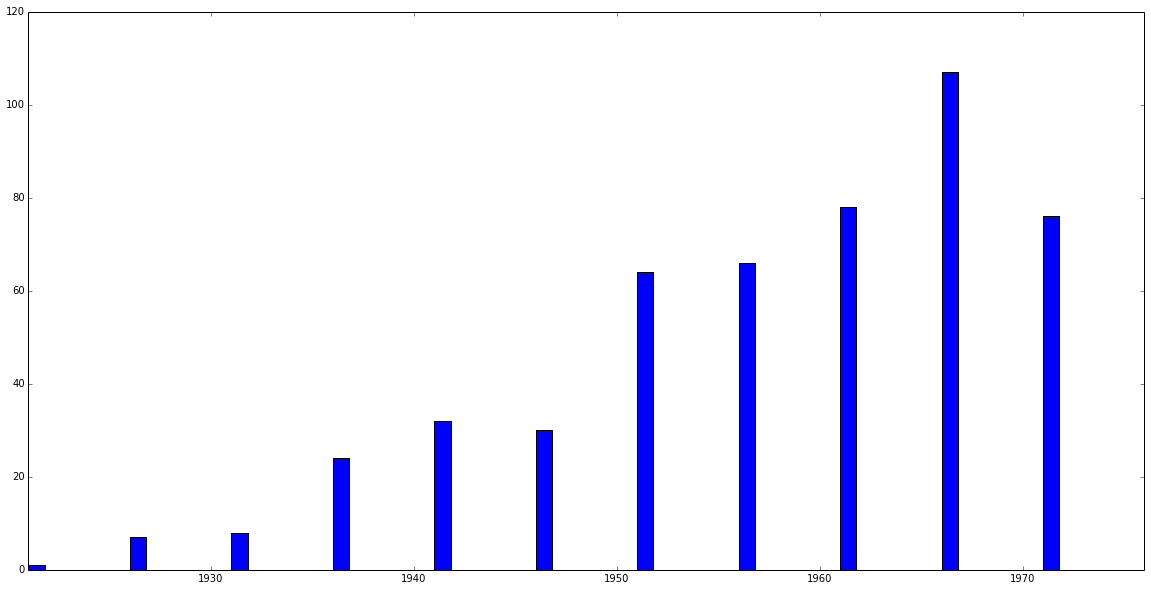
\includegraphics{corpus_plot_distribution.png}
\end{figure}

...or by both time and journal:

\begin{Verbatim}[commandchars=\\\{\}]
\PYG{g+gp}{\PYGZgt{}\PYGZgt{}\PYGZgt{} }\PYG{n}{C}\PYG{o}{.}\PYG{n}{plot\PYGZus{}distribution}\PYG{p}{(}\PYG{l+s}{\PYGZsq{}}\PYG{l+s}{date}\PYG{l+s}{\PYGZsq{}}\PYG{p}{,} \PYG{l+s}{\PYGZsq{}}\PYG{l+s}{jtitle}\PYG{l+s}{\PYGZsq{}}\PYG{p}{)}
\end{Verbatim}
\begin{figure}[htbp]
\centering

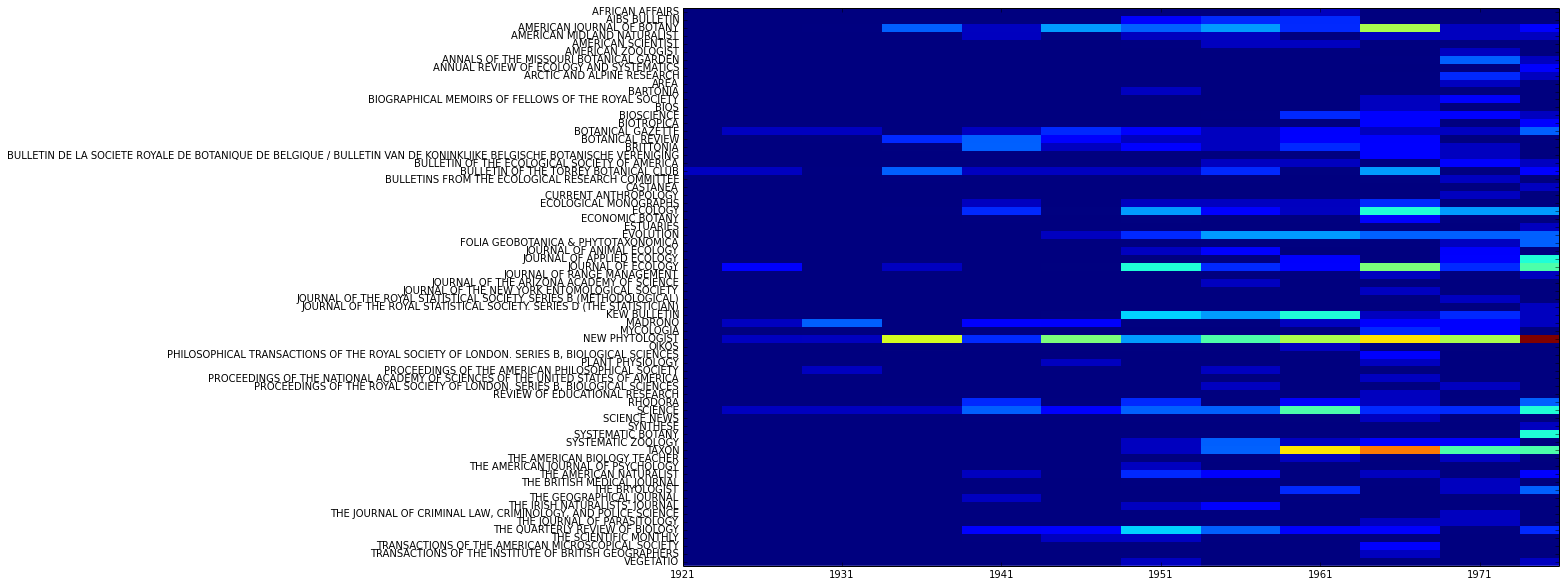
\includegraphics{corpus_plot_distribution_2d.png}
\end{figure}


\subsection{Simple networks simply}
\label{quickstart:simple-networks-simply}
Network-building methods are in {\hyperref[tethne.networks:module-tethne.networks]{\code{networks}}}. You can create a coauthorship
network like this:

\begin{Verbatim}[commandchars=\\\{\}]
\PYG{g+gp}{\PYGZgt{}\PYGZgt{}\PYGZgt{} }\PYG{k+kn}{from} \PYG{n+nn}{tethne.networks} \PYG{k+kn}{import} \PYG{n}{authors}
\PYG{g+gp}{\PYGZgt{}\PYGZgt{}\PYGZgt{} }\PYG{n}{coauthors} \PYG{o}{=} \PYG{n}{authors}\PYG{o}{.}\PYG{n}{coauthors}\PYG{p}{(}\PYG{n}{C}\PYG{p}{)}
\end{Verbatim}

To introduce a temporal component, slice your {\hyperref[tethne.classes.corpus:tethne.classes.corpus.Corpus]{\code{Corpus}}} and then create a {\hyperref[tethne.classes.graphcollection:tethne.classes.graphcollection.GraphCollection]{\code{GraphCollection}}} (\code{cumulative=True} means that the coauthorship network
will grow over time without losing old connections):

\begin{Verbatim}[commandchars=\\\{\}]
\PYG{g+gp}{\PYGZgt{}\PYGZgt{}\PYGZgt{} }\PYG{n}{C}\PYG{o}{.}\PYG{n}{slice}\PYG{p}{(}\PYG{l+s}{\PYGZsq{}}\PYG{l+s}{date}\PYG{l+s}{\PYGZsq{}}\PYG{p}{,} \PYG{l+s}{\PYGZsq{}}\PYG{l+s}{time\PYGZus{}period}\PYG{l+s}{\PYGZsq{}}\PYG{p}{,} \PYG{n}{window\PYGZus{}size}\PYG{o}{=}\PYG{l+m+mi}{5}\PYG{p}{,} \PYG{n}{cumulative}\PYG{o}{=}\PYG{n+nb+bp}{True}\PYG{p}{)}   \PYG{c}{\PYGZsh{} 5\PYGZhy{}year bins.}
\PYG{g+gp}{\PYGZgt{}\PYGZgt{}\PYGZgt{} }\PYG{k+kn}{from} \PYG{n+nn}{tethne} \PYG{k+kn}{import} \PYG{n}{GraphCollection}
\PYG{g+gp}{\PYGZgt{}\PYGZgt{}\PYGZgt{} }\PYG{n}{G} \PYG{o}{=} \PYG{n}{GraphCollection}\PYG{p}{(}\PYG{p}{)}\PYG{o}{.}\PYG{n}{build}\PYG{p}{(}\PYG{n}{C}\PYG{p}{,} \PYG{l+s}{\PYGZsq{}}\PYG{l+s}{date}\PYG{l+s}{\PYGZsq{}}\PYG{p}{,} \PYG{l+s}{\PYGZsq{}}\PYG{l+s}{authors}\PYG{l+s}{\PYGZsq{}}\PYG{p}{,} \PYG{l+s}{\PYGZsq{}}\PYG{l+s}{coauthors}\PYG{l+s}{\PYGZsq{}}\PYG{p}{)}
\end{Verbatim}

If you're using WoS data (with citations), you can also build citation-based graphs (see
{\hyperref[tethne.networks.papers:module-tethne.networks.papers]{\code{networks.papers}}}). Here's a static co-citation graph from a {\hyperref[tethne.classes.corpus:tethne.classes.corpus.Corpus]{\code{Corpus}}}:

\begin{Verbatim}[commandchars=\\\{\}]
\PYG{g+gp}{\PYGZgt{}\PYGZgt{}\PYGZgt{} }\PYG{n}{C}\PYG{o}{.}\PYG{n}{slice}\PYG{p}{(}\PYG{l+s}{\PYGZsq{}}\PYG{l+s}{date}\PYG{l+s}{\PYGZsq{}}\PYG{p}{,} \PYG{l+s}{\PYGZsq{}}\PYG{l+s}{time\PYGZus{}period}\PYG{l+s}{\PYGZsq{}}\PYG{p}{,} \PYG{n}{window\PYGZus{}size}\PYG{o}{=}\PYG{l+m+mi}{5}\PYG{p}{)}    \PYG{c}{\PYGZsh{} No need for {}`cumulative{}` here.}
\PYG{g+go}{\PYGZgt{}\PYGZgt{} from tethne.networks import papers}
\PYG{g+gp}{\PYGZgt{}\PYGZgt{}\PYGZgt{} }\PYG{n}{cocitation} \PYG{o}{=} \PYG{n}{papers}\PYG{o}{.}\PYG{n}{cocitation}\PYG{p}{(}\PYG{n}{C}\PYG{o}{.}\PYG{n}{all\PYGZus{}papers}\PYG{p}{(}\PYG{p}{)}\PYG{p}{,} \PYG{n}{threshold}\PYG{o}{=}\PYG{l+m+mi}{2}\PYG{p}{,} \PYG{n}{topn}\PYG{o}{=}\PYG{l+m+mi}{300}\PYG{p}{)}
\end{Verbatim}

\code{threshold=2} means that papers must be co-cited twice, and \code{topn=300} means that
only the top 300 most cited papers will be included.

To see a time-variant co-citation network, build a {\hyperref[tethne.classes.graphcollection:tethne.classes.graphcollection.GraphCollection]{\code{GraphCollection}}} just as
before:

\begin{Verbatim}[commandchars=\\\{\}]
\PYG{g+gp}{\PYGZgt{}\PYGZgt{}\PYGZgt{} }\PYG{n}{G} \PYG{o}{=} \PYG{n}{GraphCollection}\PYG{p}{(}\PYG{p}{)}\PYG{o}{.}\PYG{n}{build}\PYG{p}{(}\PYG{n}{C}\PYG{p}{,} \PYG{l+s}{\PYGZsq{}}\PYG{l+s}{date}\PYG{l+s}{\PYGZsq{}}\PYG{p}{,} \PYG{l+s}{\PYGZsq{}}\PYG{l+s}{papers}\PYG{l+s}{\PYGZsq{}}\PYG{p}{,} \PYG{l+s}{\PYGZsq{}}\PYG{l+s}{cocitation}\PYG{l+s}{\PYGZsq{}}\PYG{p}{,} \PYG{n}{threshold}\PYG{o}{=}\PYG{l+m+mi}{2}\PYG{p}{,} \PYG{n}{topn}\PYG{o}{=}\PYG{l+m+mi}{300}\PYG{p}{)}
\end{Verbatim}


\subsection{Visualize your networks}
\label{quickstart:visualize-your-networks}
You can export a graph for visualization in \href{http://cytoscape.org}{Cytoscape} using
{\hyperref[tethne.writers:module-tethne.writers]{\code{writers}}}:

\begin{Verbatim}[commandchars=\\\{\}]
\PYG{g+gp}{\PYGZgt{}\PYGZgt{}\PYGZgt{} }\PYG{k+kn}{from} \PYG{n+nn}{tethne.writers} \PYG{k+kn}{import} \PYG{n}{graph}
\PYG{g+gp}{\PYGZgt{}\PYGZgt{}\PYGZgt{} }\PYG{n}{graph}\PYG{o}{.}\PYG{n}{to\PYGZus{}graphml}\PYG{p}{(}\PYG{n}{coauthors}\PYG{p}{,} \PYG{l+s}{\PYGZsq{}}\PYG{l+s}{/path/to/my/graph.graphml}\PYG{l+s}{\PYGZsq{}}\PYG{p}{)}
\end{Verbatim}

To visualize a {\hyperref[tethne.classes.graphcollection:tethne.classes.graphcollection.GraphCollection]{\code{GraphCollection}}} as a dynamic graph in Cytoscape, export it using
{\hyperref[tethne.writers.collection:tethne.writers.collection.to_dxgmml]{\code{writers.collection.to\_dxgmml()}}}:

\begin{Verbatim}[commandchars=\\\{\}]
\PYG{g+gp}{\PYGZgt{}\PYGZgt{}\PYGZgt{} }\PYG{k+kn}{from} \PYG{n+nn}{tethne.writers} \PYG{k+kn}{import} \PYG{n}{collection}
\PYG{g+gp}{\PYGZgt{}\PYGZgt{}\PYGZgt{} }\PYG{n}{collection}\PYG{o}{.}\PYG{n}{to\PYGZus{}dxgmml}\PYG{p}{(}\PYG{n}{G}\PYG{p}{,} \PYG{l+s}{\PYGZsq{}}\PYG{l+s}{/path/to/my/dynamicNetwork.xgmml}\PYG{l+s}{\PYGZsq{}}\PYG{p}{)}
\end{Verbatim}


\subsection{Working with Words}
\label{quickstart:working-with-words}
Suppose you loaded up a {\hyperref[tethne.classes.corpus:tethne.classes.corpus.Corpus]{\code{Corpus}}} from some DfR datasets, using:

\begin{Verbatim}[commandchars=\\\{\}]
\PYG{g+gp}{\PYGZgt{}\PYGZgt{}\PYGZgt{} }\PYG{k+kn}{from} \PYG{n+nn}{tethne.readers} \PYG{k+kn}{import} \PYG{n}{dfr}
\PYG{g+gp}{\PYGZgt{}\PYGZgt{}\PYGZgt{} }\PYG{n}{C} \PYG{o}{=} \PYG{n}{dfr}\PYG{o}{.}\PYG{n}{corpus\PYGZus{}from\PYGZus{}dir}\PYG{p}{(}\PYG{l+s}{\PYGZsq{}}\PYG{l+s}{/path/to/my/dataset}\PYG{l+s}{\PYGZsq{}}\PYG{p}{,} \PYG{l+s}{\PYGZsq{}}\PYG{l+s}{uni}\PYG{l+s}{\PYGZsq{}}\PYG{p}{)}
\end{Verbatim}

Now you have some \code{'unigrams'} in \code{C.features}. There are surely plenty of junk words
in there. You can apply a stoplist when you load the {\hyperref[tethne.classes.corpus:tethne.classes.corpus.Corpus]{\code{Corpus}}}, by passing it to
\code{exclude}:

\begin{Verbatim}[commandchars=\\\{\}]
\PYG{g+gp}{\PYGZgt{}\PYGZgt{}\PYGZgt{} }\PYG{k+kn}{from} \PYG{n+nn}{nltk.corpus} \PYG{k+kn}{import} \PYG{n}{stopwords}
\PYG{g+gp}{\PYGZgt{}\PYGZgt{}\PYGZgt{} }\PYG{n}{stoplist} \PYG{o}{=} \PYG{n}{stopwords}\PYG{o}{.}\PYG{n}{words}\PYG{p}{(}\PYG{p}{)}
\PYG{g+gp}{\PYGZgt{}\PYGZgt{}\PYGZgt{} }\PYG{k+kn}{from} \PYG{n+nn}{tethne.readers} \PYG{k+kn}{import} \PYG{n}{dfr}
\PYG{g+gp}{\PYGZgt{}\PYGZgt{}\PYGZgt{} }\PYG{n}{C} \PYG{o}{=} \PYG{n}{dfr}\PYG{o}{.}\PYG{n}{corpus\PYGZus{}from\PYGZus{}dir}\PYG{p}{(}\PYG{l+s}{\PYGZsq{}}\PYG{l+s}{/path/to/my/dataset}\PYG{l+s}{\PYGZsq{}}\PYG{p}{,} \PYG{l+s}{\PYGZsq{}}\PYG{l+s}{uni}\PYG{l+s}{\PYGZsq{}}\PYG{p}{,} \PYG{n}{exclude}\PYG{o}{=}\PYG{n}{stoplist}\PYG{p}{)}
\end{Verbatim}

If you have some recent WoS data with abstracts, you can get a featureset from abstract
terms, too:

\begin{Verbatim}[commandchars=\\\{\}]
\PYG{g+gp}{\PYGZgt{}\PYGZgt{}\PYGZgt{} }\PYG{k+kn}{from} \PYG{n+nn}{tethne.readers} \PYG{k+kn}{import} \PYG{n}{wos}
\PYG{g+gp}{\PYGZgt{}\PYGZgt{}\PYGZgt{} }\PYG{n}{C} \PYG{o}{=} \PYG{n}{dfr}\PYG{o}{.}\PYG{n}{read\PYGZus{}corpus}\PYG{p}{(}\PYG{l+s}{\PYGZsq{}}\PYG{l+s}{/path/to/my/wosdata.txt}\PYG{l+s}{\PYGZsq{}}\PYG{p}{)}
\PYG{g+gp}{\PYGZgt{}\PYGZgt{}\PYGZgt{} }\PYG{n}{C}\PYG{o}{.}\PYG{n}{abstract\PYGZus{}to\PYGZus{}features}\PYG{p}{(}\PYG{p}{)} \PYG{c}{\PYGZsh{} Automatically applies a stoplist.}
\end{Verbatim}

Filter the words in the {\hyperref[tethne.classes.corpus:tethne.classes.corpus.Corpus]{\code{Corpus}}} further, using \code{Corpus.filter\_features()}.
Maybe you only want words that occur more than three times overall, occur in more than one
document, and are at least four characters in length.

\begin{Verbatim}[commandchars=\\\{\}]
\PYG{g+gp}{\PYGZgt{}\PYGZgt{}\PYGZgt{} }\PYG{k}{def} \PYG{n+nf}{filt}\PYG{p}{(}\PYG{n}{s}\PYG{p}{,} \PYG{n}{C}\PYG{p}{,} \PYG{n}{DC}\PYG{p}{)}\PYG{p}{:}
\PYG{g+gp}{... }    \PYG{k}{if} \PYG{n}{C} \PYG{o}{\PYGZgt{}} \PYG{l+m+mi}{3} \PYG{o+ow}{and} \PYG{n}{DC} \PYG{o}{\PYGZgt{}} \PYG{l+m+mi}{1} \PYG{o+ow}{and} \PYG{n+nb}{len}\PYG{p}{(}\PYG{n}{s}\PYG{p}{)} \PYG{o}{\PYGZgt{}} \PYG{l+m+mi}{3}\PYG{p}{:}
\PYG{g+gp}{... }        \PYG{k}{return} \PYG{n+nb+bp}{True}
\PYG{g+gp}{... }    \PYG{k}{return} \PYG{n+nb+bp}{False}
\PYG{g+gp}{\PYGZgt{}\PYGZgt{}\PYGZgt{} }\PYG{n}{C}\PYG{o}{.}\PYG{n}{filter\PYGZus{}features}\PYG{p}{(}\PYG{l+s}{\PYGZsq{}}\PYG{l+s}{unigrams}\PYG{l+s}{\PYGZsq{}}\PYG{p}{,} \PYG{l+s}{\PYGZsq{}}\PYG{l+s}{wordcounts\PYGZus{}filtered}\PYG{l+s}{\PYGZsq{}}\PYG{p}{,} \PYG{n}{filt}\PYG{p}{)}
\end{Verbatim}

You can see how the word \code{four} is distributed across your {\hyperref[tethne.classes.corpus:tethne.classes.corpus.Corpus]{\code{Corpus}}} using
\code{Corpus.plot\_distribution()}:

\begin{Verbatim}[commandchars=\\\{\}]
\PYG{g+gp}{\PYGZgt{}\PYGZgt{}\PYGZgt{} }\PYG{n}{C}\PYG{o}{.}\PYG{n}{slice}\PYG{p}{(}\PYG{l+s}{\PYGZsq{}}\PYG{l+s}{date}\PYG{l+s}{\PYGZsq{}}\PYG{p}{,} \PYG{n}{method}\PYG{o}{=}\PYG{l+s}{\PYGZsq{}}\PYG{l+s}{time\PYGZus{}period}\PYG{l+s}{\PYGZsq{}}\PYG{p}{,} \PYG{n}{window\PYGZus{}size}\PYG{o}{=}\PYG{l+m+mi}{5}\PYG{p}{)}
\PYG{g+gp}{\PYGZgt{}\PYGZgt{}\PYGZgt{} }\PYG{n}{C}\PYG{o}{.}\PYG{n}{slice}\PYG{p}{(}\PYG{l+s}{\PYGZsq{}}\PYG{l+s}{jtitle}\PYG{l+s}{\PYGZsq{}}\PYG{p}{)}
\PYG{g+gp}{\PYGZgt{}\PYGZgt{}\PYGZgt{} }\PYG{n}{fkwargs} \PYG{o}{=} \PYG{p}{\PYGZob{}}
\PYG{g+gp}{... }    \PYG{l+s}{\PYGZsq{}}\PYG{l+s}{featureset}\PYG{l+s}{\PYGZsq{}}\PYG{p}{:} \PYG{l+s}{\PYGZsq{}}\PYG{l+s}{wordcounts\PYGZus{}filtered}\PYG{l+s}{\PYGZsq{}}\PYG{p}{,}
\PYG{g+gp}{... }    \PYG{l+s}{\PYGZsq{}}\PYG{l+s}{feature}\PYG{l+s}{\PYGZsq{}}\PYG{p}{:} \PYG{l+s}{\PYGZsq{}}\PYG{l+s}{four}\PYG{l+s}{\PYGZsq{}}\PYG{p}{,}
\PYG{g+gp}{... }    \PYG{l+s}{\PYGZsq{}}\PYG{l+s}{mode}\PYG{l+s}{\PYGZsq{}}\PYG{p}{:} \PYG{l+s}{\PYGZsq{}}\PYG{l+s}{counts}\PYG{l+s}{\PYGZsq{}}\PYG{p}{,}
\PYG{g+gp}{... }    \PYG{l+s}{\PYGZsq{}}\PYG{l+s}{normed}\PYG{l+s}{\PYGZsq{}}\PYG{p}{:} \PYG{n+nb+bp}{True}\PYG{p}{,}
\PYG{g+gp}{... }    \PYG{p}{\PYGZcb{}}
\PYG{g+gp}{\PYGZgt{}\PYGZgt{}\PYGZgt{} }\PYG{n}{fig} \PYG{o}{=} \PYG{n}{C}\PYG{o}{.}\PYG{n}{plot\PYGZus{}distribution}\PYG{p}{(}\PYG{l+s}{\PYGZsq{}}\PYG{l+s}{date}\PYG{l+s}{\PYGZsq{}}\PYG{p}{,} \PYG{l+s}{\PYGZsq{}}\PYG{l+s}{jtitle}\PYG{l+s}{\PYGZsq{}}\PYG{p}{,} \PYG{n}{mode}\PYG{o}{=}\PYG{l+s}{\PYGZsq{}}\PYG{l+s}{features}\PYG{l+s}{\PYGZsq{}}\PYG{p}{,}
\PYG{g+go}{                              fkwargs=fkwargs, interpolation=\PYGZsq{}none\PYGZsq{})}
\PYG{g+gp}{\PYGZgt{}\PYGZgt{}\PYGZgt{} }\PYG{n}{fig}\PYG{o}{.}\PYG{n}{savefig}\PYG{p}{(}\PYG{l+s}{\PYGZsq{}}\PYG{l+s}{/path/to/dist.png}\PYG{l+s}{\PYGZsq{}}\PYG{p}{)}
\end{Verbatim}
\begin{figure}[htbp]
\centering

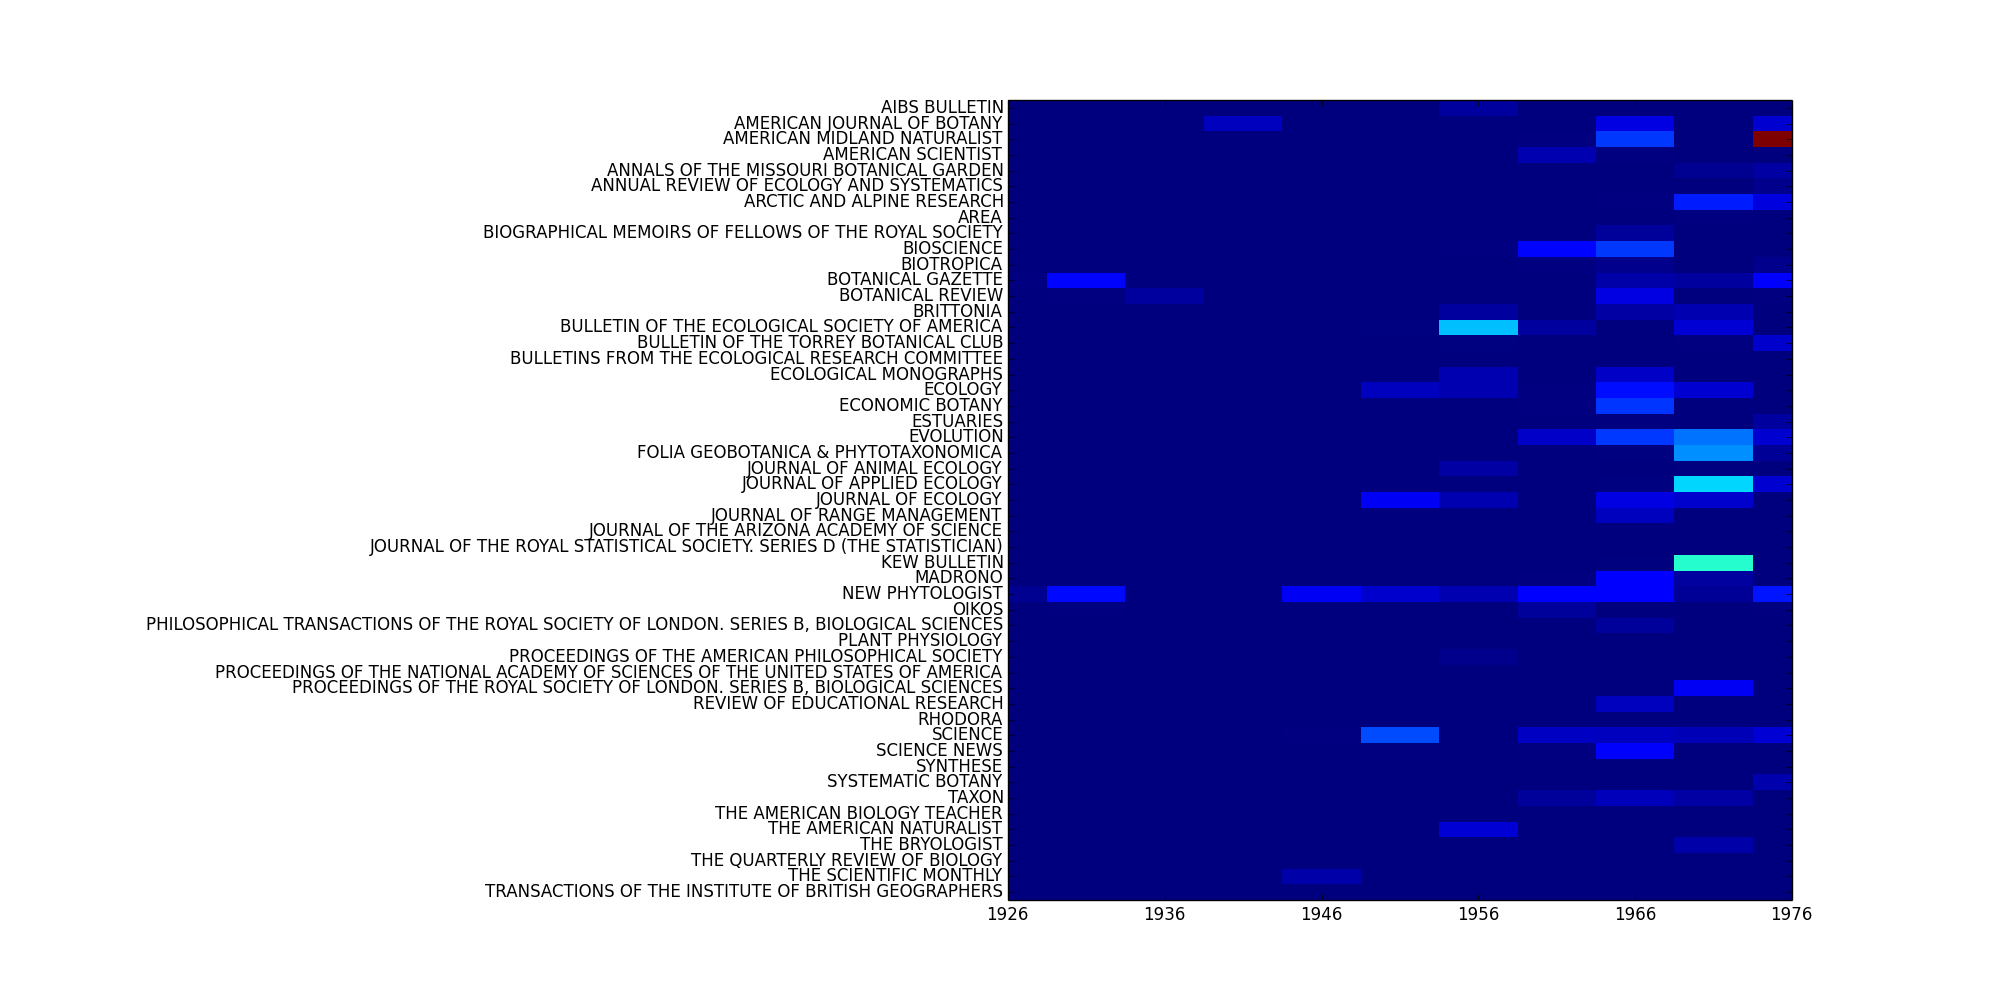
\includegraphics{testdist.png}
\end{figure}


\subsection{Models Based on Words}
\label{quickstart:models-based-on-words}
Topic models are pretty popular. You can create a LDA topic model with MALLET
using a {\hyperref[tethne.model.managers.mallet:tethne.model.managers.mallet.MALLETModelManager]{\code{MALLETModelManager}}}. First, get the manager:

\begin{Verbatim}[commandchars=\\\{\}]
\PYG{g+gp}{\PYGZgt{}\PYGZgt{}\PYGZgt{} }\PYG{k+kn}{from} \PYG{n+nn}{tethne.model} \PYG{k+kn}{import} \PYG{n}{MALLETModelManager}
\PYG{g+gp}{\PYGZgt{}\PYGZgt{}\PYGZgt{} }\PYG{n}{outpath} \PYG{o}{=} \PYG{l+s}{\PYGZsq{}}\PYG{l+s}{/path/to/my/working/directory}\PYG{l+s}{\PYGZsq{}}
\PYG{g+gp}{\PYGZgt{}\PYGZgt{}\PYGZgt{} }\PYG{n}{mallet} \PYG{o}{=} \PYG{l+s}{\PYGZsq{}}\PYG{l+s}{/Applications/mallet\PYGZhy{}2.0.7}\PYG{l+s}{\PYGZsq{}}    \PYG{c}{\PYGZsh{} Path to MALLET install directory.}
\PYG{g+gp}{\PYGZgt{}\PYGZgt{}\PYGZgt{} }\PYG{n}{M} \PYG{o}{=} \PYG{n}{MALLETModelManager}\PYG{p}{(}\PYG{n}{C}\PYG{p}{,} \PYG{l+s}{\PYGZsq{}}\PYG{l+s}{wordcounts\PYGZus{}filtered}\PYG{l+s}{\PYGZsq{}}\PYG{p}{,} \PYG{n}{outpath}\PYG{p}{,} \PYG{n}{mallet\PYGZus{}path}\PYG{o}{=}\PYG{n}{mallet}\PYG{p}{)}
\end{Verbatim}

Now \code{prep} and \code{build}. Here's an example for 50 topics:

\begin{Verbatim}[commandchars=\\\{\}]
\PYG{g+gp}{\PYGZgt{}\PYGZgt{}\PYGZgt{} }\PYG{n}{M}\PYG{o}{.}\PYG{n}{prep}\PYG{p}{(}\PYG{p}{)}
\PYG{g+gp}{\PYGZgt{}\PYGZgt{}\PYGZgt{} }\PYG{n}{model} \PYG{o}{=} \PYG{n}{M}\PYG{o}{.}\PYG{n}{build}\PYG{p}{(}\PYG{n}{Z}\PYG{o}{=}\PYG{l+m+mi}{50}\PYG{p}{,} \PYG{n}{max\PYGZus{}iter}\PYG{o}{=}\PYG{l+m+mi}{300}\PYG{p}{)}  \PYG{c}{\PYGZsh{} May take a while.}
\end{Verbatim}

Here are the top 5 words in topic 1:

\begin{Verbatim}[commandchars=\\\{\}]
\PYG{g+gp}{\PYGZgt{}\PYGZgt{}\PYGZgt{} }\PYG{n}{model}\PYG{o}{.}\PYG{n}{print\PYGZus{}topic}\PYG{p}{(}\PYG{l+m+mi}{1}\PYG{p}{,} \PYG{n}{Nwords}\PYG{o}{=}\PYG{l+m+mi}{5}\PYG{p}{)}
\PYG{g+go}{\PYGZsq{}opposed, terminates, trichinosis, cistus, acaule\PYGZsq{}}
\end{Verbatim}

To view the representation of topic 1 over the slices in the {\hyperref[tethne.classes.corpus:tethne.classes.corpus.Corpus]{\code{Corpus}}}...

\begin{Verbatim}[commandchars=\\\{\}]
\PYG{g+gp}{\PYGZgt{}\PYGZgt{}\PYGZgt{} }\PYG{n}{keys}\PYG{p}{,} \PYG{n+nb}{repr} \PYG{o}{=} \PYG{n}{M}\PYG{o}{.}\PYG{n}{topic\PYGZus{}over\PYGZus{}time}\PYG{p}{(}\PYG{l+m+mi}{1}\PYG{p}{,} \PYG{n}{plot}\PYG{o}{=}\PYG{n+nb+bp}{True}\PYG{p}{)}
\end{Verbatim}

...which should return \code{keys} (date) and \code{repr} (\% documents) for topic 1,
and generate a plot like this one in your \code{outpath}.
\begin{figure}[htbp]
\centering

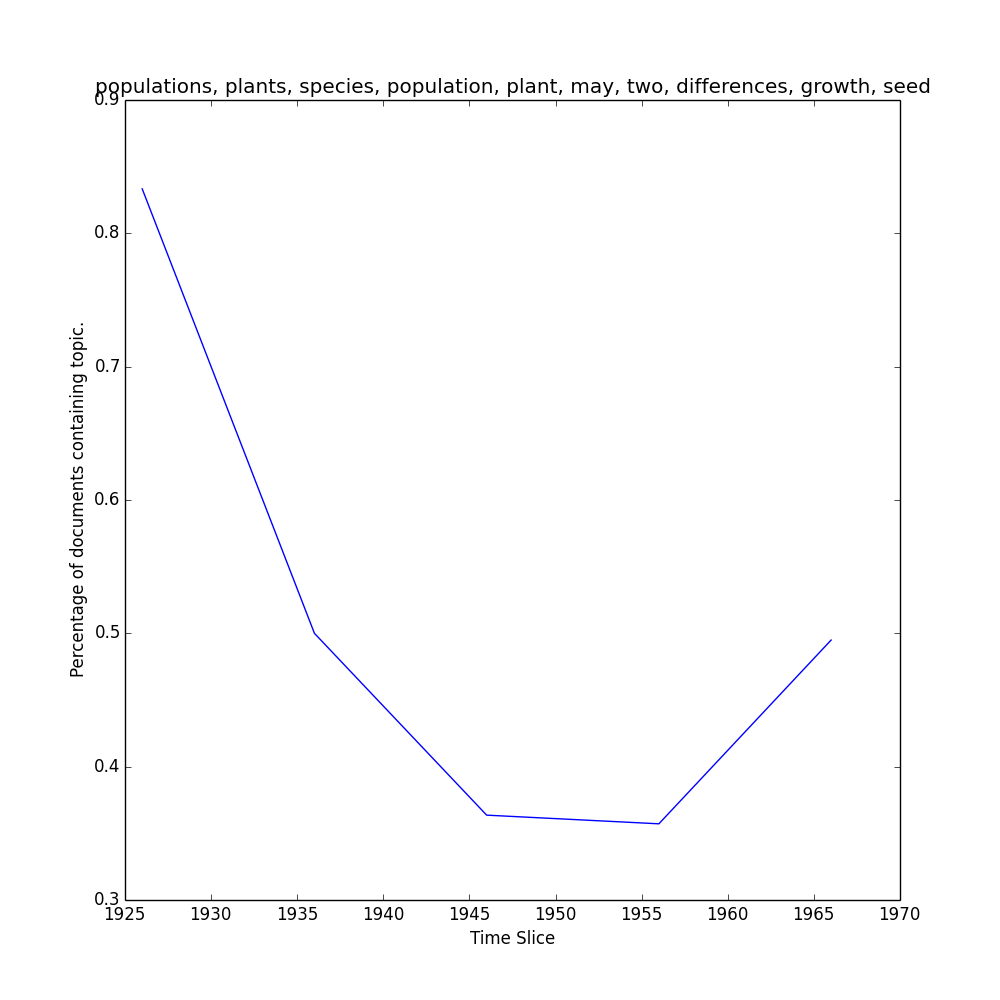
\includegraphics{topic_1_over_time.png}
\end{figure}


\subsection{Combining corpus models and social models}
\label{quickstart:combining-corpus-models-and-social-models}
Social models (see {\hyperref[tethne.model.social:module-tethne.model.social]{\code{model.social}}}) represent the dynamics of social influence
in terms of behavior adoption. Writing about a topic is a behavior.

Suppose you have a coauthorship {\hyperref[tethne.classes.graphcollection:tethne.classes.graphcollection.GraphCollection]{\code{GraphCollection}}}...

\begin{Verbatim}[commandchars=\\\{\}]
\PYG{g+gp}{\PYGZgt{}\PYGZgt{}\PYGZgt{} }\PYG{n}{C}\PYG{o}{.}\PYG{n}{slice}\PYG{p}{(}\PYG{l+s}{\PYGZsq{}}\PYG{l+s}{date}\PYG{l+s}{\PYGZsq{}}\PYG{p}{,} \PYG{l+s}{\PYGZsq{}}\PYG{l+s}{time\PYGZus{}period}\PYG{l+s}{\PYGZsq{}}\PYG{p}{,} \PYG{n}{window\PYGZus{}size}\PYG{o}{=}\PYG{l+m+mi}{5}\PYG{p}{,} \PYG{n}{cumulative}\PYG{o}{=}\PYG{n+nb+bp}{True}\PYG{p}{)}
\PYG{g+gp}{\PYGZgt{}\PYGZgt{}\PYGZgt{} }\PYG{k+kn}{from} \PYG{n+nn}{tethne} \PYG{k+kn}{import} \PYG{n}{GraphCollection}
\PYG{g+gp}{\PYGZgt{}\PYGZgt{}\PYGZgt{} }\PYG{n}{G} \PYG{o}{=} \PYG{n}{GraphCollection}\PYG{p}{(}\PYG{p}{)}\PYG{o}{.}\PYG{n}{build}\PYG{p}{(}\PYG{n}{C}\PYG{p}{,} \PYG{l+s}{\PYGZsq{}}\PYG{l+s}{date}\PYG{l+s}{\PYGZsq{}}\PYG{p}{,} \PYG{l+s}{\PYGZsq{}}\PYG{l+s}{authors}\PYG{l+s}{\PYGZsq{}}\PYG{p}{,} \PYG{l+s}{\PYGZsq{}}\PYG{l+s}{coauthors}\PYG{l+s}{\PYGZsq{}}\PYG{p}{)}
\end{Verbatim}

...and the {\hyperref[tethne.model.corpus.ldamodel:tethne.model.corpus.ldamodel.LDAModel]{\code{LDAModel}}} (\code{model}) from the last section.

You can use the {\hyperref[tethne.model.managers.tap:tethne.model.managers.tap.TAPModelManager]{\code{TAPModelManager}}} to generate a {\hyperref[tethne.model.social.tapmodel:tethne.model.social.tapmodel.TAPModel]{\code{TAPModel}}}, which
represents a Topical Affinity Propagation social influence model.

\begin{Verbatim}[commandchars=\\\{\}]
\PYG{g+gp}{\PYGZgt{}\PYGZgt{}\PYGZgt{} }\PYG{k+kn}{from} \PYG{n+nn}{tethne.model} \PYG{k+kn}{import} \PYG{n}{TAPModelManager}
\PYG{g+gp}{\PYGZgt{}\PYGZgt{}\PYGZgt{} }\PYG{n}{T} \PYG{o}{=} \PYG{n}{TAPModelManager}\PYG{p}{(}\PYG{n}{C}\PYG{p}{,} \PYG{n}{G}\PYG{p}{,} \PYG{n}{model}\PYG{p}{)}
\PYG{g+gp}{\PYGZgt{}\PYGZgt{}\PYGZgt{} }\PYG{n}{T}\PYG{o}{.}\PYG{n}{build}\PYG{p}{(}\PYG{p}{)}                \PYG{c}{\PYGZsh{} This may take a while.}
\end{Verbatim}

You can get the social influence {\hyperref[tethne.classes.graphcollection:tethne.classes.graphcollection.GraphCollection]{\code{GraphCollection}}} for topic 1:

\begin{Verbatim}[commandchars=\\\{\}]
\PYG{g+gp}{\PYGZgt{}\PYGZgt{}\PYGZgt{} }\PYG{n}{IG} \PYG{o}{=} \PYG{n}{T}\PYG{o}{.}\PYG{n}{graph\PYGZus{}collection}\PYG{p}{(}\PYG{l+m+mi}{0}\PYG{p}{)}
\end{Verbatim}

Since you used \code{cumulative=True} when creating the coauthors {\hyperref[tethne.classes.graphcollection:tethne.classes.graphcollection.GraphCollection]{\code{GraphCollection}}},
the latest graph in the social influence GraphCollection is the most interesting:

\begin{Verbatim}[commandchars=\\\{\}]
\PYG{g+gp}{\PYGZgt{}\PYGZgt{}\PYGZgt{} }\PYG{n}{ig} \PYG{o}{=} \PYG{n}{IG}\PYG{p}{[}\PYG{n+nb}{sorted}\PYG{p}{(}\PYG{n}{IG}\PYG{o}{.}\PYG{n}{graphs}\PYG{o}{.}\PYG{n}{keys}\PYG{p}{(}\PYG{p}{)}\PYG{p}{)}\PYG{p}{[}\PYG{o}{\PYGZhy{}}\PYG{l+m+mi}{1}\PYG{p}{]}\PYG{p}{]}
\end{Verbatim}

Write it to GraphML:

\begin{Verbatim}[commandchars=\\\{\}]
\PYG{g+gp}{\PYGZgt{}\PYGZgt{}\PYGZgt{} }\PYG{k+kn}{from} \PYG{n+nn}{tethne.writers} \PYG{k+kn}{import} \PYG{n}{graph}
\PYG{g+gp}{\PYGZgt{}\PYGZgt{}\PYGZgt{} }\PYG{n}{graph}\PYG{o}{.}\PYG{n}{to\PYGZus{}graphml}\PYG{p}{(}\PYG{n}{ig}\PYG{p}{,} \PYG{l+s}{\PYGZsq{}}\PYG{l+s}{/path/to/my/graph.graphml}\PYG{l+s}{\PYGZsq{}}\PYG{p}{)}
\end{Verbatim}

And then visualize it in \href{http://www.cytoscape.org}{Cytoscape} or \href{http://gephi.org}{Gephi}.
\begin{figure}[htbp]
\centering

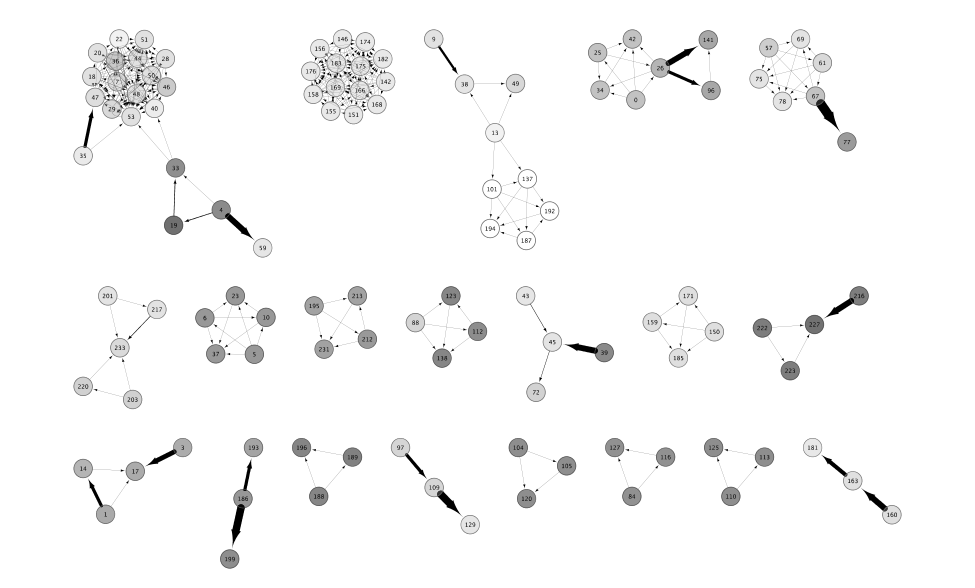
\includegraphics{tap_topic0.png}
\end{figure}


\section{Tutorials}
\label{tutorials:tutorials}\label{tutorials::doc}

\subsection{Getting Bibliographic Data}
\label{tutorial.getting_data:getting-bibliographic-data}\label{tutorial.getting_data:gettingdata}\label{tutorial.getting_data::doc}
The current version of Tethne supports bibliographic data from the ISI Web of Science,
Scopus, and JSTOR's Data-for-Research portal. Future releases will support data from
PubMed.
\setbox0\vbox{
\begin{minipage}{0.95\linewidth}
\begin{itemize}
\item {} 
{\hyperref[tutorial.getting_data:web-of-science]{Web of Science}}
\begin{itemize}
\item {} 
{\hyperref[tutorial.getting_data:structure-of-the-wos-field-tagged-data-file]{Structure of the WoS Field-Tagged Data File}}

\end{itemize}

\item {} 
{\hyperref[tutorial.getting_data:jstor-data-for-research]{JSTOR Data-for-Research}}

\item {} 
{\hyperref[tutorial.getting_data:scopus]{Scopus}}

\end{itemize}
\end{minipage}}
\begin{center}\setlength{\fboxsep}{5pt}\shadowbox{\box0}\end{center}


\subsubsection{Web of Science}
\label{tutorial.getting_data:web-of-science}
The ISI Web of Science is a proprietary database owned by Thompson Reuters.
If you are affiliated with an academic institution, you may have access to
this database via an institutional license.

For information about loading WoS data in Tethne, see the {\hyperref[tethne.readers.wos:module-tethne.readers.wos]{\code{readers.wos}}} module.

To access the Web of Science database via the Arizona State University library,
find the Web of Science \href{http://library.lib.asu.edu/record=e1000458}{entry} in the library's online catalog. You may be prompted
to log in to the University's Central Authentication System.

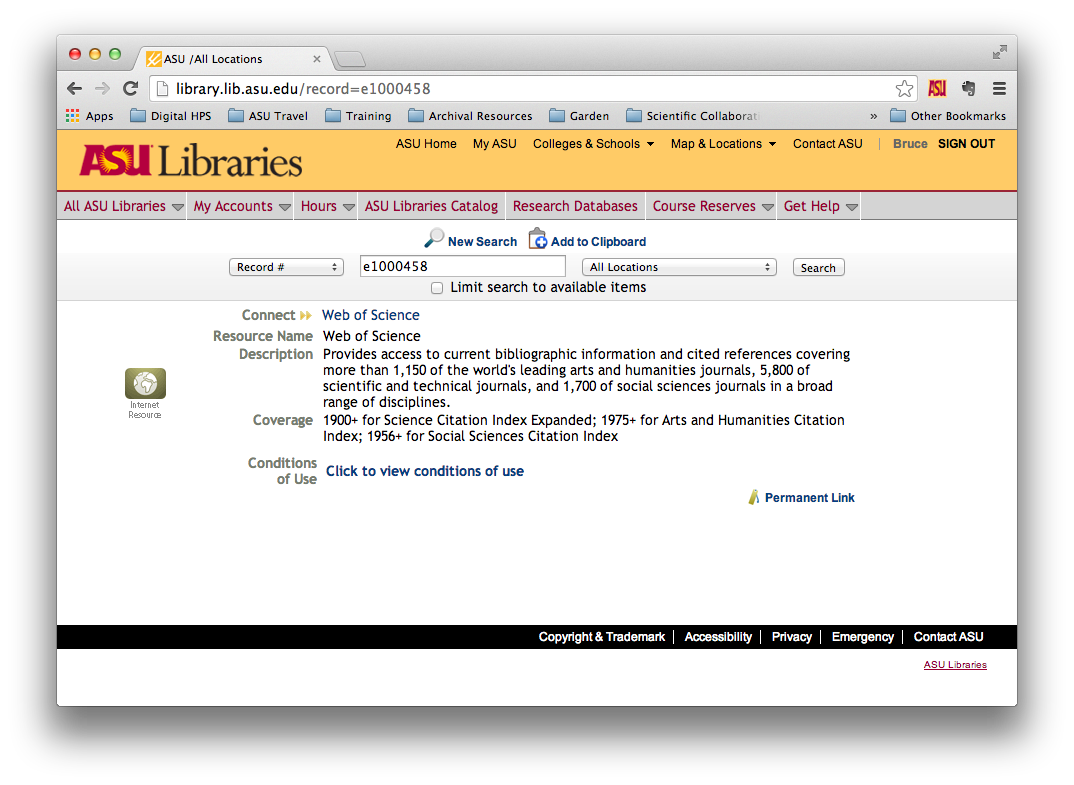
\includegraphics[width=0.600\linewidth]{getting.0.png}

Perform a search for literature of interest using the interface provided.

Your search criteria will be informed by the objectives of your research project. If you
are attempting to characterize the development of a research field, for example, you
should choose terms that pick out that field as uniquely as possible (consider using the
\code{Publication Name} search field). You can also pick out literatures originating from
particular institutions, by using the \code{Organization-Enhanced} search field.

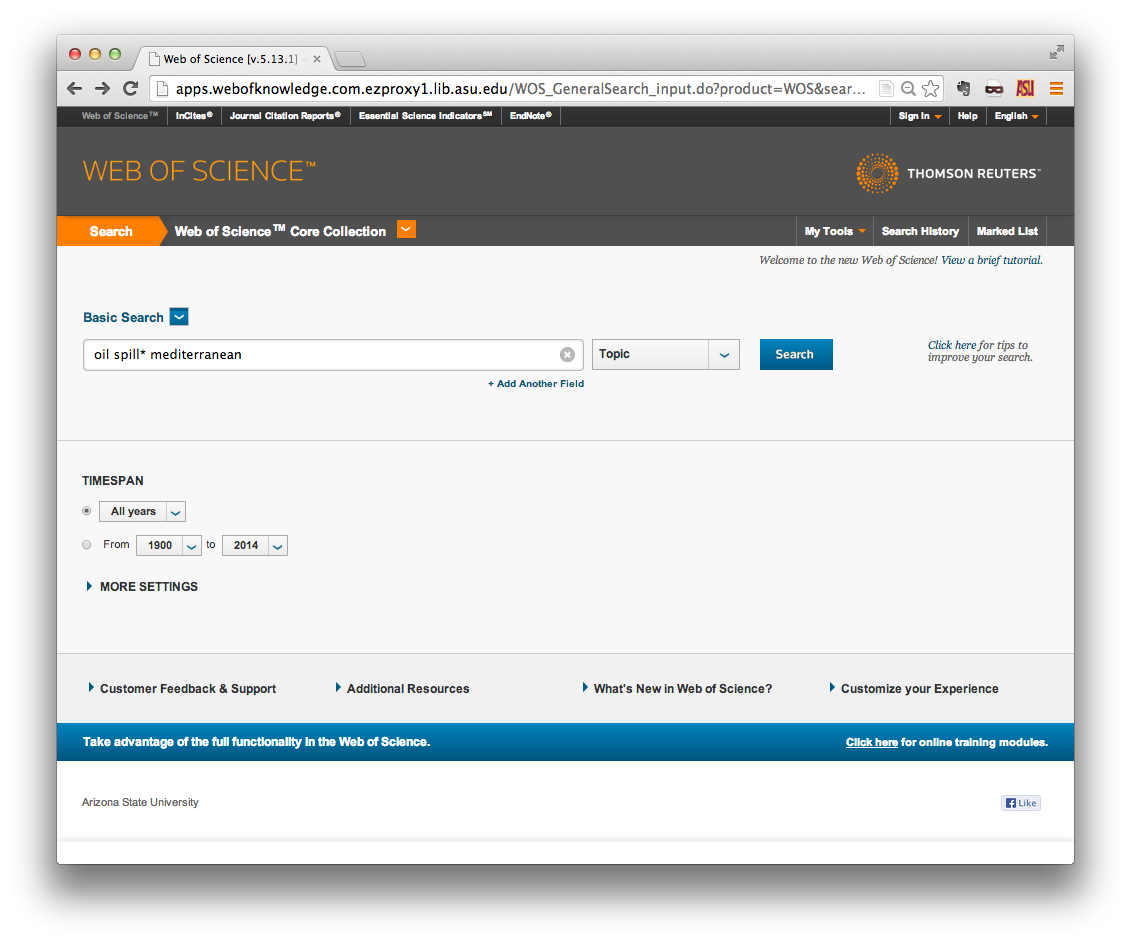
\includegraphics[width=0.600\linewidth]{getting.1.png}

Note also that you can restrict your research to one of three indexes in the Web of Science Core Collection:
\begin{itemize}
\item {} 
Science Citation Index Expanded is the largest index, containing scientific
publications from 1900 onward.

\item {} 
Social Sciences Citation Index covers 1956 onward.

\item {} 
Arts \& Humanities Citation Index is the smallest index, containing publications from
1975 onward.

\end{itemize}

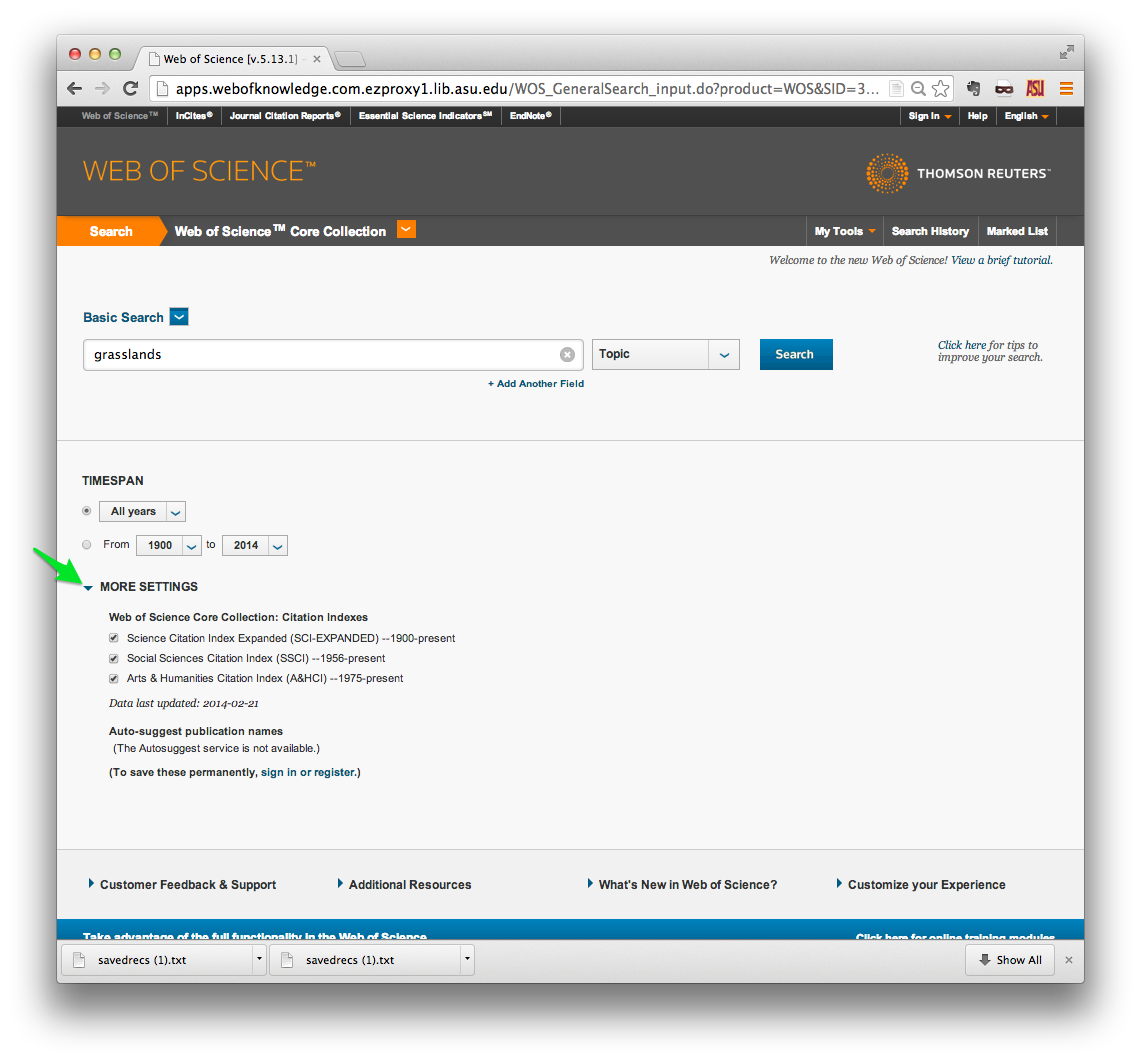
\includegraphics[width=0.600\linewidth]{getting.1.2.png}

Once you have found the papers that you are interested in, find the \code{Send to:} menu
at the top of the list of results. Click the small orange down-arrow, and select
\code{Other File Formats}.

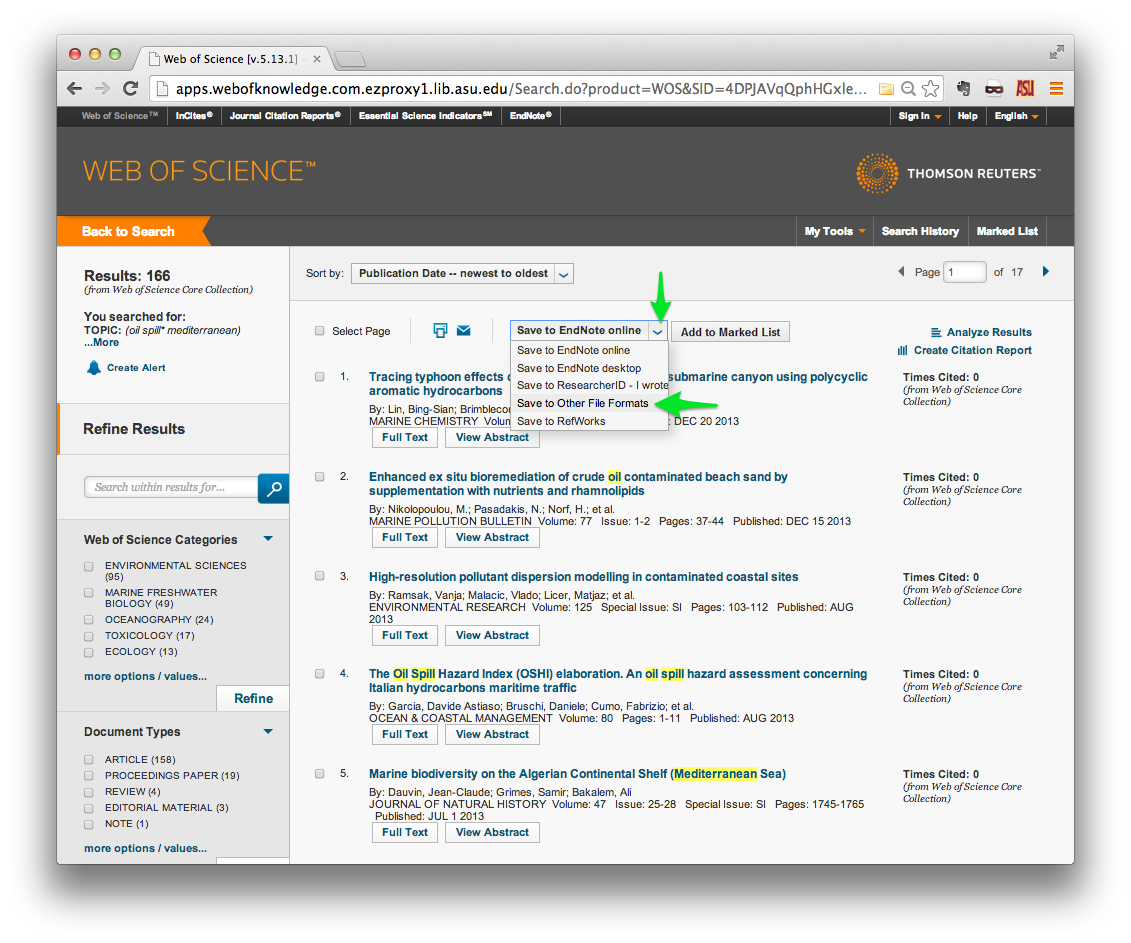
\includegraphics[width=0.600\linewidth]{getting.2.png}

A small in-browser window should open in the foreground. Specify the range of
records that you wish to download. \textbf{Note that you can only download 500 records
at a time}, so you may have to make multiple download requests. Be sure to specify
\code{Full Record and Cited References} in the \emph{Record Content} field, and \code{Plain Text}
in the \emph{File Format} field. Then click \code{Send}.

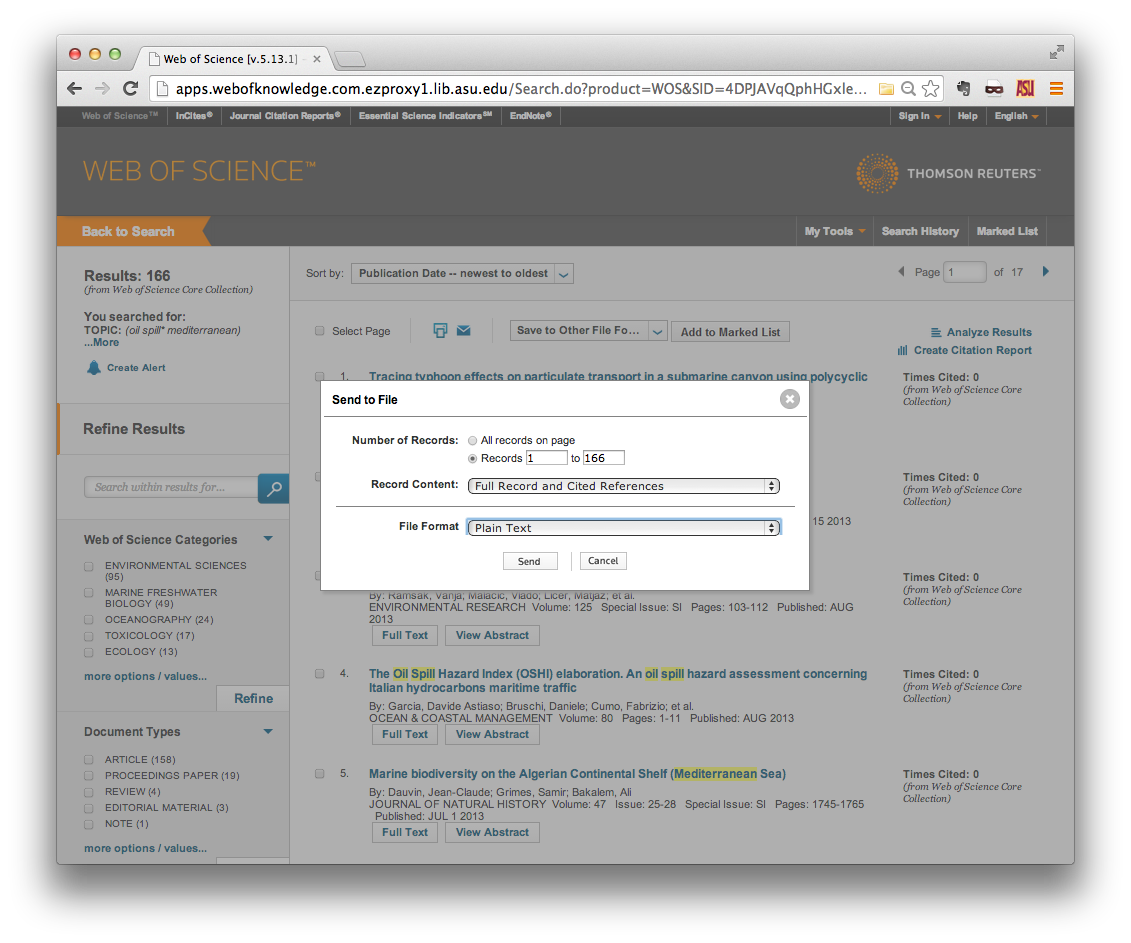
\includegraphics[width=0.600\linewidth]{getting.3.png}

After a few moments, a download should begin. WoS usually returns a field-tagged
data file called \code{savedrecs.txt}. Put this in a location on your filesystem where
you can find it later; this is the input for Tethne's WoS reader methods.

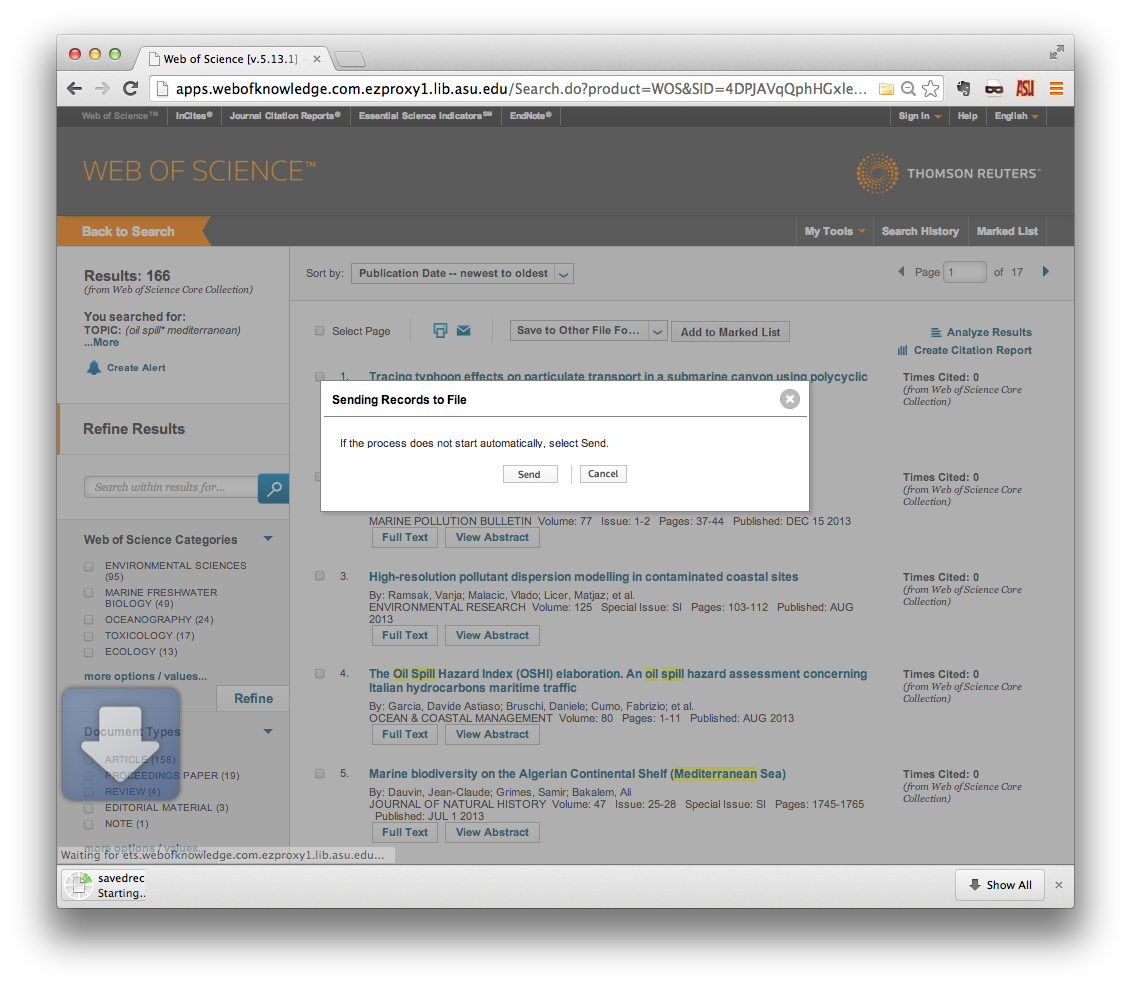
\includegraphics[width=0.600\linewidth]{getting.4.png}


\paragraph{Structure of the WoS Field-Tagged Data File}
\label{tutorial.getting_data:structure-of-the-wos-field-tagged-data-file}\label{tutorial.getting_data:fieldtagged}
If you open the text file returned by the WoS database (usually named `savedrecs.txt'),
you should see a whole bunch of field-tagged data. ``Field-tagged'' means that each metadata
field is denoted by a ``tag'' (a two-letter code), followed by values for that field. A
complete list of WoS field tags can be found \href{http://images.webofknowledge.com/WOKRS53B4/help/WOS/hs\_wos\_fieldtags.html}{here}. For best results, you should avoid
making changes to the contents of WoS data files.

The metadata record for each paper in your data file should begin with:

\begin{Verbatim}[commandchars=\\\{\}]
PT J
\end{Verbatim}

...and end with:

\begin{Verbatim}[commandchars=\\\{\}]
ER
\end{Verbatim}

There are two author fields: the AU field is always provided, and values take the form
``Last, FI''. AF is provided if author full-names are available, and values take the form
``Last, First Middle''. For example:

\begin{Verbatim}[commandchars=\\\{\}]
AU Dauvin, JC
   Grimes, S
   Bakalem, A
AF Dauvin, Jean\PYGZhy{}Claude
   Grimes, Samir
   Bakalem, Ali
\end{Verbatim}

Citations are listed in the CR block. For example:

\begin{Verbatim}[commandchars=\\\{\}]
CR Airoldi L, 2007, OCEANOGR MAR BIOL, V45, P345
   Alexander Vera, 2011, Marine Biodiversity, V41, P545, DOI 10.1007/s12526\PYGZhy{}011\PYGZhy{}0084\PYGZhy{}1
   Arvanitidis C, 2002, MAR ECOL PROG SER, V244, P139, DOI 10.3354/meps244139
   Bakalem A, 2009, ECOL INDIC, V9, P395, DOI 10.1016/j.ecolind.2008.05.008
   Bakalem Ali, 1995, Mesogee, V54, P49
   …
   Zenetos A, 2005, MEDITERR MAR SCI, V6, P63
   Zenetos A, 2004, CIESM ATLAS EXOTIC S, V3
\end{Verbatim}

More recent records also include the institutional affiliations of authors in the C1
block.

\begin{Verbatim}[commandchars=\\\{\}]
C1 [Wang, Changlin; Washida, Haruhiko; Crofts, Andrew J.; Hamada, Shigeki;
Katsube\PYGZhy{}Tanaka, Tomoyuki; Kim, Dongwook; Choi, Sang\PYGZhy{}Bong; Modi, Mahendra; Singh,
Salvinder; Okita, Thomas W.] Washington State Univ, Inst Biol Chem, Pullman, WA 99164
USA.
\end{Verbatim}

For more information about WoS field tags, see a list on the Thompson Reuters website,
\href{http://images.webofknowledge.com/WOKRS53B4/help/WOS/hs\_wos\_fieldtags.html}{here}.


\subsubsection{JSTOR Data-for-Research}
\label{tutorial.getting_data:jstor-data-for-research}\label{tutorial.getting_data:getting-jstor}
The \href{http://dfr.jstor.org/?\&helpview=about\_dfr}{JSTOR Data-for-Research (DfR) portal}
gives researchers access to bibliographic data and N-grams for the entire JSTOR database.
Tethne can use DfR data to generate coauthorship networks, and to improve metadata for Web
of Science records. Increasingly, Tethne is also able to use N-gram counts to add
information to networks, and can generate corpora for common topic modeling tools (coming
soon!).

For information about loading DfR data in Tethne, see the {\hyperref[tethne.readers.dfr:module-tethne.readers.dfr]{\code{readers.dfr}}} module.

Access the DfR portal at
\href{http://dfr.jstor.org/}{http://dfr.jstor.org/} If you don't already have an account,
you will need to \href{http://dfr.jstor.org/accounts/register/}{create a new account}.

After you've logged in, perform a search using whatever criteria you please. When you have
achieved the result that you desire, create a new dataset request. Under the ``Dataset
Request'' menu in the upper-right corner of the page, click ``Submit new request''.

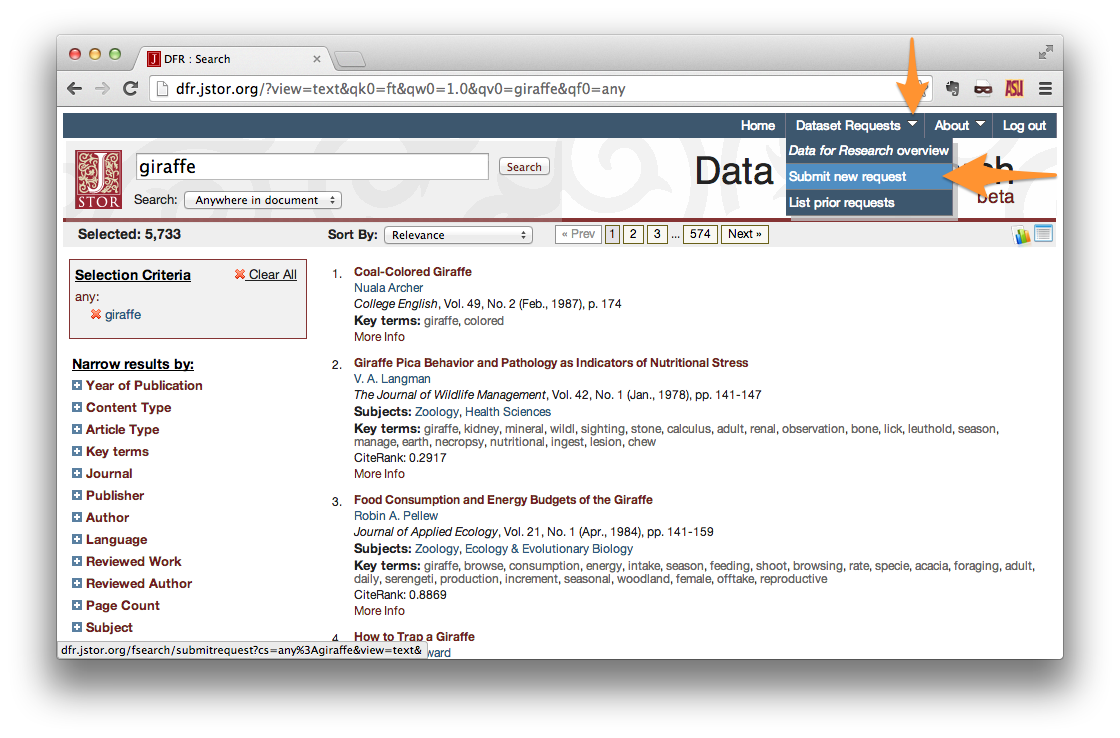
\includegraphics[width=0.600\linewidth]{getting.5.png}

On the \textbf{Download Options} page, select your desired \textbf{Data Type}. If you do not intend
to make use of the contents of the papers themselves, then ``Citations Only'' is sufficient.
Otherwise, choose word counts, bigrams, etc.

\textbf{Output Format} should be set to \textbf{XML}.

Give your request a title, and set the maximum number of articles. \emph{Note that the maximum
documents allowed per request is 1,000. Setting **Maximum Articles*} to a value less than
the number of search results will yield a random sample of your results.*

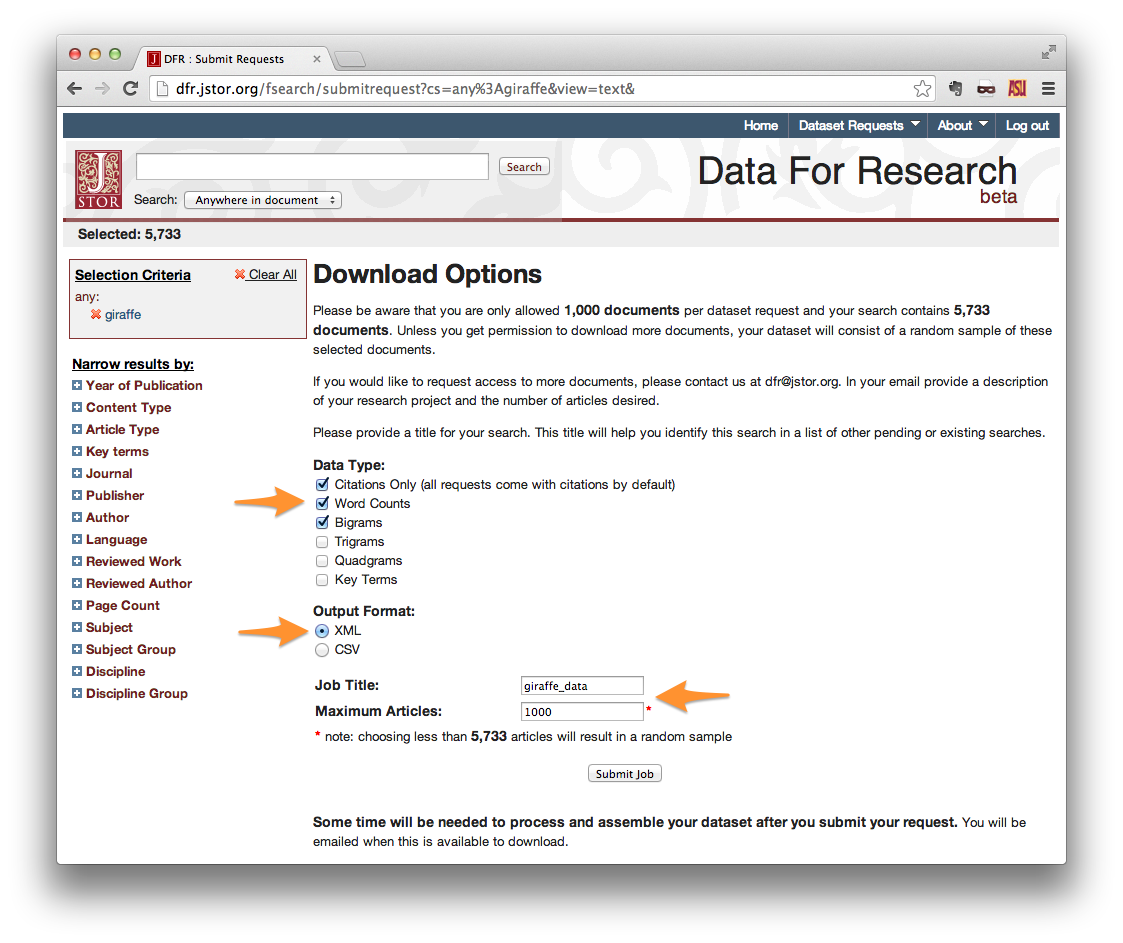
\includegraphics[width=0.600\linewidth]{getting.6.png}

Your request should now appear in your list of \textbf{Data Requests}. When your request is
ready (hours to days later), you will receive an e-mail with a download link. When
downloading from the \textbf{Data Requests} list, be sure to use the link in the
\textbf{full dataset} column.

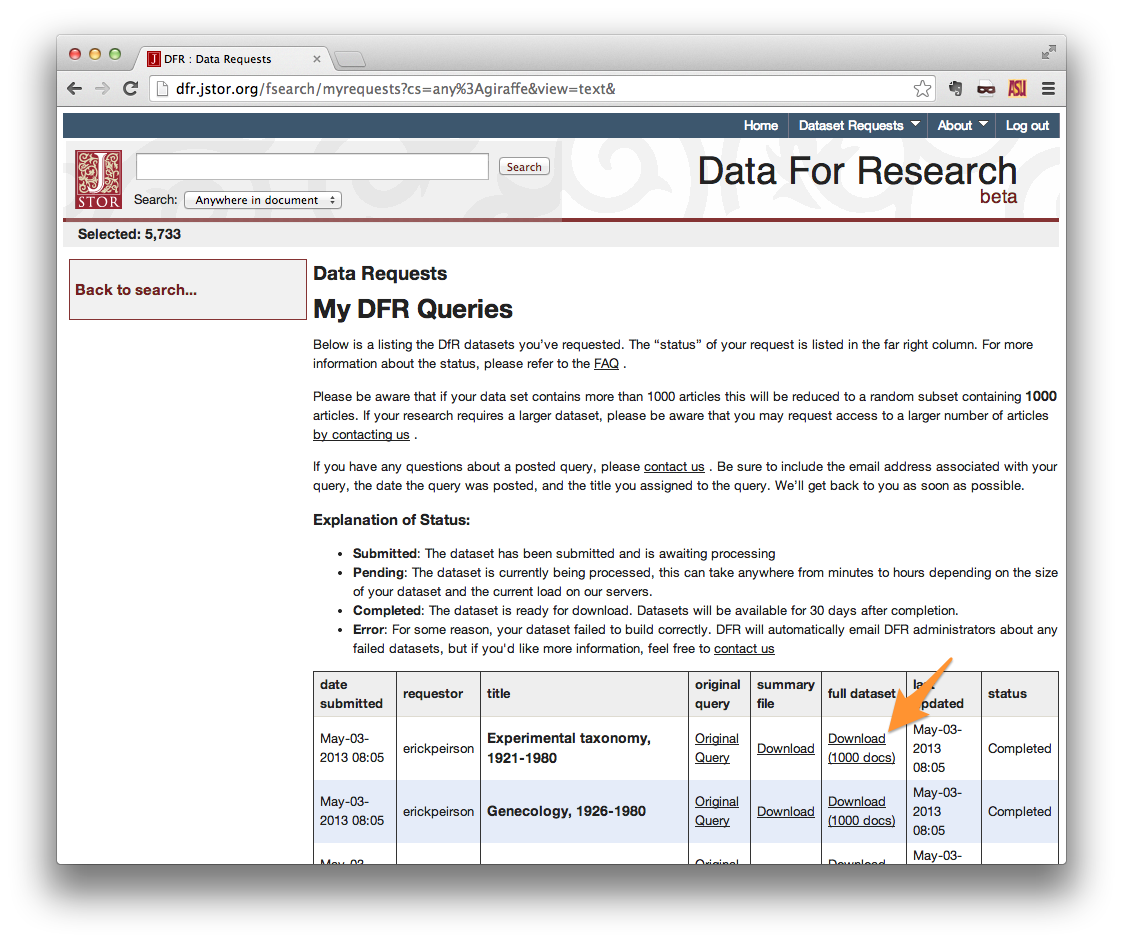
\includegraphics[width=0.600\linewidth]{getting.7.png}

When your dataset download is complete, unzip it. The contents should look something like
those shown below.

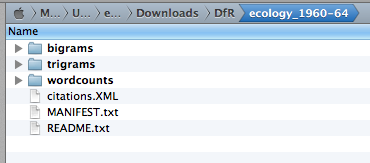
\includegraphics[width=0.400\linewidth]{getting.8.png}

\code{citations.XML} contains bibliographic data in XML format. The \code{bigrams}, \code{trigrams},
\code{wordcounts} folders contain N-gram counts for each document.

In the example above, the path this dataset is
\emph{/Users/erickpeirson/Downloads/DfR/ecology\_1960-64}. This is the path used in
{\hyperref[tethne.readers.dfr:tethne.readers.dfr.read]{\code{tethne.readers.dfr.read()}}} .


\subsubsection{Scopus}
\label{tutorial.getting_data:scopus}
As of v0.6.0-beta, Tethne supports data from the \href{http://www.elsevier.com/online-tools/scopus}{Scopus} bibliographic database.

For information about loading Scopus data in Tethne, see the {\hyperref[tethne.readers.scopus:module-tethne.readers.scopus]{\code{readers.scopus}}}
module.

Perform your search without whatever parameters you prefer. In this example, we are
searching for documents with \code{phenotypic} or \code{plasticity} in their titles, abstracts,
or keywords, and we're searching all available data in Scopus.

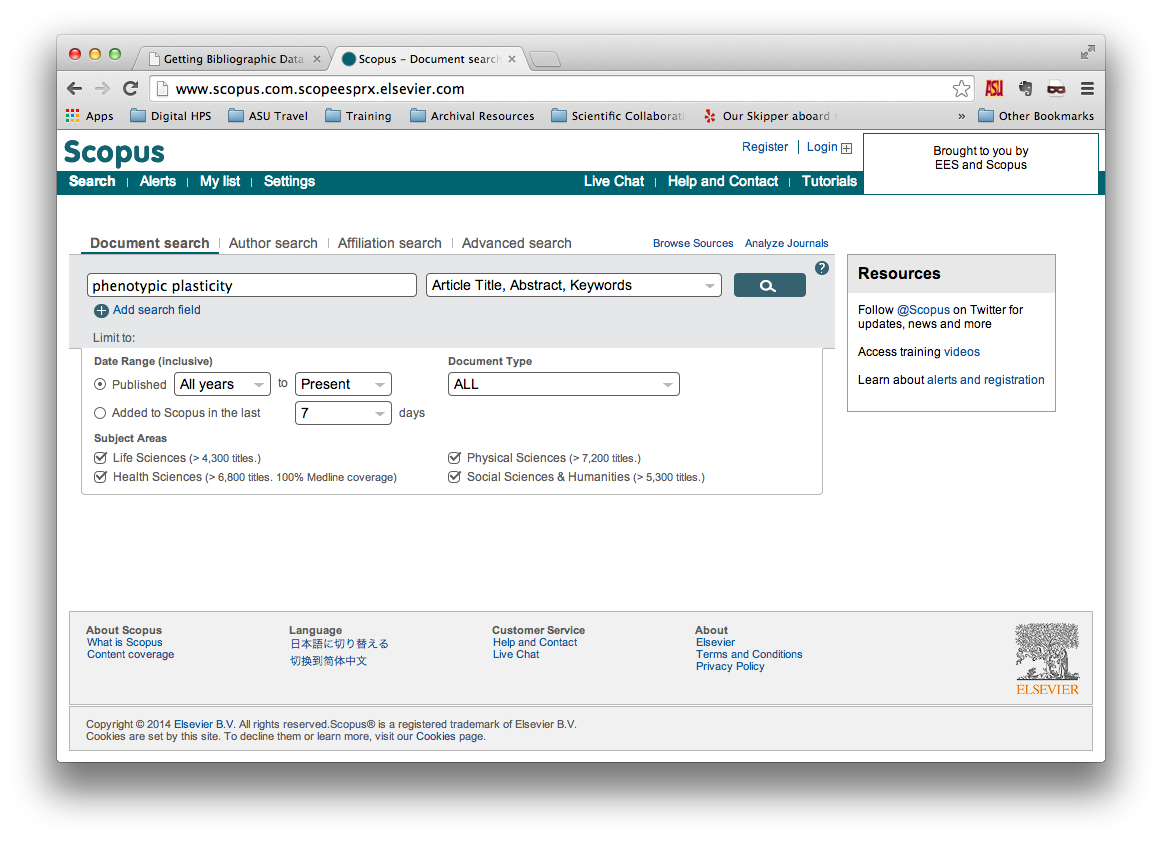
\includegraphics[width=0.600\linewidth]{getting.9.png}

From the search results page, select the records that you wish to export using the
checkboxes at left. Then click on ``Export'', just above the search results. This should
open a menu that looks similar to the one shown below.

Be sure to select the following:

\textbf{File type}: CSV
\textbf{Information to export}: All available information

Then click the ``Export'' button in the bottom right.

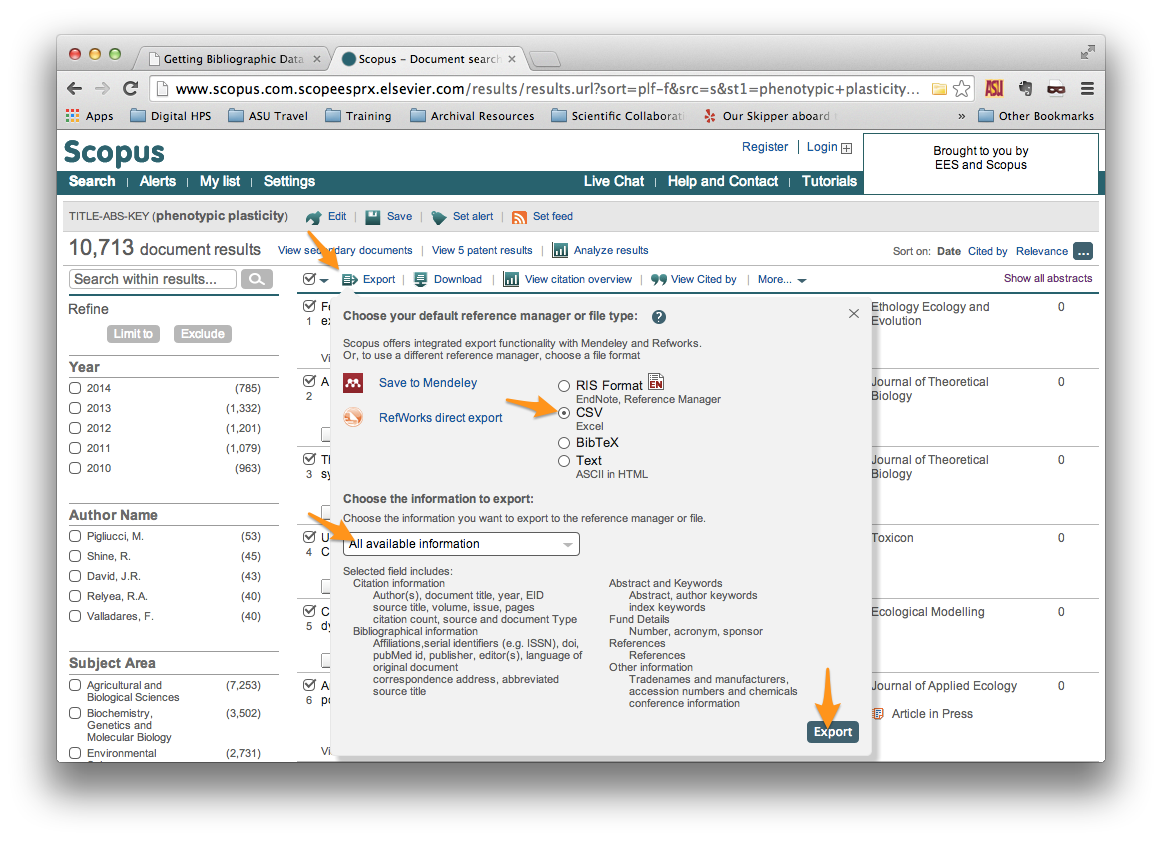
\includegraphics[width=0.600\linewidth]{getting.10.png}

After a few moments, your browser should begin downloading a file called \code{scopus.csv}.
If you were to open that file in your favorite spreadsheet application, the contents
should look something like what is shown below.

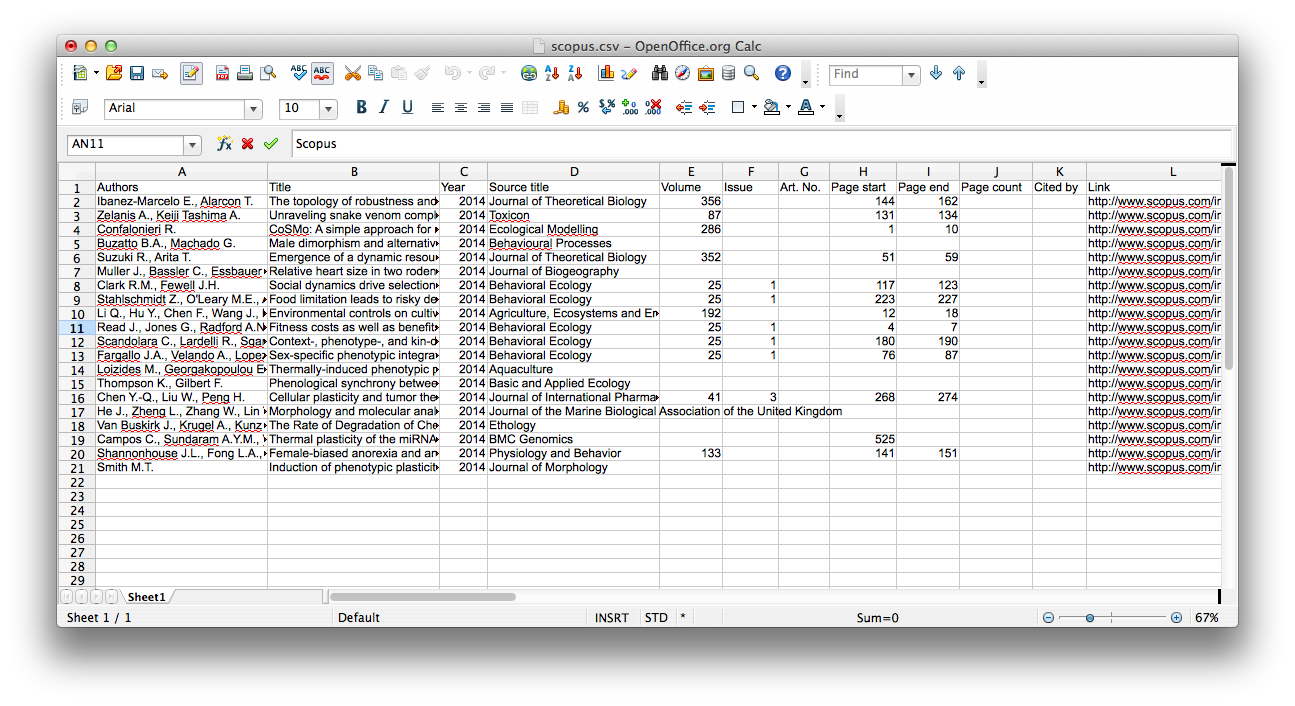
\includegraphics[width=0.600\linewidth]{getting.11.png}


\subsection{Working with Corpora}
\label{corpora::doc}\label{corpora:working-with-corpora}\label{corpora:id1}
Building a {\hyperref[tethne.classes.corpus:tethne.classes.corpus.Corpus]{\code{Corpus}}} is the starting-point for working with bibliographic data
in Tethne. {\hyperref[tethne.classes.corpus:tethne.classes.corpus.Corpus]{\code{Corpus}}} objects encapsulate and index {\hyperref[tethne.classes.paper:tethne.classes.paper.Paper]{\code{Paper}}}s and
{\hyperref[corpora:corpora-featuresets]{\emph{Featuresets}}}, and mechanisms for analyzing data diachronically.

The {\hyperref[tethne.classes.corpus:tethne.classes.corpus.Corpus]{\code{Corpus}}} class lives in {\hyperref[tethne.classes:module-tethne.classes]{\code{tethne.classes}}}, but can be imported directly
from {\hyperref[tethne:module-tethne]{\code{tethne}}}:

\begin{Verbatim}[commandchars=\\\{\}]
\PYG{g+gp}{\PYGZgt{}\PYGZgt{}\PYGZgt{} }\PYG{k+kn}{from} \PYG{n+nn}{tethne} \PYG{k+kn}{import} \PYG{n}{Corpus}
\end{Verbatim}


\subsubsection{Creating Corpora}
\label{corpora:creating-corpora}
Minimally, a {\hyperref[tethne.classes.corpus:tethne.classes.corpus.Corpus]{\code{Corpus}}} requires a set of {\hyperref[tethne.classes.paper:tethne.classes.paper.Paper]{\code{Paper}}}s.

\begin{Verbatim}[commandchars=\\\{\}]
\PYG{g+gp}{\PYGZgt{}\PYGZgt{}\PYGZgt{} }\PYG{k+kn}{from} \PYG{n+nn}{tethne.readers} \PYG{k+kn}{import} \PYG{n}{wos}
\PYG{g+gp}{\PYGZgt{}\PYGZgt{}\PYGZgt{} }\PYG{n}{papers} \PYG{o}{=} \PYG{n}{wos}\PYG{o}{.}\PYG{n}{read}\PYG{p}{(}\PYG{l+s}{\PYGZsq{}}\PYG{l+s}{/path/to/wosdata.txt}\PYG{l+s}{\PYGZsq{}}\PYG{p}{)}    \PYG{c}{\PYGZsh{} Load some data.}

\PYG{g+gp}{\PYGZgt{}\PYGZgt{}\PYGZgt{} }\PYG{n}{MyCorpus} \PYG{o}{=} \PYG{n}{Corpus}\PYG{p}{(}\PYG{n}{papers}\PYG{p}{)}
\end{Verbatim}


\paragraph{Indexing}
\label{corpora:indexing}
By default, {\hyperref[tethne.classes.paper:tethne.classes.paper.Paper]{\code{Paper}}}s and their cited references are indexed by `ayjid', an
identifier generated from the first-author, publication date, and journal name of each
entry.

You can use alternate indexing fields for {\hyperref[tethne.classes.paper:tethne.classes.paper.Paper]{\code{Paper}}}s and their cited references:

\begin{Verbatim}[commandchars=\\\{\}]
\PYG{g+gp}{\PYGZgt{}\PYGZgt{}\PYGZgt{} }\PYG{n}{MyCorpus} \PYG{o}{=} \PYG{n}{Corpus}\PYG{p}{(}\PYG{n}{papers}\PYG{p}{,} \PYG{n}{index\PYGZus{}by}\PYG{o}{=}\PYG{l+s}{\PYGZsq{}}\PYG{l+s}{wosid}\PYG{l+s}{\PYGZsq{}}\PYG{p}{,} \PYG{n}{index\PYGZus{}citation\PYGZus{}by}\PYG{o}{=}\PYG{l+s}{\PYGZsq{}}\PYG{l+s}{ayjid}\PYG{l+s}{\PYGZsq{}}\PYG{p}{)}
\end{Verbatim}

These are (usually) your options for index fields for \code{Papers} (\code{index\_by}):

\begin{tabulary}{\linewidth}{|L|L|}
\hline
\textsf{\relax 
Source
} & \textsf{\relax 
Fields
}\\
\hline
Web of Science
 & 
wosid, ayjid
\\

Scopus
 & 
eid, ayjid
\\

JSTOR DfR
 & 
doi, ayjid
\\
\hline\end{tabulary}


It should be obvious that \code{ayjid} is a good option if you plan to integrate data from
multiple datasources. \code{ayjid} is your best option for \code{index\_citations\_by}, unless
you're confident that all cited references include alternate identifiers (this is rare).

By default, a {\hyperref[tethne.classes.corpus:tethne.classes.corpus.Corpus]{\code{Corpus}}} calls its own \code{Corpus.index()} method on instantiation.
This results in a few useful attributes:

\begin{tabulary}{\linewidth}{|L|L|}
\hline
\textsf{\relax 
Attribute
} & \textsf{\relax 
Type/Description
}\\
\hline
papers
 & 
A dictionary mapping {\hyperref[tethne.classes.paper:tethne.classes.paper.Paper]{\code{Paper}}} IDs onto {\hyperref[tethne.classes.paper:tethne.classes.paper.Paper]{\code{Paper}}}
instances.
\\

authors
 & 
A dictionary mapping author names onto lists of {\hyperref[tethne.classes.paper:tethne.classes.paper.Paper]{\code{Paper}}} IDs.
\\

citations
 & 
A dictionary mapping citation IDs onto cited references (themselves
{\hyperref[tethne.classes.paper:tethne.classes.paper.Paper]{\code{Paper}}} instances), if data available.
\\

papers\_citing
 & 
A dictionary mapping citation IDs onto lists of citing
{\hyperref[tethne.classes.paper:tethne.classes.paper.Paper]{\code{Paper}}}s (by ID) in the dataset, if data available.
\\
\hline\end{tabulary}


If the {\hyperref[tethne.classes.paper:tethne.classes.paper.Paper]{\code{Paper}}}s in the {\hyperref[tethne.classes.corpus:tethne.classes.corpus.Corpus]{\code{Corpus}}} contain cited references, then a
featureset called \code{citations} will also be created.


\paragraph{Directly from data}
\label{corpora:directly-from-data}
All of the modules in {\hyperref[tethne.readers:module-tethne.readers]{\code{readers}}} should include methods to generate a
{\hyperref[tethne.classes.corpus:tethne.classes.corpus.Corpus]{\code{Corpus}}} directly from data:
\begin{itemize}
\item {} 
{\hyperref[tethne.readers.dfr:tethne.readers.dfr.read_corpus]{\code{dfr.read\_corpus()}}}

\item {} 
{\hyperref[tethne.readers.scopus:tethne.readers.scopus.read_corpus]{\code{scopus.read\_corpus()}}}

\item {} 
{\hyperref[tethne.readers.wos:tethne.readers.wos.read_corpus]{\code{wos.read\_corpus()}}}

\end{itemize}


\subsubsection{Featuresets}
\label{corpora:corpora-featuresets}\label{corpora:featuresets}
In Tethne, a feature is a scalar property of one or more document in a {\hyperref[tethne.classes.corpus:tethne.classes.corpus.Corpus]{\code{Corpus}}}.
The most straightforward example of a feature is a word, which can occur some number of
times ( \textgreater{}= 0 ) in a document.

A featureset is a set of data structures that describe the distribution of features
over {\hyperref[tethne.classes.paper:tethne.classes.paper.Paper]{\code{Paper}}}s in a corpus. For example, a {\hyperref[tethne.classes.corpus:tethne.classes.corpus.Corpus]{\code{Corpus}}} might contain a
featureset describing the distribution of words or citations over its {\hyperref[tethne.classes.paper:tethne.classes.paper.Paper]{\code{Paper}}}s.

In Tethne v0.6.0-beta, featuresets are simply dictionaries contained in the
{\hyperref[tethne.classes.corpus:tethne.classes.corpus.Corpus]{\code{Corpus}}}` \code{features} attribute. Each featureset should contain the following
keys and values:

\begin{tabulary}{\linewidth}{|L|L|}
\hline
\textsf{\relax 
Key
} & \textsf{\relax 
Value Type/Description
}\\
\hline
\code{index}
 & 
Dictionary mapping integer IDs onto string representations of
features. For wordcounts, think of this as a vocabulary.
\\

\code{features}
 & 
Dictionary mapping {\hyperref[tethne.classes.paper:tethne.classes.paper.Paper]{\code{Paper}}} IDs onto sparse feature vectors
(e.g. wordcounts). These vectors are lists of ( feature index,
value ) tuples.
\\

\code{counts}
 & 
Dictionary mapping feature indices (in \code{index}) onto the sum of
values from \code{features}. For wordcounts, for example, this is the
total number of times that a word occurs in the {\hyperref[tethne.classes.corpus:tethne.classes.corpus.Corpus]{\code{Corpus}}}.
\\

\code{documentCounts}
 & 
Dictionary mapping feature indices (in \code{index}) onto the number
of {\hyperref[tethne.classes.paper:tethne.classes.paper.Paper]{\code{Paper}}}s in which the feature occurs (e.g. the number
of documents containing that word).
\\
\hline\end{tabulary}


The following methods in {\hyperref[tethne.classes.corpus:tethne.classes.corpus.Corpus]{\code{Corpus}}} are useful for working with featuresets:

\begin{longtable}{ll}
\hline
\endfirsthead

\multicolumn{2}{c}%
{{\textsf{\tablename\ \thetable{} -- continued from previous page}}} \\
\hline
\endhead

\hline \multicolumn{2}{|r|}{{\textsf{Continued on next page}}} \\ \hline
\endfoot

\endlastfoot


{\hyperref[tethne.classes.corpus:tethne.classes.corpus.Corpus.abstract_to_features]{\code{Corpus.abstract\_to\_features}}}
 & 

\\

{\hyperref[tethne.classes.corpus:tethne.classes.corpus.Corpus.add_features]{\code{Corpus.add\_features}}}
 & 

\\

{\hyperref[tethne.classes.corpus:tethne.classes.corpus.Corpus.apply_stoplist]{\code{Corpus.apply\_stoplist}}}
 & 

\\

{\hyperref[tethne.classes.corpus:tethne.classes.corpus.Corpus.feature_counts]{\code{Corpus.feature\_counts}}}
 & 

\\

{\hyperref[tethne.classes.corpus:tethne.classes.corpus.Corpus.feature_distribution]{\code{Corpus.feature\_distribution}}}
 & 

\\

{\hyperref[tethne.classes.corpus:tethne.classes.corpus.Corpus.filter_features]{\code{Corpus.filter\_features}}}
 & 

\\

{\hyperref[tethne.classes.corpus:tethne.classes.corpus.Corpus.plot_distribution]{\code{Corpus.plot\_distribution}}}
 & 

\\

{\hyperref[tethne.classes.corpus:tethne.classes.corpus.Corpus.transform]{\code{Corpus.transform}}}
 & 

\\
\hline\end{longtable}



\subsection{Bibliographic Coupling}
\label{tutorial.bibliocoupling::doc}\label{tutorial.bibliocoupling:bibliographic-coupling}\setbox0\vbox{
\begin{minipage}{0.95\linewidth}
\begin{itemize}
\item {} 
{\hyperref[tutorial.bibliocoupling:getting-started]{Getting Started}}

\item {} 
{\hyperref[tutorial.bibliocoupling:reading-wos-data]{Reading WoS Data}}

\item {} 
{\hyperref[tutorial.bibliocoupling:building-a-static-network]{Building a Static Network}}

\item {} 
{\hyperref[tutorial.bibliocoupling:export-to-graphml]{Export to GraphML}}

\item {} 
{\hyperref[tutorial.bibliocoupling:visualizing-static-networks-in-cytoscape]{Visualizing Static Networks in Cytoscape}}
\begin{itemize}
\item {} 
{\hyperref[tutorial.bibliocoupling:import]{Import}}

\item {} 
{\hyperref[tutorial.bibliocoupling:cluster-detection]{Cluster Detection}}

\end{itemize}

\item {} 
{\hyperref[tutorial.bibliocoupling:evolving-networks]{Evolving Networks}}
\begin{itemize}
\item {} 
{\hyperref[tutorial.bibliocoupling:slicing-a-corpus]{Slicing a Corpus}}

\item {} 
{\hyperref[tutorial.bibliocoupling:building-a-graphcollection]{Building a GraphCollection}}

\end{itemize}

\item {} 
{\hyperref[tutorial.bibliocoupling:visualizing-a-dynamic-network]{Visualizing a Dynamic Network}}

\end{itemize}
\end{minipage}}
\begin{center}\setlength{\fboxsep}{5pt}\shadowbox{\box0}\end{center}

Bibliographic coupling can be a useful and computationally cheap way to explore the
thematic topology of a large scientific literature.

\href{http://en.wikipedia.org/wiki/Bibliographic\_coupling}{Bibliographic coupling} was first
proposed as a method for detecting latent topical affinities among research publications
by Myer M. Kessler at MIT in 1958. In 1972, J.C. Donohue suggested that bibliographic
coupling could be used to the map ``research fronts'' in science, and this method, along
with co-citation analysis and other citation-based clustering techniques, became a core
methodology of the science-mapping craze of the 1970s. Bibliographic coupling is still
employed in the context of both information-retrieval and science-studies.

Two papers are bibliographically coupled if they both cite at least some of the same
papers. The core assumption of bibliographic coupling analysis is that if two papers
cite similar literatures, then they must be topically related in some way. That is, they
are more likely to be related to each other than to papers with which they share no cited
references.

{\hfill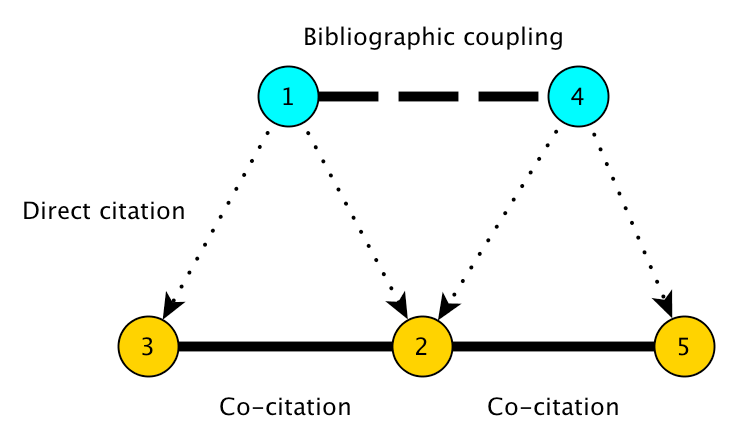
\includegraphics{citationnetworks.png}\hfill}

This tutorial provides a walk-through for building bibliographic coupling networks from
Web of Science citation data. What we are aiming for is a graph model of our bibliographic
data that reveals thematically coherent and informative clusters of documents. We will use
Tethne's \code{bibligraphic\_coupling()} method, along with Cytocape's MCODE clustering
plugin, to generate a visualization that looks something like this:

{\hfill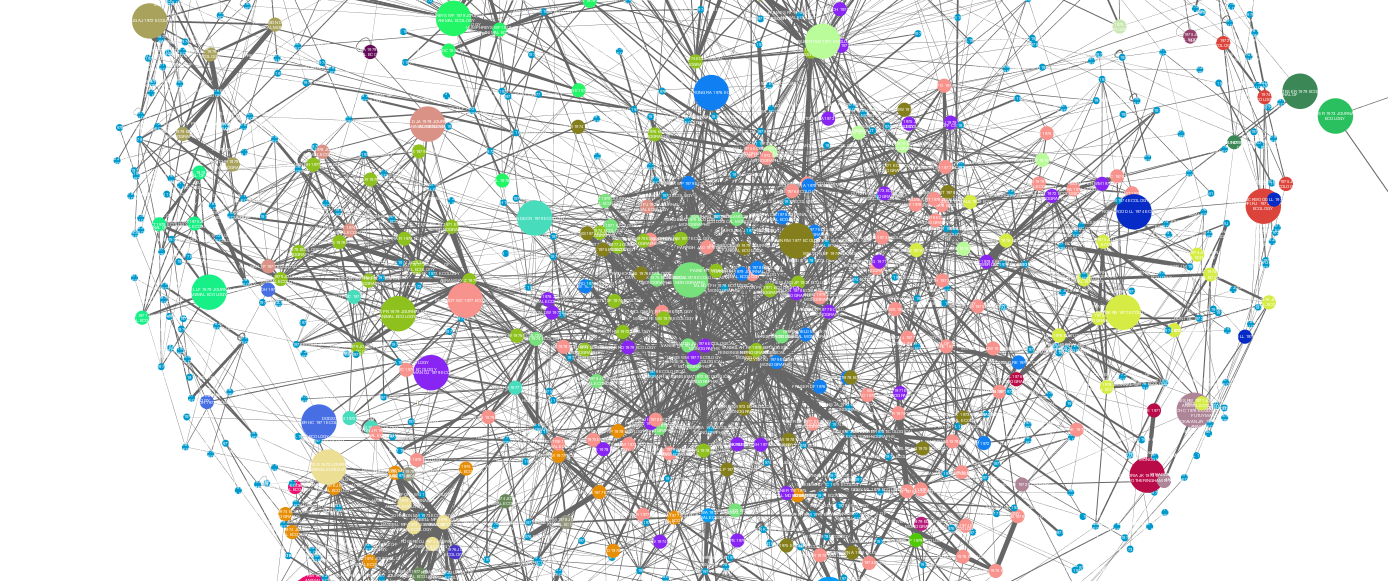
\includegraphics{bibliographic_coupling.png}\hfill}

In this example, each node represents a scientific paper, and each densely-connected
colored group of nodes corresponds to a research theme or sub-field that holds those
papers together.


\subsubsection{Getting Started}
\label{tutorial.bibliocoupling:getting-started}
Before you begin, be sure to install the latest version of Tethne. Consult the
\emph{installation} guide for details.

\textbf{If you run into problems}, don't panic. Tethne is under active development, and there
are certainly bugs to be found. Please report any problems, including errors in this
tutorial, via our \href{https://github.com/diging/tethne/issues?state=open}{GitHub issue tracker}.

For this tutorial, you'll need some citation data from the ISI Web of Science. If this is
your first time working with WoS citation data, check out {\hyperref[tutorial.getting_data:gettingdata]{\emph{Getting Bibliographic Data}}}. We'll
assume that you have downloaded a few sets of records from WoS, and stored them all in
the same directory.

\begin{Verbatim}[commandchars=\\\{\}]
\PYG{g+gp}{\PYGZgt{}\PYGZgt{}\PYGZgt{} }\PYG{n}{datapath} \PYG{o}{=} \PYG{l+s}{\PYGZsq{}}\PYG{l+s}{/path/to/my/data/directory}\PYG{l+s}{\PYGZsq{}}
\end{Verbatim}


\subsubsection{Reading WoS Data}
\label{tutorial.bibliocoupling:reading-wos-data}
You can parse WoS data from one or multiple field-tagged data files, using the methods
in the {\hyperref[tethne.readers:module-tethne.readers]{\code{readers}}} module. Since we're working with multiple data files, we'll
use the \code{readers.wos.corpus\_from\_dir} method to parse the WoS data and create
a new {\hyperref[tethne.classes.corpus:tethne.classes.corpus.Corpus]{\code{Corpus}}} called \code{MyCorpus}.

\begin{Verbatim}[commandchars=\\\{\}]
\PYG{g+gp}{\PYGZgt{}\PYGZgt{}\PYGZgt{} }\PYG{k+kn}{from} \PYG{n+nn}{tethne.readers} \PYG{k+kn}{import} \PYG{n}{wos}
\PYG{g+gp}{\PYGZgt{}\PYGZgt{}\PYGZgt{} }\PYG{n}{MyCorpus} \PYG{o}{=} \PYG{n}{wos}\PYG{o}{.}\PYG{n}{corpus\PYGZus{}from\PYGZus{}dir}\PYG{p}{(}\PYG{n}{datapath}\PYG{p}{)}
\end{Verbatim}

\code{MyCorpus} should contain some {\hyperref[tethne.classes.paper:tethne.classes.paper.Paper]{\code{Paper}}}s, as well as some citations.

\begin{Verbatim}[commandchars=\\\{\}]
\PYG{g+gp}{\PYGZgt{}\PYGZgt{}\PYGZgt{} }\PYG{k}{print} \PYG{n+nb}{len}\PYG{p}{(}\PYG{n}{MyCorpus}\PYG{o}{.}\PYG{n}{papers}\PYG{p}{)}       \PYG{c}{\PYGZsh{} How many Papers?}
\PYG{g+go}{1859}
\PYG{g+gp}{\PYGZgt{}\PYGZgt{}\PYGZgt{} }\PYG{k}{print} \PYG{n+nb}{len}\PYG{p}{(}\PYG{n}{MyCorpus}\PYG{o}{.}\PYG{n}{citations}\PYG{p}{)}    \PYG{c}{\PYGZsh{} How many citations?}
\PYG{g+go}{57774}
\end{Verbatim}

If you have fewer {\hyperref[tethne.classes.paper:tethne.classes.paper.Paper]{\code{Paper}}}s than you expect, it is possible that some of the
records in your dataset were duplicates. If you don't have any citations, go back
and make sure that you downloaded full records with citations from the WoS database. See
{\hyperref[tutorial.getting_data:gettingdata]{\emph{Getting Bibliographic Data}}}.


\subsubsection{Building a Static Network}
\label{tutorial.bibliocoupling:building-a-static-network}
We will first build a static bibliographic coupling network using all of the
{\hyperref[tethne.classes.paper:tethne.classes.paper.Paper]{\code{Paper}}}s in our {\hyperref[tethne.classes.corpus:tethne.classes.corpus.Corpus]{\code{Corpus}}}. To create a static network, we can use the
methods in {\hyperref[tethne.networks:module-tethne.networks]{\code{networks}}} directly. The {\hyperref[tethne.networks.papers:tethne.networks.papers.bibliographic_coupling]{\code{bibliographic\_coupling()}}} method can be
found in the {\hyperref[tethne.networks.papers:module-tethne.networks.papers]{\code{networks.papers}}} module.

\begin{Verbatim}[commandchars=\\\{\}]
\PYG{g+gp}{\PYGZgt{}\PYGZgt{}\PYGZgt{} }\PYG{k+kn}{from} \PYG{n+nn}{tethne.networks} \PYG{k+kn}{import} \PYG{n}{papers}
\PYG{g+gp}{\PYGZgt{}\PYGZgt{}\PYGZgt{} }\PYG{n}{bc\PYGZus{}network} \PYG{o}{=} \PYG{n}{papers}\PYG{o}{.}\PYG{n}{bibliographic\PYGZus{}coupling}\PYG{p}{(}\PYG{n}{MyCorpus}\PYG{o}{.}\PYG{n}{all\PYGZus{}papers}\PYG{p}{(}\PYG{p}{)}\PYG{p}{,} \PYG{n}{threshold}\PYG{o}{=}\PYG{l+m+mi}{3}\PYG{p}{)}
\end{Verbatim}

In the example above, the \code{Corpus.all\_papers()} method gets all of the papers from
\code{MyCorpus}. \code{threshold=3} means that two papers must share at least three
bibliographic references to be considered coupled.

Generating an informative graph using bibliographic coupling will require some tuning.
Depending on the criteria that you used to generate your bibliographic dataset, you may
need to adjust the coupling \code{threshold}. Papers from a relatively narrow field have a
high probability of sharing cited references, thus a threshold of \code{1} shared reference
will result in a nearly complete graph that yields little information about the latent
topical structure of that literature. If your dataset contains papers from quite disparate
fields, however, you may wish to keep the threshold low.

Since papers vary widely in the total number of references that they cite, it may be
desirable to use a normalized overlap value rather than an absolute one. If the
\code{weighted} parameter is set to \code{True}, Tethne will use the normalized similarity
metric \code{s}:
\begin{gather}
\begin{split}s = \frac{N_{i|j}}{\sqrt{ N_i N_j }}\end{split}\notag
\end{gather}
If you choose to use absolute overlap (\code{weighted} is \code{False}), we suggest starting
with a \code{threshold} of \code{5}, and then adjusting it upward or downward to achieve optimal
clustering. If you choose to use normalized overlap (\code{weighted} is \code{True}), then try
starting with a \code{threshold} of \code{0.05}.

We'll also include some node attributes: \code{date}, \code{jtitle} (journal title), and
\code{atitle} (article title).

\begin{Verbatim}[commandchars=\\\{\}]
\PYG{g+gp}{\PYGZgt{}\PYGZgt{}\PYGZgt{} }\PYG{k+kn}{from} \PYG{n+nn}{tethne.networks} \PYG{k+kn}{import} \PYG{n}{papers}
\PYG{g+gp}{\PYGZgt{}\PYGZgt{}\PYGZgt{} }\PYG{n}{bc\PYGZus{}network} \PYG{o}{=} \PYG{n}{papers}\PYG{o}{.}\PYG{n}{bibliographic\PYGZus{}coupling}\PYG{p}{(}\PYG{n}{MyCorpus}\PYG{o}{.}\PYG{n}{all\PYGZus{}papers}\PYG{p}{(}\PYG{p}{)}\PYG{p}{,} \PYG{n}{threshold}\PYG{o}{=}\PYG{l+m+mf}{0.05}\PYG{p}{,}
\PYG{g+gp}{... }    \PYG{n}{node\PYGZus{}attribs}\PYG{o}{=}\PYG{p}{[}\PYG{l+s}{\PYGZsq{}}\PYG{l+s}{date}\PYG{l+s}{\PYGZsq{}}\PYG{p}{,} \PYG{l+s}{\PYGZsq{}}\PYG{l+s}{jtitle}\PYG{l+s}{\PYGZsq{}}\PYG{p}{,} \PYG{l+s}{\PYGZsq{}}\PYG{l+s}{atitle}\PYG{l+s}{\PYGZsq{}}\PYG{p}{]}\PYG{p}{,} \PYG{n}{weighted}\PYG{o}{=}\PYG{n+nb+bp}{True}\PYG{p}{)}
\end{Verbatim}


\subsubsection{Export to GraphML}
\label{tutorial.bibliocoupling:export-to-graphml}
\href{http://graphml.graphdrawing.org}{GraphML} is a widely-used static network data format.
We will write our network to GraphML for visualization in Cytoscape.

This step should generate a file in your output folder called
\code{{[}DATASET\_ID{]}\_graph\_all.graphml}.

{\hfill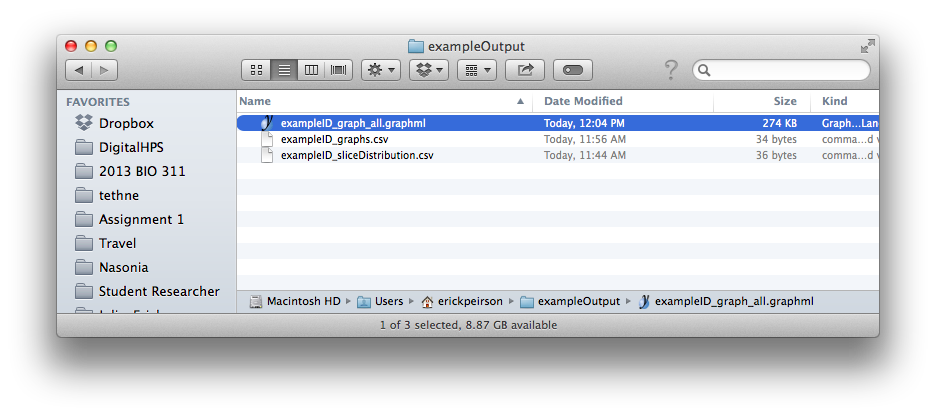
\includegraphics{coauthors.6.png}\hfill}

Use the {\hyperref[tethne.writers.graph:tethne.writers.graph.to_graphml]{\code{to\_graphml()}}} method in {\hyperref[tethne.writers.graph:module-tethne.writers.graph]{\code{writers.graph}}} to create a GraphML
data file.

\begin{Verbatim}[commandchars=\\\{\}]
\PYG{g+gp}{\PYGZgt{}\PYGZgt{}\PYGZgt{} }\PYG{k+kn}{from} \PYG{n+nn}{tethne.writers} \PYG{k+kn}{import} \PYG{n}{graph}
\PYG{g+gp}{\PYGZgt{}\PYGZgt{}\PYGZgt{} }\PYG{n}{graph}\PYG{o}{.}\PYG{n}{to\PYGZus{}graphml}\PYG{p}{(}\PYG{n}{bc\PYGZus{}network}\PYG{p}{,} \PYG{l+s}{\PYGZsq{}}\PYG{l+s}{/path/to/my/bc\PYGZus{}network.graphml}\PYG{l+s}{\PYGZsq{}}\PYG{p}{)}
\end{Verbatim}

In the example above, a new file called \code{bc\_network.graphml} should be created in
the \code{/path/to/my} directory.


\subsubsection{Visualizing Static Networks in Cytoscape}
\label{tutorial.bibliocoupling:visualizing-static-networks-in-cytoscape}
Cytoscape was developed in 2002, with funding from the National Instute of General Medical
Sciences and the National Resource for Network Biology. The primary user base is the
biomedical research community, especially systems biologists who study gene or protein
interaction networks and pathways.

You can download Cytoscape 3 from \href{http://www.cytoscape.org}{http://www.cytoscape.org}.
In this tutorial we are using Cytoscape 3.1.


\paragraph{Import}
\label{tutorial.bibliocoupling:import}
In Cytoscape, import your network by selecting \code{File \textgreater{} Import \textgreater{} Network \textgreater{} From file...}
and selecting the GraphML file generated by Tethne in your output directory.

Tethne includes the \code{similarity} of each pair of papers as an edge attribute. You can
tell Cytoscape to take similarity into account when laying out your graph. To apply an
edge-weighted layout, select \code{Layout \textgreater{} Edge-weighted Spring Embedded \textgreater{} similarity}.

{\hfill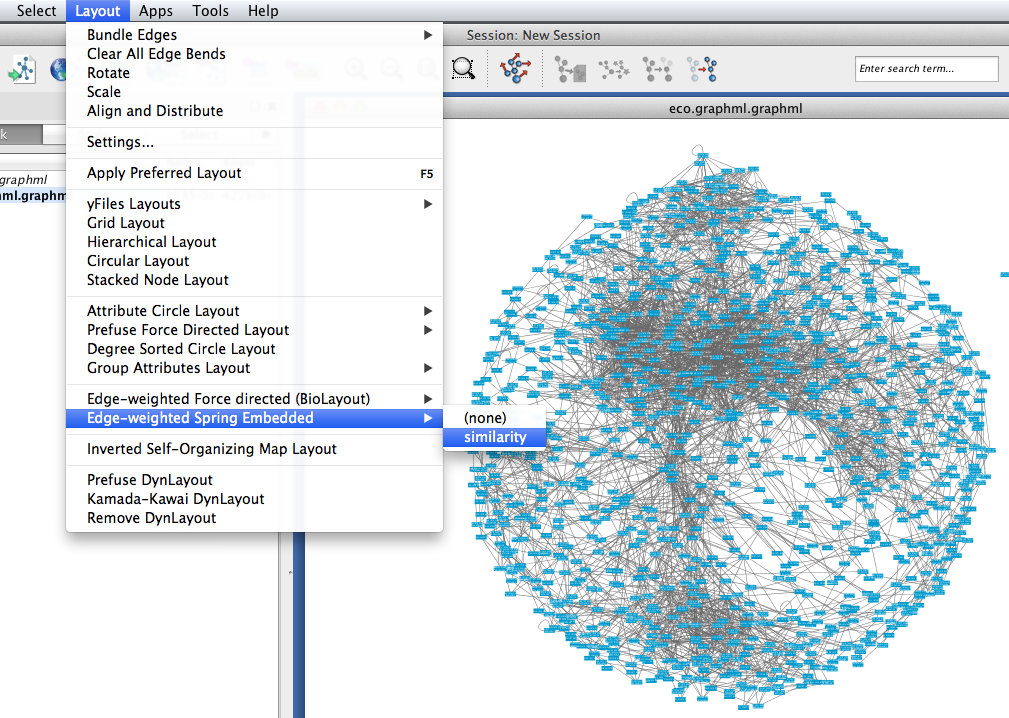
\includegraphics{cyto.1.png}\hfill}

Your network may look like a giant hairball. If you can't see much structure at all, you
may wish to go back and rebuild the graph with a higher threshold. If your network is very
sparse, you may wish to lower the threshold.

Set edge weight as a function of \code{similarity} to see which links are the strongest in
your network.

{\hfill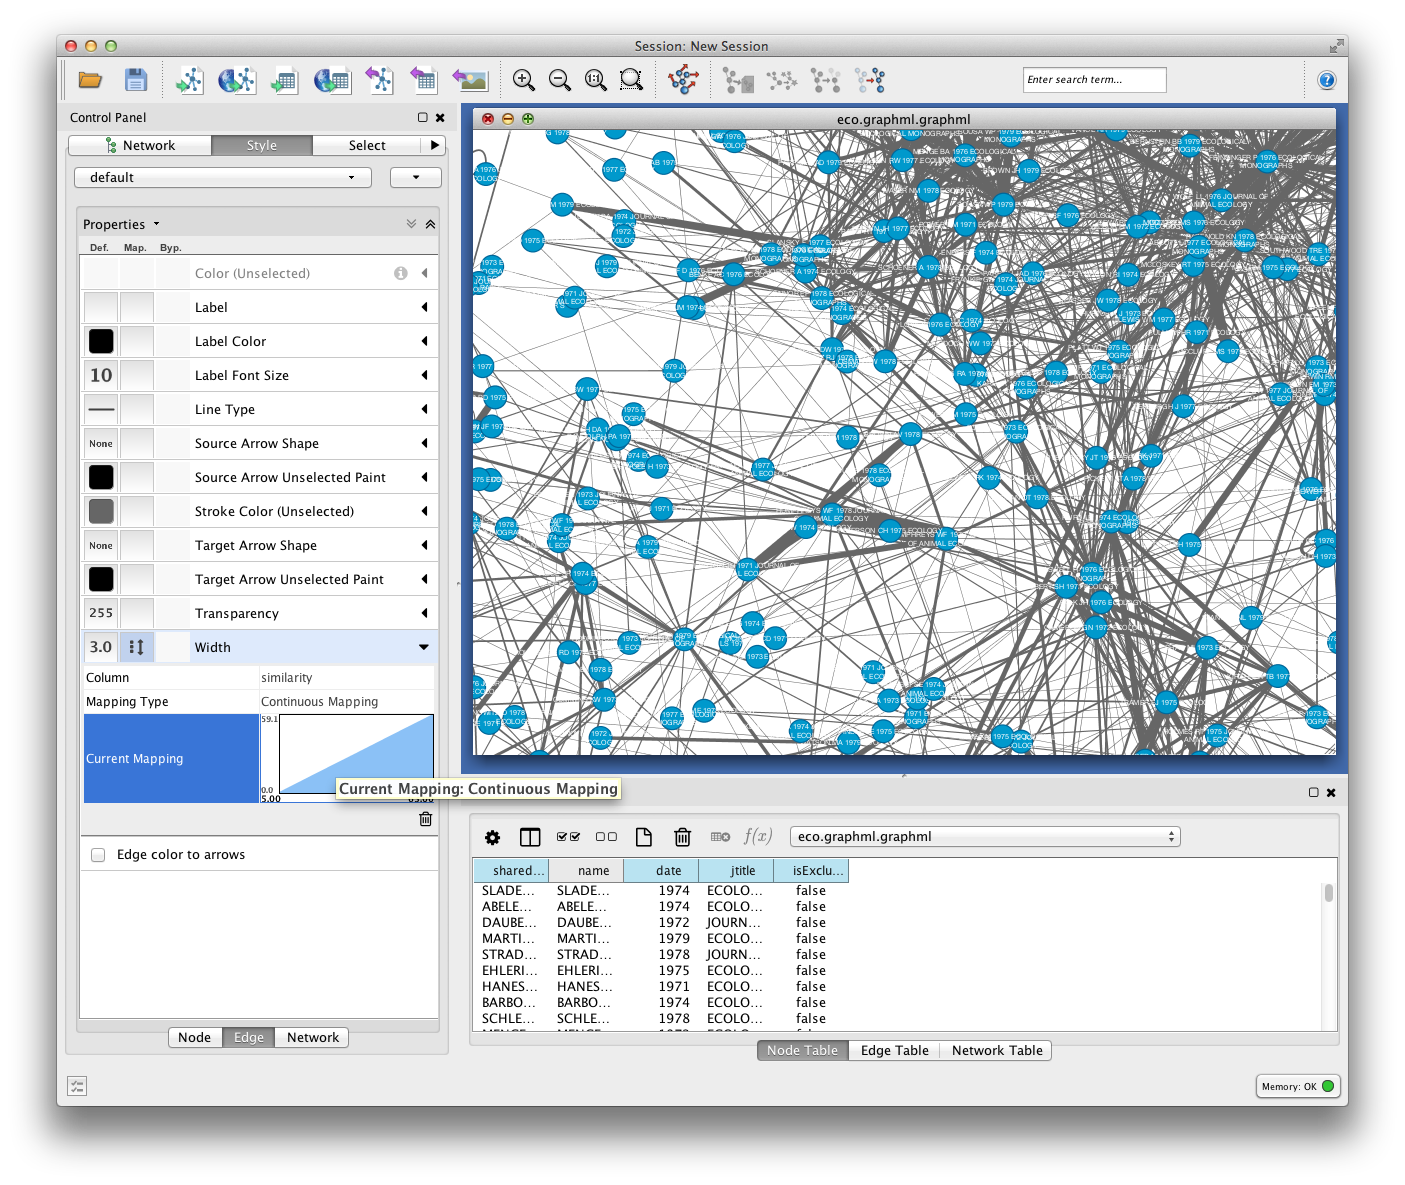
\includegraphics{cyto.2.png}\hfill}

To get some idea of whether certain clusters in the network correspond to publication
in the same journal, set node fill color as a discrete function of \code{jtitle}. You can
automatically generate node fill colors by right-clicking on the visual mapping, and
selecting \code{Mapping Value Generators \textgreater{} Random Color}.

{\hfill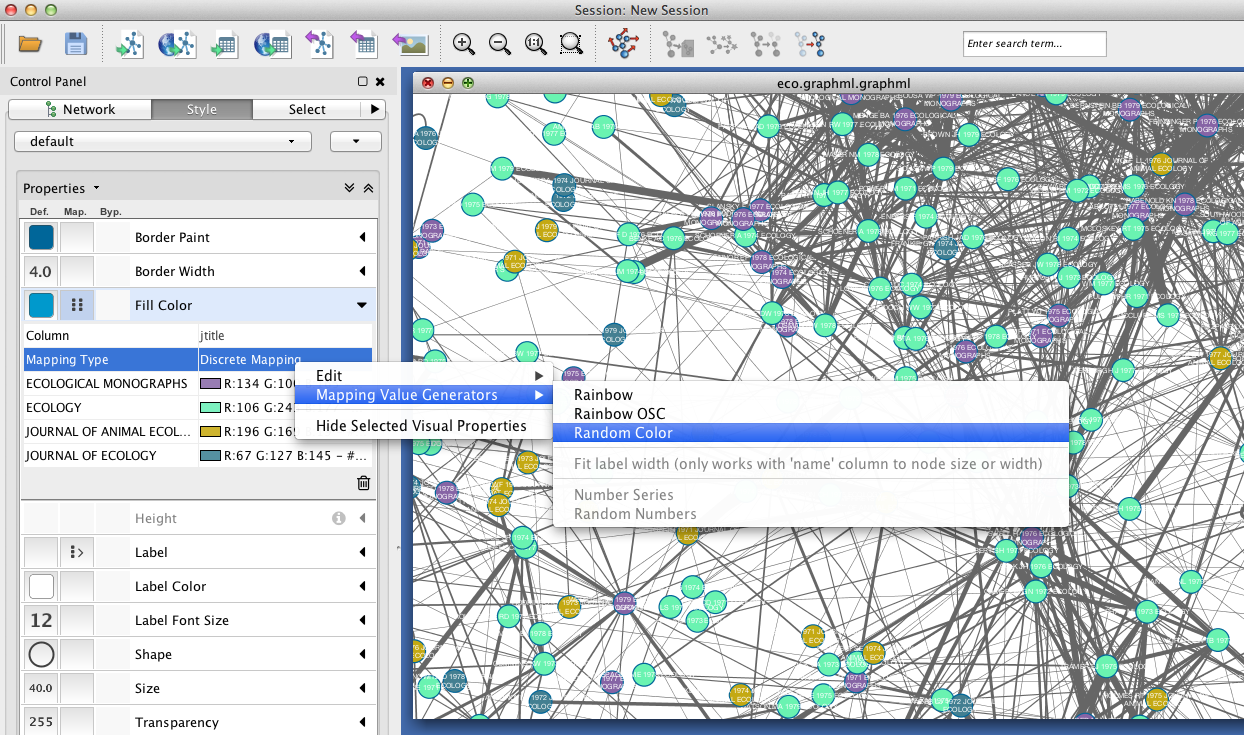
\includegraphics{cyto.3.png}\hfill}

Since you included the title of each paper (\code{atitle}) as a node attribute, you can
get some idea of what makes a particular region of the network hang together by selecting
some nodes and inspecting the \code{Node Table} in the \code{Table Panel}. In the example below,
a quick visual inspection suggests that parasites figure heavily in the selected papers.

{\hfill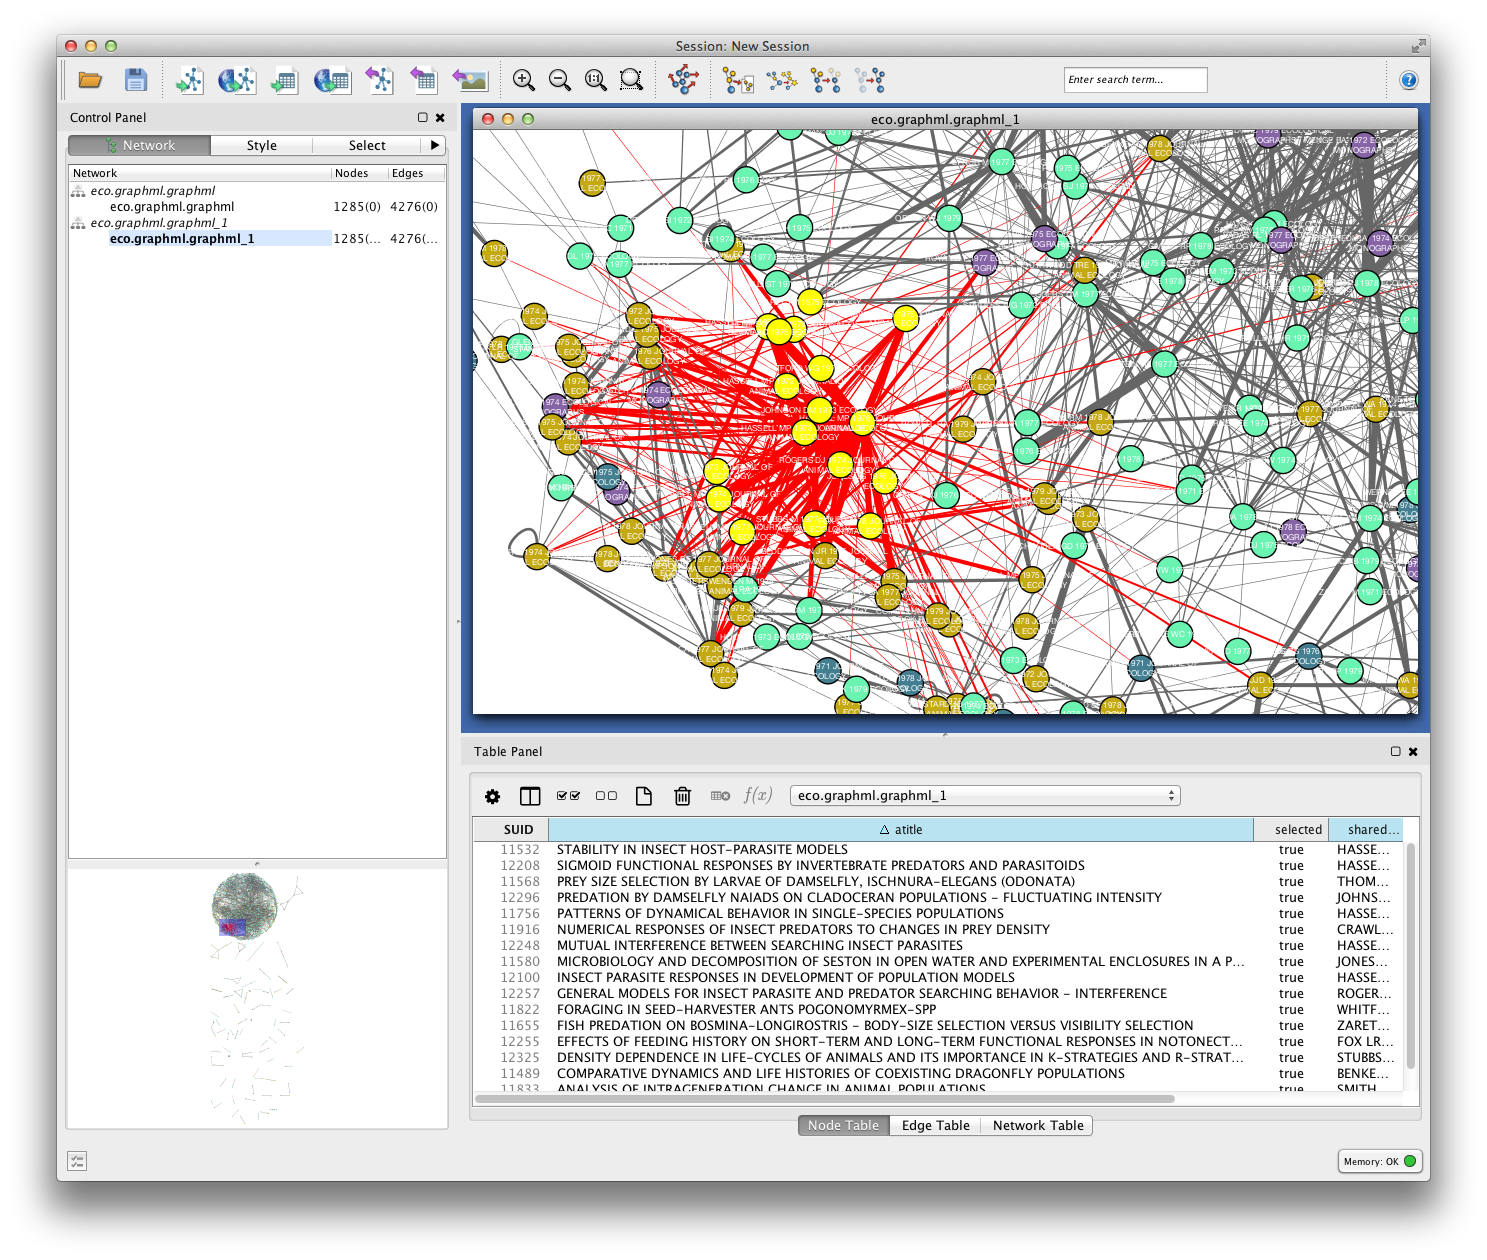
\includegraphics{cyto.4.png}\hfill}


\paragraph{Cluster Detection}
\label{tutorial.bibliocoupling:clusters}\label{tutorial.bibliocoupling:cluster-detection}
Especially if your network is very dense, it may be difficult to find salient clusters
by visual inspection alone. Clustering algorithms provide a useful way to find
groups of nodes that hang together in some way. Most clustering algorithms use an
optimization function to find groups of nodes that are more densely connected among
themselves than with the rest of the network.

One such clustering algorithm in Cytoscape is provided by the MCODE app. To install
the MCODE app:
\begin{enumerate}
\item {} 
Select \code{Apps \textgreater{} App Manager} from the main menu.

\item {} 
Click on the \code{Install Apps} tab, and find MCODE in the list of available apps.

\item {} 
Click the \code{Install} button.

\end{enumerate}

{\hfill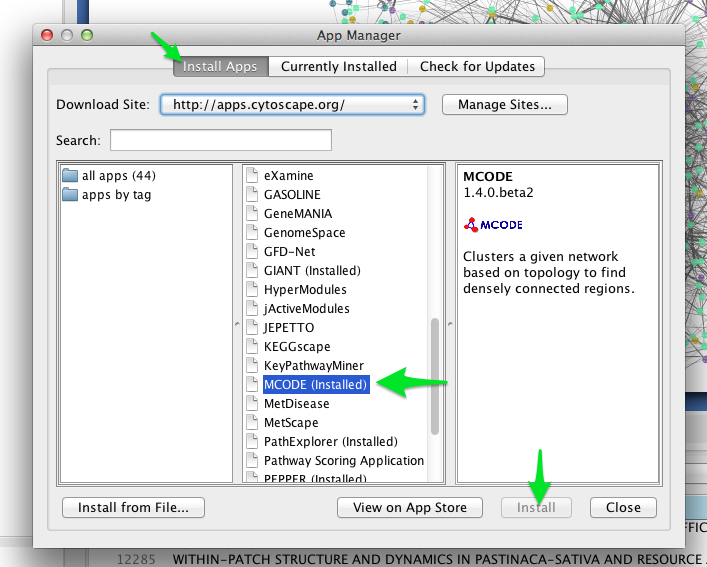
\includegraphics{cyto.5.png}\hfill}

MCODE should now appear in the \code{Apps} menu.

{\hfill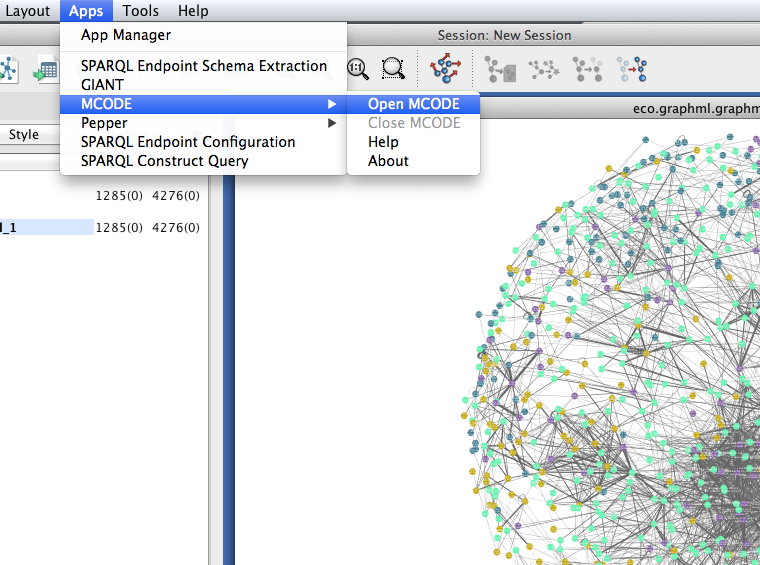
\includegraphics{cyto.6.png}\hfill}
\begin{enumerate}
\item {} 
Select \code{Apps \textgreater{} MCODE \textgreater{} Open MCODE}. A new tab should appear in the \code{Control Panel}
at left.

\item {} 
To adjust the parameters of the MCODE cluster-finding algorithm, expand the
\code{Advanced Options}. MCODE works reasonable well with the default settings.

\item {} 
Click the \code{Analyze current network} button.

\end{enumerate}

{\hfill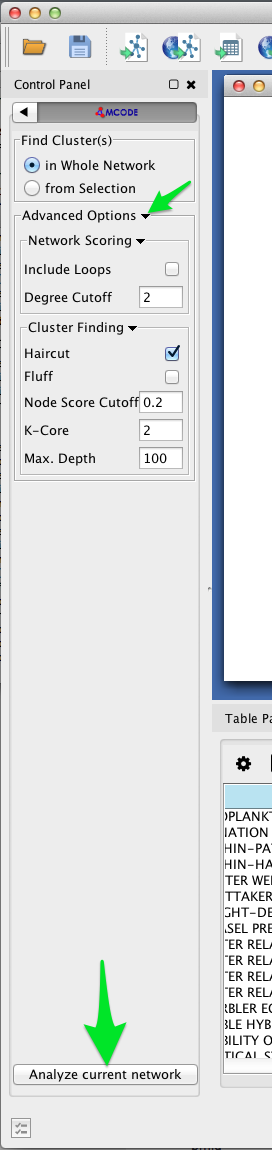
\includegraphics{cyto.7.png}\hfill}

After a few moments, a new window should appear on the right side of the Cytoscape
workspace. Click on a cluster in the \code{Cluster Browser} to select all of the nodes in
that cluster. In some cases, MCODE will find clusters that are not at all obvious
visually. This should give you an impression of the limitations of two-dimensional
layouts for studying network structure, especially in very large, dense networks.

In the example below, MCODE has found a cluster of papers dealing with invertebrate
predators in marine inter-tidal zones.

{\hfill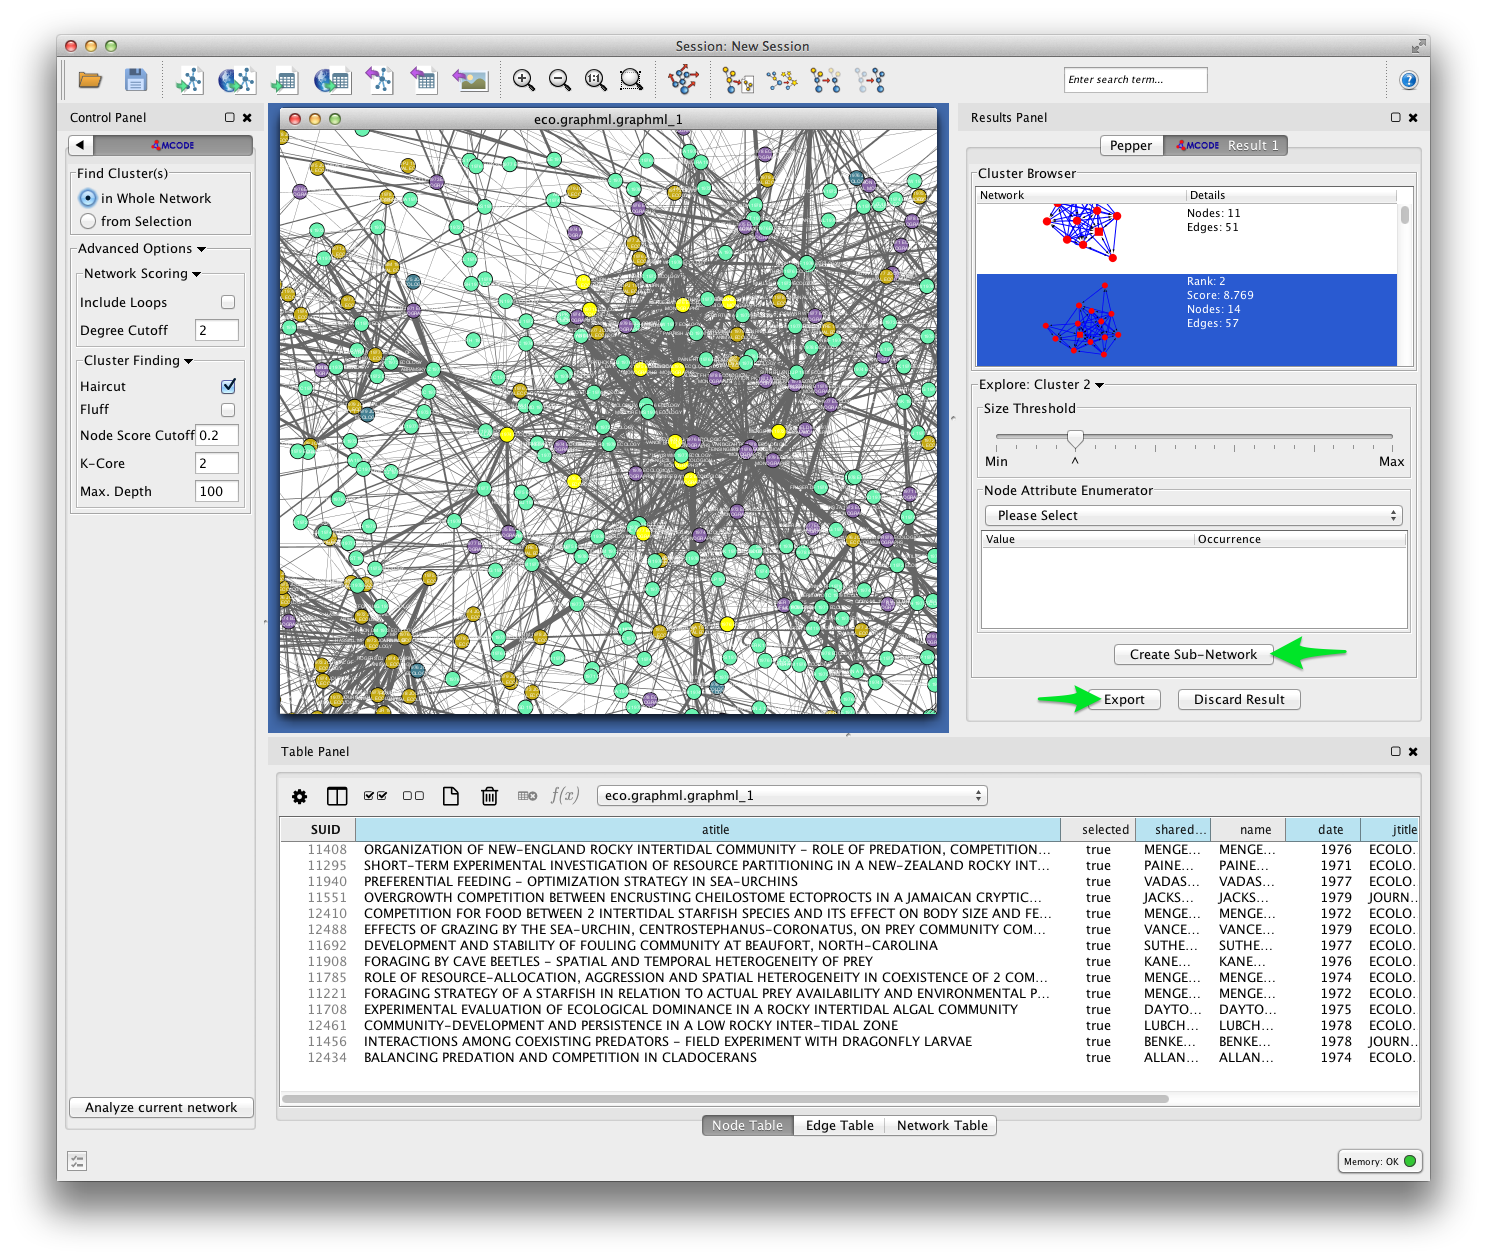
\includegraphics{cyto.8.png}\hfill}

MCODE allows you to create a subnetwork from the selected cluster, or export your results.
Exporting your results produces a table like the one shown below, listing each of the
detected clusters and the papers the belong to them.

\emph{Future versions of Tethne will use this result to generate labels for each cluster based
on the terms that uniquely characterize those groups of papers.}

{\hfill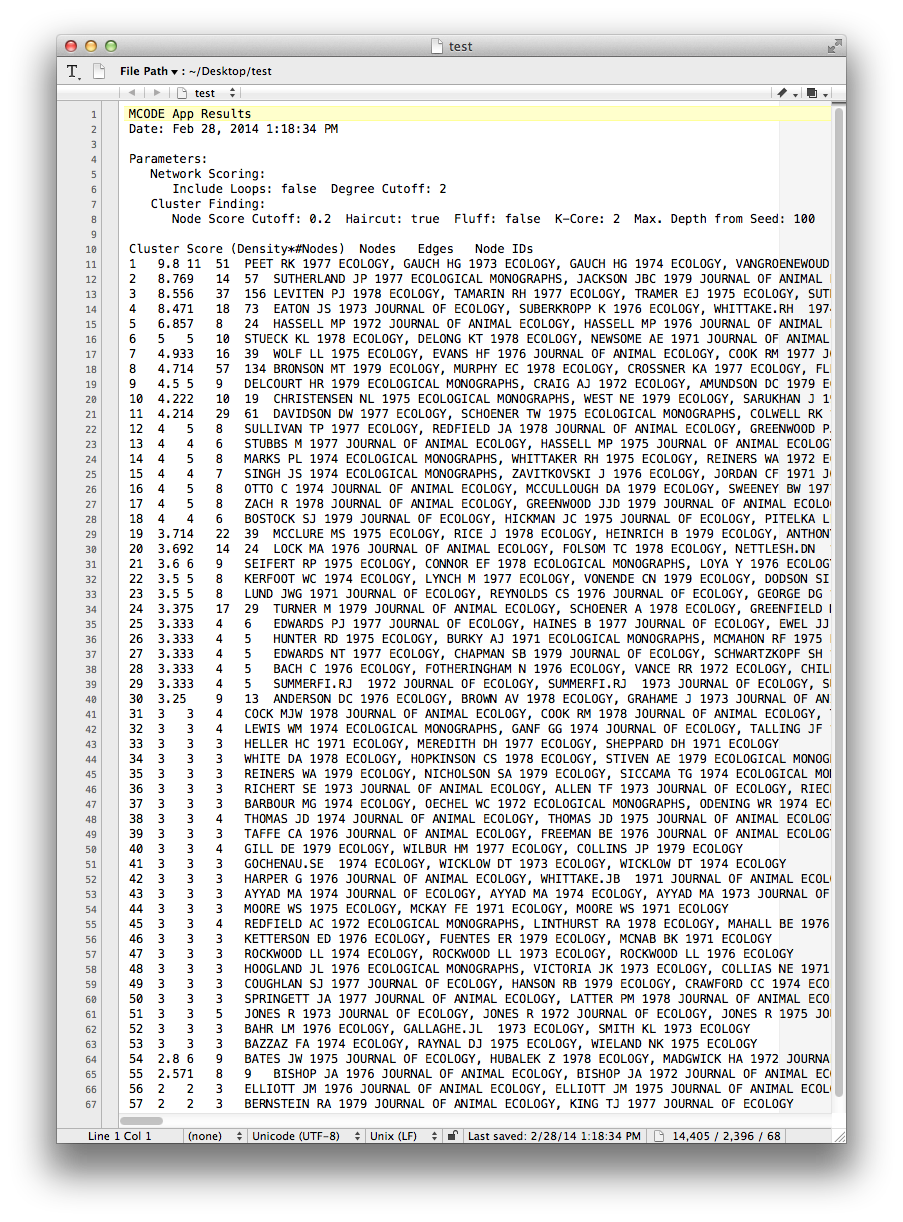
\includegraphics{cyto.9.png}\hfill}

MCODE sets three node attributes:
\begin{itemize}
\item {} 
\code{MCODE\_Cluster} contains the name of the cluster to which each node belongs.

\item {} 
\code{MCODE\_Score} indicates how strongly the neighbors around a node cluster together.
This is similar to the \href{http://en.wikipedia.org/wiki/Clustering\_coefficient\#Local\_clustering\_coefficient}{Local clustering coefficient}

\item {} 
\code{MCODE\_Node\_Status} indicates whether a node is clustered, unclustered, or a seed
node. Seed nodes are the reference nodes chosen by MCODE at the start of the
cluster-detection process.

\end{itemize}

In the visualization below, node fill color is mapped to \code{MCODE\_Cluster}. Node size is
mapped to \code{MCODE\_Node\_Status}: unclustered nodes are small, seed nodes are large, and
clustered nodes are intermediate in size.

{\hfill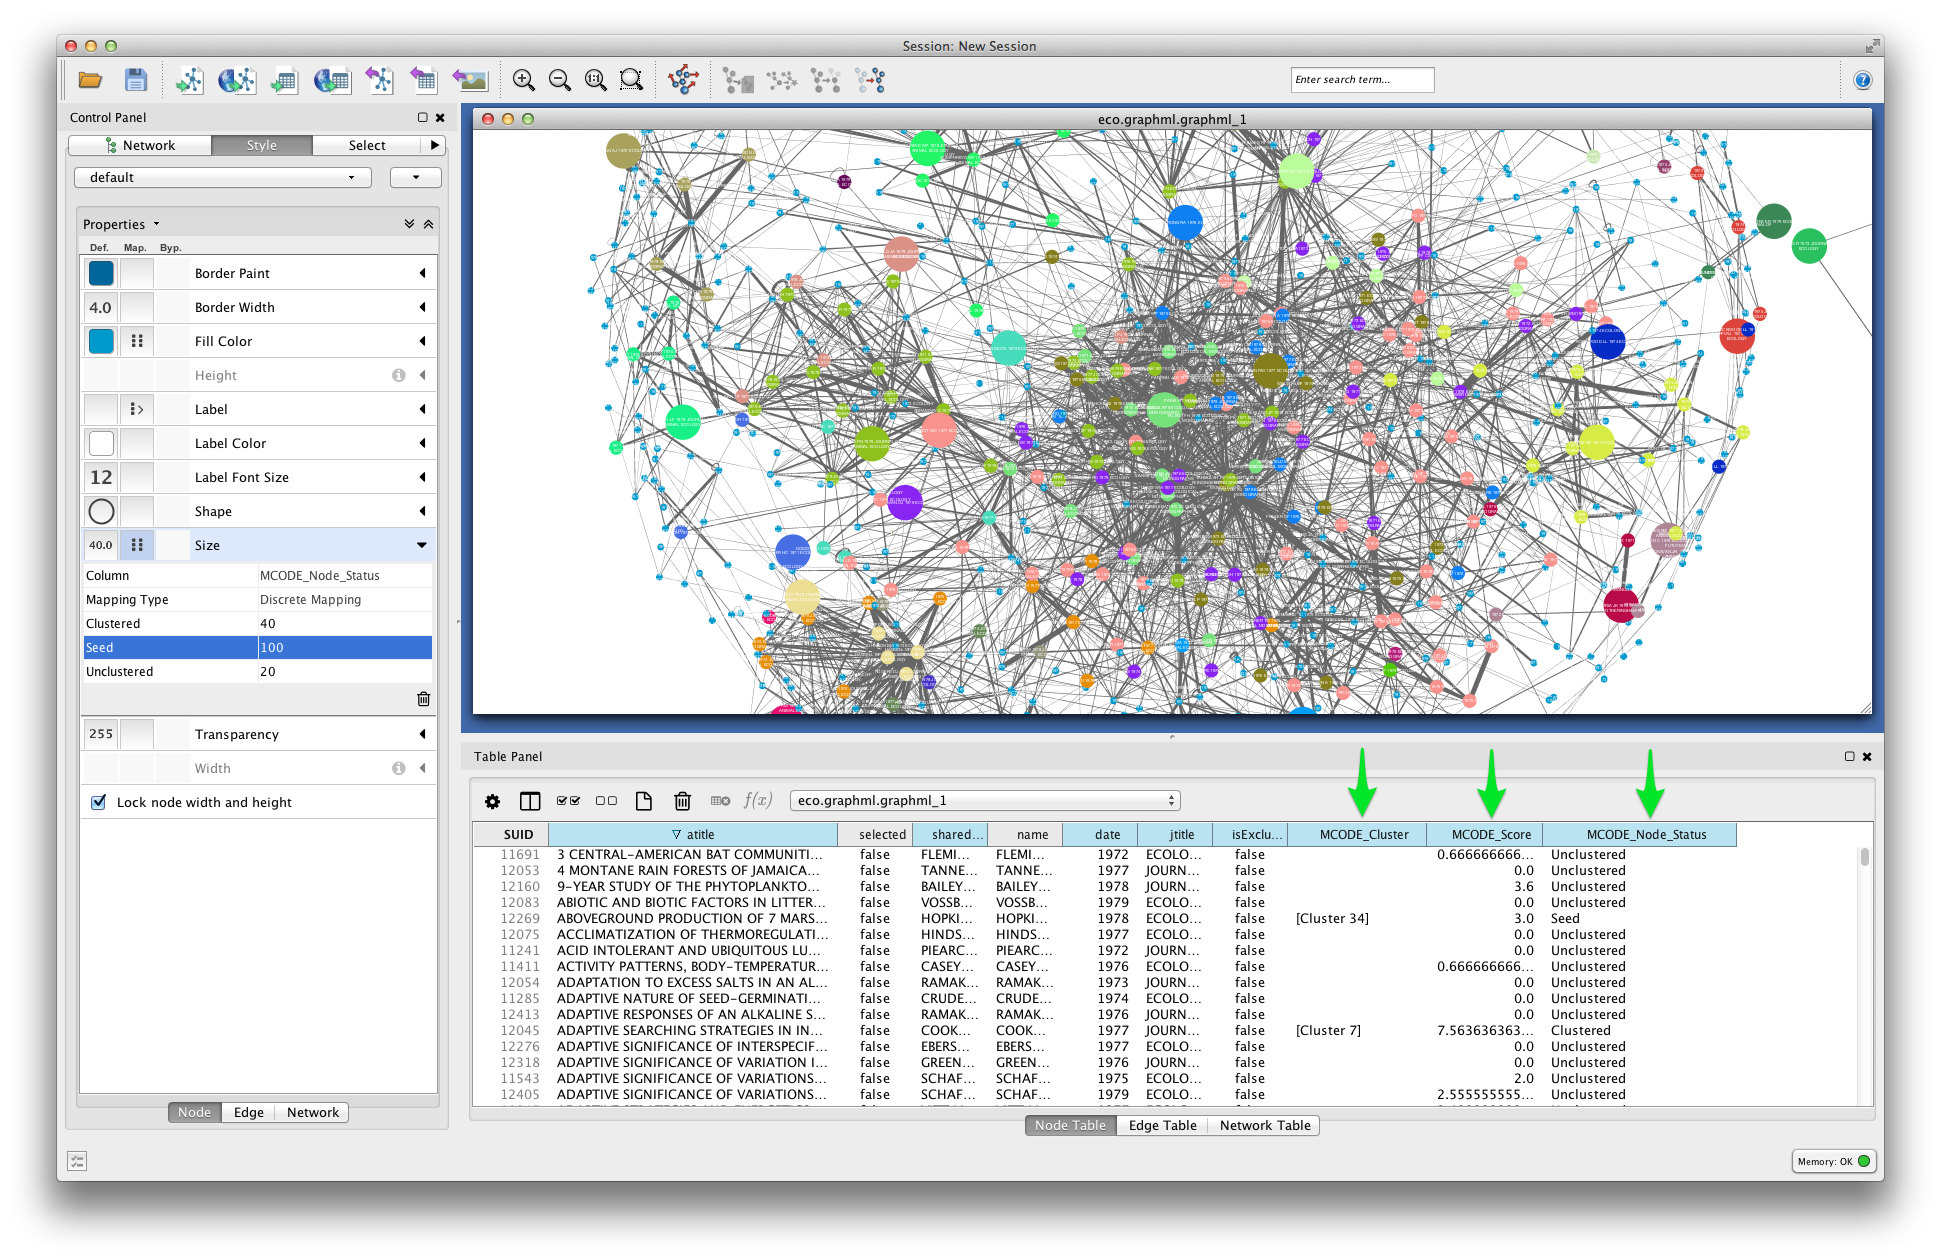
\includegraphics{cyto.10.png}\hfill}


\subsubsection{Evolving Networks}
\label{tutorial.bibliocoupling:evolving-networks}
If your dataset contains records from across a broad time-domain, you may also wish to
view the evolution of your bibliographic coupling network over time. We can do this
by ``slicing'' our {\hyperref[tethne.classes.corpus:tethne.classes.corpus.Corpus]{\code{Corpus}}}, and generating a {\hyperref[tethne.classes.graphcollection:tethne.classes.graphcollection.GraphCollection]{\code{GraphCollection}}} that holds
a set of sequential graphs.


\paragraph{Slicing a Corpus}
\label{tutorial.bibliocoupling:slicing-a-corpus}\label{tutorial.bibliocoupling:id2}
Think of slicing as indexing: we will divide the {\hyperref[tethne.classes.paper:tethne.classes.paper.Paper]{\code{Paper}}}s in our {\hyperref[tethne.classes.corpus:tethne.classes.corpus.Corpus]{\code{Corpus}}}
into bins by publication date, so that later on we can retrieve sets of papers
corresponding to particular time-periods. You can slice your data using the
\code{Corpus.slice()} method.

In this tutorial, we'll slice our {\hyperref[tethne.classes.corpus:tethne.classes.corpus.Corpus]{\code{Corpus}}} using a ``sliding time-window''. Rather
than dividing papers into sequential non-overlapping time periods, the ``time window''
method generates overlapping subsets. For details, see \code{Corpus.slice()}.
\begin{figure}[htbp]
\centering
\capstart

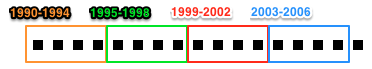
\includegraphics{timeline.timeslice.png}
\caption{\textbf{Time-period} slicing, with a window-size of 4 years.}\end{figure}
\begin{figure}[htbp]
\centering
\capstart

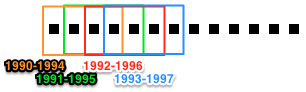
\includegraphics{timeline.timewindow.png}
\caption{\textbf{Time-window} slicing, with a window-size of 4 years and a step-size of 1 year.}\end{figure}

To slice our {\hyperref[tethne.classes.corpus:tethne.classes.corpus.Corpus]{\code{Corpus}}}, we'll use a four-year sliding time-window.

\begin{Verbatim}[commandchars=\\\{\}]
\PYG{g+gp}{\PYGZgt{}\PYGZgt{}\PYGZgt{} }\PYG{n}{MyCorpus}\PYG{p}{(}\PYG{l+s}{\PYGZsq{}}\PYG{l+s}{date}\PYG{l+s}{\PYGZsq{}}\PYG{p}{,} \PYG{l+s}{\PYGZsq{}}\PYG{l+s}{time\PYGZus{}window}\PYG{l+s}{\PYGZsq{}}\PYG{p}{,} \PYG{n}{window\PYGZus{}size}\PYG{o}{=}\PYG{l+m+mi}{4}\PYG{p}{)}
\end{Verbatim}


\paragraph{Building a GraphCollection}
\label{tutorial.bibliocoupling:building-a-graphcollection}
A {\hyperref[tethne.classes.graphcollection:tethne.classes.graphcollection.GraphCollection]{\code{GraphCollection}}} is a set of graphs generated from a {\hyperref[tethne.classes.corpus:tethne.classes.corpus.Corpus]{\code{Corpus}}} or model.
We can generate a GraphCollection (\code{G}) in one step, using the
\code{GraphCollection.build()} method.

A simple example might look like this:

\begin{Verbatim}[commandchars=\\\{\}]
\PYG{g+gp}{\PYGZgt{}\PYGZgt{}\PYGZgt{} }\PYG{n}{G} \PYG{o}{=} \PYG{n}{GraphCollection}\PYG{p}{(}\PYG{p}{)}\PYG{o}{.}\PYG{n}{build}\PYG{p}{(}\PYG{n}{C}\PYG{p}{,} \PYG{l+s}{\PYGZsq{}}\PYG{l+s}{date}\PYG{l+s}{\PYGZsq{}}\PYG{p}{,} \PYG{l+s}{\PYGZsq{}}\PYG{l+s}{papers}\PYG{l+s}{\PYGZsq{}}\PYG{p}{,} \PYG{l+s}{\PYGZsq{}}\PYG{l+s}{bibliographic\PYGZus{}coupling}\PYG{l+s}{\PYGZsq{}}\PYG{p}{)}
\end{Verbatim}

Here we have instructed \code{GraphCollection.build()} to build a graph for each `slice'
along the `date' axis. \code{'papers'} indicates that we want to use a graph method from
the {\hyperref[tethne.networks.papers:module-tethne.networks.papers]{\code{networks.papers}}} submodule, and \code{'bibliographic\_coupling'} indicates the
name of the method from that module that we wish to use.

To apply the parameters from our static network, we can also set the \code{method\_kwargs}
parameter. First we'll define the parameters that we wish to set:

\begin{Verbatim}[commandchars=\\\{\}]
\PYG{g+gp}{\PYGZgt{}\PYGZgt{}\PYGZgt{} }\PYG{n}{method\PYGZus{}kwargs} \PYG{o}{=} \PYG{p}{\PYGZob{}}
\PYG{g+gp}{... }         \PYG{l+s}{\PYGZsq{}}\PYG{l+s}{threshold}\PYG{l+s}{\PYGZsq{}}\PYG{p}{:} \PYG{l+m+mf}{0.05}\PYG{p}{,}
\PYG{g+gp}{... }         \PYG{l+s}{\PYGZsq{}}\PYG{l+s}{node\PYGZus{}attribs}\PYG{l+s}{\PYGZsq{}}\PYG{p}{:} \PYG{p}{[}\PYG{l+s}{\PYGZsq{}}\PYG{l+s}{date}\PYG{l+s}{\PYGZsq{}}\PYG{p}{,} \PYG{l+s}{\PYGZsq{}}\PYG{l+s}{jtitle}\PYG{l+s}{\PYGZsq{}}\PYG{p}{,} \PYG{l+s}{\PYGZsq{}}\PYG{l+s}{atitle}\PYG{l+s}{\PYGZsq{}}\PYG{p}{]}\PYG{p}{,}
\PYG{g+gp}{... }         \PYG{l+s}{\PYGZsq{}}\PYG{l+s}{weighted}\PYG{l+s}{\PYGZsq{}}\PYG{p}{:} \PYG{n+nb+bp}{True}
\PYG{g+gp}{... } \PYG{p}{\PYGZcb{}}
\end{Verbatim}

And then we'll pass those parameters to \code{GraphCollection.build()}.

\begin{Verbatim}[commandchars=\\\{\}]
\PYG{g+gp}{\PYGZgt{}\PYGZgt{}\PYGZgt{} }\PYG{n}{G} \PYG{o}{=} \PYG{n}{GraphCollection}\PYG{p}{(}\PYG{p}{)}\PYG{o}{.}\PYG{n}{build}\PYG{p}{(}\PYG{n}{C}\PYG{p}{,} \PYG{l+s}{\PYGZsq{}}\PYG{l+s}{date}\PYG{l+s}{\PYGZsq{}}\PYG{p}{,} \PYG{l+s}{\PYGZsq{}}\PYG{l+s}{papers}\PYG{l+s}{\PYGZsq{}} \PYG{l+s}{\PYGZsq{}}\PYG{l+s}{bibliographic\PYGZus{}coupling}\PYG{l+s}{\PYGZsq{}}\PYG{p}{,}
\PYG{g+gp}{... }         \PYG{n}{method\PYGZus{}kwargs}\PYG{o}{=}\PYG{n}{method\PYGZus{}kwargs}\PYG{p}{)}
\end{Verbatim}

\code{G} should now contain a series of graphs, one per time-window.

\begin{Verbatim}[commandchars=\\\{\}]
\PYG{g+gp}{\PYGZgt{}\PYGZgt{}\PYGZgt{} }\PYG{n}{G}\PYG{o}{.}\PYG{n}{graphs}
\PYG{g+go}{\PYGZob{}1921: \PYGZlt{}networkx.classes.graph.Graph at 0x10b2692d0\PYGZgt{},}
\PYG{g+go}{     1922: \PYGZlt{}networkx.classes.graph.Graph at 0x10b269c50\PYGZgt{},}
\PYG{g+go}{     1923: \PYGZlt{}networkx.classes.graph.Graph at 0x10b269c10\PYGZgt{},}
\PYG{g+go}{     1924: \PYGZlt{}networkx.classes.graph.Graph at 0x10b2695d0\PYGZgt{},}
\PYG{g+go}{     1925: \PYGZlt{}networkx.classes.graph.Graph at 0x10b269dd0\PYGZgt{},}
\PYG{g+go}{     1926: \PYGZlt{}networkx.classes.graph.Graph at 0x10a88bb90\PYGZgt{},}
\PYG{g+go}{     1927: \PYGZlt{}networkx.classes.graph.Graph at 0x10a88b0d0\PYGZgt{},}
\PYG{g+go}{     1928: \PYGZlt{}networkx.classes.graph.Graph at 0x10b269a50\PYGZgt{},}
\PYG{g+go}{     1929: \PYGZlt{}networkx.classes.graph.Graph at 0x10b269b50\PYGZgt{},}
\PYG{g+go}{     1930: \PYGZlt{}networkx.classes.graph.Graph at 0x10b269790\PYGZgt{},}
\PYG{g+go}{     1931: \PYGZlt{}networkx.classes.graph.Graph at 0x10b269d50\PYGZgt{},}
\PYG{g+go}{     1932: \PYGZlt{}networkx.classes.graph.Graph at 0x10a88bed0\PYGZgt{}\PYGZcb{}}
\end{Verbatim}

Here the date keys (1921-1932) refer to the start-date of each time-window. So the key
1921 refers to the time-window 1921-1924.


\subsubsection{Visualizing a Dynamic Network}
\label{tutorial.bibliocoupling:visualizing-a-dynamic-network}
Use the {\hyperref[tethne.writers.collection:tethne.writers.collection.to_dxgmml]{\code{writers.collection.to\_dxgmml()}}} method to create a \href{https://code.google.com/p/dynnetwork/wiki/DynamicXGMML}{dynamic XGMML} network data file.

\begin{Verbatim}[commandchars=\\\{\}]
\PYG{g+gp}{\PYGZgt{}\PYGZgt{}\PYGZgt{} }\PYG{k+kn}{from} \PYG{n+nn}{tethne.writers} \PYG{k+kn}{import} \PYG{n}{collection}
\PYG{g+gp}{\PYGZgt{}\PYGZgt{}\PYGZgt{} }\PYG{n}{collection}\PYG{o}{.}\PYG{n}{to\PYGZus{}dxgmml}\PYG{p}{(}\PYG{n}{G}\PYG{p}{,} \PYG{l+s}{\PYGZsq{}}\PYG{l+s}{/path/to/my/dynamicnetwork.xgmml}\PYG{l+s}{\PYGZsq{}}\PYG{p}{)}
\end{Verbatim}

In Cytoscape, import your .xgmml file by selecting
\code{File \textgreater{} Import \textgreater{} Dynamic Network \textgreater{} XGMML File...}. Apply a force-directed or
spring-embedded layout.

{\hfill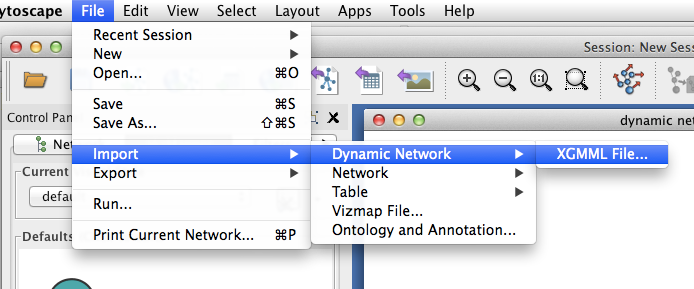
\includegraphics{coauthors.34.png}\hfill}

In the Control Panel, select the \code{Dynamic Network} tab.
\begin{enumerate}
\item {} 
Set the time resolution to roughly match the time-range of your network. In the
example below, the network covers about 35 years, so a resolution of 1/50 was selected.

\item {} 
Set \code{Time smoothness} to \code{0 ms}.

\item {} 
Use the slider to move through the states of your dynamic network. To view all states
in succession, use the \code{\textless{}\textless{} Play} and \code{Play \textgreater{}\textgreater{}} buttons.

\end{enumerate}

{\hfill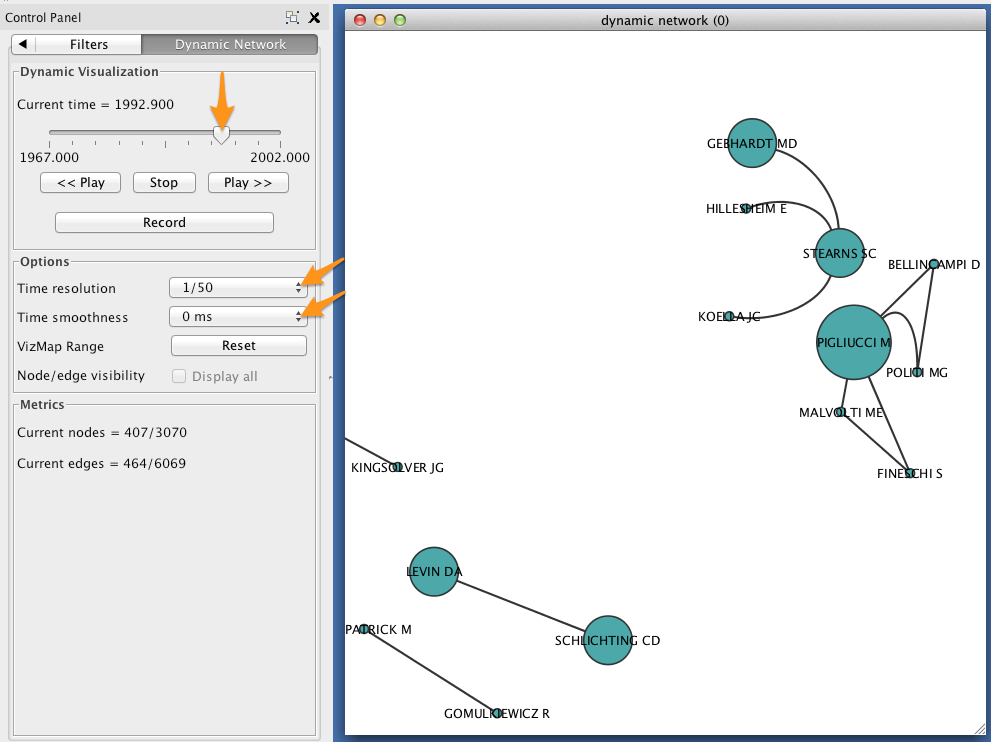
\includegraphics{coauthors.37.png}\hfill}


\subsection{Coauthorship Networks}
\label{tutorial.coauthors:coauthorship}\label{tutorial.coauthors:coauthorship-networks}\label{tutorial.coauthors::doc}\setbox0\vbox{
\begin{minipage}{0.95\linewidth}
\begin{itemize}
\item {} 
{\hyperref[tutorial.coauthors:getting-started]{Getting Started}}

\item {} 
{\hyperref[tutorial.coauthors:reading-wos-data]{Reading WoS Data}}

\item {} 
{\hyperref[tutorial.coauthors:slicing-a-corpus]{Slicing a Corpus}}

\item {} 
{\hyperref[tutorial.coauthors:building-a-static-co-author-graph]{Building a Static Co-author Graph}}

\item {} 
{\hyperref[tutorial.coauthors:visualize-the-static-graph]{Visualize the Static Graph}}
\begin{itemize}
\item {} 
{\hyperref[tutorial.coauthors:write-the-graph-to-graphml]{Write the Graph to GraphML}}

\item {} 
{\hyperref[tutorial.coauthors:cytoscape]{Cytoscape}}

\item {} 
{\hyperref[tutorial.coauthors:inter-institutional-collaboration-in-gephi]{Inter-institutional Collaboration in Gephi}}

\end{itemize}

\item {} 
{\hyperref[tutorial.coauthors:coauthorship-network-evolution]{Coauthorship network evolution}}
\begin{itemize}
\item {} 
{\hyperref[tutorial.coauthors:building-a-graphcollection]{Building a GraphCollection}}

\item {} 
{\hyperref[tutorial.coauthors:attachment-probability]{Attachment Probability}}

\item {} 
{\hyperref[tutorial.coauthors:dynamic-xgmml]{Dynamic XGMML}}

\item {} 
{\hyperref[tutorial.coauthors:id16]{Cytoscape}}

\end{itemize}

\end{itemize}
\end{minipage}}
\begin{center}\setlength{\fboxsep}{5pt}\shadowbox{\box0}\end{center}

\begin{notice}{note}{Note:}
This tutorial was developed for the course \href{http://devo-evo.lab.asu.edu/methods}{Introduction to Digital \&
Computational Methods in the Humanities (HPS)},
created and taught by \href{http://devo-evo.lab.asu.edu/?q=damerow}{Julia Damerow} and
\href{http://gradinfo.cbs.asu.edu/?page\_id=49}{Erick Peirson}.
\end{notice}

Coauthorship networks are among the most popular models for studying the structure of
research communities, due in no small part to the ease with which coauthorship networks
can be generated.


\subsubsection{Getting Started}
\label{tutorial.coauthors:getting-started}
Before you begin, be sure to install the latest version of Tethne. Consult the
\emph{installation} guide for details.

\textbf{If you run into problems}, don't panic. Tethne is under active development, and there
are certainly bugs to be found. Please report any problems, including errors in this
tutorial, via our \href{https://github.com/diging/tethne/issues?state=open}{GitHub issue tracker}.

For this tutorial, you'll need some citation data from the ISI Web of Science. If this is
your first time working with WoS citation data, check out {\hyperref[tutorial.getting_data:gettingdata]{\emph{Getting Bibliographic Data}}}. We'll
assume that you have downloaded a few sets of records from WoS, and stored them all in
the same directory.

\begin{Verbatim}[commandchars=\\\{\}]
\PYG{g+gp}{\PYGZgt{}\PYGZgt{}\PYGZgt{} }\PYG{n}{datapath} \PYG{o}{=} \PYG{l+s}{\PYGZsq{}}\PYG{l+s}{/path/to/my/data/directory}\PYG{l+s}{\PYGZsq{}}
\end{Verbatim}


\subsubsection{Reading WoS Data}
\label{tutorial.coauthors:reading-wos-data}
You can parse WoS data from one or multiple field-tagged data files, using the methods
in the {\hyperref[tethne.readers:module-tethne.readers]{\code{readers}}} module. Since we're working with multiple data files, we'll
use the \code{readers.wos.corpus\_from\_dir} method to parse the WoS data and create
a new {\hyperref[tethne.classes.corpus:tethne.classes.corpus.Corpus]{\code{Corpus}}} called \code{MyCorpus}.

\begin{Verbatim}[commandchars=\\\{\}]
\PYG{g+gp}{\PYGZgt{}\PYGZgt{}\PYGZgt{} }\PYG{k+kn}{from} \PYG{n+nn}{tethne.readers} \PYG{k+kn}{import} \PYG{n}{wos}
\PYG{g+gp}{\PYGZgt{}\PYGZgt{}\PYGZgt{} }\PYG{n}{MyCorpus} \PYG{o}{=} \PYG{n}{wos}\PYG{o}{.}\PYG{n}{corpus\PYGZus{}from\PYGZus{}dir}\PYG{p}{(}\PYG{n}{datapath}\PYG{p}{)}
\end{Verbatim}


\subsubsection{Slicing a Corpus}
\label{tutorial.coauthors:slicing-a-corpus}
In this tutorial, we will analyze the evolution of a coauthorship network over time. To do
this, we will slice our data using the \code{date} field of each paper in our dataset.

Think of slicing as indexing: we will divide the {\hyperref[tethne.classes.paper:tethne.classes.paper.Paper]{\code{Paper}}}s in our {\hyperref[tethne.classes.corpus:tethne.classes.corpus.Corpus]{\code{Corpus}}}
into bins by publication date, so that later on we can retrieve sets of papers
corresponding to particular time-periods. You can slice your data using the
\code{Corpus.slice()} method.

We'll use the \code{time\_period} slice method, which means that the data will be divided into
subsets each containing data from a particular time period. The default window size is 1,
and the window will advance by 1 year in each slice.

We will assume that the first coauthorship event represents (with some delay) the
commencement of a collaborative relationship between two researchers, and that this
social tie does not simply disappear after the coauthorship event. A more sophisticated
model might parameterize the decay of potential social influence after a coauthorship
event, but for the purpose of this tutorial we will assume that those social ties are
effectively permanent. In order to realize this assumption in the final coauthorship
model, we will  use the cumulative slicing option, which means that the data from each
time period will contain data from all of the previous time-periods. In other words, the
1957 subset will contain data from 1957, and the 1958 subset will contain data from 1957
and 1958. This means that coauthorship ties will be added in each sequential graph, but
never removed.

Use the \code{tethne.data.DataCollection.slice()} method to slice your data.

\begin{Verbatim}[commandchars=\\\{\}]
\PYG{g+gp}{\PYGZgt{}\PYGZgt{}\PYGZgt{} }\PYG{n}{MyCorpus}\PYG{o}{.}\PYG{n}{slice}\PYG{p}{(}\PYG{l+s}{\PYGZsq{}}\PYG{l+s}{date}\PYG{l+s}{\PYGZsq{}}\PYG{p}{,} \PYG{l+s}{\PYGZsq{}}\PYG{l+s}{time\PYGZus{}period}\PYG{l+s}{\PYGZsq{}}\PYG{p}{,} \PYG{n}{window\PYGZus{}size}\PYG{o}{=}\PYG{l+m+mi}{1}\PYG{p}{,} \PYG{n}{cumulative}\PYG{o}{=}\PYG{n+nb+bp}{True}\PYG{p}{)}
\end{Verbatim}


\subsubsection{Building a Static Co-author Graph}
\label{tutorial.coauthors:building-a-static-co-author-graph}
Tethne will generate a graph using the \code{AU} field in your WoS data. See
{\hyperref[tutorial.getting_data:fieldtagged]{\emph{Structure of the WoS Field-Tagged Data File}}} for more information about the fields available in a WoS datafile.

To get a sense of the overall structure of the graph, we can first build a static
coauthorship graph by calling the {\hyperref[tethne.networks.authors:tethne.networks.authors.coauthors]{\code{networks.authors.coauthors()}}} method directly.

\begin{Verbatim}[commandchars=\\\{\}]
\PYG{g+gp}{\PYGZgt{}\PYGZgt{}\PYGZgt{} }\PYG{k+kn}{from} \PYG{n+nn}{tethne.networks} \PYG{k+kn}{import} \PYG{n}{authors}
\PYG{g+gp}{\PYGZgt{}\PYGZgt{}\PYGZgt{} }\PYG{n}{ca\PYGZus{}graph} \PYG{o}{=} \PYG{n}{authors}\PYG{o}{.}\PYG{n}{coauthors}\PYG{p}{(}\PYG{n}{MyCorpus}\PYG{o}{.}\PYG{n}{all\PYGZus{}papers}\PYG{p}{(}\PYG{p}{)}\PYG{p}{)}
\end{Verbatim}


\subsubsection{Visualize the Static Graph}
\label{tutorial.coauthors:coauthors-to-graphml}\label{tutorial.coauthors:visualize-the-static-graph}

\paragraph{Write the Graph to GraphML}
\label{tutorial.coauthors:write-the-graph-to-graphml}
\href{http://graphml.graphdrawing.org}{GraphML} is a widely-used static network data format.
We will write our graph to GraphML for visualization in Cytoscape.

Use the {\hyperref[tethne.writers.graph:tethne.writers.graph.to_graphml]{\code{to\_graphml()}}} method in {\hyperref[tethne.writers.collection:module-tethne.writers.collection]{\code{writers.collection}}} to create a GraphML
data file.

\begin{Verbatim}[commandchars=\\\{\}]
\PYG{g+gp}{\PYGZgt{}\PYGZgt{}\PYGZgt{} }\PYG{k+kn}{from} \PYG{n+nn}{tethne.writers} \PYG{k+kn}{import} \PYG{n}{graph}
\PYG{g+gp}{\PYGZgt{}\PYGZgt{}\PYGZgt{} }\PYG{n}{graph}\PYG{o}{.}\PYG{n}{to\PYGZus{}graphml}\PYG{p}{(}\PYG{n}{ca\PYGZus{}graph}\PYG{p}{,} \PYG{l+s}{\PYGZsq{}}\PYG{l+s}{/path/to/my/graphmlfile.grapml}\PYG{l+s}{\PYGZsq{}}\PYG{p}{)}
\end{Verbatim}


\paragraph{Cytoscape}
\label{tutorial.coauthors:cytoscape}
Cytoscape was developed in 2002, with funding from the National Instute of General Medical
Sciences and the National Resource for Network Biology. The primary user base is the
biomedical research community, especially systems biologists who study gene or protein
interaction networks and pathways.

You can download Cytoscape 3 from url\{\href{http://www.cytoscape.org}{http://www.cytoscape.org}\}. This tutorial assumes
that you are using Cytoscape 3.0.2.


\subparagraph{Import}
\label{tutorial.coauthors:import}
In Cytoscape, import your network by selecting \code{File \textgreater{} Import \textgreater{} Network \textgreater{} From file...}
and selecting the GraphML file generated by Tethne in your output directory.

Apply a Force Directed layout by selecting \code{Layout \textgreater{} Prefuse Force Directed Layout}.

Coauthorship networks are usually comprised of a very large connected component, and many
very small components. For convenience, we will only look at the few largest components.
Select the largest connected components (click and drag to create a selection box). Then
create a new network with those selected components: select
\code{File \textgreater{} New \textgreater{} Networks \textgreater{} From selected nodes, all edges}.

{\hfill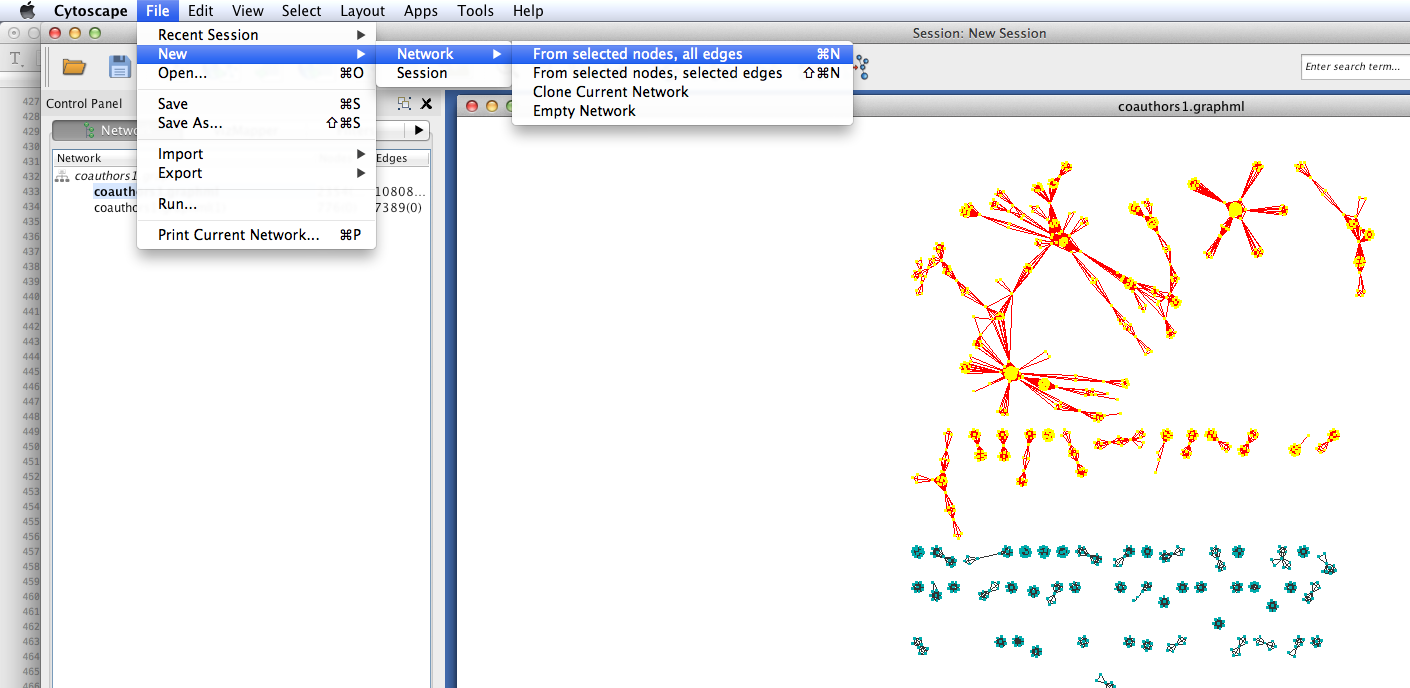
\includegraphics{coauthors.7.png}\hfill}

You should now see a new graph in its own viewing window, containing only the components
that you selected.

{\hfill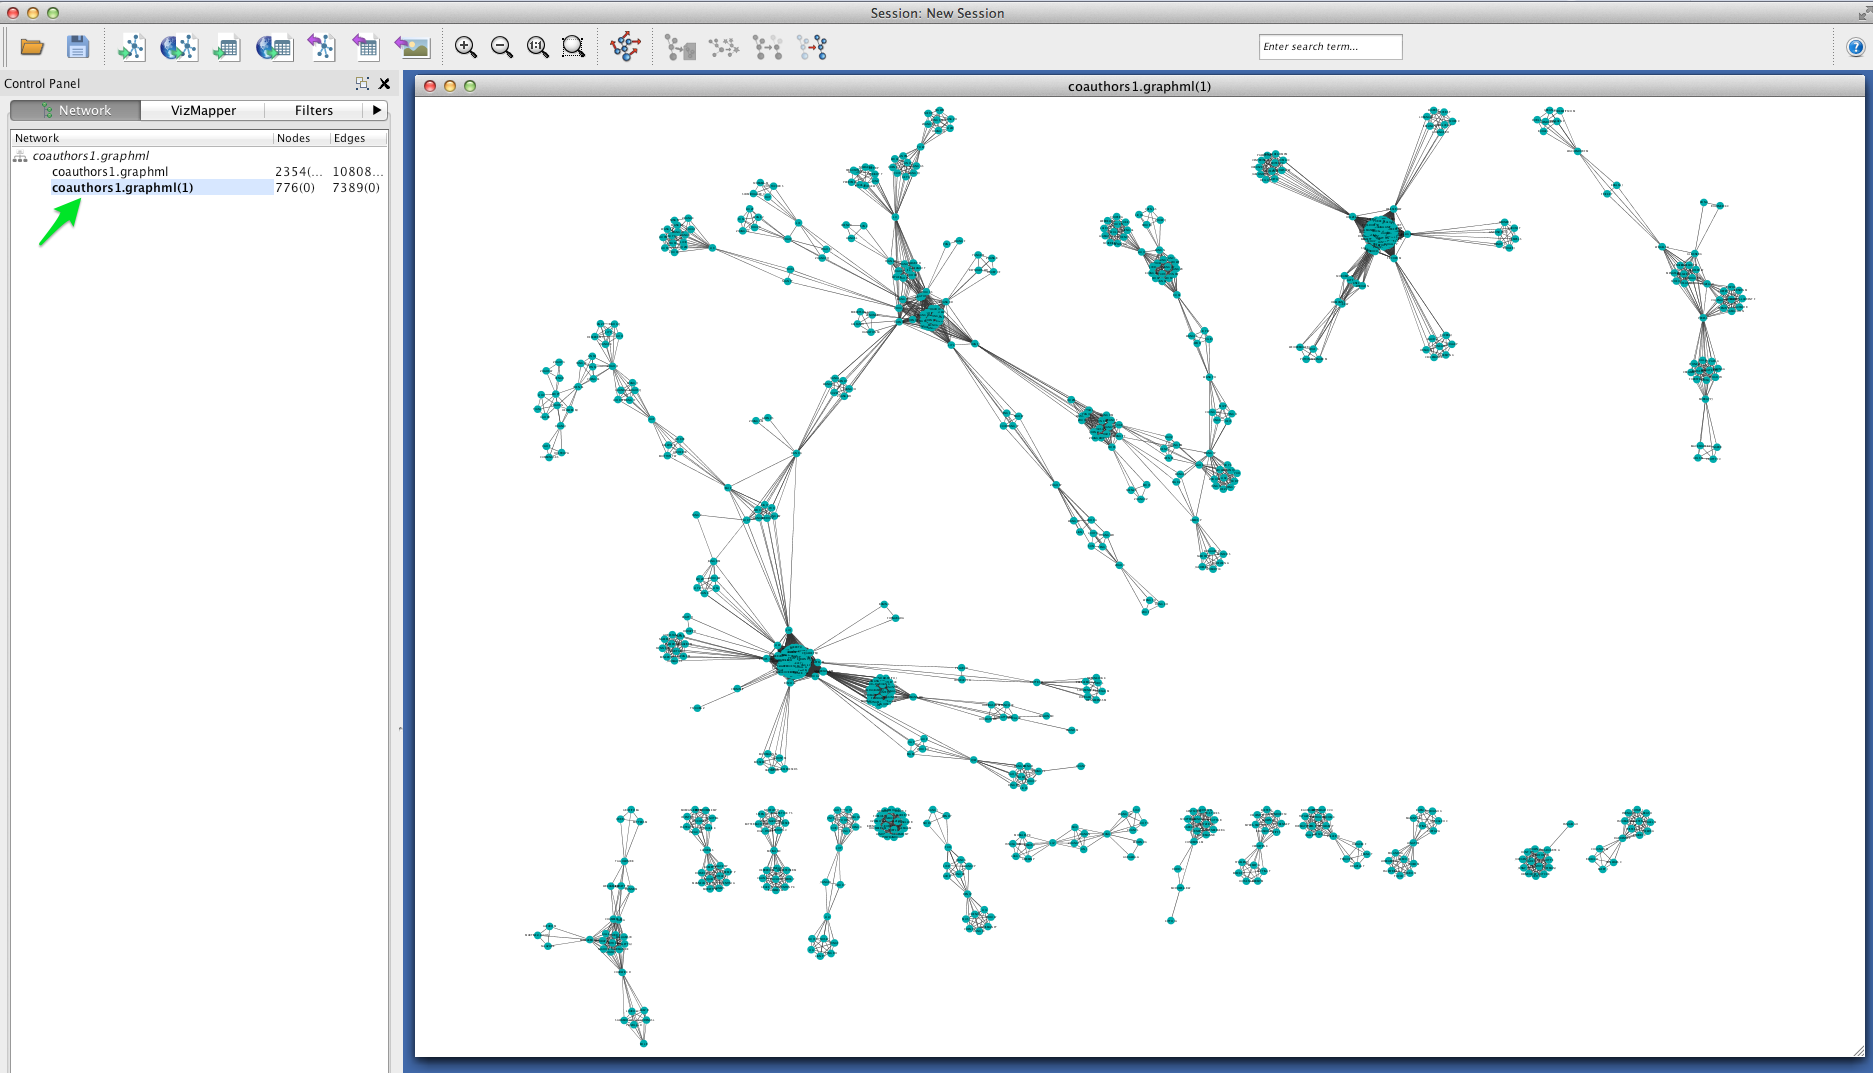
\includegraphics{coauthors.8.png}\hfill}


\subparagraph{Betweenness Centrality}
\label{tutorial.coauthors:betweenness-centrality}
This coauthorship network is clearly very modular: there are dense clusters connected by a
few linking nodes that occupy sparse areas of the graph (so-called ``structural holes''). We
can identify the structurally most-significant actors by their ``betweenness centrality.''
Formally, betweenness centrality is a measure of the number of shortest paths that pass
through a particular node.

Run Cytoscape's network-analysis algorithm. Go to
\code{Tools \textgreater{} NetworkAnalyzer \textgreater{} Network Analysis \textgreater{} Analyze Network}.

{\hfill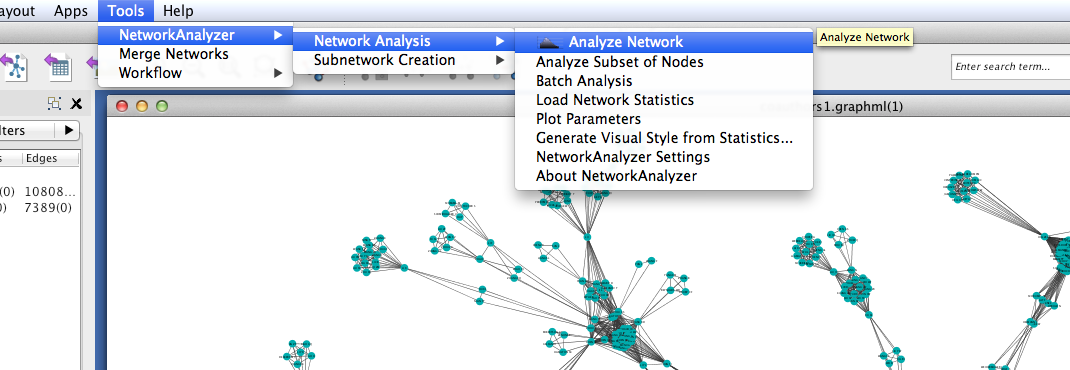
\includegraphics{coauthors.9.png}\hfill}

Cytoscape may ask you whether to interpret the network as directed or undirected. A
coauthorship network is always undirected, since coauthorship is a symmetric relationship.

{\hfill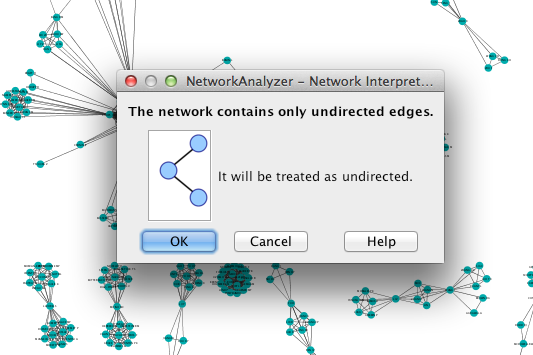
\includegraphics{coauthors.10.png}\hfill}

Once network analysis is complete, a window titled \code{Results Panel} will appear. Close
this window.

{\hfill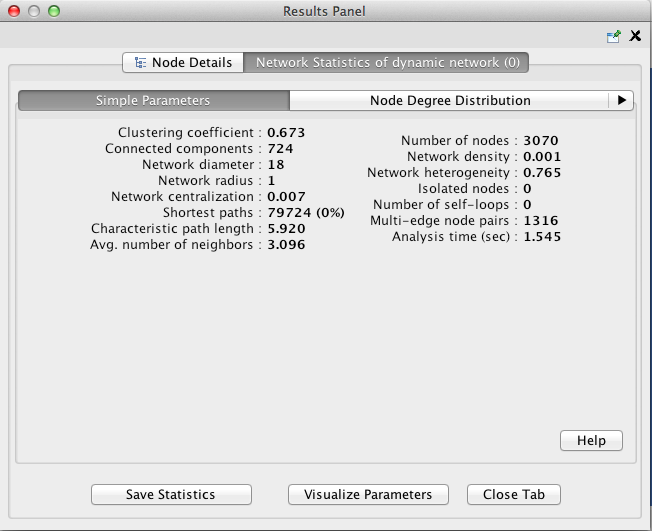
\includegraphics{coauthors.11.png}\hfill}

To visualize the betweenness centrality of each node, create a new visual mapping.
\begin{enumerate}
\item {} 
Go to the VizMapper tab, in the left part of the Cytoscape workspace.

\item {} 
Find \code{Node Size} in the unused visual properties, and double-click to move it to the
\code{Node Visual Properties} list.

\item {} 
Click in the area to the right of \code{Node Size} and select \code{BetweennessCentrality}.

\item {} 
Click in the area to the right of \code{Mapping Type} and select \code{Continuous Mapping}.

\end{enumerate}

{\hfill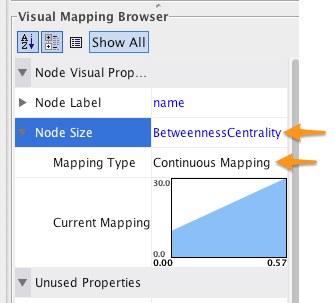
\includegraphics{coauthors.12.png}\hfill}

To change the size - centrality mapping function, double-click on the figure to the right
of \code{Curent Mapping}, and drag the red open boxes up and down to change the angle of the
function.

{\hfill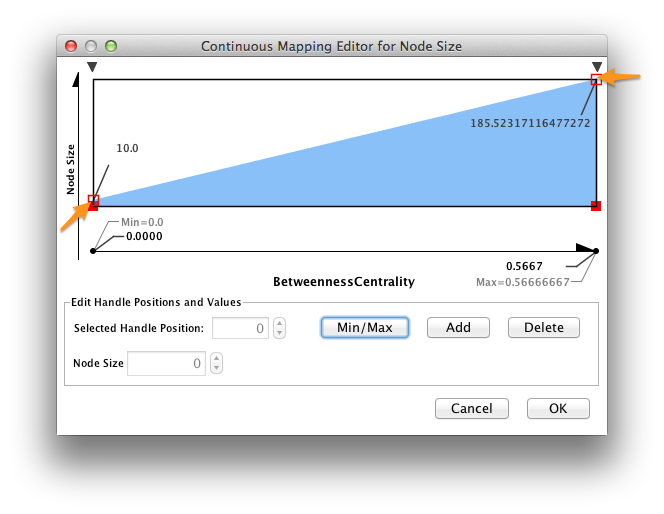
\includegraphics{coauthors.13.png}\hfill}

The largest nodes are the most central nodes in their respective connected components.
These are the nodes most responsible for connecting disparate clusters in the network.

To see a list of the most central nodes, set the Table Panel to show all nodes.

{\hfill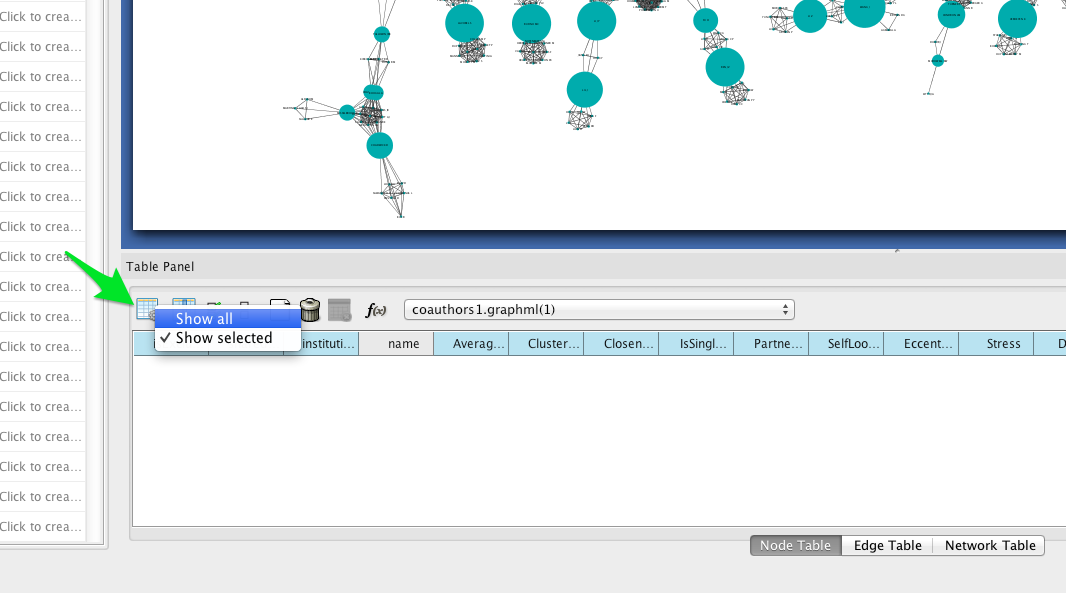
\includegraphics{coauthors.14.png}\hfill}

Then sort by betweenness centrality by clicking on the column header in the Node Table
(you may have to click twice to sort in descending order).

{\hfill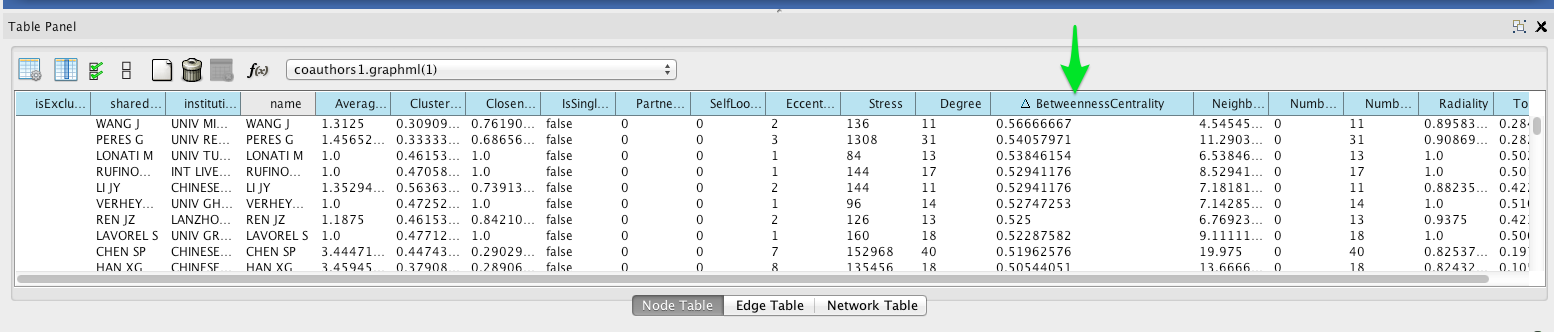
\includegraphics{coauthors.15.png}\hfill}


\subparagraph{Institutional affiliation}
\label{tutorial.coauthors:institutional-affiliation}
Wherever possible, Tethne includes institutional affiliations for authors as node
attributes. You should see institutions listed in the Node Table.

{\hfill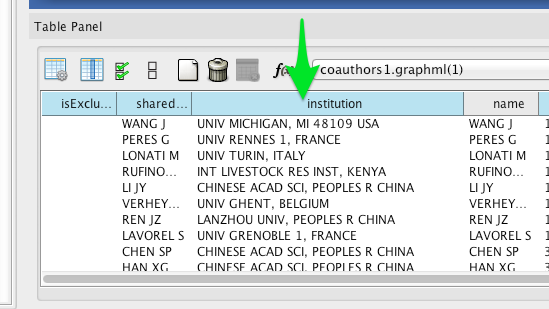
\includegraphics{coauthors.16.png}\hfill}

Create a visual mapping for institutional affiliation.
\begin{enumerate}
\item {} 
Go to the VizMapper.

\item {} 
Find \code{Node Fill Color} in the unused visual properties, and double-click to activate.

\item {} 
Click to the right of {\color{red}\bfseries{}{}`{}`}Node Fill Color'' and select {\color{red}\bfseries{}{}`{}`}institution'`.

\item {} 
Set the {\color{red}\bfseries{}{}`{}`}Mapping Type'' to {\color{red}\bfseries{}{}`{}`}Discrete Mapping.'' A list of institutions should appear
below {\color{red}\bfseries{}{}`{}`}Mapping Type.'`

\item {} 
Right-click on \code{Discrete Mapping'{'}, and select
{}`{}`Mapping Value Generators \textgreater{} Random Color}.

\end{enumerate}

{\hfill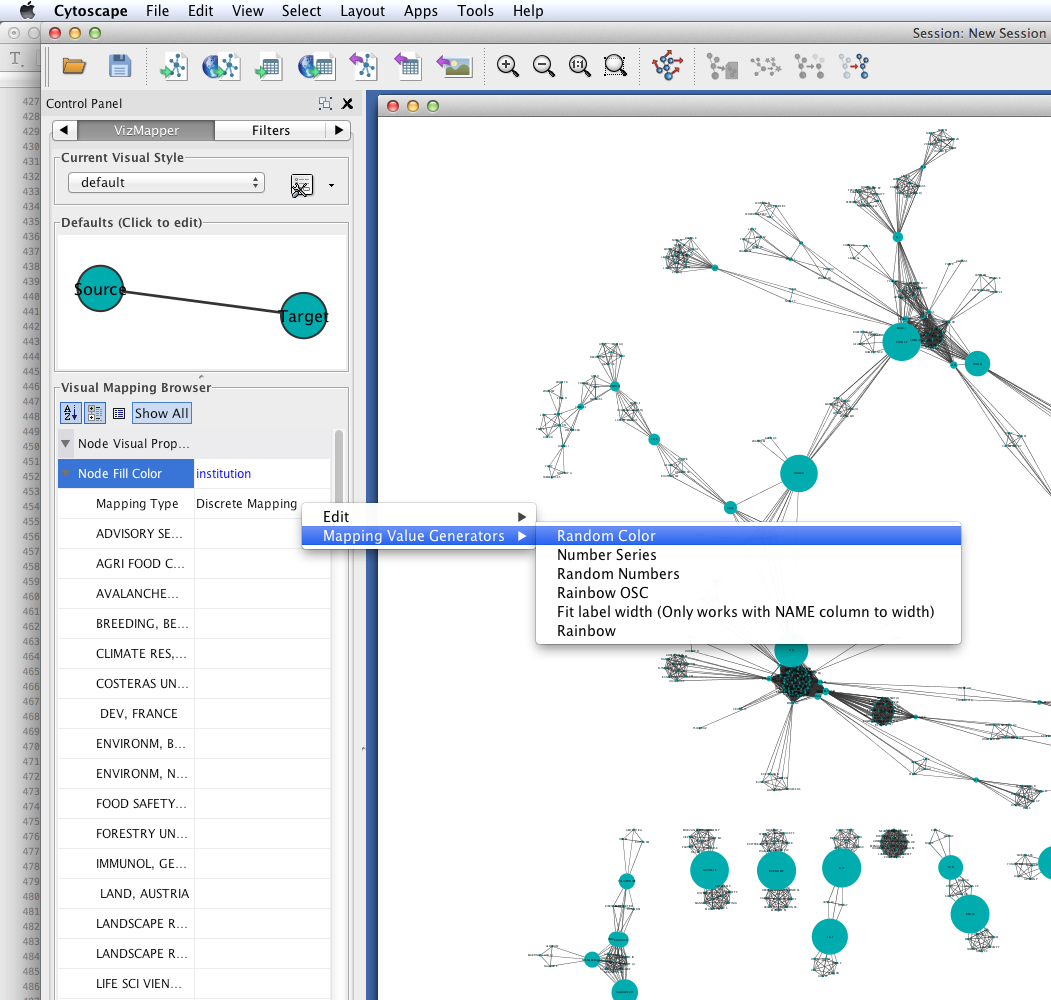
\includegraphics{coauthors.17.png}\hfill}

Each node should now be colored according to its institutional affiliation.
Inspecting the network yields an immediate impression of whether coauthorship clusters are
due to affiliation with the same institution.

{\hfill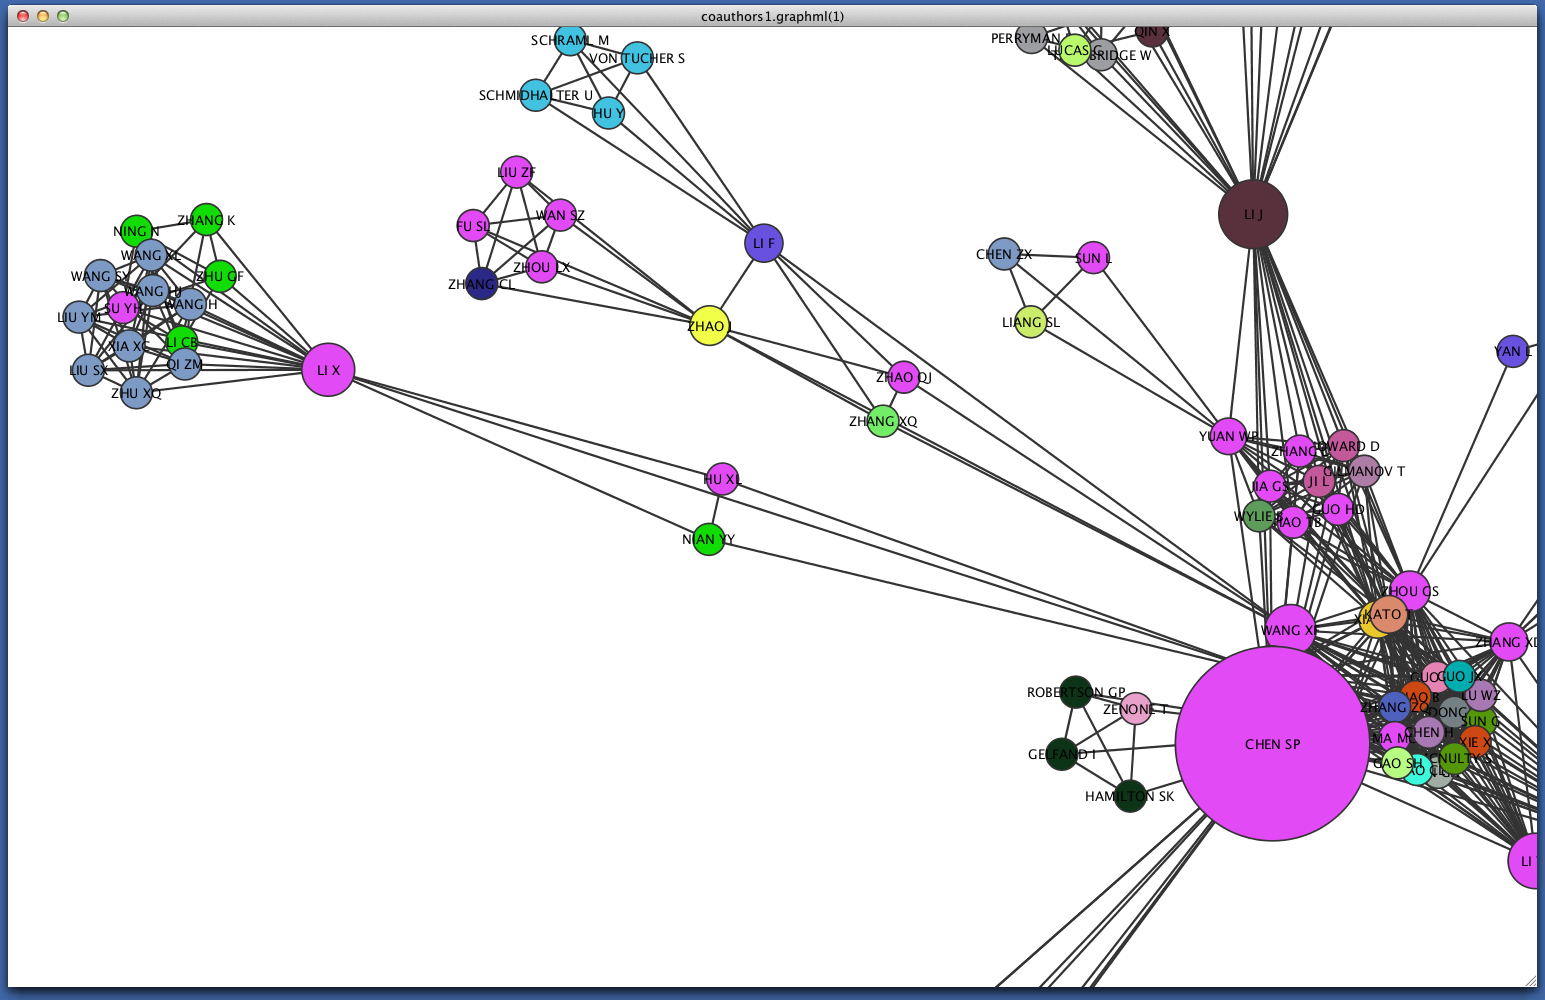
\includegraphics{coauthors.18.png}\hfill}

Since some institutions may be colored quite similarly, select a cluster to view the
specific institutional affiliation of each node. You may need to set the Node Table to
\code{show selected} rather than \code{show all}.

{\hfill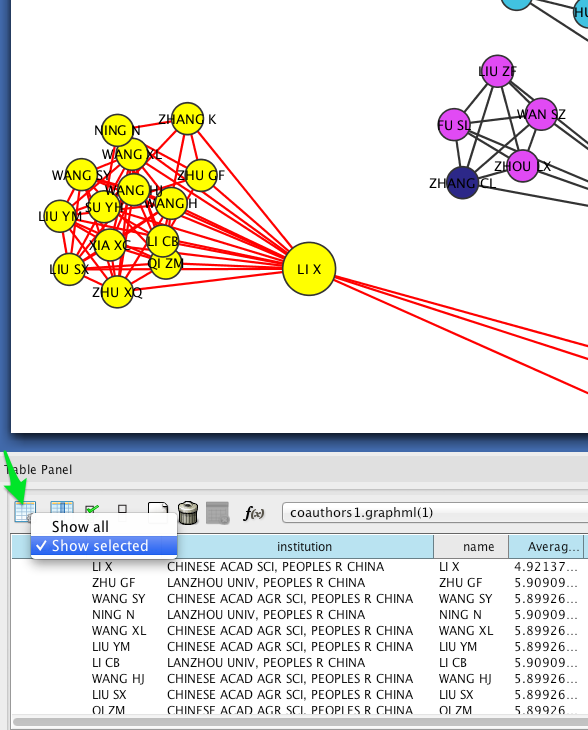
\includegraphics{coauthors.19.png}\hfill}

Circular layouts can also yield some insights into connectivity between different
institutions. In the menu bar, select \code{Layout \textgreater{} Attribute Circle Layout \textgreater{} institution}.
This should arrange the nodes in each connected component in a circle. Nodes that are
affiliated with the same institution should be adjacent to each other, so that the
circumference of each circle can be divided into regions that correspond to single
institutions. Edges crossing from one region to another should give a visual impression of
the magnitude of linkages between institutions.

{\hfill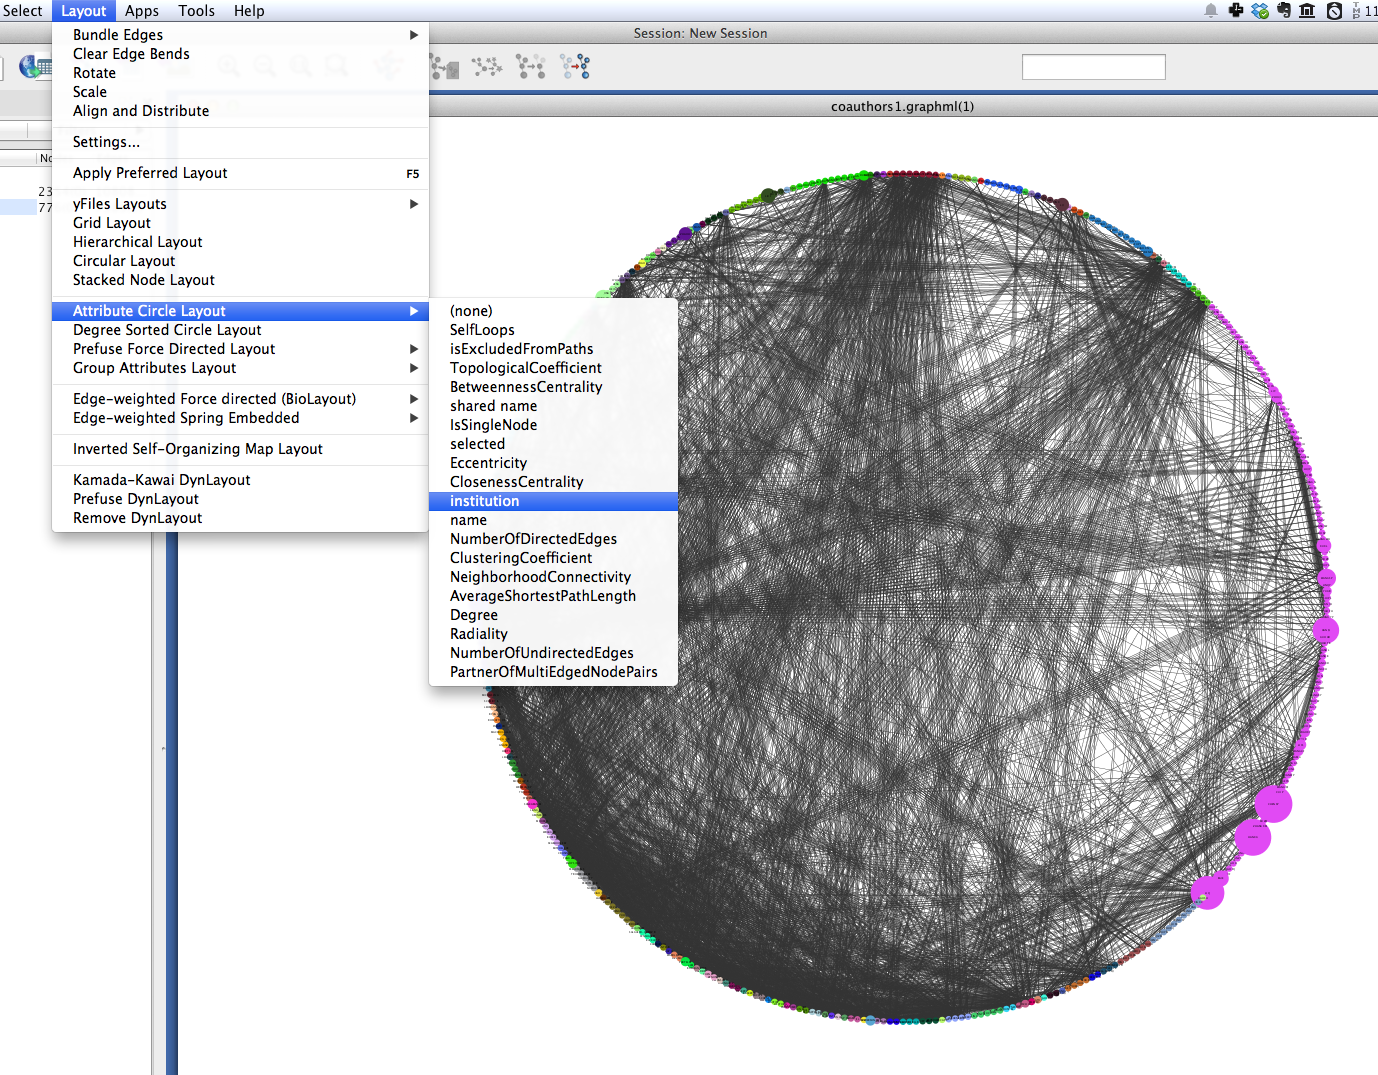
\includegraphics{coauthors.20.png}\hfill}

A similar layout, the \code{Degree Sorted Circle} layout, can yield more information about
the structure of the network. As the name suggests, this layout arranges nodes in
ascending order of degree (the number of links that each node has with other nodes in the
network). The lowest-degree nodes begin just west of due-south, and degree increases
clockwise around the circle so that the highest-degree nodes are just east of due-south.
In the network depicted below, there is extremely dense connectivity among the
highest-degree nodes, while the rest of the graph is sparse by comparison. In other words,
the most well-connected nodes are all highly connected to each other. This may be due in
part to papers with a very large number of authors.

{\hfill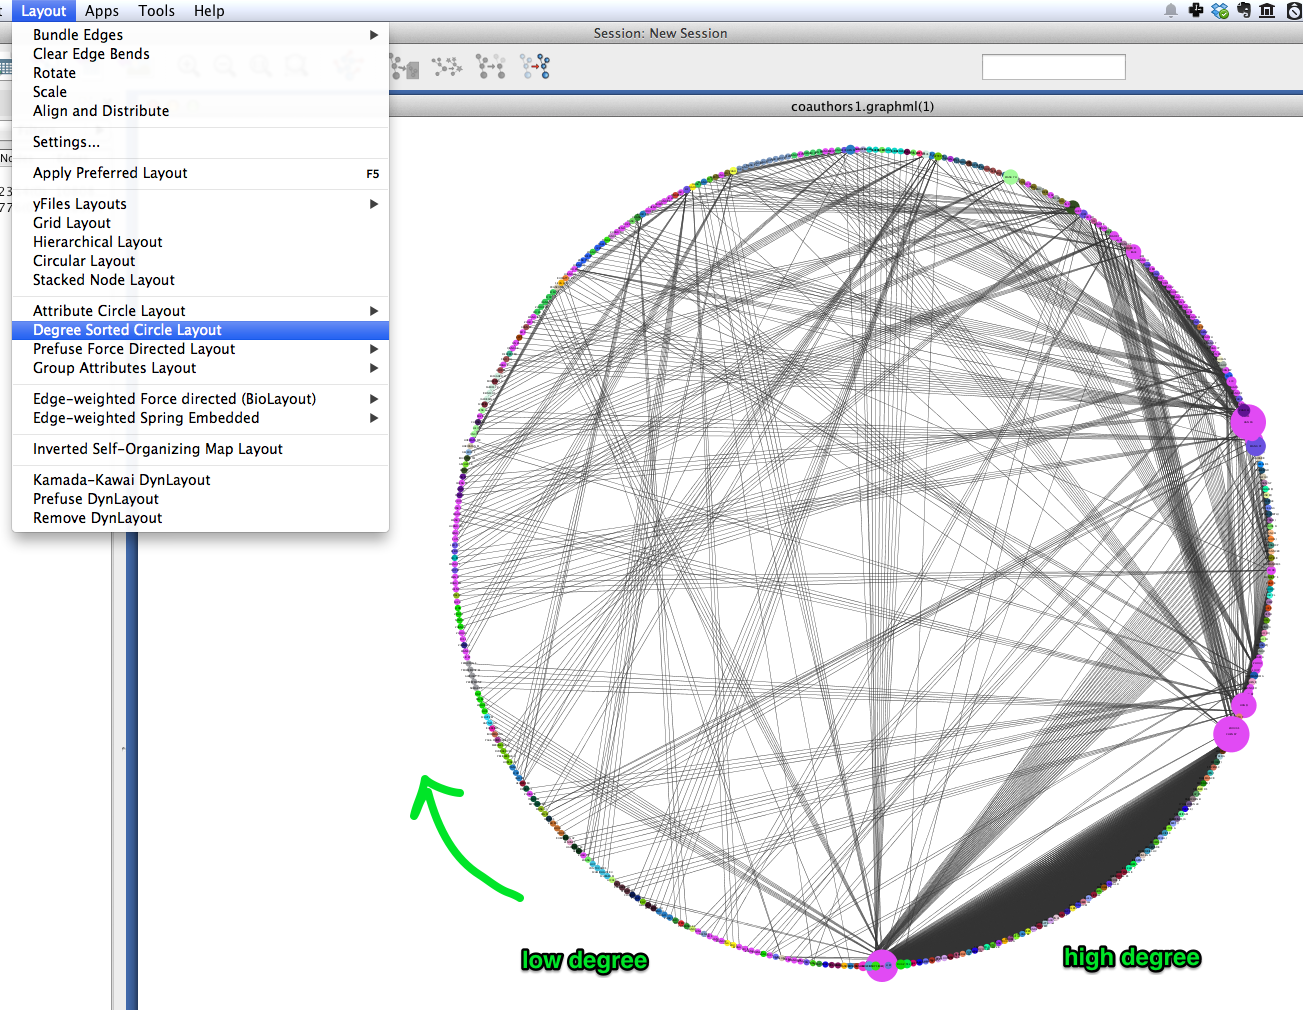
\includegraphics{coauthors.21.png}\hfill}

To export an image of your network, select
\code{File \textgreater{} Export \textgreater{} Current Network View as Graphics}, and follow the prompts to save your
image.


\paragraph{Inter-institutional Collaboration in Gephi}
\label{tutorial.coauthors:inter-institutional-collaboration-in-gephi}\label{tutorial.coauthors:coauthors-gephi}
\href{http://www.gephi.org}{Gephi} provides additional tools for analyzing coauthorship
networks. In this section, we'll use Gephi to generate an inter-institutional
collaboration network using your coauthorship network. That is, we will mash authors from
the same institutions together into institutional nodes, and combine coauthorship edges
so that we can see the magnitude of coauthorship activity between different institutions.


\subparagraph{Import \& visualize}
\label{tutorial.coauthors:import-visualize}\begin{enumerate}
\item {} 
In Gephi, select \code{File \textgreater{} Open...} and select your GraphML network file.

\item {} 
Click on the \code{Preview} tab.

\end{enumerate}

{\hfill\includegraphics{coauthors.22.png}\hfill}
\begin{enumerate}
\setcounter{enumi}{2}
\item {} 
Open the \code{Graph} window: select \code{Window \textgreater{} Graph}.

\end{enumerate}

{\hfill\includegraphics{coauthors.23.png}\hfill}
\begin{enumerate}
\setcounter{enumi}{3}
\item {} 
Open the \code{Layout} window: select \code{Window \textgreater{} Layout}.

\item {} 
In the \code{Layout} window, select the \code{Force Atlast 2 layout}, then click \code{Run}.
After a few seconds the graph should be spread out; click \code{Stop}.

\end{enumerate}

{\hfill\includegraphics{coauthors.25.png}\hfill}


\subparagraph{Partition by institution}
\label{tutorial.coauthors:partition-by-institution}\begin{enumerate}
\item {} 
Open the \code{Partition} window: select \code{Window \textgreater{} Partition}. You may need to drag the
window to the left-hand area of the Gephi workspace.

\item {} 
In the \code{Partition} window, you should be on the \code{Nodes} tab by default. Click the
green {\color{red}\bfseries{}{}`{}`}refresh’’ button, then select {\color{red}\bfseries{}{}`{}`}institution’’ from the drop-down menu. You
should see a list of all institutions.

\item {} 
To color nodes by institution, click the \code{Apply} button.

\end{enumerate}

{\hfill\includegraphics{coauthors.26.png}\hfill}

Zooming in on the network, you’ll notice that some clusters of nodes are comprised of one
or a few colors, while other clusters are quite mixed. Just as in Cytoscape, this gives a
visual impression of which research communities involve inter-institutional
collaborations, and which are more internal to a particular institution.

{\hfill\includegraphics{coauthors.27.png}\hfill}

Gephi makes it easy to collapse individual author nodes into nodes corresponding to their
institutions. Cytoscape has this feature as well, but not all of the bugs are completely
worked out.

To group authors together into their respective institutions, click the \code{Group} button
in the \code{Partition} window.

Click on the dark \textbf{T} button in the lower left corner to show node labels, and use the
right-hand slider at the bottom of the Graph window to make the labels smaller or larger.

The result may look a bit messy. There are a few things to notice:
\begin{itemize}
\item {} 
The edges between authors have been pooled into edges between institutions. The edge
weight indicates the number of coauthorship relationships between a pair of
institutions.

\item {} 
The biggest node is called \code{null}. This represents all of the authors for which no
institutional information was available. You may wish to delete this node; right-click
on the node and select \code{Delete}. When prompted, click \code{Yes}.

\end{itemize}

{\hfill\includegraphics{coauthors.28.png}\hfill}

To re-layout the network, go back to the \code{Layout} tab, and run the layout algorithm
again. You may notice that the network contracts rapidly. You may find it useful to reduce
the edge width and zoom in, to achieve a nice node-size : edge-weight ratio.

{\hfill\includegraphics{coauthors.29.png}\hfill}

To save an image of your network, click the \code{SVG/PDF/PNG} button in the lower-left
corner of the Gephi workspace.

{\hfill\includegraphics{coauthors.30.png}\hfill}


\subsubsection{Coauthorship network evolution}
\label{tutorial.coauthors:coauthorship-network-evolution}
This section describes how to generate a dynamic network with Tethne, and visualize that
network in Cytoscape. Dynamic networks allow us to go beyond analyzing the final structure
of a network, and ask how the structure of a network changes over time. In this case,
we will use a dynamic network to see how a coauthorship network grows over time.

A seemingly ubiquitous property of social networks is that they tend to be ``scale-free''.
That is, the degree distribution follows a power-law: there are a few very
highly-connected actors, and a very large number of poorly-connected actors.
The intuitive interpretation of this behavior is that ``the rich get richer.'' In other
words, if you're already popular then you're more likely to make new friends.

In this tutorial, we will visualize the impact of degree centrality on edge acquisition
by using the {\hyperref[tethne.analyze.collection:tethne.analyze.collection.attachment_probability]{\code{analyze.collection.attachment\_probability()}}} algorithm in Tethne.


\paragraph{Building a GraphCollection}
\label{tutorial.coauthors:building-a-graphcollection}
A {\hyperref[tethne.classes.graphcollection:tethne.classes.graphcollection.GraphCollection]{\code{GraphCollection}}} is a set of graphs generated from a {\hyperref[tethne.classes.corpus:tethne.classes.corpus.Corpus]{\code{Corpus}}} or model.
We can generate a GraphCollection (\code{G}) in one step, using the
\code{GraphCollection.build()} method.

A simple example might look like this:

\begin{Verbatim}[commandchars=\\\{\}]
\PYG{g+gp}{\PYGZgt{}\PYGZgt{}\PYGZgt{} }\PYG{n}{G} \PYG{o}{=} \PYG{n}{GraphCollection}\PYG{p}{(}\PYG{p}{)}\PYG{o}{.}\PYG{n}{build}\PYG{p}{(}\PYG{n}{C}\PYG{p}{,} \PYG{l+s}{\PYGZsq{}}\PYG{l+s}{date}\PYG{l+s}{\PYGZsq{}}\PYG{p}{,} \PYG{l+s}{\PYGZsq{}}\PYG{l+s}{authors}\PYG{l+s}{\PYGZsq{}}\PYG{p}{,} \PYG{l+s}{\PYGZsq{}}\PYG{l+s}{coauthors}\PYG{l+s}{\PYGZsq{}}\PYG{p}{)}
\end{Verbatim}

Here we have instructed \code{GraphCollection.build()} to build a graph for each `slice'
along the `date' axis. \code{'authors'} indicates that we want to use a graph method from
the {\hyperref[tethne.networks.authors:module-tethne.networks.authors]{\code{networks.authors}}} submodule, and \code{'coauthors'} indicates the
name of the method from that module that we wish to use.


\paragraph{Attachment Probability}
\label{tutorial.coauthors:attachment-probability}
The {\hyperref[tethne.analyze.collection:tethne.analyze.collection.attachment_probability]{\code{analyze.collection.attachment\_probability()}}} method automatically updates node
attributes in your {\hyperref[tethne.classes.graphcollection:tethne.classes.graphcollection.GraphCollection]{\code{GraphCollection}}}.

\begin{Verbatim}[commandchars=\\\{\}]
\PYG{g+gp}{\PYGZgt{}\PYGZgt{}\PYGZgt{} }\PYG{k+kn}{from} \PYG{n+nn}{tethne.analyze} \PYG{k+kn}{import} \PYG{n}{collection}
\PYG{g+gp}{\PYGZgt{}\PYGZgt{}\PYGZgt{} }\PYG{n}{collection}\PYG{o}{.}\PYG{n}{attachment\PYGZus{}probability}\PYG{p}{(}\PYG{n}{C}\PYG{p}{)}
\end{Verbatim}


\paragraph{Dynamic XGMML}
\label{tutorial.coauthors:dynamic-xgmml}
Use the {\hyperref[tethne.writers.collection:tethne.writers.collection.to_dxgmml]{\code{writers.collection.to\_dxgmml()}}} method to create a \href{https://code.google.com/p/dynnetwork/wiki/DynamicXGMML}{dynamic XGMML} network data file.

\begin{Verbatim}[commandchars=\\\{\}]
\PYG{g+gp}{\PYGZgt{}\PYGZgt{}\PYGZgt{} }\PYG{k+kn}{from} \PYG{n+nn}{tethne.writers} \PYG{k+kn}{import} \PYG{n}{collection}
\PYG{g+gp}{\PYGZgt{}\PYGZgt{}\PYGZgt{} }\PYG{n}{collection}\PYG{o}{.}\PYG{n}{to\PYGZus{}dxgmml}\PYG{p}{(}\PYG{n}{G}\PYG{p}{,} \PYG{l+s}{\PYGZsq{}}\PYG{l+s}{/path/to/my/dynamicnetwork.xgmml}\PYG{l+s}{\PYGZsq{}}\PYG{p}{)}
\end{Verbatim}


\paragraph{Cytoscape}
\label{tutorial.coauthors:id16}
In Cytoscape, import your .xgmml file by selecting
\code{File \textgreater{} Import \textgreater{} Dynamic Network \textgreater{} XGMML File...}. Apply a force-directed or
spring-embedded layout.

{\hfill\includegraphics{coauthors.34.png}\hfill}

In the VizMapper, map \code{Node Size} to \code{attachment\_probability}.

{\hfill\includegraphics{coauthors.35.png}\hfill}

Double-click on the function icon next to \code{Current Mapping} to edit the \code{Node Size}
mapping function.
\begin{enumerate}
\item {} 
Click the \code{Min/Max} button, and set the maximum value to \code{1.0}.

\item {} 
Slick on the \code{Add} button to create a new handle at an intermediate value. Drag
the red open box up, and drag the corresponding black arrow left and right to alter
the mapping function.

\item {} 
Click \code{OK}.

\end{enumerate}

{\hfill\includegraphics{coauthors.36.png}\hfill}

In the Control Panel, select the \code{Dynamic Network} tab.
\begin{enumerate}
\item {} 
Set the time resolution to roughly match the time-range of your network. In the
example below, the network covers about 35 years, so a resolution of 1/50 was selected.

\item {} 
Set \code{Time smoothness} to \code{0 ms}.

\item {} 
Use the slider to move through the states of your dynamic network. To view all states
in succession, use the \code{\textless{}\textless{} Play} and \code{Play \textgreater{}\textgreater{}} buttons.

\end{enumerate}

{\hfill\includegraphics{coauthors.37.png}\hfill}

The size of each node should reflect the relative probability that a node will accrue a
new neighbor in the next time slice. Try zooming in on a particular region of your
network, and move between two successive states to verify that this is the case.

{\hfill\includegraphics{coauthors.38.png}\hfill}


\subsection{Co-citation Analysis}
\label{tutorial.cocitation:co-citation-analysis}\label{tutorial.cocitation::doc}\setbox0\vbox{
\begin{minipage}{0.95\linewidth}
\begin{itemize}
\item {} 
{\hyperref[tutorial.cocitation:getting-started]{Getting Started}}

\item {} 
{\hyperref[tutorial.cocitation:reading-wos-data]{Reading WoS Data}}

\item {} 
{\hyperref[tutorial.cocitation:building-a-co-citation-graphcollection]{Building a Co-citation GraphCollection}}
\begin{itemize}
\item {} 
{\hyperref[tutorial.cocitation:slicing-a-corpus]{Slicing a Corpus}}

\item {} 
{\hyperref[tutorial.cocitation:time-variant-co-citation-graph]{Time-variant co-citation graph}}

\end{itemize}

\item {} 
{\hyperref[tutorial.cocitation:analyzing-the-graphcollection]{Analyzing the GraphCollection}}
\begin{itemize}
\item {} 
{\hyperref[tutorial.cocitation:id1]{Betweenness centrality}}

\item {} 
{\hyperref[tutorial.cocitation:burstness]{Burstness}}

\item {} 
{\hyperref[tutorial.cocitation:sigma]{Sigma}}

\end{itemize}

\end{itemize}
\end{minipage}}
\begin{center}\setlength{\fboxsep}{5pt}\shadowbox{\box0}\end{center}

\begin{notice}{note}{Note:}
This tutorial was developed for the course \href{http://devo-evo.lab.asu.edu/methods}{Introduction to Digital \&
Computational Methods in the Humanities (HPS)},
created and taught by \href{http://devo-evo.lab.asu.edu/?q=damerow}{Julia Damerow} and
\href{http://gradinfo.cbs.asu.edu/?page\_id=49}{Erick Peirson}.
\end{notice}

Co-citation analysis gained popularity in the 1970s as a technique for ``mapping''
scientific literatures, and for finding latent semantic relationships among technical
publications.

Two papers are co-cited if they are both cited by the same, third, paper. The standard
approach to co-citation analysis is to generate a sample of bibliographic records from a
particular field by using certain keywords or journal names, and then build a co-citation
graph describing relationships among their cited references. Thus the majority of papers
that are represented as nodes in the co-citation graph are \textbf{not} papers that responded
to the selection criteria used to build the dataset.

{\hfill\includegraphics{citationnetworks.png}\hfill}

Our objective in this tutorial is to identify papers that bridge the gap between
otherwise disparate areas of knowledge in the scientific literature. In this tutorial, we
rely on the theoretical framework described in \href{http://cluster.cis.drexel.edu/~cchen/citespace/doc/jasist2006.pdf}{Chen (2006)} and \href{http://arxiv.org/pdf/0904.1439.pdf}{Chen et al.
(2009)}.

According to Chen, we can detect potentially transformative changes in scientific
knowledge by looking for cited references that both (a) rapidly accrue citations, and (b)
have high betweenness-centrality in a co-citation network. It helps if we think of each
scientific paper as representing a ``concept'' (its core knowledge claim, perhaps), and a
co-citation event as representing a proposition connecting two concepts in the
knowledge-base of a scientific field. If a new paper emerges that is highly co-cited with
two otherwise-distinct clusters of concepts, then that might mean that the field is
adopting new concepts and propositions in a way that is structurally radical for their
conceptual framework.

\href{http://arxiv.org/pdf/0904.1439.pdf}{Chen (2009)} introduces sigma (\(\Sigma\)) as a
metric for potentially transformative cited references:
\begin{gather}
\begin{split}\Sigma(v) = (g(v) + 1)^{burstness(v)}\end{split}\notag
\end{gather}
...where the \href{http://en.wikipedia.org/wiki/Betweenness\_centrality}{betweenness centrality} of each node \(v\) is:
\begin{gather}
\begin{split}g(v) = \sum\limits_{i\neq j\neq v} \frac{\sigma_{ij} (v)}{\sigma_{ij}}\end{split}\notag
\end{gather}
...where \(\sigma_{ij}\) is the number of shortest paths from node \emph{i} to node
\emph{j} and \(\sigma_{ij}(v)\) is the number of those paths that pass through \emph{v}.

\(burstness\) (0.-1. normalized) is estimated using \href{http://www.cs.cornell.edu/home/kleinber/bhs.pdf}{Kleingberg's (2002)} automaton model.

First, we'll build a time-variant co-citation network. We'll then use Chen's sigma
(\(\Sigma\)) metric to identify potential turning-points in our corpus.


\subsubsection{Getting Started}
\label{tutorial.cocitation:getting-started}
Before you begin, be sure to install the latest version of Tethne. Consult the
\emph{installation} guide for details.

\textbf{If you run into problems}, don't panic. Tethne is under active development, and there
are certainly bugs to be found. Please report any problems, including errors in this
tutorial, via our \href{https://github.com/diging/tethne/issues?state=open}{GitHub issue tracker}.

For this tutorial, you'll need some citation data from the ISI Web of Science. If this is
your first time working with WoS citation data, check out {\hyperref[tutorial.getting_data:gettingdata]{\emph{Getting Bibliographic Data}}}. We'll
assume that you have downloaded a few sets of records from WoS, and stored them all in
the same directory.

\begin{Verbatim}[commandchars=\\\{\}]
\PYG{g+gp}{\PYGZgt{}\PYGZgt{}\PYGZgt{} }\PYG{n}{datapath} \PYG{o}{=} \PYG{l+s}{\PYGZsq{}}\PYG{l+s}{/path/to/my/data/directory}\PYG{l+s}{\PYGZsq{}}
\end{Verbatim}


\subsubsection{Reading WoS Data}
\label{tutorial.cocitation:reading-wos-data}
You can parse WoS data from one or multiple field-tagged data files, using the methods
in the {\hyperref[tethne.readers:module-tethne.readers]{\code{readers}}} module. Since we're working with multiple data files, we'll
use the \code{readers.wos.corpus\_from\_dir} method to parse the WoS data and create
a new {\hyperref[tethne.classes.corpus:tethne.classes.corpus.Corpus]{\code{Corpus}}} called \code{MyCorpus}.

\begin{Verbatim}[commandchars=\\\{\}]
\PYG{g+gp}{\PYGZgt{}\PYGZgt{}\PYGZgt{} }\PYG{k+kn}{from} \PYG{n+nn}{tethne.readers} \PYG{k+kn}{import} \PYG{n}{wos}
\PYG{g+gp}{\PYGZgt{}\PYGZgt{}\PYGZgt{} }\PYG{n}{MyCorpus} \PYG{o}{=} \PYG{n}{wos}\PYG{o}{.}\PYG{n}{corpus\PYGZus{}from\PYGZus{}dir}\PYG{p}{(}\PYG{n}{datapath}\PYG{p}{)}
\end{Verbatim}

\code{MyCorpus} should contain some {\hyperref[tethne.classes.paper:tethne.classes.paper.Paper]{\code{Paper}}}s, as well as some citations.

\begin{Verbatim}[commandchars=\\\{\}]
\PYG{g+gp}{\PYGZgt{}\PYGZgt{}\PYGZgt{} }\PYG{k}{print} \PYG{n+nb}{len}\PYG{p}{(}\PYG{n}{MyCorpus}\PYG{o}{.}\PYG{n}{papers}\PYG{p}{)}       \PYG{c}{\PYGZsh{} How many Papers?}
\PYG{g+go}{1859}
\PYG{g+gp}{\PYGZgt{}\PYGZgt{}\PYGZgt{} }\PYG{k}{print} \PYG{n+nb}{len}\PYG{p}{(}\PYG{n}{MyCorpus}\PYG{o}{.}\PYG{n}{citations}\PYG{p}{)}    \PYG{c}{\PYGZsh{} How many citations?}
\PYG{g+go}{57774}
\end{Verbatim}

If you have fewer {\hyperref[tethne.classes.paper:tethne.classes.paper.Paper]{\code{Paper}}}s than you expect, it is possible that some of the
records in your dataset were duplicates. If you don't have any citations, go back
and make sure that you downloaded full records with citations from the WoS database. See
{\hyperref[tutorial.getting_data:gettingdata]{\emph{Getting Bibliographic Data}}}.


\subsubsection{Building a Co-citation GraphCollection}
\label{tutorial.cocitation:building-a-co-citation-graphcollection}

\paragraph{Slicing a Corpus}
\label{tutorial.cocitation:slicing-a-corpus}
Think of slicing as indexing: we will divide the {\hyperref[tethne.classes.paper:tethne.classes.paper.Paper]{\code{Paper}}}s in our {\hyperref[tethne.classes.corpus:tethne.classes.corpus.Corpus]{\code{Corpus}}}
into bins by publication date, so that later on we can retrieve sets of papers
corresponding to particular time-periods. You can slice your data using the
\code{Corpus.slice()} method.

In this tutorial, we'll slice our {\hyperref[tethne.classes.corpus:tethne.classes.corpus.Corpus]{\code{Corpus}}} into two-year subsets using the
``time\_period'' method.
\begin{figure}[htbp]
\centering
\capstart

\includegraphics{timeline.timeslice.png}
\caption{\textbf{Time-period} slicing, with a window-size of 4 years.}\end{figure}
\begin{figure}[htbp]
\centering
\capstart

\includegraphics{timeline.timewindow.png}
\caption{\textbf{Time-window} slicing, with a window-size of 4 years and a step-size of 1 year.}\end{figure}

\begin{Verbatim}[commandchars=\\\{\}]
\PYG{g+gp}{\PYGZgt{}\PYGZgt{}\PYGZgt{} }\PYG{n}{MyCorpus}\PYG{o}{.}\PYG{n}{slice}\PYG{p}{(}\PYG{l+s}{\PYGZsq{}}\PYG{l+s}{date}\PYG{l+s}{\PYGZsq{}}\PYG{p}{,} \PYG{l+s}{\PYGZsq{}}\PYG{l+s}{time\PYGZus{}period}\PYG{l+s}{\PYGZsq{}}\PYG{p}{,} \PYG{n}{window\PYGZus{}size}\PYG{o}{=}\PYG{l+m+mi}{2}\PYG{p}{)}
\end{Verbatim}

\begin{Verbatim}[commandchars=\\\{\}]
\end{Verbatim}


\paragraph{Time-variant co-citation graph}
\label{tutorial.cocitation:time-variant-co-citation-graph}
We will use the \code{GraphCollection.build()} method to generate a cocitation
{\hyperref[tethne.classes.graphcollection:tethne.classes.graphcollection.GraphCollection]{\code{GraphCollection}}}.

The \code{methods\_kw} parameter lets us set keyword arguments for the
{\hyperref[tethne.networks.papers:tethne.networks.papers.cocitation]{\code{networks.papers.cocitation()}}} graph builder. \code{threshold} sets the minimum
number of cocitations for an edge to be included in the graph. \code{topn} sets the number
of top-cited nodes to include in each time-slice.

\begin{Verbatim}[commandchars=\\\{\}]
\PYG{g+gp}{\PYGZgt{}\PYGZgt{}\PYGZgt{} }\PYG{k+kn}{from} \PYG{n+nn}{tethne} \PYG{k+kn}{import} \PYG{n}{GraphCollection}
\PYG{g+gp}{\PYGZgt{}\PYGZgt{}\PYGZgt{} }\PYG{n}{kw} \PYG{o}{=} \PYG{p}{\PYGZob{}} \PYG{l+s}{\PYGZsq{}}\PYG{l+s}{threshold}\PYG{l+s}{\PYGZsq{}}\PYG{p}{:} \PYG{l+m+mi}{2}\PYG{p}{,} \PYG{l+s}{\PYGZsq{}}\PYG{l+s}{topn}\PYG{l+s}{\PYGZsq{}}\PYG{p}{:} \PYG{l+m+mi}{200} \PYG{p}{\PYGZcb{}}
\PYG{g+gp}{\PYGZgt{}\PYGZgt{}\PYGZgt{} }\PYG{n}{G} \PYG{o}{=} \PYG{n}{GraphCollection}\PYG{p}{(}\PYG{p}{)}\PYG{o}{.}\PYG{n}{build}\PYG{p}{(}\PYG{n}{MyCorpus}\PYG{p}{,} \PYG{l+s}{\PYGZsq{}}\PYG{l+s}{date}\PYG{l+s}{\PYGZsq{}}\PYG{p}{,} \PYG{l+s}{\PYGZsq{}}\PYG{l+s}{papers}\PYG{l+s}{\PYGZsq{}}\PYG{p}{,} \PYG{l+s}{\PYGZsq{}}\PYG{l+s}{cocitation}\PYG{l+s}{\PYGZsq{}}\PYG{p}{,} \PYG{n}{method\PYGZus{}kwargs}\PYG{o}{=}\PYG{n}{kw}\PYG{p}{)}
\end{Verbatim}


\subsubsection{Analyzing the GraphCollection}
\label{tutorial.cocitation:analyzing-the-graphcollection}
According to the equation for sigma (\(\Sigma\)) given above, we need to calculate
the betweenness centrality and the burstness of each node over time. The
\code{analyze.cocitation.sigma()} method will do both of these things for us, as
described further down in this tutorial. For the sake of illustration, however, we'll walk
through the intermediate steps.


\paragraph{Betweenness centrality}
\label{tutorial.cocitation:id1}
Betweenness centrality \(g(v)\) is a measure of the structural importance of a node in
a graph. Formally, betweenness centrality is a measure of the number of shortest paths
that pass through a particular node. A node with high betweenness centrality tends to
connect disparate regions of a graph, linking clusters that might otherwise be
disconnected.
\begin{gather}
\begin{split}g(v) = \sum\limits_{i\neq j\neq v} \frac{\sigma_{ij} (v)}{\sigma_{ij}}\end{split}\notag
\end{gather}
...where \(\sigma_{ij}\) is the number of shortest paths from node \emph{i} to node
\emph{j} and \(\sigma_{ij}(v)\) is the number of those paths that pass through \emph{v}.

We can calculate the centrality of all nodes in each of the graphs in our
{\hyperref[tethne.classes.graphcollection:tethne.classes.graphcollection.GraphCollection]{\code{GraphCollection}}} using the {\hyperref[tethne.analyze.collection:tethne.analyze.collection.algorithm]{\code{analyze.collection.algorithm()}}} method:

\begin{Verbatim}[commandchars=\\\{\}]
\PYG{g+gp}{\PYGZgt{}\PYGZgt{}\PYGZgt{} }\PYG{k+kn}{from} \PYG{n+nn}{tethne.analyze} \PYG{k+kn}{import} \PYG{n}{collection}
\PYG{g+gp}{\PYGZgt{}\PYGZgt{}\PYGZgt{} }\PYG{n}{bc} \PYG{o}{=} \PYG{n}{collection}\PYG{o}{.}\PYG{n}{algorithm}\PYG{p}{(}\PYG{n}{G}\PYG{p}{,} \PYG{l+s}{\PYGZsq{}}\PYG{l+s}{betweenness\PYGZus{}centrality}\PYG{l+s}{\PYGZsq{}}\PYG{p}{)}
\end{Verbatim}

\code{bc} is a dictionary of centrality values, nested like:
\code{\{ slice : \{ node : centrality \} \}}.

The nodes in our {\hyperref[tethne.classes.graphcollection:tethne.classes.graphcollection.GraphCollection]{\code{GraphCollection}}} (\code{G}) are also updated with their centrality
values.


\paragraph{Burstness}
\label{tutorial.cocitation:burstness}
\href{http://www.cs.cornell.edu/home/kleinber/bhs.pdf}{Kleingberg's (2002)} burstness model
is a popular approach for detecting ``busts'' of interest or activity in streams of data
(e.g. identifying trending terms in Twitter feeds). Chen (2009) suggests that we apply
this model to citations. The idea is that the (observed) frequency with which a reference
is cited is a product of an (unobserved) level or state of interest surrounding that
citation. Kleinberg uses a hidden \href{http://en.wikipedia.org/wiki/Hidden\_Markov\_model}{hidden markov model} to infer the most likely sequence of
``burstness'' states for an event (a cited reference, in our case) over time. His algorithm
is implemented in {\hyperref[tethne.analyze.corpus:tethne.analyze.corpus.feature_burstness]{\code{analyze.corpus.feature\_burstness()}}}, and can be used for any
feature in our {\hyperref[tethne.classes.corpus:tethne.classes.corpus.Corpus]{\code{Corpus}}}.

Since citations are features in our {\hyperref[tethne.classes.corpus:tethne.classes.corpus.Corpus]{\code{Corpus}}}, we can use the
{\hyperref[tethne.analyze.corpus:tethne.analyze.corpus.burstness]{\code{analyze.corpus.burstness()}}} method to get the burstness profiles for the
top-cited reference in our dataset.

\begin{Verbatim}[commandchars=\\\{\}]
\PYG{g+gp}{\PYGZgt{}\PYGZgt{}\PYGZgt{} }\PYG{k+kn}{from} \PYG{n+nn}{tethne.analyze} \PYG{k+kn}{import} \PYG{n}{corpus}
\PYG{g+gp}{\PYGZgt{}\PYGZgt{}\PYGZgt{} }\PYG{n}{B} \PYG{o}{=} \PYG{n}{corpus}\PYG{o}{.}\PYG{n}{burstness}\PYG{p}{(}\PYG{n}{MyCorpus}\PYG{p}{,} \PYG{l+s}{\PYGZsq{}}\PYG{l+s}{citations}\PYG{l+s}{\PYGZsq{}}\PYG{p}{,} \PYG{n}{topn}\PYG{o}{=}\PYG{l+m+mi}{2}\PYG{p}{,} \PYG{n}{perslice}\PYG{o}{=}\PYG{n+nb+bp}{True}\PYG{p}{)}
\PYG{g+gp}{\PYGZgt{}\PYGZgt{}\PYGZgt{} }\PYG{n}{B}\PYG{p}{[}\PYG{l+s}{\PYGZsq{}}\PYG{l+s}{BIOLOGY MR 2009 NATURE}\PYG{l+s}{\PYGZsq{}}\PYG{p}{]}
\PYG{g+go}{([2009, 2010, 2011, 2012, 2013], [0., 0.4, 0.6, 0.2, 0.])}
\end{Verbatim}

\code{perslice=True} tells Tethne to get the \code{topn=2} most cited references for each
slice in \code{MyCorpus}. \code{burstness()} returns a dictionary, \code{B}; the keys are our cited
references, and the values are \code{(dates,burstness)} tuples for each reference.

Burstness values are normalized with respect to the highest possible burstness state. In
other words, a burstness of 1.0 corresponds to the highest possible state. We can control
the number of states by adding the keyword argument \code{k}, for example:

\begin{Verbatim}[commandchars=\\\{\}]
\PYG{g+gp}{\PYGZgt{}\PYGZgt{}\PYGZgt{} }\PYG{n}{B} \PYG{o}{=} \PYG{n}{corpus}\PYG{o}{.}\PYG{n}{burstness}\PYG{p}{(}\PYG{n}{MyCorpus}\PYG{p}{,} \PYG{l+s}{\PYGZsq{}}\PYG{l+s}{citations}\PYG{l+s}{\PYGZsq{}}\PYG{p}{,} \PYG{n}{topn}\PYG{o}{=}\PYG{l+m+mi}{2}\PYG{p}{,} \PYG{n}{perslice}\PYG{o}{=}\PYG{n+nb+bp}{True}\PYG{p}{,} \PYG{n}{k}\PYG{o}{=}\PYG{l+m+mi}{10}\PYG{p}{)}
\end{Verbatim}

The {\hyperref[tethne.analyze.corpus:module-tethne.analyze.corpus]{\code{analyze.corpus}}} module also provides a simple way to visualize the burstness
of our cited references: {\hyperref[tethne.analyze.corpus:tethne.analyze.corpus.plot_burstness]{\code{analyze.corpus.plot\_burstness()}}}.

\begin{Verbatim}[commandchars=\\\{\}]
\PYG{g+gp}{\PYGZgt{}\PYGZgt{}\PYGZgt{} }\PYG{k+kn}{from} \PYG{n+nn}{tethne.analyze.corpus} \PYG{k+kn}{import} \PYG{n}{burstness}
\PYG{g+gp}{\PYGZgt{}\PYGZgt{}\PYGZgt{} }\PYG{n}{fig} \PYG{o}{=} \PYG{n}{plot\PYGZus{}burstness}\PYG{p}{(}\PYG{n}{MyCorpus}\PYG{p}{,} \PYG{l+s}{\PYGZsq{}}\PYG{l+s}{citations}\PYG{l+s}{\PYGZsq{}}\PYG{p}{,} \PYG{n}{topn}\PYG{o}{=}\PYG{l+m+mi}{2}\PYG{p}{,} \PYG{n}{perslice}\PYG{o}{=}\PYG{n+nb+bp}{True}\PYG{p}{)}
\PYG{g+gp}{\PYGZgt{}\PYGZgt{}\PYGZgt{} }\PYG{n}{fig}\PYG{o}{.}\PYG{n}{savefig}\PYG{p}{(}\PYG{l+s}{\PYGZsq{}}\PYG{l+s}{\PYGZti{}/burstness.png}\PYG{l+s}{\PYGZsq{}}\PYG{p}{)}
\end{Verbatim}

Years prior to the first occurrence of each feature are grayed out. Periods
in which the feature was bursty are depicted by colored blocks, the opacity
of which indicates burstness intensity.
\begin{figure}[htbp]
\centering

\includegraphics{burstness.png}
\end{figure}


\paragraph{Sigma}
\label{tutorial.cocitation:sigma}
\href{http://arxiv.org/pdf/0904.1439.pdf}{Chen (2009)} proposed sigma (\(\Sigma\)) as a
metric for potentially transformative cited references:
\begin{gather}
\begin{split}\Sigma(v) = (g(v) + 1)^{burstness(v)}\end{split}\notag
\end{gather}
The module \code{analyze.cocitation} provides methods for calculating \(\Sigma\)
from a cocitation {\hyperref[tethne.classes.graphcollection:tethne.classes.graphcollection.GraphCollection]{\code{GraphCollection}}} and a {\hyperref[tethne.classes.corpus:tethne.classes.corpus.Corpus]{\code{Corpus}}} in one step.

The method \code{analyze.plot\_sigma()} calculates \(\Sigma\) for each node in each
time-slice of our {\hyperref[tethne.classes.graphcollection:tethne.classes.graphcollection.GraphCollection]{\code{GraphCollection}}}, and also generates a figure that shows
values for the top nodes in each slice.

\begin{Verbatim}[commandchars=\\\{\}]
\PYG{g+gp}{\PYGZgt{}\PYGZgt{}\PYGZgt{} }\PYG{k+kn}{from} \PYG{n+nn}{tethne.analyze.cocitation} \PYG{k+kn}{import} \PYG{n}{plot\PYGZus{}sigma}
\PYG{g+gp}{\PYGZgt{}\PYGZgt{}\PYGZgt{} }\PYG{n}{fig}\PYG{p}{,}\PYG{n}{G} \PYG{o}{=} \PYG{n}{plot\PYGZus{}sigma}\PYG{p}{(}\PYG{n}{G}\PYG{p}{,} \PYG{n}{MyCorpus}\PYG{p}{,} \PYG{n}{topn}\PYG{o}{=}\PYG{l+m+mi}{5}\PYG{p}{,} \PYG{n}{perslice}\PYG{o}{=}\PYG{n+nb+bp}{True}\PYG{p}{)}
\PYG{g+gp}{\PYGZgt{}\PYGZgt{}\PYGZgt{} }\PYG{n}{fig}\PYG{o}{.}\PYG{n}{savefig}\PYG{p}{(}\PYG{l+s}{\PYGZsq{}}\PYG{l+s}{\PYGZti{}/sigma\PYGZus{}plot.png}\PYG{l+s}{\PYGZsq{}}\PYG{p}{)}
\end{Verbatim}

In the figure below, the top 5 most sigma-influential nodes in each slice are shown. Red
bands indicate periods in which each paper had a high \(\Sigma\); opacity indicates
the intensity of \(\Sigma\) (normalized by the highest value in the plot). Those red
bands suggest points at which that particular paper may have significantly altered the
conceptual framework of the field represented by our corpus.
\begin{figure}[htbp]
\centering

\includegraphics{sigma_plot.png}
\end{figure}

In the last step, the nodes in \code{G} were also updated with \(\Sigma\) values. We can
write our {\hyperref[tethne.classes.graphcollection:tethne.classes.graphcollection.GraphCollection]{\code{GraphCollection}}} as a dynamic graph for visualization in Cytoscape
using the {\hyperref[tethne.writers.collection:tethne.writers.collection.to_dxgmml]{\code{writers.collection.to\_dxgmml()}}} method:

\begin{Verbatim}[commandchars=\\\{\}]
\PYG{g+gp}{\PYGZgt{}\PYGZgt{}\PYGZgt{} }\PYG{k+kn}{from} \PYG{n+nn}{tethne.writers} \PYG{k+kn}{import} \PYG{n}{collection}
\PYG{g+gp}{\PYGZgt{}\PYGZgt{}\PYGZgt{} }\PYG{n}{collection}\PYG{o}{.}\PYG{n}{to\PYGZus{}dxgmml}\PYG{p}{(}\PYG{n}{G}\PYG{p}{,} \PYG{l+s}{\PYGZsq{}}\PYG{l+s}{\PYGZti{}/cocitation.xgmml}\PYG{l+s}{\PYGZsq{}}\PYG{p}{)}
\end{Verbatim}

In the visualization below, node and label sizes are mapped to \(\Sigma\), and border
width is mapped to the number of citations for each respective node in each slice.
\begin{figure}[htbp]
\centering

\includegraphics{cocitation_sigma2.png}
\end{figure}


\subsection{Geographic Networks}
\label{tutorial.geonetworks:geographic-networks}\label{tutorial.geonetworks::doc}\setbox0\vbox{
\begin{minipage}{0.95\linewidth}
\begin{itemize}
\item {} 
{\hyperref[tutorial.geonetworks:requirements]{Requirements}}

\item {} 
{\hyperref[tutorial.geonetworks:are-your-data-suitable]{Are your data suitable?}}

\item {} 
{\hyperref[tutorial.geonetworks:coauthorship-network-with-geocoding]{Coauthorship network with geocoding}}

\item {} 
{\hyperref[tutorial.geonetworks:export-to-graphml]{Export to GraphML}}

\item {} 
{\hyperref[tutorial.geonetworks:geo-layout-in-gephi]{Geo Layout in Gephi}}

\item {} 
{\hyperref[tutorial.geonetworks:eigenvector-centrality]{Eigenvector Centrality}}

\item {} 
{\hyperref[tutorial.geonetworks:plotting-geodata-on-a-basemap]{Plotting geodata on a basemap}}
\begin{itemize}
\item {} 
{\hyperref[tutorial.geonetworks:node-size-attribute]{Node size attribute}}

\item {} 
{\hyperref[tutorial.geonetworks:exporting-kml-kmz]{Exporting KML (KMZ)}}

\item {} 
{\hyperref[tutorial.geonetworks:visualization-in-google-earth]{Visualization in Google Earth}}

\end{itemize}

\end{itemize}
\end{minipage}}
\begin{center}\setlength{\fboxsep}{5pt}\shadowbox{\box0}\end{center}

\begin{notice}{note}{Note:}
This tutorial was developed for the course \href{http://devo-evo.lab.asu.edu/methods}{Introduction to Digital \&
Computational Methods in the Humanities (HPS)},
created and taught by \href{http://devo-evo.lab.asu.edu/?q=damerow}{Julia Damerow} and
\href{http://gradinfo.cbs.asu.edu/?page\_id=49}{Erick Peirson}.
\end{notice}

Many bibliographic datasets include institutional affiliations for authors. Using
geocoding services, such as the \href{https://developers.google.com/maps/documentation/geocoding/}{Google Geocoding API}, we can convert
institution names and addresses into geographic coordinates that can be plotted on a map.
Tethne provides geocoding services in the {\hyperref[tethne.services.geocode:module-tethne.services.geocode]{\code{services.geocode}}} module.

In this tutorial, we will use the Google Geocoding service to obtain geographic
coordinates for authors in a coauthorship network (see {\hyperref[tutorial.coauthors:coauthorship]{\emph{Coauthorship Networks}}}) and its
derivative, the institutions network (see {\hyperref[tethne.networks.authors:tethne.networks.authors.institutions]{\code{networks.authors.institutions()}}}). We
will then plot those geo-coded networks in Gephi using the Geo Layout plugin, and overlay
them on a 3D map of the globe in Google Earth.

The examples in this tutorial were generated using records for the journal \emph{Ecology} from
2001-2013. See {\hyperref[tutorial.getting_data:gettingdata]{\emph{Getting Bibliographic Data}}}.


\subsubsection{Requirements}
\label{tutorial.geonetworks:requirements}
The Python package \href{https://code.google.com/p/geopy/}{geopy} must be installed and in
your Python path. You should be able to install it using:

\begin{Verbatim}[commandchars=\\\{\}]
\PYG{n+nv}{\PYGZdl{} }pip install geopy
\end{Verbatim}


\subsubsection{Are your data suitable?}
\label{tutorial.geonetworks:are-your-data-suitable}
Not all bibliographic data is amenable to geocoding. When parsing data from the Web of
Science, Tethne looks for author institutional affiliations in the \code{C1} field. For
example:

\begin{Verbatim}[commandchars=\\\{\}]
C1 [Keung, Jacky] Hong Kong Polytech Univ, Dept Comp, Kowloon, Hong Kong, Peoples R China.
   [Kocaguneli, Ekrem; Menzies, Tim] W Virginia Univ, Lane Dept Comp Sci \PYGZam{} Elect Engn, Morgantown, WV 26505 USA.
\end{Verbatim}

Visually inspect your Web of Science data before proceeding. If most of your data lack the
C1 field, then attempting to geocode a coauthorship network based on these data won't
be particularly fruitful. Try downloading a dataset that contains more recently-published
records.

Since the Web of Science does not use controlled sub-fields for institution addresses,
Tethne pays attention only to the first and last parts of each affiliation field. From
Tethne's perspective, then, the mapping between authors and institutions shown above
becomes:

\begin{tabulary}{\linewidth}{|L|L|}
\hline
\textsf{\relax 
Author
} & \textsf{\relax 
Institution
}\\
\hline
KEUNG J
 & 
HONG KONG POLYTECH UNIV, PEOPLES R CHINA
\\

KOCAGUNELI E
 & 
W VIRGINIA UNIV, WV 26505 USA
\\

MENZIES T
 & 
W VIRGINIA UNIV, WV 26505 USA
\\
\hline\end{tabulary}


When attempting to retrieve geographic information for these institutions, Tethne first
attempts to retrieve a location for the institution itself, e.g. by passing \code{HONG KONG
POLYTECH UNIV, PEOPLES R CHINA} to the geocoding service. If this does not yield a
result, Tethne tries passing the last field only, e.g. \code{PEOPLES R CHINA}. Note that for
most U.S. addresses, the state and zip code are included in the last field, e.g. \code{WV
26505 USA}. The method that successfully yielded a geographic result determines the
\code{precision} field, discussed below.


\subsubsection{Coauthorship network with geocoding}
\label{tutorial.geonetworks:coauthorship-network-with-geocoding}
The {\hyperref[tethne.networks.authors:tethne.networks.authors.coauthors]{\code{networks.authors.coauthors()}}} method accepts a boolean keyword argument called
\code{geocode}. If \code{geocode} is \code{True}, Tethne will attempt to generate geographic
coordinates for each node in the coauthorship network based on each authors'
institutional affiliation.

Follow the instructions in {\hyperref[tutorial.coauthors:coauthorship]{\emph{Coauthorship Networks}}} to generate a coauthorship network. For the
purpose of this tutorial, we will \textbf{not} generate a sliced/dynamic network.

Include the keyword argument \code{geocode=True} when calling
{\hyperref[tethne.networks.authors:tethne.networks.authors.coauthors]{\code{networks.authors.coauthors()}}}. For example:

\begin{Verbatim}[commandchars=\\\{\}]
\PYG{g+gp}{\PYGZgt{}\PYGZgt{}\PYGZgt{} }\PYG{k+kn}{from} \PYG{n+nn}{tethne.networks} \PYG{k+kn}{import} \PYG{n}{authors}
\PYG{g+gp}{\PYGZgt{}\PYGZgt{}\PYGZgt{} }\PYG{n}{coauthors} \PYG{o}{=} \PYG{n}{authors}\PYG{o}{.}\PYG{n}{coauthors}\PYG{p}{(}\PYG{n}{papers}\PYG{p}{,} \PYG{n}{threshold}\PYG{o}{=}\PYG{l+m+mi}{2}\PYG{p}{,} \PYG{n}{geocode}\PYG{o}{=}\PYG{n+nb+bp}{True}\PYG{p}{)}
\end{Verbatim}


\subsubsection{Export to GraphML}
\label{tutorial.geonetworks:export-to-graphml}
In order to visualize our geographic network in \href{http://www.gephi.org}{Gephi}, we will
export it to GraphML. See the section {\hyperref[tutorial.coauthors:coauthors-to-graphml]{\emph{Visualize the Static Graph}}} in the
{\hyperref[tutorial.coauthors:coauthorship]{\emph{Coauthorship Networks}}} tutorial.

If everything went as planned, your GraphML nodes should contain three additional
attributes: \code{latitude}, \code{longitude}, and \code{precision}. By default,
{\hyperref[tethne.networks.authors:tethne.networks.authors.coauthors]{\code{networks.authors.coauthors()}}} also includes the \code{institution} attribute. For
example:

\begin{Verbatim}[commandchars=\\\{\}]
\PYGZlt{}node id=\PYGZdq{}STEINGER T\PYGZdq{}\PYGZgt{}
     \PYGZlt{}data key=\PYGZdq{}latitude\PYGZdq{}\PYGZgt{}52.132633\PYGZlt{}/data\PYGZgt{}
     \PYGZlt{}data key=\PYGZdq{}institution\PYGZdq{}\PYGZgt{}UNIV WAGENINGEN \PYGZam{}amp; RES CTR, NETHERLANDS\PYGZlt{}/data\PYGZgt{}
     \PYGZlt{}data key=\PYGZdq{}longitude\PYGZdq{}\PYGZgt{}5.291266\PYGZlt{}/data\PYGZgt{}
     \PYGZlt{}data key=\PYGZdq{}precision\PYGZdq{}\PYGZgt{}country\PYGZlt{}/data\PYGZgt{}
\PYGZlt{}/node\PYGZgt{}
\end{Verbatim}

\begin{tabulary}{\linewidth}{|L|L|}
\hline
\textsf{\relax 
Attribute
} & \textsf{\relax 
Description
}\\
\hline
latitude
 & 
Latitude on the Earth, in +/- degrees from the equator.
\\

longitude
 & 
Longitude on the Earth, in +/- degrees from the Prime Meridian.
\\

institution
 & 
The  author's institutional affiliation.
\\

precision
 & 
The search pattern that yielded geographic data. If the geocoding service
recognized the full institution address, then this will be
\code{institution}. If only the last field was recognized, then this will be
\code{country}.
\\
\hline\end{tabulary}


You may wish to remove nodes that do not contain geographic locations.
\begin{enumerate}
\item {} 
Click the label of the \code{precision} column to sort by precision; this should bring
nodes without locations to the top of the list.

\item {} 
Select the nodes that do not have data in the location fields.

\item {} 
Right-click, and click \code{Delete all}.

\end{enumerate}

{\hfill\includegraphics{geo3.png}\hfill}


\subsubsection{Geo Layout in Gephi}
\label{tutorial.geonetworks:geo-layout-in-gephi}
Import your GraphML file as described in the section {\hyperref[tutorial.coauthors:coauthors-gephi]{\emph{Inter-institutional Collaboration in Gephi}}} in the
{\hyperref[tutorial.coauthors:coauthorship]{\emph{Coauthorship Networks}}} tutorial.

In the \code{Data Laboratory} tab, you should see columns for the four attributes described
above.

{\hfill\includegraphics{geo1.png}\hfill}

Make sure that both the \href{https://marketplace.gephi.org/plugin/geolayout/}{GeoLayout}
and \href{https://marketplace.gephi.org/plugin/exporttoearth/}{ExportToEarth} plugins are
installed.
\begin{enumerate}
\item {} 
In the File menu, go to \code{Tools \textgreater{} Plugins}. A new window called \code{Plugins} should
appear.

\item {} 
Click on the \code{Installed} tab, and scroll through the list to find \code{GeoLayout}
and \code{ExportToEarth}.

\item {} 
If those plugins are \textbf{not} installed, click the \code{Available Plugins} tab, select
them from the list, and click the \code{Install} button.

\item {} 
Make sure that both plugs are active. In the \code{Installed} tab, select each plugin.
If they are active, then the \code{Activate} button should be grayed out. If so, do
nothing. If not, click \code{Activate}.

\item {} 
Click the \code{Close} button to return to the main Gephi interface.

\end{enumerate}

{\hfill\includegraphics{geo2.png}\hfill}

Now you're ready to run the GeoLayout.
\begin{itemize}
\item {} 
In the Layout area, select \code{Geo Layout} from the drop-down menu.

\item {} 
Gephi should automatically detect and use the \code{latitude} and \code{longitude}
attributes for your nodes.

\item {} 
The default projection is \code{Mercator}; you can change this to suit your needs.

\item {} 
Click the \code{Run} button.

\end{itemize}

{\hfill\includegraphics{geo4.png}\hfill}

If your data are similar to the ones used in this tutorial, you should see something like
the visualization shown in the figure above. The arrangement of the nodes is suggestive of
some familiar national boundaries, especially the United States and western Europe.

In this example, we've also partitioned and colored nodes by institution. This will matter
more when we plot this network in Google Earth, below.


\subsubsection{Eigenvector Centrality}
\label{tutorial.geonetworks:eigenvector-centrality}
In this tutorial, we'll introduce another measure of centrality popular in social network
analysis.

\textbf{Eigenvector Centrality} is a measure of how well-connected a node is in a network.
A node has high Eigenvector Centrality if it is connected to other highly-connected nodes.
Google's PageRank algorithm uses something like Eigenvector Centrality to find the most
authoritative or important results for your search query: if a page receives in-links from
other highly-authoritative webpages, it will appear higher in your search results. Unlike
Degree Centrality, Eigenvector Centrality depends not merely on \textbf{how many} neighbors
a node has, but also on \textbf{how well-connected} those neighbors are.

In social network analysis, a node with high Eigenvector Centrality might be a
high-profile leader or public figure. In contrast to nodes with high Betweenness
Centrality, however, nodes with high Eigenvector Centrality may not be strong ``brokers'';
they may not occupy structurally import positions in the network. For more details, see
\href{http://www.activatenetworks.net/blog/who-is-central-to-a-social-network-it-depends-on-your-centrality-measure/}{this blog post}.

We'll use Eigenvector Centrality to set the size of the nodes in our coauthorship network.
\begin{enumerate}
\item {} 
Go to the \code{Overview} tab.

\item {} 
In the \code{Statistics} window, find \code{Eigenvector Centrality} under \code{Node
Overview.}

\item {} 
Click \code{Run}.

\end{enumerate}

In the \code{Data Laboratory} tab, you should see a new column called \code{Eigenvector
Centrality}.

To map node size to Eigenvector Centrality:
\begin{enumerate}
\item {} 
On the left-hand side of the Gephi workspace, find the \code{Ranking} window.

\item {} 
Select \code{Eigenvector Centrality} from the drop-down menu.

\item {} 
Click the red gem icon in the upper right.

\item {} 
Specify a size range to define a linear function for node size vs centrality. You
can define more complex functions by click on \code{Spline...} in the lower left of
the Ranking window.

\item {} 
Click the \code{Apply} button, and return to \code{Preview}.

\end{enumerate}

{\hfill\includegraphics{geo5.png}\hfill}

Zooming in on the United States, we can see that there are a few highly central
individuals in the east and south, and one in Colorado. Note also that edge widths
vary in size: Gephi automatically detected the \code{weight} attribute on edges between
authors, which indicates how many papers a pair of authors published together.

{\hfill\includegraphics{geo9.png}\hfill}


\subsubsection{Plotting geodata on a basemap}
\label{tutorial.geonetworks:plotting-geodata-on-a-basemap}
Unfortunately, Gephi does not provide any straightforward way to overlay networks on a
map of the earth. One approach, which we will not address here, is to export your network
view as a SVG (Scalable Vector Graphics) file, and then overlay that image on a basemap
in a graphics editor (e.g. Photoshop or Gimp).

Another approach is to visualize your network in \href{http://www.google.com/earth/}{Google Earth}. Google Earth reads a special kind of XML file called a
\href{http://en.wikipedia.org/wiki/Keyhole\_Markup\_Language}{Keyhole Markup Language (KML)}
files. The \code{ExportToEarth} plugin in Gephi allows you to save your geocoded network to a
compressed KML, or KMZ, file.


\paragraph{Node size attribute}
\label{tutorial.geonetworks:node-size-attribute}
Before we export our network, we need to make one adjustment to our node attributes so
that we can take our Eigenvector Centrality data along with us into Google Earth. When
Gephi exports your network to KML, it looks for a \code{size} attribute on your nodes, which
it uses to define a node size attribute in KML. Thus we need to copy our Centrality data
into a \code{size} attribute before exporting to KML.
\begin{quote}
\begin{enumerate}
\item {} 
Go to the \code{Data Laboratory}.

\item {} 
Create a new column by clicking on the \code{Add column} button in the lower left.

\item {} 
Name the column \code{size}, and select \code{Float} from the \code{Type} drop-down menu.
Then click \code{OK}.

{\hfill\includegraphics{geo6.png}\hfill}

\end{enumerate}
\begin{enumerate}
\setcounter{enumi}{2}
\item {} 
Click \code{Copy data to other column} and select \code{Eigenvector Centrality}.

{\hfill\includegraphics{geo7.png}\hfill}

\item {} 
Select \code{size} from the drop-down menu, and click \code{OK}.

{\hfill\includegraphics{geo8.png}\hfill}

\end{enumerate}
\end{quote}

The \code{Eigenvector Centrality} and \code{size} columns should now contain precisely the same
values.


\paragraph{Exporting KML (KMZ)}
\label{tutorial.geonetworks:exporting-kml-kmz}
To export your network in KML...
\begin{enumerate}
\item {} 
Go to \code{File \textgreater{} Export \textgreater{} Graph file...}.

{\hfill\includegraphics{geo10.png}\hfill}

\item {} 
Select \code{KMZ File (*.kmz)} from the \code{File Format} drop-down menu.

{\hfill\includegraphics{geo11.png}\hfill}

\item {} 
Give your file a name that you will remember; don't remove the \code{.kmz} extension.

\item {} 
Click \code{Options}, and ensure that the checkbox next to \code{size} is checked, along
with any other attributes that you'd like to take along.

{\hfill\includegraphics{geo12.png}\hfill}

\item {} 
Click \code{Save}.

\end{enumerate}

After a few moments, you should receive confirmation that your export is complete.


\paragraph{Visualization in Google Earth}
\label{tutorial.geonetworks:visualization-in-google-earth}
Find your \code{.kmz} file in your computer's filesystem. If Google Earth is installed
properly, you should be able to simply double-click the file to open it. If that doesn't
work, start Google Earth, go to \code{File \textgreater{} Open}, and select your \code{.kmz} file.

If all goes well, you should see a bunch of nodes and lines criss-crossing a 3D image of
the globe. For help navigating in Google Earth, see \href{http://www.google.com/earth/learn/}{these tutorials}.

If you zoom in on a particular region of the globe, you should notice a few things:
\begin{quote}
\begin{itemize}
\item {} 
Nodes come in different sizes, reflecting their Eigenvector Centrality as calculated
in Gephi. Edges are also different sizes, reflecting their weight.

\end{itemize}

{\hfill\includegraphics{geo13.png}\hfill}
\begin{itemize}
\item {} 
Clicking on a node or edge reveals details about that element; e.g. the institution
with which an author is affiliated.

\end{itemize}

{\hfill\includegraphics{geo14.png}\hfill}
\begin{itemize}
\item {} 
In many cases, nodes will overlap. Clicking on a cluster of overlapping nodes will
cause them to spread out, allowing you to select an individual node. Since node
colors reflect the institutional partitioning that we did in Gephi, we can quickly
see whether multiple institutions are represented at a particular locale.

\end{itemize}

{\hfill\includegraphics{geo15.png}\hfill}
\begin{itemize}
\item {} 
Some nodes may not appear to be connected to any other nodes in the network. Since
only individuals who coauthored papers with other researchers are included in the
coauthorship network, those orphan nodes should represent cases in which an
individual published only with other researchers at the same institution. Indeed,
clicking on such a node should reveal at least two overlapping nodes at that
location.

\end{itemize}

{\hfill\includegraphics{geo16.png}\hfill}
\end{quote}

To export an image of your current view in Google Earth, click the \code{Save Image} icon
in the menu bar. See \href{http://www.google.com/earth/learn/beginner.html\#tab=sharing-google-earth-screenshots}{Sharing Google Earth Screenshots}.
You can also \href{http://www.google.com/earth/learn/advanced.html\#tab=recording-a-tour}{record a tour}!


\subsection{Institutional Networks}
\label{tutorial.geonetworks:institutional-networks}

\subsubsection{Summary}
\label{tutorial.geonetworks:summary}
In {\hyperref[tutorial.coauthors:coauthorship]{\emph{Coauthorship Networks}}} we used Gephi's partition tool to collapse our coauthorship network
into an institutional network, in which the connections between institutional nodes
represented coauthorship between individuals affiliated with those respective
institutions. Unfortunately, the institutional nodes created by the partition procedure
do not inherit the geographic attributes associated with the individuals in the original
coauthorship network.

To deal with situations like this, Tethne has a network-building
method called {\hyperref[tethne.networks.authors:tethne.networks.authors.institutions]{\code{networks.authors.institutions()}}} that produces geocoded institutional
coauthorship networks. The \code{size} attribute on each node indicates the number of authors
in the dataset associated with that institution, and the \code{weight} attribute on each
edge indicates the total number of publications coauthored by individuals at a given pair
of institutions.

Building an institutional network is almost precisely the same as building a coauthorship
network (as above), with the following exceptions:

Use {\hyperref[tethne.networks.authors:tethne.networks.authors.institutions]{\code{networks.authors.institutions()}}} instead of
{\hyperref[tethne.networks.authors:tethne.networks.authors.coauthors]{\code{networks.authors.coauthors()}}}. The call-signature is almost precisely the same. For
example:

\begin{Verbatim}[commandchars=\\\{\}]
\PYG{g+gp}{\PYGZgt{}\PYGZgt{}\PYGZgt{} }\PYG{n}{inst} \PYG{o}{=} \PYG{n}{authors}\PYG{o}{.}\PYG{n}{institutions}\PYG{p}{(}\PYG{n}{recent}\PYG{p}{,} \PYG{n}{threshold}\PYG{o}{=}\PYG{l+m+mi}{2}\PYG{p}{,} \PYG{n}{geocode}\PYG{o}{=}\PYG{n+nb+bp}{True}\PYG{p}{)}
\end{Verbatim}


\subsubsection{Visualization}
\label{tutorial.geonetworks:visualization}
Follow the same steps as those described above for visualizing your institutional network.
This time you won't need to create a \code{size} attribute (unless you wish to override it),
as one is already set based on the number of authors affiliated with each institution.

When visualizing the institution network in Google Earth, clicking on a node reveals a
list of all of the authors associated with that institution.

{\hfill\includegraphics{geo17.png}\hfill}


\subsection{Generating and Visualizing Topic Models with Tethne and MALLET}
\label{tutorial.mallet:mallet-tutorial}\label{tutorial.mallet::doc}\label{tutorial.mallet:generating-and-visualizing-topic-models-with-tethne-and-mallet}\setbox0\vbox{
\begin{minipage}{0.95\linewidth}
\begin{itemize}
\item {} 
{\hyperref[tutorial.mallet:before-you-start]{Before You Start}}

\item {} 
{\hyperref[tutorial.mallet:loading-jstor-dfr]{Loading JSTOR DfR}}
\begin{itemize}
\item {} 
{\hyperref[tutorial.mallet:using-a-stoplist]{Using a Stoplist}}

\item {} 
{\hyperref[tutorial.mallet:checking-your-data]{Checking your Data}}

\end{itemize}

\item {} 
{\hyperref[tutorial.mallet:filtering-wordcount-data]{Filtering Wordcount Data}}

\item {} 
{\hyperref[tutorial.mallet:topic-modeling-in-mallet]{Topic Modeling in MALLET}}
\begin{itemize}
\item {} 
{\hyperref[tutorial.mallet:using-a-modelmanager]{Using a ModelManager}}

\item {} 
{\hyperref[tutorial.mallet:running-the-model]{Running the Model}}

\end{itemize}

\item {} 
{\hyperref[tutorial.mallet:inspecting-the-model]{Inspecting the Model}}
\begin{itemize}
\item {} 
{\hyperref[tutorial.mallet:topics-over-time]{Topics over Time}}

\end{itemize}

\item {} 
{\hyperref[tutorial.mallet:semantic-network]{Semantic Network}}
\begin{itemize}
\item {} 
{\hyperref[tutorial.mallet:build-the-network]{Build the Network}}

\item {} 
{\hyperref[tutorial.mallet:visualization]{Visualization}}

\end{itemize}

\item {} 
{\hyperref[tutorial.mallet:wrapping-up-looking-forward]{Wrapping up, Looking forward}}

\end{itemize}
\end{minipage}}
\begin{center}\setlength{\fboxsep}{5pt}\shadowbox{\box0}\end{center}

\begin{notice}{note}{Note:}
This tutorial was developed for the course \href{http://devo-evo.lab.asu.edu/methods}{Introduction to Digital \&
Computational Methods in the Humanities (HPS)},
created and taught by \href{http://devo-evo.lab.asu.edu/?q=damerow}{Julia Damerow} and
\href{http://gradinfo.cbs.asu.edu/?page\_id=49}{Erick Peirson}.
\end{notice}

Tethne provides a variety of methods for working with text corpora and the output of
modeling tools like \href{http://mallet.cs.umass.edu/topics.php}{MALLET}. This tutorial
focuses on parsing, modeling, and visualizing a Latent Dirichlet Allocation topic model,
using data from the {\hyperref[tutorial.getting_data:getting-jstor]{\emph{JSTOR Data-for-Research}}} portal.

In this tutorial, we will use Tethne to prepare a JSTOR DfR corpus for topic modeling in
MALLET, and then use the results to generate a semantic network like the one shown below.

{\hfill\includegraphics{semantic_network.png}\hfill}

In this visualization, words are connected if they are associated with the same topic; the
heavier the edge, the more strongly those words are associated with that topic. Each topic
is represented by a different color. The size of each word indicates the structural
importance (betweenness centrality) of that word in the semantic network.

This tutorial assumes that you already have a basic familiarity with \href{http://www.cytoscape.org}{Cytoscape}.


\subsubsection{Before You Start}
\label{tutorial.mallet:before-you-start}
You'll need some data. See {\hyperref[tutorial.getting_data:getting-jstor]{\emph{JSTOR Data-for-Research}}} for instructions on retrieving data. \emph{Note
that Tethne currently only supports XML output from JSTOR.} Be sure to get some wordcounts
so that you'll have some data for modeling.

Be sure that you have the latest release of Tethne. See \emph{installation}.

You should also download and install \href{http://mallet.cs.umass.edu/download.php}{MALLET}.


\subsubsection{Loading JSTOR DfR}
\label{tutorial.mallet:loading-jstor-dfr}
Use the {\hyperref[tethne.readers.dfr:module-tethne.readers.dfr]{\code{readers.dfr}}} module to load data from JSTOR DfR. Since we're working
with a single DfR dataset that contains wordcounts, we'll use the
{\hyperref[tethne.readers.dfr:tethne.readers.dfr.read_corpus]{\code{readers.dfr.read\_corpus()}}} method.

Assuming that you unzipped your JSTOR DfR dataset to
\code{/Users/me/JStor DfR Datasets/2013.5.3.cHrmED8A}, you can use something like
the following to generate a {\hyperref[tethne.classes.corpus:tethne.classes.corpus.Corpus]{\code{Corpus}}} from your dataset:

\begin{Verbatim}[commandchars=\\\{\}]
\PYG{g+gp}{\PYGZgt{}\PYGZgt{}\PYGZgt{} }\PYG{k+kn}{from} \PYG{n+nn}{tethne.readers} \PYG{k+kn}{import} \PYG{n}{dfr}
\PYG{g+gp}{\PYGZgt{}\PYGZgt{}\PYGZgt{} }\PYG{n}{datapath} \PYG{o}{=} \PYG{l+s}{\PYGZsq{}}\PYG{l+s}{/Users/me/JStor DfR Datasets/2013.5.3.cHrmED8A}\PYG{l+s}{\PYGZsq{}}
\PYG{g+gp}{\PYGZgt{}\PYGZgt{}\PYGZgt{} }\PYG{n}{MyCorpus} \PYG{o}{=} \PYG{n}{dfr}\PYG{o}{.}\PYG{n}{read\PYGZus{}corpus}\PYG{p}{(}\PYG{n}{datapath}\PYG{p}{,} \PYG{n}{features}\PYG{o}{=}\PYG{p}{[}\PYG{l+s}{\PYGZsq{}}\PYG{l+s}{uni}\PYG{l+s}{\PYGZsq{}}\PYG{p}{]}\PYG{p}{)}
\end{Verbatim}

The parameter \code{features={[}'uni'{]}} tells the reader to look for unigrams in your dataset,
and load them up as a featureset. Depending on the size of your dataset, this might take
a few moments. The reader will attempt to discard junk data (e.g. unigrams with hashes
\code{\#\#\#} in them), and index all of the {\hyperref[tethne.classes.paper:tethne.classes.paper.Paper]{\code{Paper}}}s and features in the dataset.


\paragraph{Using a Stoplist}
\label{tutorial.mallet:using-a-stoplist}
You may want to pare down our dataset further still, by applying a list of \href{http://en.wikipedia.org/wiki/Stop\_words}{stop
words}. There are a few ways to do this in
Tethne. One way is to use to the {\hyperref[tethne.classes.corpus:tethne.classes.corpus.Corpus.apply_stoplist]{\code{Corpus.apply\_stoplist()}}} method.

First, load the \href{http://www.nltk.org/}{NLTK} stoplist (or use your own):

\begin{Verbatim}[commandchars=\\\{\}]
\PYG{g+gp}{\PYGZgt{}\PYGZgt{}\PYGZgt{} }\PYG{k+kn}{from} \PYG{n+nn}{nltk.corpus} \PYG{k+kn}{import} \PYG{n}{stopwords}
\PYG{g+gp}{\PYGZgt{}\PYGZgt{}\PYGZgt{} }\PYG{n}{stoplist} \PYG{o}{=} \PYG{n}{stopwords}\PYG{o}{.}\PYG{n}{words}\PYG{p}{(}\PYG{p}{)}
\end{Verbatim}

Then call {\hyperref[tethne.classes.corpus:tethne.classes.corpus.Corpus.apply_stoplist]{\code{Corpus.apply\_stoplist()}}}:

\begin{Verbatim}[commandchars=\\\{\}]
\PYG{g+gp}{\PYGZgt{}\PYGZgt{}\PYGZgt{} }\PYG{n}{MyCorpus}\PYG{o}{.}\PYG{n}{apply\PYGZus{}stoplist}\PYG{p}{(}\PYG{l+s}{\PYGZsq{}}\PYG{l+s}{unigrams}\PYG{l+s}{\PYGZsq{}}\PYG{p}{,} \PYG{l+s}{\PYGZsq{}}\PYG{l+s}{unigrams\PYGZus{}stop}\PYG{l+s}{\PYGZsq{}}\PYG{p}{,} \PYG{n}{stoplist}\PYG{p}{)}
\end{Verbatim}


\paragraph{Checking your Data}
\label{tutorial.mallet:checking-your-data}
If everything goes well, you should have a {\hyperref[tethne.classes.corpus:tethne.classes.corpus.Corpus]{\code{Corpus}}} with some {\hyperref[tethne.classes.paper:tethne.classes.paper.Paper]{\code{Paper}}}s in
it...

\begin{Verbatim}[commandchars=\\\{\}]
\PYG{g+gp}{\PYGZgt{}\PYGZgt{}\PYGZgt{} }\PYG{n}{MyCorpus}
\PYG{g+go}{\PYGZlt{}tethne.classes.corpus.Corpus object at 0x108403310\PYGZgt{}}

\PYG{g+gp}{\PYGZgt{}\PYGZgt{}\PYGZgt{} }\PYG{n+nb}{len}\PYG{p}{(}\PYG{n}{MyCorpus}\PYG{o}{.}\PYG{n}{papers}\PYG{p}{)}
\PYG{g+go}{241}
\end{Verbatim}

...as well as a featureset called \code{unigrams\_stop}:

\begin{Verbatim}[commandchars=\\\{\}]
\PYG{g+gp}{\PYGZgt{}\PYGZgt{}\PYGZgt{} }\PYG{n}{MyCorpus}\PYG{o}{.}\PYG{n}{features}\PYG{o}{.}\PYG{n}{keys}\PYG{p}{(}\PYG{p}{)}
\PYG{g+go}{[\PYGZsq{}unigrams\PYGZsq{}, \PYGZsq{}unigrams\PYGZus{}stop\PYGZsq{}, \PYGZsq{}citations\PYGZsq{}]}

\PYG{g+gp}{\PYGZgt{}\PYGZgt{}\PYGZgt{} }\PYG{n+nb}{len}\PYG{p}{(}\PYG{n}{MyCorpus}\PYG{o}{.}\PYG{n}{features}\PYG{p}{[}\PYG{l+s}{\PYGZsq{}}\PYG{l+s}{unigrams\PYGZus{}stop}\PYG{l+s}{\PYGZsq{}}\PYG{p}{]}\PYG{p}{[}\PYG{l+s}{\PYGZsq{}}\PYG{l+s}{index}\PYG{l+s}{\PYGZsq{}}\PYG{p}{]}\PYG{p}{)} \PYG{c}{\PYGZsh{} Unique features (words).}
\PYG{g+go}{51639}
\end{Verbatim}

Some of your papers may not have wordcounts associated with them. You can check how many
papers have wordcount data:

\begin{Verbatim}[commandchars=\\\{\}]
\PYG{g+gp}{\PYGZgt{}\PYGZgt{}\PYGZgt{} }\PYG{n+nb}{len}\PYG{p}{(}\PYG{n}{MyCorpus}\PYG{o}{.}\PYG{n}{features}\PYG{p}{[}\PYG{l+s}{\PYGZsq{}}\PYG{l+s}{unigrams\PYGZus{}stop}\PYG{l+s}{\PYGZsq{}}\PYG{p}{]}\PYG{p}{[}\PYG{l+s}{\PYGZsq{}}\PYG{l+s}{features}\PYG{l+s}{\PYGZsq{}}\PYG{p}{]}\PYG{p}{)}
\PYG{g+go}{193}
\end{Verbatim}


\subsubsection{Filtering Wordcount Data}
\label{tutorial.mallet:filtering-wordcount-data}
In the previous section, you loaded some DfR data with wordcounts (unigrams). That
resulted in a {\hyperref[tethne.classes.corpus:tethne.classes.corpus.Corpus]{\code{Corpus}}} with a featurset called \code{unigrams\_stop}, containing
51,639 unique words. That's a lot of words. Using a large vocabular increases the
computational cost of building and visualizing your model. There may also be quite a few
``junk'' words left in your vocabulary. To pare down your vocabulary, use the
{\hyperref[tethne.classes.corpus:tethne.classes.corpus.Corpus.filter_features]{\code{Corpus.filter\_features()}}} method.

First, you'll need to define a filter. A filter is a Python method that will be applied
to each feature (word) in the featureset. It should accept three parameters:

\begin{tabulary}{\linewidth}{|L|L|}
\hline

s
 & 
Representation of the feature (e.g. a string).
\\

C
 & 
The overall frequency of the feature in the Corpus.
\\

DC
 & 
The number of documents in which the feature occurs.
\\
\hline\end{tabulary}


If your method returns True, then the word will be retained. If it returns False, the word
will be filtered out.

The filter method below will remove any words that are shorter than four characters in
length, occur less than four times overall, and are found in less than two documents.

\begin{Verbatim}[commandchars=\\\{\}]
\PYG{g+gp}{\PYGZgt{}\PYGZgt{}\PYGZgt{} }\PYG{k}{def} \PYG{n+nf}{filt}\PYG{p}{(}\PYG{n}{s}\PYG{p}{,} \PYG{n}{C}\PYG{p}{,} \PYG{n}{DC}\PYG{p}{)}\PYG{p}{:}
\PYG{g+gp}{... }    \PYG{k}{if} \PYG{n}{C} \PYG{o}{\PYGZgt{}} \PYG{l+m+mi}{3} \PYG{o+ow}{and} \PYG{n}{DC} \PYG{o}{\PYGZgt{}} \PYG{l+m+mi}{1} \PYG{o+ow}{and} \PYG{n+nb}{len}\PYG{p}{(}\PYG{n}{s}\PYG{p}{)} \PYG{o}{\PYGZgt{}} \PYG{l+m+mi}{3}\PYG{p}{:}
\PYG{g+gp}{... }        \PYG{k}{return} \PYG{n+nb+bp}{True}
\PYG{g+gp}{... }    \PYG{k}{return} \PYG{n+nb+bp}{False}
\end{Verbatim}

Once your filter method is defined, call {\hyperref[tethne.classes.corpus:tethne.classes.corpus.Corpus.filter_features]{\code{Corpus.filter\_features()}}}. The first
parameter should be the name of the featureset to which the filter will be applied, e.g.
\code{unigrams\_stop}. The second parameter should be the name of the new featureset, which
will be created from the features retained from the old featuret. The third parameter
should be your filter method.

\begin{Verbatim}[commandchars=\\\{\}]
\PYG{g+gp}{\PYGZgt{}\PYGZgt{}\PYGZgt{} }\PYG{n}{MyCorpus}\PYG{o}{.}\PYG{n}{filter\PYGZus{}features}\PYG{p}{(}\PYG{l+s}{\PYGZsq{}}\PYG{l+s}{unigrams\PYGZus{}stop}\PYG{l+s}{\PYGZsq{}}\PYG{p}{,} \PYG{l+s}{\PYGZsq{}}\PYG{l+s}{unigrams\PYGZus{}filtered}\PYG{l+s}{\PYGZsq{}}\PYG{p}{,} \PYG{n}{filt}\PYG{p}{)}
\end{Verbatim}

Your new featureset, \code{unigrams\_filtered}, should be much smaller than the old
featureset.

\begin{Verbatim}[commandchars=\\\{\}]
\PYG{g+gp}{\PYGZgt{}\PYGZgt{}\PYGZgt{} }\PYG{n+nb}{len}\PYG{p}{(}\PYG{n}{MyCorpus}\PYG{o}{.}\PYG{n}{features}\PYG{p}{[}\PYG{l+s}{\PYGZsq{}}\PYG{l+s}{unigrams\PYGZus{}filtered}\PYG{l+s}{\PYGZsq{}}\PYG{p}{]}\PYG{p}{[}\PYG{l+s}{\PYGZsq{}}\PYG{l+s}{index}\PYG{l+s}{\PYGZsq{}}\PYG{p}{]}\PYG{p}{)}
\PYG{g+go}{12675}
\end{Verbatim}

In this example, only 12,675 unique words were retained. This is far more computationally
tractable.


\subsubsection{Topic Modeling in MALLET}
\label{tutorial.mallet:topic-modeling-in-mallet}
Tethne provides a ModelManager called {\hyperref[tethne.model.managers.mallet:tethne.model.managers.mallet.MALLETModelManager]{\code{MALLETModelManager}}} to perform topic
modeling in MALLET.

For details about LDA modeling in MALLET, consult the \href{http://mallet.cs.umass.edu/topics.php}{MALLET website} as well as \href{http://programminghistorian.org/lessons/topic-modeling-and-mallet}{this tutorial}.


\paragraph{Using a ModelManager}
\label{tutorial.mallet:using-a-modelmanager}
First, you'll need to import and instantiate the {\hyperref[tethne.model.managers.mallet:tethne.model.managers.mallet.MALLETModelManager]{\code{MALLETModelManager}}}. To do
that, you'll need to know the path to your installation of MALLET. In the example below,
MALLET is installed in `/Applications/mallet-2.0.7'. Tethne will look in that directory
for a subdirectory, \code{bin}, that contains the executable called \code{mallet}. If you run
into trouble at this step, double-check that the path that you provided does indeed
contain that subdirectory and executable file.

You'll also need to specify an output path. In the example below, output will be written
to your Desktop.

\begin{Verbatim}[commandchars=\\\{\}]
\PYG{g+gp}{\PYGZgt{}\PYGZgt{}\PYGZgt{} }\PYG{k+kn}{from} \PYG{n+nn}{tethne.model.managers} \PYG{k+kn}{import} \PYG{n}{MALLETModelManager}
\PYG{g+gp}{\PYGZgt{}\PYGZgt{}\PYGZgt{} }\PYG{n}{malletpath} \PYG{o}{=} \PYG{l+s}{\PYGZsq{}}\PYG{l+s}{/Applications/mallet\PYGZhy{}2.0.7}\PYG{l+s}{\PYGZsq{}}
\PYG{g+gp}{\PYGZgt{}\PYGZgt{}\PYGZgt{} }\PYG{n}{outpath} \PYG{o}{=} \PYG{l+s}{\PYGZsq{}}\PYG{l+s}{/Users/me/Desktop}\PYG{l+s}{\PYGZsq{}}    \PYG{c}{\PYGZsh{} Be sure to change this.}
\PYG{g+gp}{\PYGZgt{}\PYGZgt{}\PYGZgt{} }\PYG{n}{feature} \PYG{o}{=} \PYG{l+s}{\PYGZsq{}}\PYG{l+s}{unigrams\PYGZus{}filtered}\PYG{l+s}{\PYGZsq{}}
\PYG{g+gp}{\PYGZgt{}\PYGZgt{}\PYGZgt{} }\PYG{n}{MyManager} \PYG{o}{=} \PYG{n}{MALLETModelManager}\PYG{p}{(}\PYG{n}{MyCorpus}\PYG{p}{,} \PYG{n}{feature}\PYG{p}{,} \PYG{n}{outpath}\PYG{p}{,} \PYG{n}{mallet\PYGZus{}path}\PYG{o}{=}\PYG{n}{malletpath}\PYG{p}{)}
\end{Verbatim}


\paragraph{Running the Model}
\label{tutorial.mallet:running-the-model}
The {\hyperref[tethne.model.managers.mallet:tethne.model.managers.mallet.MALLETModelManager]{\code{MALLETModelManager}}} will handle all of the dirty-work of building a corpus
file that MALLET can read, loading that corpus into MALLET, running the model, and reading
MALLET's output. You can trigger all of this using the \code{MALLETModelManager.build()}
method.

\begin{Verbatim}[commandchars=\\\{\}]
\PYG{g+gp}{\PYGZgt{}\PYGZgt{}\PYGZgt{} }\PYG{n}{MyLDAModel} \PYG{o}{=} \PYG{n}{MyManager}\PYG{o}{.}\PYG{n}{build}\PYG{p}{(}\PYG{n}{Z}\PYG{o}{=}\PYG{l+m+mi}{50}\PYG{p}{,} \PYG{n}{max\PYGZus{}iter}\PYG{o}{=}\PYG{l+m+mi}{300}\PYG{p}{,} \PYG{n}{prep}\PYG{o}{=}\PYG{n+nb+bp}{True}\PYG{p}{)}
\end{Verbatim}

\code{Z=50} tells the ModelManager to estimate parameters for 50 topics. \code{max\_iter=300}
tells MALLET to stop after 300 iterations. This value is a bit low for large corpora, but
is sufficient for the small example corpus used here.

Depending on the size of your corpus, the size of your vocabulary, and the number of
topics, this may take some time to complete (minutes to hours).

When modeling is complete, you should see a new file called \code{ll.png} in your outpath.
\begin{figure}[htbp]
\centering

\includegraphics{ldamodel_LL.png}
\end{figure}

This figure shows the log-likelihood of your data given the LDA model over each iteration.
If your model is getting ``better'' at describing your data, then this should increase
over time. Eventually this value will level off, as subsequent iterations make negligible
improvements to the model. If you don't see that kind of asymptotical leveling, then you
may need to increase the number of iterations (set \code{max\_iterations} higher).


\subsubsection{Inspecting the Model}
\label{tutorial.mallet:inspecting-the-model}
The \code{MALLETModelManager.build()} method returns a {\hyperref[tethne.model.corpus.ldamodel:tethne.model.corpus.ldamodel.LDAModel]{\code{LDAModel}}} object. You can
inspect the model using the \code{LDAModel.print\_topics()} method, which prints the most
likely words from each topic. You can control the number of words returned for each topic
using the \code{Nwords} parameter.

\begin{Verbatim}[commandchars=\\\{\}]
\PYG{g+gp}{\PYGZgt{}\PYGZgt{}\PYGZgt{} }\PYG{k}{print} \PYG{n}{MyLDAModel}\PYG{o}{.}\PYG{n}{print\PYGZus{}topics}\PYG{p}{(}\PYG{n}{Nwords}\PYG{o}{=}\PYG{l+m+mi}{5}\PYG{p}{)}
\PYG{g+go}{0: populations, genetic, variation, gene, variability}
\PYG{g+go}{1: journal, article, illustrations, papers, form}
\PYG{g+go}{2: leaf, water, size, leaves, temperature}
\PYG{g+go}{3: found, great, form, number, forms}
\PYG{g+go}{4: range, types, plant, type, ecological}
\PYG{g+go}{5: research, university, volume, department, applications}
\PYG{g+go}{6: populations, grass, soil, plots, plant}
\PYG{g+go}{7: populations, population, conditions, environmental, high}
\PYG{g+go}{8: seed, seeds, plants, germination, seedlings}
\PYG{g+go}{9: spruce, white, british, growth, elevation}
\PYG{g+go}{10: forms, harrison, zealand, work, hybrid}
\PYG{g+go}{11: forest, plant, tropical, vegetation, ecology}
\PYG{g+go}{12: subsp, tetraploid, rotundifolia, diploid, chromosome}
\PYG{g+go}{.}
\PYG{g+go}{.}
\PYG{g+go}{.}
\PYG{g+go}{49: taxonomy, plant, taxonomic, evolution, systematics}
\end{Verbatim}

To print the top \code{Nwords} for a particular topic, use \code{LDAModel.print\_topic()}.

\begin{Verbatim}[commandchars=\\\{\}]
\PYG{g+gp}{\PYGZgt{}\PYGZgt{}\PYGZgt{} }\PYG{n}{MyLDAModel}\PYG{o}{.}\PYG{n}{print\PYGZus{}topic}\PYG{p}{(}\PYG{l+m+mi}{33}\PYG{p}{,} \PYG{n}{Nwords}\PYG{o}{=}\PYG{l+m+mi}{7}\PYG{p}{)}
\PYG{g+go}{\PYGZsq{}selection, gene, isolation, disruptive, flow, populations, mating\PYGZsq{}}
\end{Verbatim}


\paragraph{Topics over Time}
\label{tutorial.mallet:topics-over-time}
If your dataset contains data from a broad range of time, you may wish to
visualize the representation of particular topics over time. First, slice your
{\hyperref[tethne.classes.corpus:tethne.classes.corpus.Corpus]{\code{Corpus}}}. The code below will slice your {\hyperref[tethne.classes.corpus:tethne.classes.corpus.Corpus]{\code{Corpus}}} using a 4-year sliding
time-window. For more information about slicing, see {\hyperref[tutorial.bibliocoupling:slicing-a-corpus]{\emph{Slicing a Corpus}}}.

\begin{Verbatim}[commandchars=\\\{\}]
\PYG{g+gp}{\PYGZgt{}\PYGZgt{}\PYGZgt{} }\PYG{n}{MyCorpus}\PYG{o}{.}\PYG{n}{slice}\PYG{p}{(}\PYG{l+s}{\PYGZsq{}}\PYG{l+s}{date}\PYG{l+s}{\PYGZsq{}}\PYG{p}{,} \PYG{l+s}{\PYGZsq{}}\PYG{l+s}{time\PYGZus{}window}\PYG{l+s}{\PYGZsq{}}\PYG{p}{,} \PYG{n}{window\PYGZus{}size}\PYG{o}{=}\PYG{l+m+mi}{4}\PYG{p}{)}
\end{Verbatim}

Use the {\hyperref[tethne.model.managers.mallet:tethne.model.managers.mallet.MALLETModelManager.topic_over_time]{\code{MALLETModelManager.topic\_over\_time()}}} method to generate the visualization.

\begin{Verbatim}[commandchars=\\\{\}]
\PYG{g+gp}{\PYGZgt{}\PYGZgt{}\PYGZgt{} }\PYG{n}{MyManager}\PYG{o}{.}\PYG{n}{topic\PYGZus{}over\PYGZus{}time}\PYG{p}{(}\PYG{l+m+mi}{1}\PYG{p}{,} \PYG{n}{plot}\PYG{o}{=}\PYG{n+nb+bp}{True}\PYG{p}{)}
\end{Verbatim}

This should generate a PNG image, \code{topic\_{[}\#{]}\_over\_time.png}, in your outpath.
\begin{figure}[htbp]
\centering

\includegraphics{topic_1_over_time.png}
\end{figure}


\subsubsection{Semantic Network}
\label{tutorial.mallet:semantic-network}
In LDA, topics are clusters of terms that co-occur in documents. We can interpret an LDA
topic model as a network of terms linked by their participation in particular topics. In
Tethne, we call this a \emph{topic-coupling} network.


\paragraph{Build the Network}
\label{tutorial.mallet:build-the-network}
We can generate the topic-coupling network the {\hyperref[tethne.networks.features:tethne.networks.features.topic_coupling]{\code{topic\_coupling()}}} method
from the \code{networks.features()} module.

\begin{Verbatim}[commandchars=\\\{\}]
\PYG{g+gp}{\PYGZgt{}\PYGZgt{}\PYGZgt{} }\PYG{k+kn}{from} \PYG{n+nn}{tethne.networks} \PYG{k+kn}{import} \PYG{n}{features}
\PYG{g+gp}{\PYGZgt{}\PYGZgt{}\PYGZgt{} }\PYG{n}{MyGrap} \PYG{o}{=} \PYG{n}{features}\PYG{o}{.}\PYG{n}{topic\PYGZus{}coupling}\PYG{p}{(}\PYG{n}{MyLDAModel}\PYG{p}{,} \PYG{n}{threshold}\PYG{o}{=}\PYG{l+m+mf}{0.015}\PYG{p}{)}
\end{Verbatim}

The \code{threshold} argument tells Tethne the minimum P(W\textbar{}T) to consider a topic (T) to
contain a given word (W). In this example, the threshold was chosen \emph{post-hoc} by
adjusting its value and eye-balling the resultant network for coherence.

We can then write this graph to a GraphML file for visualization:

\begin{Verbatim}[commandchars=\\\{\}]
\PYG{g+gp}{\PYGZgt{}\PYGZgt{}\PYGZgt{} }\PYG{k+kn}{import} \PYG{n+nn}{tethne.writers} \PYG{k+kn}{as} \PYG{n+nn}{wr}
\PYG{g+gp}{\PYGZgt{}\PYGZgt{}\PYGZgt{} }\PYG{n}{wr}\PYG{o}{.}\PYG{n}{graph}\PYG{o}{.}\PYG{n}{to\PYGZus{}graphml}\PYG{p}{(}\PYG{n}{MyGraph}\PYG{p}{,} \PYG{l+s}{\PYGZsq{}}\PYG{l+s}{./mymodel\PYGZus{}tc.graphml}\PYG{l+s}{\PYGZsq{}}\PYG{p}{)}
\end{Verbatim}


\paragraph{Visualization}
\label{tutorial.mallet:visualization}
In \href{http://www.cytoscape.org}{Cytoscape}, import your GraphML network by selecting
\code{File \textgreater{} Import \textgreater{} Network \textgreater{} From file...} and choosing the file \code{mymodel\_tc.graphml}
from the previous step.


\subparagraph{Edge weight}
\label{tutorial.mallet:edge-weight}
Tethne included joint average P(W\textbar{}T) for each pair of terms in the graph as the edge
attribute \code{weight}. You can use this value to improve the layout of your network. Try
selecting \code{Layout \textgreater{} Edge-weighted Spring Embedded \textgreater{} weight}.

You can also use a continuous mapper to represent edge weights visually. Create a new
visual mapping (in the \code{VizMapper} tab in Cytoscape \textless{} 3.1, \code{Style} in \textgreater{}= 3.1) for
edge width.

{\hfill\includegraphics{cytoscape1.png}\hfill}


\subparagraph{Edge color}
\label{tutorial.mallet:edge-color}
For each pair of terms, Tethne records shared topics in the edge attribute \code{topics}.
Coloring edges by shared topic will give a visual impression of the ``parts'' of your
semantic network. Create a discrete mapping for edge stroke color, and then right-click on
the mapping to choose a color palette from the \code{Mapping Value Generators}.

{\hfill\includegraphics{cytoscape2.png}\hfill}


\subparagraph{Font-size}
\label{tutorial.mallet:font-size}
Finally, you'll want to see the words represented by each of the nodes in your network.
You might be interested in which terms are most responsible for bridging the various
topics in your model. This ``bridging'' role is best captured using \href{http://en.wikipedia.org/wiki/Betweenness\_centrality}{betweenness
centrality}, which is a measure of
the structural importance of a given node. Nodes that connect otherwise poorly-connected
regions of the network (e.g. clusters of words in a semantic network) have high
betweenness-centrality.

Use Cytoscape's \code{NetworkAnalyzer} to generate centrality values for each node: select
\code{Tools \textgreater{} NetworkAnalyzer \textgreater{} Network Analysis \textgreater{} Analyze Network}. Once analysis is
complete, Cytoscape should automatically add a \code{BetweennessCentrality} node attribute
to the graph.

{\hfill\includegraphics{cytoscape3.png}\hfill}

Next, create a continuous mapping for Label Font Size based on \code{BetweennessCentrality}.
More central words should appear larger. In the figure below, label font size ranges from
around 40 to just over 300 pt.

{\hfill\includegraphics{cytoscape4.png}\hfill}


\subparagraph{Export}
\label{tutorial.mallet:export}
Export the finished visualization by selecting \code{File \textgreater{} Export \textgreater{} Network View as
Graphics...}.


\subsubsection{Wrapping up, Looking forward}
\label{tutorial.mallet:wrapping-up-looking-forward}
To generate a network of papers connected by topics-in-common, try the
{\hyperref[tethne.networks.papers:tethne.networks.papers.topic_coupling]{\code{networks.papers.topic\_coupling()}}} method.

Since Tethne is still under active development, methods for working with topic modeling
and other corpus-analysis techniques are being added all the time, and existing functions
will likely change as we find ways to streamline workflows. This tutorial will be updated
and extended as development proceeds.


\section{tethne API}
\label{tethne::doc}\label{tethne:tethne-api}

\subsection{Module contents}
\label{tethne:module-tethne}\label{tethne:module-contents}\index{tethne (module)}
Tethne is a Python package that draws together tools and techniques from 
bibliometrics, computational linguistics, and social influence modeling into a
single easy-to-use corpus analysis framework. Scholars can use Tethne to parse 
and organize data from the ISI Web of Science and JSTOR Data-for-Research 
databases, and generate time-variant citation-based network models, topic 
models, and social influence models. Tethne also provides mechanisms for 
visualizing those models using mainstream network visualization software (e.g. 
Cyotoscape and Gephi) and the MatPlotLib Python library.

\begin{longtable}{ll}
\hline
\endfirsthead

\multicolumn{2}{c}%
{{\textsf{\tablename\ \thetable{} -- continued from previous page}}} \\
\hline
\endhead

\hline \multicolumn{2}{|r|}{{\textsf{Continued on next page}}} \\ \hline
\endfoot

\endlastfoot


{\hyperref[tethne.analyze:module-tethne.analyze]{\code{analyze}}}
 & 
Methods for analyzing {\hyperref[tethne.classes.corpus:tethne.classes.corpus.Corpus]{\code{Corpus}}}, {\hyperref[tethne.classes.graphcollection:tethne.classes.graphcollection.GraphCollection]{\code{GraphCollection}}}, and  \code{networkx.Graph} objects.
\\

{\hyperref[tethne.classes:module-tethne.classes]{\code{classes}}}
 & 
The {\hyperref[tethne.classes:module-tethne.classes]{\code{classes}}} package provides the three most fundamental classes for working with bibliographic data in Tethne: the {\hyperref[tethne.classes.paper:tethne.classes.paper.Paper]{\code{Paper}}}, the {\hyperref[tethne.classes.corpus:tethne.classes.corpus.Corpus]{\code{Corpus}}}, and the {\hyperref[tethne.classes.graphcollection:tethne.classes.graphcollection.GraphCollection]{\code{GraphCollection}}}.
\\

{\hyperref[tethne.model:module-tethne.model]{\code{model}}}
 & 
Provides classes for describing {\hyperref[tethne.model.corpus:module-tethne.model.corpus]{\code{corpus}}} or {\hyperref[tethne.model.social:module-tethne.model.social]{\code{social}}} models.
\\

{\hyperref[tethne.networks:module-tethne.networks]{\code{networks}}}
 & 
Methods for building networks from bibliographic data.
\\

{\hyperref[tethne.persistence:module-tethne.persistence]{\code{persistence}}}
 & 
Modules for archiving {\hyperref[tethne.classes.corpus:tethne.classes.corpus.Corpus]{\code{Corpus}}}, {\hyperref[tethne.classes.graphcollection:tethne.classes.graphcollection.GraphCollection]{\code{GraphCollection}}}, and  model objects.
\\

{\hyperref[tethne.readers:module-tethne.readers]{\code{readers}}}
 & 
Methods for parsing bibliographic datasets.
\\

{\hyperref[tethne.writers:module-tethne.writers]{\code{writers}}}
 & 
Export networks to structured and unstructured formats, for visualization.
\\
\hline\end{longtable}



\subsection{Subpackages}
\label{tethne:subpackages}

\subsubsection{tethne.analyze package}
\label{tethne.analyze:tethne-analyze-package}\label{tethne.analyze::doc}

\paragraph{Module contents}
\label{tethne.analyze:module-tethne.analyze}\label{tethne.analyze:module-contents}\index{tethne.analyze (module)}
Methods for analyzing {\hyperref[tethne.classes.corpus:tethne.classes.corpus.Corpus]{\code{Corpus}}}, {\hyperref[tethne.classes.graphcollection:tethne.classes.graphcollection.GraphCollection]{\code{GraphCollection}}}, and 
\code{networkx.Graph} objects.

\begin{longtable}{ll}
\hline
\endfirsthead

\multicolumn{2}{c}%
{{\textsf{\tablename\ \thetable{} -- continued from previous page}}} \\
\hline
\endhead

\hline \multicolumn{2}{|r|}{{\textsf{Continued on next page}}} \\ \hline
\endfoot

\endlastfoot


{\hyperref[tethne.analyze.collection:module-tethne.analyze.collection]{\code{collection}}}
 & 
Methods for analyzing {\hyperref[tethne.classes.graphcollection:tethne.classes.graphcollection.GraphCollection]{\code{GraphCollection}}}s.
\\

{\hyperref[tethne.analyze.corpus:module-tethne.analyze.corpus]{\code{corpus}}}
 & 
Methods for analyzing {\hyperref[tethne.classes.corpus:tethne.classes.corpus.Corpus]{\code{Corpus}}} objects.
\\

{\hyperref[tethne.analyze.graph:module-tethne.analyze.graph]{\code{graph}}}
 & 
Methods for network analysis.
\\
\hline\end{longtable}



\paragraph{Submodules}
\label{tethne.analyze:submodules}

\subparagraph{tethne.analyze.collection module}
\label{tethne.analyze.collection:module-tethne.analyze.collection}\label{tethne.analyze.collection::doc}\label{tethne.analyze.collection:tethne-analyze-collection-module}\index{tethne.analyze.collection (module)}
Methods for analyzing {\hyperref[tethne.classes.graphcollection:tethne.classes.graphcollection.GraphCollection]{\code{GraphCollection}}}s.

\begin{longtable}{ll}
\hline
\endfirsthead

\multicolumn{2}{c}%
{{\textsf{\tablename\ \thetable{} -- continued from previous page}}} \\
\hline
\endhead

\hline \multicolumn{2}{|r|}{{\textsf{Continued on next page}}} \\ \hline
\endfoot

\endlastfoot


{\hyperref[tethne.analyze.collection:tethne.analyze.collection.algorithm]{\code{algorithm}}}
 & 
Apply a \code{method} from NetworkX to all \code{networkx.Graph} objects in the {\hyperref[tethne.classes.graphcollection:tethne.classes.graphcollection.GraphCollection]{\code{GraphCollection}}} \code{G}.
\\

{\hyperref[tethne.analyze.collection:tethne.analyze.collection.attachment_probability]{\code{attachment\_probability}}}
 & 
Calculates the observed attachment probability for each node at each time-step.
\\

{\hyperref[tethne.analyze.collection:tethne.analyze.collection.connected]{\code{connected}}}
 & 
Performs analysis methods from networkx.connected on each graph in the collection.
\\

{\hyperref[tethne.analyze.collection:tethne.analyze.collection.delta]{\code{delta}}}
 & 
Updates a {\hyperref[tethne.classes.graphcollection:tethne.classes.graphcollection.GraphCollection]{\code{GraphCollection}}} with deltas of a node attribute.
\\

{\hyperref[tethne.analyze.collection:tethne.analyze.collection.node_global_closeness_centrality]{\code{node\_global\_closeness\_centrality}}}
 & 
Calculates global closeness centrality for node in each graph in {\hyperref[tethne.classes.graphcollection:tethne.classes.graphcollection.GraphCollection]{\code{GraphCollection}}} G.
\\
\hline\end{longtable}

\index{algorithm() (in module tethne.analyze.collection)}

\begin{fulllineitems}
\phantomsection\label{tethne.analyze.collection:tethne.analyze.collection.algorithm}\pysiglinewithargsret{\code{tethne.analyze.collection.}\bfcode{algorithm}}{\emph{G}, \emph{method}, \emph{**kwargs}}{}
Apply a \code{method} from NetworkX to all \code{networkx.Graph} objects in the
{\hyperref[tethne.classes.graphcollection:tethne.classes.graphcollection.GraphCollection]{\code{GraphCollection}}} \code{G}.
\begin{quote}\begin{description}
\item[{Parameters}] \leavevmode
\textbf{G} : {\hyperref[tethne.classes.graphcollection:tethne.classes.graphcollection.GraphCollection]{\code{GraphCollection}}}
\begin{quote}

The {\hyperref[tethne.classes.graphcollection:tethne.classes.graphcollection.GraphCollection]{\code{GraphCollection}}} to analyze. The specified method will be
applied to each graph in \code{G}.
\end{quote}

\textbf{method} : string
\begin{quote}

Name of a method in NetworkX to execute on graph collection.
\end{quote}

\textbf{**kwargs}
\begin{quote}

A list of keyword arguments that should correspond to the parameters
of the specified method.
\end{quote}

\item[{Returns}] \leavevmode
\textbf{results} : dict
\begin{quote}

Indexed by element (node or edge) and graph index (e.g. \code{date}).
\end{quote}

\item[{Raises}] \leavevmode
\textbf{ValueError}
\begin{quote}

If no such method exists.
\end{quote}

\end{description}\end{quote}
\paragraph{Examples}

\emph{Betweenness centrality:} (\code{G} is a {\hyperref[tethne.classes.graphcollection:tethne.classes.graphcollection.GraphCollection]{\code{GraphCollection}}})

\begin{Verbatim}[commandchars=\\\{\}]
\PYG{g+gp}{\PYGZgt{}\PYGZgt{}\PYGZgt{} }\PYG{k+kn}{from} \PYG{n+nn}{tethne.analyze} \PYG{k+kn}{import} \PYG{n}{collection}
\PYG{g+gp}{\PYGZgt{}\PYGZgt{}\PYGZgt{} }\PYG{n}{BC} \PYG{o}{=} \PYG{n}{collection}\PYG{o}{.}\PYG{n}{algorithm}\PYG{p}{(}\PYG{n}{G}\PYG{p}{,} \PYG{l+s}{\PYGZsq{}}\PYG{l+s}{betweenness\PYGZus{}centrality}\PYG{l+s}{\PYGZsq{}}\PYG{p}{)}
\PYG{g+gp}{\PYGZgt{}\PYGZgt{}\PYGZgt{} }\PYG{k}{print} \PYG{n}{BC}\PYG{p}{[}\PYG{l+m+mi}{0}\PYG{p}{]}
\PYG{g+go}{\PYGZob{}1999: 0.010101651117889644,}
\PYG{g+go}{2000: 0.0008689093723107329,}
\PYG{g+go}{2001: 0.010504898852426189,}
\PYG{g+go}{2002: 0.009338654511194512,}
\PYG{g+go}{2003: 0.007519105636349891\PYGZcb{}}
\end{Verbatim}

\end{fulllineitems}

\index{attachment\_probability() (in module tethne.analyze.collection)}

\begin{fulllineitems}
\phantomsection\label{tethne.analyze.collection:tethne.analyze.collection.attachment_probability}\pysiglinewithargsret{\code{tethne.analyze.collection.}\bfcode{attachment\_probability}}{\emph{G}}{}
Calculates the observed attachment probability for each node at each
time-step.

Attachment probability is calculated based on the observed new edges in the
next time-step. So if a node acquires new edges at time t, this will accrue
to the node's attachment probability at time t-1. Thus at a given time,
one can ask whether degree and attachment probability are related.
\begin{quote}\begin{description}
\item[{Parameters}] \leavevmode
\textbf{G} : {\hyperref[tethne.classes.graphcollection:tethne.classes.graphcollection.GraphCollection]{\code{GraphCollection}}}
\begin{quote}

Must be sliced by `date'. See \code{GraphCollection.slice()}.
\end{quote}

\item[{Returns}] \leavevmode
\textbf{probs} : dict
\begin{quote}

Keyed by index in G.graphs, and then by node.
\end{quote}

\end{description}\end{quote}

\end{fulllineitems}

\index{connected() (in module tethne.analyze.collection)}

\begin{fulllineitems}
\phantomsection\label{tethne.analyze.collection:tethne.analyze.collection.connected}\pysiglinewithargsret{\code{tethne.analyze.collection.}\bfcode{connected}}{\emph{G}, \emph{method}, \emph{**kwargs}}{}
Performs analysis methods from networkx.connected on each graph in the
collection.
\begin{quote}\begin{description}
\item[{Parameters}] \leavevmode
\textbf{G} : {\hyperref[tethne.classes.graphcollection:tethne.classes.graphcollection.GraphCollection]{\code{GraphCollection}}}
\begin{quote}

The {\hyperref[tethne.classes.graphcollection:tethne.classes.graphcollection.GraphCollection]{\code{GraphCollection}}} to analyze. The specified method will be
applied to each graph in \code{G}.
\end{quote}

\textbf{method} : string
\begin{quote}

Name of method in networkx.connected.
\end{quote}

\textbf{**kwargs} : kwargs
\begin{quote}

Keyword arguments, passed directly to method.
\end{quote}

\item[{Returns}] \leavevmode
\textbf{results} : dict
\begin{quote}

Keys are graph indices, values are output of method for that graph.
\end{quote}

\item[{Raises}] \leavevmode
\textbf{ValueError}
\begin{quote}

If name is not in networkx.connected, or if no such method exists.
\end{quote}

\end{description}\end{quote}

\end{fulllineitems}

\index{delta() (in module tethne.analyze.collection)}

\begin{fulllineitems}
\phantomsection\label{tethne.analyze.collection:tethne.analyze.collection.delta}\pysiglinewithargsret{\code{tethne.analyze.collection.}\bfcode{delta}}{\emph{G}, \emph{attribute}}{}
Updates a {\hyperref[tethne.classes.graphcollection:tethne.classes.graphcollection.GraphCollection]{\code{GraphCollection}}} with deltas of a node attribute.
\begin{quote}\begin{description}
\item[{Parameters}] \leavevmode
\textbf{G} : {\hyperref[tethne.classes.graphcollection:tethne.classes.graphcollection.GraphCollection]{\code{GraphCollection}}}

\textbf{attribute} : str
\begin{quote}

Name of a node attribute in \code{G}.
\end{quote}

\item[{Returns}] \leavevmode
\textbf{deltas} : dict

\end{description}\end{quote}

\end{fulllineitems}

\index{node\_global\_closeness\_centrality() (in module tethne.analyze.collection)}

\begin{fulllineitems}
\phantomsection\label{tethne.analyze.collection:tethne.analyze.collection.node_global_closeness_centrality}\pysiglinewithargsret{\code{tethne.analyze.collection.}\bfcode{node\_global\_closeness\_centrality}}{\emph{G}, \emph{node}}{}
Calculates global closeness centrality for node in each graph in
{\hyperref[tethne.classes.graphcollection:tethne.classes.graphcollection.GraphCollection]{\code{GraphCollection}}} G.

\end{fulllineitems}



\subparagraph{tethne.analyze.corpus module}
\label{tethne.analyze.corpus:module-tethne.analyze.corpus}\label{tethne.analyze.corpus::doc}\label{tethne.analyze.corpus:tethne-analyze-corpus-module}\index{tethne.analyze.corpus (module)}
Methods for analyzing {\hyperref[tethne.classes.corpus:tethne.classes.corpus.Corpus]{\code{Corpus}}} objects.

\begin{longtable}{ll}
\hline
\endfirsthead

\multicolumn{2}{c}%
{{\textsf{\tablename\ \thetable{} -- continued from previous page}}} \\
\hline
\endhead

\hline \multicolumn{2}{|r|}{{\textsf{Continued on next page}}} \\ \hline
\endfoot

\endlastfoot


{\hyperref[tethne.analyze.corpus:tethne.analyze.corpus.burstness]{\code{burstness}}}
 & 
Estimate burstness profile for the \code{topn} features (or \code{flist}) in  \code{feature}.
\\

{\hyperref[tethne.analyze.corpus:tethne.analyze.corpus.feature_burstness]{\code{feature\_burstness}}}
 & 
Estimate burstness profile for a feature over the \code{'date'} axis.
\\

{\hyperref[tethne.analyze.corpus:tethne.analyze.corpus.plot_burstness]{\code{plot\_burstness}}}
 & 
Generate a figure depicting burstness profiles for \code{feature}.
\\

{\hyperref[tethne.analyze.corpus:tethne.analyze.corpus.plot_sigma]{\code{plot\_sigma}}}
 & 
Plot sigma values for the \code{topn} most influential nodes.
\\

{\hyperref[tethne.analyze.corpus:tethne.analyze.corpus.sigma]{\code{sigma}}}
 & 
Calculate sigma (from \href{http://arxiv.org/pdf/0904.1439.pdf}{Chen 2009}) for all of the nodes in a {\hyperref[tethne.classes.graphcollection:tethne.classes.graphcollection.GraphCollection]{\code{GraphCollection}}}.
\\
\hline\end{longtable}

\index{burstness() (in module tethne.analyze.corpus)}

\begin{fulllineitems}
\phantomsection\label{tethne.analyze.corpus:tethne.analyze.corpus.burstness}\pysiglinewithargsret{\code{tethne.analyze.corpus.}\bfcode{burstness}}{\emph{corpus}, \emph{feature}, \emph{k=5}, \emph{topn=20}, \emph{perslice=False}, \emph{flist=None}, \emph{normalize=True}, \emph{**kwargs}}{}
Estimate burstness profile for the \code{topn} features (or \code{flist}) in 
\code{feature}.

Uses the popular burstness automaton model inroduced by \href{http://www.cs.cornell.edu/home/kleinber/bhs.pdf}{Kleinberg (2002)}.
\begin{quote}\begin{description}
\item[{Parameters}] \leavevmode
\textbf{corpus} : {\hyperref[tethne.classes.corpus:tethne.classes.corpus.Corpus]{\code{Corpus}}}

\textbf{feature} : str
\begin{quote}

Name of featureset in \code{corpus}. E.g. \code{'citations'}.
\end{quote}

\textbf{k} : int
\begin{quote}

(default: 5) Number of burst states.
\end{quote}

\textbf{topn} : int or float \{0.-1.\}
\begin{quote}

(default: 20) Number (int) or percentage (float) of top-occurring 
features to return. If \code{flist} is provided, this parameter is ignored.
\end{quote}

\textbf{perslice} : bool
\begin{quote}

(default: False) If True, loads \code{topn} features per slice. Otherwise,
loads \code{topn} features overall. If \code{flist} is provided, this
parameter is ignored.
\end{quote}

\textbf{flist} : list
\begin{quote}

List of features. If provided, \code{topn} and \code{perslice} are ignored.
\end{quote}

\textbf{normalize} : bool
\begin{quote}

(default: True) If True, burstness is expressed relative to the hightest
possible state (\code{k-1}). Otherwise, states themselves are returned.
\end{quote}

\textbf{kwargs} : kwargs
\begin{quote}

Parameters for burstness automaton HMM.
\end{quote}

\item[{Returns}] \leavevmode
\textbf{B} : dict
\begin{quote}

Keys are features, values are tuples of ( dates, burstness )
\end{quote}

\end{description}\end{quote}
\paragraph{Examples}

\begin{Verbatim}[commandchars=\\\{\}]
\PYG{g+gp}{\PYGZgt{}\PYGZgt{}\PYGZgt{} }\PYG{k+kn}{from} \PYG{n+nn}{tethne.analyze.corpus} \PYG{k+kn}{import} \PYG{n}{burstness}
\PYG{g+gp}{\PYGZgt{}\PYGZgt{}\PYGZgt{} }\PYG{n}{B} \PYG{o}{=} \PYG{n}{burstness}\PYG{p}{(}\PYG{n}{corpus}\PYG{p}{,} \PYG{l+s}{\PYGZsq{}}\PYG{l+s}{abstractTerms}\PYG{l+s}{\PYGZsq{}}\PYG{p}{,} \PYG{n}{flist}\PYG{o}{=}\PYG{p}{[}\PYG{l+s}{\PYGZsq{}}\PYG{l+s}{process}\PYG{l+s}{\PYGZsq{}}\PYG{p}{,} \PYG{l+s}{\PYGZsq{}}\PYG{l+s}{method}\PYG{l+s}{\PYGZsq{}}\PYG{p}{]}
\PYG{g+gp}{\PYGZgt{}\PYGZgt{}\PYGZgt{} }\PYG{n}{B}\PYG{p}{[}\PYG{l+s}{\PYGZsq{}}\PYG{l+s}{process}\PYG{l+s}{\PYGZsq{}}\PYG{p}{]}
\PYG{g+go}{([1990, 1991, 1992, 1993], [0., 0.4, 0.6, 0.])}
\end{Verbatim}

\end{fulllineitems}

\index{feature\_burstness() (in module tethne.analyze.corpus)}

\begin{fulllineitems}
\phantomsection\label{tethne.analyze.corpus:tethne.analyze.corpus.feature_burstness}\pysiglinewithargsret{\code{tethne.analyze.corpus.}\bfcode{feature\_burstness}}{\emph{corpus}, \emph{feature}, \emph{findex}, \emph{k=5}, \emph{normalize=True}, \emph{**kwargs}}{}
Estimate burstness profile for a feature over the \code{'date'} axis.
\begin{quote}\begin{description}
\item[{Parameters}] \leavevmode
\textbf{corpus} : {\hyperref[tethne.classes.corpus:tethne.classes.corpus.Corpus]{\code{Corpus}}}

\textbf{feature} : str
\begin{quote}

Name of featureset in \code{corpus}. E.g. \code{'citations'}.
\end{quote}

\textbf{findex} : int
\begin{quote}

Index of \code{feature} in \code{corpus}.
\end{quote}

\textbf{k} : int
\begin{quote}

(default: 5) Number of burst states.
\end{quote}

\textbf{normalize} : bool
\begin{quote}

(default: True) If True, burstness is expressed relative to the hightest
possible state (\code{k-1}). Otherwise, states themselves are returned.
\end{quote}

\textbf{kwargs} : kwargs
\begin{quote}

Parameters for burstness automaton HMM.
\end{quote}

\end{description}\end{quote}

\end{fulllineitems}

\index{plot\_burstness() (in module tethne.analyze.corpus)}

\begin{fulllineitems}
\phantomsection\label{tethne.analyze.corpus:tethne.analyze.corpus.plot_burstness}\pysiglinewithargsret{\code{tethne.analyze.corpus.}\bfcode{plot\_burstness}}{\emph{corpus}, \emph{feature}, \emph{k=5}, \emph{topn=20}, \emph{perslice=False}, \emph{flist=None}, \emph{normalize=True}, \emph{fig=None}, \emph{**kwargs}}{}
Generate a figure depicting burstness profiles for \code{feature}.
\begin{quote}\begin{description}
\item[{Parameters}] \leavevmode
\textbf{corpus} : {\hyperref[tethne.classes.corpus:tethne.classes.corpus.Corpus]{\code{Corpus}}}

\textbf{feature} : str
\begin{quote}

Name of featureset in \code{corpus}. E.g. \code{'citations'}.
\end{quote}

\textbf{k} : int
\begin{quote}

(default: 5) Number of burst states.
\end{quote}

\textbf{topn} : int or float \{0.-1.\}
\begin{quote}

(default: 20) Number (int) or percentage (float) of top-occurring 
features to return. If \code{flist} is provided, this parameter is ignored.
\end{quote}

\textbf{perslice} : bool
\begin{quote}

(default: False) If True, loads \code{topn} features per slice. Otherwise,
loads \code{topn} features overall. If \code{flist} is provided, this
parameter is ignored.
\end{quote}

\textbf{flist} : list
\begin{quote}

List of features. If provided, \code{topn} and \code{perslice} are ignored.
\end{quote}

\textbf{normalize} : bool
\begin{quote}

(default: True) If True, burstness is expressed relative to the hightest
possible state (\code{k-1}). Otherwise, states themselves are returned.
\end{quote}

\textbf{fig} : \code{matplotlib.figure.Figure}
\begin{quote}

(default: None) You may provide a Figure instance if you wish. 
Otherwise, a new figure is generated.
\end{quote}

\textbf{kwargs} : kwargs
\begin{quote}

Parameters for burstness automaton HMM.
\end{quote}

\item[{Returns}] \leavevmode
\textbf{fig} : \code{matplotlib.figure.Figure}

\end{description}\end{quote}
\paragraph{Examples}

\begin{Verbatim}[commandchars=\\\{\}]
\PYG{g+gp}{\PYGZgt{}\PYGZgt{}\PYGZgt{} }\PYG{k+kn}{from} \PYG{n+nn}{tethne.analyze.corpus} \PYG{k+kn}{import} \PYG{n}{burstness}
\PYG{g+gp}{\PYGZgt{}\PYGZgt{}\PYGZgt{} }\PYG{n}{fig} \PYG{o}{=} \PYG{n}{plot\PYGZus{}burstness}\PYG{p}{(}\PYG{n}{corpus}\PYG{p}{,} \PYG{l+s}{\PYGZsq{}}\PYG{l+s}{citations}\PYG{l+s}{\PYGZsq{}}\PYG{p}{,} \PYG{n}{topn}\PYG{o}{=}\PYG{l+m+mi}{2}\PYG{p}{,} \PYG{n}{perslice}\PYG{o}{=}\PYG{n+nb+bp}{True}\PYG{p}{)}
\PYG{g+gp}{\PYGZgt{}\PYGZgt{}\PYGZgt{} }\PYG{n}{fig}\PYG{o}{.}\PYG{n}{savefig}\PYG{p}{(}\PYG{l+s}{\PYGZsq{}}\PYG{l+s}{\PYGZti{}/burstness.png}\PYG{l+s}{\PYGZsq{}}\PYG{p}{)}
\end{Verbatim}

Years prior to the first occurrence of each feature are grayed out. Periods
in which the feature was bursty are depicted by colored blocks, the opacity
of which indicates burstness intensity.
\begin{figure}[htbp]
\centering

\includegraphics{burstness.png}
\end{figure}

\end{fulllineitems}

\index{plot\_sigma() (in module tethne.analyze.corpus)}

\begin{fulllineitems}
\phantomsection\label{tethne.analyze.corpus:tethne.analyze.corpus.plot_sigma}\pysiglinewithargsret{\code{tethne.analyze.corpus.}\bfcode{plot\_sigma}}{\emph{G}, \emph{corpus}, \emph{feature}, \emph{topn=20}, \emph{sort\_by='max'}, \emph{perslice=False}, \emph{flist=None}, \emph{fig=None}, \emph{**kwargs}}{}
Plot sigma values for the \code{topn} most influential nodes.
\begin{quote}\begin{description}
\item[{Parameters}] \leavevmode
\textbf{G} : {\hyperref[tethne.classes.graphcollection:tethne.classes.graphcollection.GraphCollection]{\code{GraphCollection}}}

\textbf{corpus} : {\hyperref[tethne.classes.corpus:tethne.classes.corpus.Corpus]{\code{Corpus}}}

\textbf{feature} : str
\begin{quote}

Name of a featureset in \emph{corpus}.
\end{quote}

\textbf{topn} : int or float \{0.-1.\}
\begin{quote}

(default: 20) Number (int) or percentage (float) of top-occurring 
features to return. If \code{flist} is provided, this parameter is ignored.
\end{quote}

\textbf{sort\_by} : str
\begin{quote}

(default: `max') Criterion for selecting \code{topn} nodes.
\end{quote}

\textbf{perslice} : bool
\begin{quote}

(default: False) If True, loads \code{topn} features per slice. Otherwise,
loads \code{topn} features overall. If \code{flist} is provided, this
parameter is ignored.
\end{quote}

\textbf{flist} : list
\begin{quote}

List of nodes. If provided, \code{topn} and \code{perslice} are ignored.
\end{quote}

\textbf{fig} : \code{matplotlib.figure.Figure}
\begin{quote}

(default: None) You may provide a Figure instance if you wish. 
Otherwise, a new figure is generated.
\end{quote}

\item[{Returns}] \leavevmode
\textbf{fig} : \code{matplotlib.figure.Figure}

\textbf{G} : {\hyperref[tethne.classes.graphcollection:tethne.classes.graphcollection.GraphCollection]{\code{GraphCollection}}}
\begin{quote}

A co-citation graph collection, updated with \code{sigma} node attributes.
\end{quote}

\end{description}\end{quote}
\paragraph{Examples}

Assuming that you have a {\hyperref[tethne.classes.corpus:tethne.classes.corpus.Corpus]{\code{Corpus}}} (\code{G}) sliced by \code{'date'} and a
co-citation {\hyperref[tethne.classes.graphcollection:tethne.classes.graphcollection.GraphCollection]{\code{GraphCollection}}} (\code{corpus})...

\begin{Verbatim}[commandchars=\\\{\}]
\PYG{g+gp}{\PYGZgt{}\PYGZgt{}\PYGZgt{} }\PYG{k+kn}{from} \PYG{n+nn}{tethne.analyze.cocitation} \PYG{k+kn}{import} \PYG{n}{plot\PYGZus{}sigma}
\PYG{g+gp}{\PYGZgt{}\PYGZgt{}\PYGZgt{} }\PYG{n}{fig}\PYG{p}{,}\PYG{n}{G} \PYG{o}{=} \PYG{n}{plot\PYGZus{}sigma}\PYG{p}{(}\PYG{n}{G}\PYG{p}{,} \PYG{n}{corpus}\PYG{p}{,} \PYG{n}{topn}\PYG{o}{=}\PYG{l+m+mi}{5}\PYG{p}{,} \PYG{n}{perslice}\PYG{o}{=}\PYG{n+nb+bp}{True}\PYG{p}{)}
\PYG{g+gp}{\PYGZgt{}\PYGZgt{}\PYGZgt{} }\PYG{n}{fig}\PYG{o}{.}\PYG{n}{savefig}\PYG{p}{(}\PYG{l+s}{\PYGZsq{}}\PYG{l+s}{\PYGZti{}/sigma\PYGZus{}plot.png}\PYG{l+s}{\PYGZsq{}}\PYG{p}{)}
\end{Verbatim}

In this figure, the top 5 most sigma-influential nodes in each slice are
shown. Red bands indicate periods in which each paper was influential; 
opacity indicates the intensity of sigma (normalized by the highest value in
the plot). The period prior to the first instance of each node is grayed
out.
\begin{figure}[htbp]
\centering

\includegraphics{sigma_plot.png}
\end{figure}

\end{fulllineitems}

\index{sigma() (in module tethne.analyze.corpus)}

\begin{fulllineitems}
\phantomsection\label{tethne.analyze.corpus:tethne.analyze.corpus.sigma}\pysiglinewithargsret{\code{tethne.analyze.corpus.}\bfcode{sigma}}{\emph{G}, \emph{corpus}, \emph{feature}, \emph{**kwargs}}{}
Calculate sigma (from \href{http://arxiv.org/pdf/0904.1439.pdf}{Chen 2009}) for
all of the nodes in a {\hyperref[tethne.classes.graphcollection:tethne.classes.graphcollection.GraphCollection]{\code{GraphCollection}}}.

You can set parameters for burstness estimation using \code{kwargs}:

\begin{tabulary}{\linewidth}{|L|L|}
\hline
\textsf{\relax 
Parameter
} & \textsf{\relax 
Description
}\\
\hline
s
 & 
Scaling parameter ( \textgreater{} 1.)that controls graininess of burst
detection. Lower values make the model more sensitive. Defaults
to 1.1.
\\

gamma
 & 
Parameter that controls the `cost' of higher burst states.
Defaults to 1.0.
\\

k
 & 
Number of burst states. Defaults to 5.
\\
\hline\end{tabulary}

\begin{quote}\begin{description}
\item[{Parameters}] \leavevmode
\textbf{G} : {\hyperref[tethne.classes.graphcollection:tethne.classes.graphcollection.GraphCollection]{\code{GraphCollection}}}

\textbf{corpus} : {\hyperref[tethne.classes.corpus:tethne.classes.corpus.Corpus]{\code{Corpus}}}

\textbf{feature} : str
\begin{quote}

Name of a featureset in \emph{corpus}.
\end{quote}

\item[{Returns}] \leavevmode
\textbf{G} : {\hyperref[tethne.classes.graphcollection:tethne.classes.graphcollection.GraphCollection]{\code{GraphCollection}}}
\begin{quote}

A graph collection updated with \code{sigma} node attributes.
\end{quote}

\end{description}\end{quote}
\paragraph{Examples}

Assuming that you have a {\hyperref[tethne.classes.corpus:tethne.classes.corpus.Corpus]{\code{Corpus}}} generated from WoS data that has 
been sliced by \code{date}.

\begin{Verbatim}[commandchars=\\\{\}]
\PYG{g+gp}{\PYGZgt{}\PYGZgt{}\PYGZgt{} }\PYG{c}{\PYGZsh{} Generate a co\PYGZhy{}citation graph collection.}
\PYG{g+gp}{\PYGZgt{}\PYGZgt{}\PYGZgt{} }\PYG{k+kn}{from} \PYG{n+nn}{tethne} \PYG{k+kn}{import} \PYG{n}{GraphCollection}
\PYG{g+gp}{\PYGZgt{}\PYGZgt{}\PYGZgt{} }\PYG{n}{kwargs} \PYG{o}{=} \PYG{p}{\PYGZob{}} \PYG{l+s}{\PYGZsq{}}\PYG{l+s}{threshold}\PYG{l+s}{\PYGZsq{}}\PYG{p}{:}\PYG{l+m+mi}{2}\PYG{p}{,} \PYG{l+s}{\PYGZsq{}}\PYG{l+s}{topn}\PYG{l+s}{\PYGZsq{}}\PYG{p}{:}\PYG{l+m+mi}{100} \PYG{p}{\PYGZcb{}}
\PYG{g+gp}{\PYGZgt{}\PYGZgt{}\PYGZgt{} }\PYG{n}{G} \PYG{o}{=} \PYG{n}{GraphCollection}\PYG{p}{(}\PYG{p}{)}
\PYG{g+gp}{\PYGZgt{}\PYGZgt{}\PYGZgt{} }\PYG{n}{G}\PYG{o}{.}\PYG{n}{build}\PYG{p}{(}\PYG{n}{corpus}\PYG{p}{,} \PYG{l+s}{\PYGZsq{}}\PYG{l+s}{date}\PYG{l+s}{\PYGZsq{}}\PYG{p}{,} \PYG{l+s}{\PYGZsq{}}\PYG{l+s}{papers}\PYG{l+s}{\PYGZsq{}}\PYG{p}{,} \PYG{l+s}{\PYGZsq{}}\PYG{l+s}{cocitation}\PYG{l+s}{\PYGZsq{}}\PYG{p}{,} \PYG{n}{method\PYGZus{}kwargs}\PYG{o}{=}\PYG{n}{kwargs}\PYG{p}{)}

\PYG{g+gp}{\PYGZgt{}\PYGZgt{}\PYGZgt{} }\PYG{c}{\PYGZsh{} Calculate sigma. This may take several minutes, depending on the}
\PYG{g+gp}{\PYGZgt{}\PYGZgt{}\PYGZgt{} }\PYG{c}{\PYGZsh{}  size of your co\PYGZhy{}citaiton graph collection.}
\PYG{g+gp}{\PYGZgt{}\PYGZgt{}\PYGZgt{} }\PYG{k+kn}{from} \PYG{n+nn}{tethne.analyze.corpus} \PYG{k+kn}{import} \PYG{n}{sigma}
\PYG{g+gp}{\PYGZgt{}\PYGZgt{}\PYGZgt{} }\PYG{n}{G} \PYG{o}{=} \PYG{n}{sigma}\PYG{p}{(}\PYG{n}{G}\PYG{p}{,} \PYG{n}{corpus}\PYG{p}{,} \PYG{l+s}{\PYGZsq{}}\PYG{l+s}{citations}\PYG{l+s}{\PYGZsq{}}\PYG{p}{)}

\PYG{g+gp}{\PYGZgt{}\PYGZgt{}\PYGZgt{} }\PYG{c}{\PYGZsh{} Visualize...}
\PYG{g+gp}{\PYGZgt{}\PYGZgt{}\PYGZgt{} }\PYG{k+kn}{from} \PYG{n+nn}{tethne.writers} \PYG{k+kn}{import} \PYG{n}{collection}
\PYG{g+gp}{\PYGZgt{}\PYGZgt{}\PYGZgt{} }\PYG{n}{collection}\PYG{o}{.}\PYG{n}{to\PYGZus{}dxgmml}\PYG{p}{(}\PYG{n}{G}\PYG{p}{,} \PYG{l+s}{\PYGZsq{}}\PYG{l+s}{\PYGZti{}/cocitation.xgmml}\PYG{l+s}{\PYGZsq{}}\PYG{p}{)}
\end{Verbatim}

In the visualization below, node and label sizes are mapped to \code{sigma},
and border width is mapped to \code{citations}.
\begin{figure}[htbp]
\centering

\includegraphics{cocitation_sigma2.png}
\end{figure}

\end{fulllineitems}



\subparagraph{tethne.analyze.graph module}
\label{tethne.analyze.graph:module-tethne.analyze.graph}\label{tethne.analyze.graph:tethne-analyze-graph-module}\label{tethne.analyze.graph::doc}\index{tethne.analyze.graph (module)}
Methods for network analysis.

\begin{longtable}{ll}
\hline
\endfirsthead

\multicolumn{2}{c}%
{{\textsf{\tablename\ \thetable{} -- continued from previous page}}} \\
\hline
\endhead

\hline \multicolumn{2}{|r|}{{\textsf{Continued on next page}}} \\ \hline
\endfoot

\endlastfoot


{\hyperref[tethne.analyze.graph:tethne.analyze.graph.global_closeness_centrality]{\code{global\_closeness\_centrality}}}
 & 
Calculates global closeness centrality for all nodes in the network.
\\

{\hyperref[tethne.analyze.graph:tethne.analyze.graph.node_global_closeness_centrality]{\code{node\_global\_closeness\_centrality}}}
 & 
Calculates the global closeness centrality of a single node in the network.
\\
\hline\end{longtable}

\index{global\_closeness\_centrality() (in module tethne.analyze.graph)}

\begin{fulllineitems}
\phantomsection\label{tethne.analyze.graph:tethne.analyze.graph.global_closeness_centrality}\pysiglinewithargsret{\code{tethne.analyze.graph.}\bfcode{global\_closeness\_centrality}}{\emph{g}, \emph{normalize=True}}{}
Calculates global closeness centrality for all nodes in the network.

See {\hyperref[tethne.analyze.graph:tethne.analyze.graph.node_global_closeness_centrality]{\code{node\_global\_closeness\_centrality()}}} for more information.
\begin{quote}\begin{description}
\item[{Parameters}] \leavevmode
\textbf{g} : networkx.Graph

\textbf{normalize} : boolean
\begin{quote}

If True, normalizes centrality based on the average shortest path
length. Default is True.
\end{quote}

\item[{Returns}] \leavevmode
\textbf{C} : dict
\begin{quote}

Dictionary of results, with node identifiers as keys and gcc as values.
\end{quote}

\end{description}\end{quote}

\end{fulllineitems}

\index{node\_global\_closeness\_centrality() (in module tethne.analyze.graph)}

\begin{fulllineitems}
\phantomsection\label{tethne.analyze.graph:tethne.analyze.graph.node_global_closeness_centrality}\pysiglinewithargsret{\code{tethne.analyze.graph.}\bfcode{node\_global\_closeness\_centrality}}{\emph{g}, \emph{node}, \emph{normalize=True}}{}
Calculates the global closeness centrality of a single node in the network.

Closeness centrality is based on the average shortest path length
between a focal node and all other nodes in the network. For multi-component
graphs, conventional closeness centrality metrics fail because it is not
possible to traverse between a given node and all other nodes in the graph.
Global closeness centrality is calculated in a way that yields values even
for multi-component graphs. For an example of how global closeness
centrality can be used to analyze co-authorship networks, see the blog post
\href{http://devo-evo.lab.asu.edu/node/459}{here}.

To calculate the global closeness centrality of a single node, try:

\begin{Verbatim}[commandchars=\\\{\}]
\PYG{g+gp}{\PYGZgt{}\PYGZgt{}\PYGZgt{} }\PYG{k+kn}{import} \PYG{n+nn}{tethne.analyze} \PYG{k+kn}{as} \PYG{n+nn}{az}
\PYG{g+gp}{\PYGZgt{}\PYGZgt{}\PYGZgt{} }\PYG{n}{ngbc} \PYG{o}{=} \PYG{n}{az}\PYG{o}{.}\PYG{n}{node\PYGZus{}global\PYGZus{}closeness\PYGZus{}centrality}\PYG{p}{(}\PYG{n}{BC}\PYG{p}{,} \PYG{l+s}{\PYGZsq{}}\PYG{l+s}{LEE 1975 EVOLUTION}\PYG{l+s}{\PYGZsq{}}\PYG{p}{)}
\PYG{g+gp}{\PYGZgt{}\PYGZgt{}\PYGZgt{} }\PYG{n}{ngbc}
\PYG{g+go}{0.154245}
\end{Verbatim}

You can calculate the global closeness centrality of all nodes in the
network using {\hyperref[tethne.analyze.graph:tethne.analyze.graph.global_closeness_centrality]{\code{global\_closeness\_centrality()}}} .

\begin{Verbatim}[commandchars=\\\{\}]
\PYG{g+gp}{\PYGZgt{}\PYGZgt{}\PYGZgt{} }\PYG{n}{GBC} \PYG{o}{=} \PYG{n}{az}\PYG{o}{.}\PYG{n}{global\PYGZus{}closeness\PYGZus{}centrality}\PYG{p}{(}\PYG{n}{BC}\PYG{p}{)}
\PYG{g+gp}{\PYGZgt{}\PYGZgt{}\PYGZgt{} }\PYG{n}{GBC}
\PYG{g+go}{\PYGZob{}\PYGZsq{}a\PYGZsq{}: 0.0, \PYGZsq{}c\PYGZsq{}: 0.0, \PYGZsq{}b\PYGZsq{}: 0.6666666666666666, \PYGZsq{}d\PYGZsq{}: 0.0\PYGZcb{}}
\end{Verbatim}

For connected graphs, this is equivalent to conventional betweenness
centrality. For disconnected graphs, works around infinite path lengths
between nodes in different components.
\begin{quote}\begin{description}
\item[{Parameters}] \leavevmode
\textbf{g} : networkx.Graph

\textbf{node} : any
\begin{quote}

Identifier of node of interest in g.
\end{quote}

\textbf{normalize} : boolean
\begin{quote}

If True, normalizes centrality based on the average shortest path
length. Default is True.
\end{quote}

\item[{Returns}] \leavevmode
\textbf{c} : float
\begin{quote}

Global closeness centrality of node.
\end{quote}

\end{description}\end{quote}

\end{fulllineitems}



\subsubsection{tethne.classes package}
\label{tethne.classes:tethne-classes-package}\label{tethne.classes::doc}

\paragraph{Module contents}
\label{tethne.classes:module-contents}\label{tethne.classes:module-tethne.classes}\index{tethne.classes (module)}
The {\hyperref[tethne.classes:module-tethne.classes]{\code{classes}}} package provides the three most fundamental classes for
working with bibliographic data in Tethne: the {\hyperref[tethne.classes.paper:tethne.classes.paper.Paper]{\code{Paper}}}, the
{\hyperref[tethne.classes.corpus:tethne.classes.corpus.Corpus]{\code{Corpus}}}, and the {\hyperref[tethne.classes.graphcollection:tethne.classes.graphcollection.GraphCollection]{\code{GraphCollection}}}.

Classes for models can be found in {\hyperref[tethne.model:module-tethne.model]{\code{model}}}. Persistent classes (e.g. for 
data archiving) can be found in {\hyperref[tethne.persistence:module-tethne.persistence]{\code{persistence}}}.

\begin{longtable}{ll}
\hline
\endfirsthead

\multicolumn{2}{c}%
{{\textsf{\tablename\ \thetable{} -- continued from previous page}}} \\
\hline
\endhead

\hline \multicolumn{2}{|r|}{{\textsf{Continued on next page}}} \\ \hline
\endfoot

\endlastfoot


{\hyperref[tethne.classes.paper:module-tethne.classes.paper]{\code{paper}}}
 & 
A {\hyperref[tethne.classes.paper:tethne.classes.paper.Paper]{\code{Paper}}} represents a document in a {\hyperref[tethne.classes.corpus:tethne.classes.corpus.Corpus]{\code{Corpus}}}.
\\

{\hyperref[tethne.classes.corpus:module-tethne.classes.corpus]{\code{corpus}}}
 & 
A {\hyperref[tethne.classes.corpus:tethne.classes.corpus.Corpus]{\code{Corpus}}} organizes {\hyperref[tethne.classes.paper:tethne.classes.paper.Paper]{\code{Paper}}}s for analysis.
\\

{\hyperref[tethne.classes.graphcollection:module-tethne.classes.graphcollection]{\code{graphcollection}}}
 & 
A {\hyperref[tethne.classes.graphcollection:tethne.classes.graphcollection.GraphCollection]{\code{GraphCollection}}} is a set of graphs generated from a  {\hyperref[tethne.classes.corpus:tethne.classes.corpus.Corpus]{\code{Corpus}}} or model.
\\
\hline\end{longtable}



\paragraph{Submodules}
\label{tethne.classes:submodules}

\subparagraph{tethne.classes.corpus module}
\label{tethne.classes.corpus:tethne-classes-corpus-module}\label{tethne.classes.corpus::doc}\label{tethne.classes.corpus:module-tethne.classes.corpus}\index{tethne.classes.corpus (module)}
A {\hyperref[tethne.classes.corpus:tethne.classes.corpus.Corpus]{\code{Corpus}}} organizes {\hyperref[tethne.classes.paper:tethne.classes.paper.Paper]{\code{Paper}}}s for analysis.
\index{Corpus (class in tethne.classes.corpus)}

\begin{fulllineitems}
\phantomsection\label{tethne.classes.corpus:tethne.classes.corpus.Corpus}\pysiglinewithargsret{\strong{class }\code{tethne.classes.corpus.}\bfcode{Corpus}}{\emph{papers}, \emph{features=None}, \emph{index\_by='ayjid'}, \emph{index\_citation\_by='ayjid'}, \emph{exclude=set({[}{]})}, \emph{filt=None}, \emph{index=True}}{}
Bases: \code{object}

A {\hyperref[tethne.classes.corpus:tethne.classes.corpus.Corpus]{\code{Corpus}}} organizes {\hyperref[tethne.classes.paper:tethne.classes.paper.Paper]{\code{Paper}}}s for analysis.

You can instantiate a {\hyperref[tethne.classes.corpus:tethne.classes.corpus.Corpus]{\code{Corpus}}} directly by providing a list of
{\hyperref[tethne.classes.paper:tethne.classes.paper.Paper]{\code{Paper}}} instances, and (optionally) some features over those papers,
e.g. wordcounts. Once you have created a {\hyperref[tethne.classes.corpus:tethne.classes.corpus.Corpus]{\code{Corpus}}} you can use it
to generate a {\hyperref[tethne.classes.graphcollection:tethne.classes.graphcollection.GraphCollection]{\code{GraphCollection}}}, or generate corpus or social
models (see the {\hyperref[tethne.model:module-tethne.model]{\code{model}}} module).

You can create new {\hyperref[tethne.classes.corpus:tethne.classes.corpus.Corpus]{\code{Corpus}}} objects from bibliographic datasets
using the methods in {\hyperref[tethne.readers:module-tethne.readers]{\code{readers}}}. For more information about what you
can do with a {\hyperref[tethne.classes.corpus:tethne.classes.corpus.Corpus]{\code{Corpus}}}, see {\hyperref[corpora:working-with-corpora]{\emph{Working with Corpora}}}.

\begin{longtable}{ll}
\hline
\endfirsthead

\multicolumn{2}{c}%
{{\textsf{\tablename\ \thetable{} -- continued from previous page}}} \\
\hline
\endhead

\hline \multicolumn{2}{|r|}{{\textsf{Continued on next page}}} \\ \hline
\endfoot

\endlastfoot


{\hyperref[tethne.classes.corpus:tethne.classes.corpus.Corpus.N_axes]{\code{N\_axes}}}
 & 
Returns the number of slice axes for this {\hyperref[tethne.classes.corpus:tethne.classes.corpus.Corpus]{\code{Corpus}}}.
\\

{\hyperref[tethne.classes.corpus:tethne.classes.corpus.Corpus.abstract_to_features]{\code{abstract\_to\_features}}}
 & 
Generates a unigram (wordcount) featureset from the abstracts of all {\hyperref[tethne.classes.paper:tethne.classes.paper.Paper]{\code{Paper}}}s in the {\hyperref[tethne.classes.corpus:tethne.classes.corpus.Corpus]{\code{Corpus}}} (if available).
\\

{\hyperref[tethne.classes.corpus:tethne.classes.corpus.Corpus.add_features]{\code{add\_features}}}
 & 
Add a new featureset to the {\hyperref[tethne.classes.corpus:tethne.classes.corpus.Corpus]{\code{Corpus}}}.
\\

{\hyperref[tethne.classes.corpus:tethne.classes.corpus.Corpus.all_papers]{\code{all\_papers}}}
 & 
Yield the complete set of {\hyperref[tethne.classes.paper:tethne.classes.paper.Paper]{\code{Paper}}} instances in this {\hyperref[tethne.classes.corpus:tethne.classes.corpus.Corpus]{\code{Corpus}}} .
\\

{\hyperref[tethne.classes.corpus:tethne.classes.corpus.Corpus.distribution]{\code{distribution}}}
 & 
Get the distribution of {\hyperref[tethne.classes.paper:tethne.classes.paper.Paper]{\code{Paper}}}s over one or two slice axes.
\\

{\hyperref[tethne.classes.corpus:tethne.classes.corpus.Corpus.feature_counts]{\code{feature\_counts}}}
 & 
Get the frequency of a feature in a particular \code{slice} of \code{axis}.
\\

{\hyperref[tethne.classes.corpus:tethne.classes.corpus.Corpus.feature_distribution]{\code{feature\_distribution}}}
 & 
Get the distribution of a \code{feature} over one or two slice axes.
\\

{\hyperref[tethne.classes.corpus:tethne.classes.corpus.Corpus.filter_features]{\code{filter\_features}}}
 & 
Create a new featureset by applying a filter to an existing featureset.
\\

{\hyperref[tethne.classes.corpus:tethne.classes.corpus.Corpus.get_axes]{\code{get\_axes}}}
 & 
Returns a list of all slice axes for this {\hyperref[tethne.classes.corpus:tethne.classes.corpus.Corpus]{\code{Corpus}}} .
\\

{\hyperref[tethne.classes.corpus:tethne.classes.corpus.Corpus.get_slice]{\code{get\_slice}}}
 & 
Get the {\hyperref[tethne.classes.paper:tethne.classes.paper.Paper]{\code{Paper}}}s (or just their IDs) from a single slice.
\\

{\hyperref[tethne.classes.corpus:tethne.classes.corpus.Corpus.get_slices]{\code{get\_slices}}}
 & 
Get all of the {\hyperref[tethne.classes.paper:tethne.classes.paper.Paper]{\code{Paper}}}s (or just their IDs) in a  particular slice.
\\

{\hyperref[tethne.classes.corpus:tethne.classes.corpus.Corpus.index]{\code{index}}}
 & 
Indexes \emph{papers}, \emph{features}, and \emph{citations} (if present).
\\

{\hyperref[tethne.classes.corpus:tethne.classes.corpus.Corpus.indices]{\code{indices}}}
 & 
Yields a list of indices of all {\hyperref[tethne.classes.paper:tethne.classes.paper.Paper]{\code{Paper}}}s in this {\hyperref[tethne.classes.corpus:tethne.classes.corpus.Corpus]{\code{Corpus}}}.
\\

{\hyperref[tethne.classes.corpus:tethne.classes.corpus.Corpus.plot_distribution]{\code{plot\_distribution}}}
 & 
Plot distribution of papers or features along slice axes, using \href{http://matplotlib.org/}{MatPlotLib}.
\\

{\hyperref[tethne.classes.corpus:tethne.classes.corpus.Corpus.slice]{\code{slice}}}
 & 
Slices data by key, using method (if applicable).
\\

{\hyperref[tethne.classes.corpus:tethne.classes.corpus.Corpus.transform]{\code{transform}}}
 & 
Transform values in featureset \code{fold}, creating a new featureset  \code{fnew}.
\\
\hline\end{longtable}

\begin{quote}\begin{description}
\item[{Parameters}] \leavevmode
\textbf{papers} : list
\begin{quote}

A list of {\hyperref[tethne.classes.paper:tethne.classes.paper.Paper]{\code{Paper}}} instances.
\end{quote}

\textbf{features} : dict
\begin{quote}

Contains dictionary \emph{\{ type: \{ i: {[} (f, w) {]} \} \}} where \emph{i} is an
index for papers (see kwarg \emph{index\_by}), \emph{f} is a feature (e.g. an
N-gram), and \emph{w} is a weight on that feature (e.g. a count).
\end{quote}

\textbf{index\_by} : str
\begin{quote}

A key in {\hyperref[tethne.classes.paper:tethne.classes.paper.Paper]{\code{Paper}}} for indexing. If \emph{features} is provided,
then this must by the field from which indices \emph{i} are drawn. For
example, if a dictionary in \emph{features} describes DfR wordcounts for
the {\hyperref[tethne.classes.paper:tethne.classes.paper.Paper]{\code{Paper}}}s in \emph{data}, and is indexed by DOI, then
\emph{index\_by} should be `doi'.
\end{quote}

\textbf{index\_citation\_by} : str
\begin{quote}

Just as \code{index\_by}, except for citations.
\end{quote}

\textbf{exclude} : set
\begin{quote}

(optional) Features to ignore, e.g. stopwords.
\end{quote}

\textbf{filt} : function
\begin{quote}

Takes a lambda function that returns True if a feature should be
included.
\end{quote}

\textbf{index} : bool
\begin{quote}

(default: True) Set to False to supress indexing.
\end{quote}

\item[{Returns}] \leavevmode
{\hyperref[tethne.classes.corpus:tethne.classes.corpus.Corpus]{\code{Corpus}}}

\end{description}\end{quote}
\paragraph{Examples}

These examples deal with instantiating a {\hyperref[tethne.classes.corpus:tethne.classes.corpus.Corpus]{\code{Corpus}}} using its
constructor. To read about loading a {\hyperref[tethne.classes.corpus:tethne.classes.corpus.Corpus]{\code{Corpus}}} directly from data,
see {\hyperref[corpora:working-with-corpora]{\emph{Working with Corpora}}}.

To create a {\hyperref[tethne.classes.corpus:tethne.classes.corpus.Corpus]{\code{Corpus}}} from a JSTOR DfR dataset containing wordcounts,
you might do:

\begin{Verbatim}[commandchars=\\\{\}]
\PYG{g+gp}{\PYGZgt{}\PYGZgt{}\PYGZgt{} }\PYG{k+kn}{from} \PYG{n+nn}{tethne.readers} \PYG{k+kn}{import} \PYG{n}{dfr}
\PYG{g+gp}{\PYGZgt{}\PYGZgt{}\PYGZgt{} }\PYG{n}{papers} \PYG{o}{=} \PYG{n}{dfr}\PYG{o}{.}\PYG{n}{read}\PYG{p}{(}\PYG{l+s}{\PYGZsq{}}\PYG{l+s}{/path/to/dataset}\PYG{l+s}{\PYGZsq{}}\PYG{p}{)}
\PYG{g+gp}{\PYGZgt{}\PYGZgt{}\PYGZgt{} }\PYG{n}{wordcounts} \PYG{o}{=} \PYG{n}{dfr}\PYG{o}{.}\PYG{n}{ngrams}\PYG{p}{(}\PYG{l+s}{\PYGZsq{}}\PYG{l+s}{/path/to/dataset}\PYG{l+s}{\PYGZsq{}}\PYG{p}{,} \PYG{n}{N}\PYG{o}{=}\PYG{l+s}{\PYGZsq{}}\PYG{l+s}{uni}\PYG{l+s}{\PYGZsq{}}\PYG{p}{)}

\PYG{g+gp}{\PYGZgt{}\PYGZgt{}\PYGZgt{} }\PYG{k+kn}{from} \PYG{n+nn}{tethne} \PYG{k+kn}{import} \PYG{n}{Corpus}
\PYG{g+gp}{\PYGZgt{}\PYGZgt{}\PYGZgt{} }\PYG{n}{MyCorpus} \PYG{o}{=} \PYG{n}{Corpus}\PYG{p}{(}\PYG{n}{papers}\PYG{p}{,} \PYG{n}{features}\PYG{o}{=}\PYG{p}{\PYGZob{}}\PYG{l+s}{\PYGZsq{}}\PYG{l+s}{wc}\PYG{l+s}{\PYGZsq{}}\PYG{p}{:}\PYG{n}{wordcounts}\PYG{p}{\PYGZcb{}}\PYG{p}{,} \PYG{n}{index\PYGZus{}by}\PYG{o}{=}\PYG{l+s}{\PYGZsq{}}\PYG{l+s}{doi}\PYG{l+s}{\PYGZsq{}}\PYG{p}{)}
\PYG{g+gp}{\PYGZgt{}\PYGZgt{}\PYGZgt{} }\PYG{n}{MyCorpus}
\PYG{g+go}{\PYGZlt{}tethne.classes.corpus.Corpus object at 0x107975ad0\PYGZgt{}}
\end{Verbatim}

{\hyperref[tethne.readers.dfr:module-tethne.readers.dfr]{\code{readers.dfr}}} and {\hyperref[tethne.readers.wos:module-tethne.readers.wos]{\code{readers.wos}}} provide some convenience
functions for generating a {\hyperref[tethne.classes.corpus:tethne.classes.corpus.Corpus]{\code{Corpus}}} directly from a dataset. For
example:

\begin{Verbatim}[commandchars=\\\{\}]
\PYG{g+gp}{\PYGZgt{}\PYGZgt{}\PYGZgt{} }\PYG{k+kn}{from} \PYG{n+nn}{tethne.readers} \PYG{k+kn}{import} \PYG{n}{dfr}
\PYG{g+gp}{\PYGZgt{}\PYGZgt{}\PYGZgt{} }\PYG{n}{MyCorpus} \PYG{o}{=} \PYG{n}{dfr}\PYG{o}{.}\PYG{n}{read\PYGZus{}corpus}\PYG{p}{(}\PYG{l+s}{\PYGZsq{}}\PYG{l+s}{/path/to/dataset}\PYG{l+s}{\PYGZsq{}}\PYG{p}{,} \PYG{n}{features}\PYG{o}{=}\PYG{p}{(}\PYG{l+s}{\PYGZsq{}}\PYG{l+s}{uni}\PYG{l+s}{\PYGZsq{}}\PYG{p}{,}\PYG{p}{)}\PYG{p}{)}
\PYG{g+gp}{\PYGZgt{}\PYGZgt{}\PYGZgt{} }\PYG{n}{MyCorpus}
\PYG{g+go}{\PYGZlt{}tethne.classes.corpus.Corpus object at 0x107975ad0\PYGZgt{}}
\end{Verbatim}

You can organize your {\hyperref[tethne.classes.corpus:tethne.classes.corpus.Corpus]{\code{Corpus}}} using the {\hyperref[tethne.classes.corpus:tethne.classes.corpus.Corpus.slice]{\code{slice()}}} method, and
generate some descriptive statistics with {\hyperref[tethne.classes.corpus:tethne.classes.corpus.Corpus.distribution]{\code{distribution()}}} and
{\hyperref[tethne.classes.corpus:tethne.classes.corpus.Corpus.plot_distribution]{\code{plot\_distribution()}}}.

To save/load your {\hyperref[tethne.classes.corpus:tethne.classes.corpus.Corpus]{\code{Corpus}}} (e.g. for archiving your data), you can
convert it to or from a {\hyperref[tethne.persistence.hdf5.corpus:tethne.persistence.hdf5.corpus.HDF5Corpus]{\code{HDF5Corpus}}} using {\hyperref[tethne.persistence.hdf5:tethne.persistence.hdf5.to_hdf5]{\code{hdf5.to\_hdf5()}}} and
{\hyperref[tethne.persistence.hdf5:tethne.persistence.hdf5.from_hdf5]{\code{hdf5.from\_hdf5()}}}.
\index{N\_axes() (tethne.classes.corpus.Corpus method)}

\begin{fulllineitems}
\phantomsection\label{tethne.classes.corpus:tethne.classes.corpus.Corpus.N_axes}\pysiglinewithargsret{\bfcode{N\_axes}}{}{}
Returns the number of slice axes for this {\hyperref[tethne.classes.corpus:tethne.classes.corpus.Corpus]{\code{Corpus}}}.
\begin{quote}\begin{description}
\item[{Returns}] \leavevmode
\textbf{N} : int
\begin{quote}

Number of slice axes.
\end{quote}

\end{description}\end{quote}
\paragraph{Examples}

\begin{Verbatim}[commandchars=\\\{\}]
\PYG{g+gp}{\PYGZgt{}\PYGZgt{}\PYGZgt{} }\PYG{n}{MyCorpus}\PYG{o}{.}\PYG{n}{N\PYGZus{}axes}\PYG{p}{(}\PYG{p}{)}
\PYG{g+go}{2}
\end{Verbatim}

\end{fulllineitems}

\index{abstract\_to\_features() (tethne.classes.corpus.Corpus method)}

\begin{fulllineitems}
\phantomsection\label{tethne.classes.corpus:tethne.classes.corpus.Corpus.abstract_to_features}\pysiglinewithargsret{\bfcode{abstract\_to\_features}}{\emph{remove\_stopwords=True}, \emph{stem=True}}{}
Generates a unigram (wordcount) featureset from the abstracts of all
{\hyperref[tethne.classes.paper:tethne.classes.paper.Paper]{\code{Paper}}}s in the {\hyperref[tethne.classes.corpus:tethne.classes.corpus.Corpus]{\code{Corpus}}} (if available).

Words are automatically tokenized, and stopwords are removed be default
(see parameters).
\begin{quote}\begin{description}
\item[{Parameters}] \leavevmode
\textbf{remove\_stopwords} : bool
\begin{quote}

(default: True) If True, passes tokenizer the NLTK stoplist.
\end{quote}

\textbf{stem} : bool
\begin{quote}

(default: True) If True, passes tokenizer the NLTK Porter stemmer.
\end{quote}

\end{description}\end{quote}
\paragraph{Notes}

\textbf{TODO:}
\begin{itemize}
\item {} 
Should be able to pass one's own stemmer and stoplist, if desired.
{[}\href{https://github.com/diging/tethne/issues/23}{Issue \#23}{]}

\end{itemize}
\paragraph{Examples}

\begin{Verbatim}[commandchars=\\\{\}]
\PYG{g+gp}{\PYGZgt{}\PYGZgt{}\PYGZgt{} }\PYG{n}{MyCorpus}\PYG{o}{.}\PYG{n}{abstract\PYGZus{}to\PYGZus{}features}\PYG{p}{(}\PYG{p}{)}
\PYG{g+gp}{\PYGZgt{}\PYGZgt{}\PYGZgt{} }\PYG{l+s}{\PYGZsq{}}\PYG{l+s}{abstractTerms}\PYG{l+s}{\PYGZsq{}} \PYG{o+ow}{in} \PYG{n}{MyCorpus}\PYG{o}{.}\PYG{n}{features}
\PYG{g+go}{True}
\end{Verbatim}

\end{fulllineitems}

\index{add\_features() (tethne.classes.corpus.Corpus method)}

\begin{fulllineitems}
\phantomsection\label{tethne.classes.corpus:tethne.classes.corpus.Corpus.add_features}\pysiglinewithargsret{\bfcode{add\_features}}{\emph{name}, \emph{features}, \emph{exclude=}\optional{}, \emph{filt=None}}{}
Add a new featureset to the {\hyperref[tethne.classes.corpus:tethne.classes.corpus.Corpus]{\code{Corpus}}}.
\begin{quote}\begin{description}
\item[{Parameters}] \leavevmode
\textbf{name} : str

\textbf{features} : dict
\begin{quote}

Keys should be {\hyperref[tethne.classes.paper:tethne.classes.paper.Paper]{\code{Paper}}} identifiers
({\color{red}\bfseries{}:prop:{}`.Corpus.index\_by{}`}), and values should be distributions
over features in sparse-tuple formats.
\end{quote}

\textbf{exclude} : set
\begin{quote}

(optional) Features to ignore, e.g. stopwords.
\end{quote}

\textbf{filt} : function
\begin{quote}

Takes a lambda function that returns True if a feature should be
included.
\end{quote}

\item[{Returns}] \leavevmode
None

\end{description}\end{quote}
\paragraph{Examples}

\begin{Verbatim}[commandchars=\\\{\}]
\PYG{g+gp}{\PYGZgt{}\PYGZgt{}\PYGZgt{} }\PYG{k+kn}{from} \PYG{n+nn}{tethne.readers} \PYG{k+kn}{import} \PYG{n}{dfr}
\PYG{g+gp}{\PYGZgt{}\PYGZgt{}\PYGZgt{} }\PYG{n}{bigrams} \PYG{o}{=} \PYG{n}{dfr}\PYG{o}{.}\PYG{n}{ngrams}\PYG{p}{(}\PYG{l+s}{\PYGZsq{}}\PYG{l+s}{/path/to/dataset}\PYG{l+s}{\PYGZsq{}}\PYG{p}{,} \PYG{n}{N}\PYG{o}{=}\PYG{l+s}{\PYGZsq{}}\PYG{l+s}{bi}\PYG{l+s}{\PYGZsq{}}\PYG{p}{)}
\PYG{g+gp}{\PYGZgt{}\PYGZgt{}\PYGZgt{} }\PYG{n}{MyCorpus}\PYG{o}{.}\PYG{n}{add\PYGZus{}features}\PYG{p}{(}\PYG{l+s}{\PYGZsq{}}\PYG{l+s}{bigrams}\PYG{l+s}{\PYGZsq{}}\PYG{p}{,} \PYG{n}{bigrams}\PYG{p}{)}
\end{Verbatim}

\end{fulllineitems}

\index{all\_papers() (tethne.classes.corpus.Corpus method)}

\begin{fulllineitems}
\phantomsection\label{tethne.classes.corpus:tethne.classes.corpus.Corpus.all_papers}\pysiglinewithargsret{\bfcode{all\_papers}}{}{}
Yield the complete set of {\hyperref[tethne.classes.paper:tethne.classes.paper.Paper]{\code{Paper}}} instances in this
{\hyperref[tethne.classes.corpus:tethne.classes.corpus.Corpus]{\code{Corpus}}} .
\begin{quote}\begin{description}
\item[{Returns}] \leavevmode
\textbf{papers} : list
\begin{quote}

A list of {\hyperref[tethne.classes.paper:tethne.classes.paper.Paper]{\code{Paper}}} instances.
\end{quote}

\end{description}\end{quote}
\paragraph{Examples}

\begin{Verbatim}[commandchars=\\\{\}]
\PYG{g+gp}{\PYGZgt{}\PYGZgt{}\PYGZgt{} }\PYG{n}{papers} \PYG{o}{=} \PYG{n}{MyCorpus}\PYG{o}{.}\PYG{n}{all\PYGZus{}papers}\PYG{p}{(}\PYG{p}{)}
\PYG{g+gp}{\PYGZgt{}\PYGZgt{}\PYGZgt{} }\PYG{n}{papers}\PYG{p}{[}\PYG{l+m+mi}{0}\PYG{p}{]}
\PYG{g+go}{\PYGZlt{}tethne.classes.paper.Paper at 0x10970e4d0\PYGZgt{}}
\end{Verbatim}

\end{fulllineitems}

\index{apply\_stoplist() (tethne.classes.corpus.Corpus method)}

\begin{fulllineitems}
\phantomsection\label{tethne.classes.corpus:tethne.classes.corpus.Corpus.apply_stoplist}\pysiglinewithargsret{\bfcode{apply\_stoplist}}{\emph{fold}, \emph{fnew}, \emph{stoplist}}{}
Apply \code{stoplist} to the featureset \code{fold}, resulting in featureset
\code{fnew}.
\begin{quote}\begin{description}
\item[{Parameters}] \leavevmode
\textbf{fold} : str
\begin{quote}

Key into \code{features} for existing featureset.
\end{quote}

\textbf{fnew} : str
\begin{quote}

Key into \code{features} for resulting featuresset.
\end{quote}

\textbf{stoplist} : list
\begin{quote}

A list of features to remove from the featureset.
\end{quote}

\item[{Returns}] \leavevmode
None

\end{description}\end{quote}
\paragraph{Examples}

\begin{Verbatim}[commandchars=\\\{\}]
\PYG{g+gp}{\PYGZgt{}\PYGZgt{}\PYGZgt{} }\PYG{k+kn}{from} \PYG{n+nn}{nltk.corpus} \PYG{k+kn}{import} \PYG{n}{stopwords}
\PYG{g+gp}{\PYGZgt{}\PYGZgt{}\PYGZgt{} }\PYG{n}{MyCorpus}\PYG{o}{.}\PYG{n}{apply\PYGZus{}stoplist}\PYG{p}{(}\PYG{l+s}{\PYGZsq{}}\PYG{l+s}{unigrams}\PYG{l+s}{\PYGZsq{}}\PYG{p}{,} \PYG{l+s}{\PYGZsq{}}\PYG{l+s}{u\PYGZus{}stop}\PYG{l+s}{\PYGZsq{}}\PYG{p}{,} \PYG{n}{stopwords}\PYG{o}{.}\PYG{n}{words}\PYG{p}{(}\PYG{p}{)}\PYG{p}{)}
\end{Verbatim}

\end{fulllineitems}

\index{distribution() (tethne.classes.corpus.Corpus method)}

\begin{fulllineitems}
\phantomsection\label{tethne.classes.corpus:tethne.classes.corpus.Corpus.distribution}\pysiglinewithargsret{\bfcode{distribution}}{\emph{x\_axis}, \emph{y\_axis=None}}{}
Get the distribution of {\hyperref[tethne.classes.paper:tethne.classes.paper.Paper]{\code{Paper}}}s over one or two slice axes.

Returns a Numpy array describing the number of {\hyperref[tethne.classes.paper:tethne.classes.paper.Paper]{\code{Paper}}}
associated with each slice-coordinate.
\begin{quote}\begin{description}
\item[{Parameters}] \leavevmode
\textbf{x\_axis} : str
\begin{quote}

Name of a slice axis.
\end{quote}

\textbf{y\_axis} : str
\begin{quote}

(optional) Name of a slice axis.
\end{quote}

\item[{Returns}] \leavevmode
\textbf{dist} : Numpy array
\begin{quote}

Values are the number of {\hyperref[tethne.classes.paper:tethne.classes.paper.Paper]{\code{Paper}}} at that slice-coordinate.
\end{quote}

\end{description}\end{quote}
\paragraph{Examples}

\begin{Verbatim}[commandchars=\\\{\}]
\PYG{g+gp}{\PYGZgt{}\PYGZgt{}\PYGZgt{} }\PYG{n}{MyCorpus}\PYG{o}{.}\PYG{n}{distribution}\PYG{p}{(}\PYG{l+s}{\PYGZsq{}}\PYG{l+s}{date}\PYG{l+s}{\PYGZsq{}}\PYG{p}{)}
\PYG{g+go}{array([[  1],}
\PYG{g+go}{       [  7],}
\PYG{g+go}{       [  8],}
\PYG{g+go}{       [ 24],}
\PYG{g+go}{       [ 32],}
\PYG{g+go}{       [ 30],}
\PYG{g+go}{       [ 64],}
\PYG{g+go}{       [ 66],}
\PYG{g+go}{       [ 78],}
\PYG{g+go}{       [107],}
\PYG{g+go}{       [ 76],}
\PYG{g+go}{       [106]])}
\end{Verbatim}

You can generate a figure for this distribution using
\code{plot\_distribution()}.

\end{fulllineitems}

\index{feature\_counts() (tethne.classes.corpus.Corpus method)}

\begin{fulllineitems}
\phantomsection\label{tethne.classes.corpus:tethne.classes.corpus.Corpus.feature_counts}\pysiglinewithargsret{\bfcode{feature\_counts}}{\emph{featureset}, \emph{slice}, \emph{axis='date'}, \emph{documentCounts=False}}{}
Get the frequency of a feature in a particular \code{slice} of \code{axis}.
\begin{quote}\begin{description}
\item[{Parameters}] \leavevmode
\textbf{featureset} : str
\begin{quote}

Name of a featureset in the corpus.
\end{quote}

\textbf{slice} : int or str
\begin{quote}

Name of a slice along \code{axis}.
\end{quote}

\textbf{axis} : str
\begin{quote}

(default: `date') Name of slice axis containing \code{slice}.
\end{quote}

\textbf{documentCounts} : bool
\begin{quote}

(default: False) If True, returns document counts (i.e. the number
of documents in which a feature occurs) rather than the frequency
(total number of instances) of that feature.
\end{quote}

\item[{Returns}] \leavevmode
\textbf{counts} : dict

\end{description}\end{quote}

\end{fulllineitems}

\index{feature\_distribution() (tethne.classes.corpus.Corpus method)}

\begin{fulllineitems}
\phantomsection\label{tethne.classes.corpus:tethne.classes.corpus.Corpus.feature_distribution}\pysiglinewithargsret{\bfcode{feature\_distribution}}{\emph{featureset}, \emph{feature}, \emph{x\_axis}, \emph{y\_axis=None}, \emph{mode='counts'}, \emph{normed=True}}{}
Get the distribution of a \code{feature} over one or two slice axes.

You can generate a figure for this distribution using
\code{plot\_distribution()}.
\begin{quote}\begin{description}
\item[{Parameters}] \leavevmode
\textbf{featureset} : str
\begin{quote}

Name of a set of features (eg `unigrams')
\end{quote}

\textbf{feature} : str
\begin{quote}

String representation of the feature.
\end{quote}

\textbf{x\_axis} : str
\begin{quote}

Name of a slice axis.
\end{quote}

\textbf{y\_axis} : str
\begin{quote}

(optional) Name of a slice axis.
\end{quote}

\textbf{mode} : str
\begin{quote}

(default: True) `counts' or `documentCounts'
\end{quote}

\textbf{normed} : bool
\begin{quote}

(default: True) If True, values are normalized for each slice.
\end{quote}

\item[{Returns}] \leavevmode
\textbf{dist} : matrix

\end{description}\end{quote}
\paragraph{Notes}

In the future, it may make sense to merge this into
\code{distribution()}.
\paragraph{Examples}

\begin{Verbatim}[commandchars=\\\{\}]
\PYG{g+gp}{\PYGZgt{}\PYGZgt{}\PYGZgt{} }\PYG{n}{MyCorpus}\PYG{o}{.}\PYG{n}{feature\PYGZus{}distribution}\PYG{p}{(}\PYG{l+s}{\PYGZsq{}}\PYG{l+s}{unigrams}\PYG{l+s}{\PYGZsq{}}\PYG{p}{,} \PYG{l+s}{\PYGZsq{}}\PYG{l+s}{four}\PYG{l+s}{\PYGZsq{}}\PYG{p}{,} \PYG{l+s}{\PYGZsq{}}\PYG{l+s}{date}\PYG{l+s}{\PYGZsq{}}\PYG{p}{,}
\PYG{g+go}{                             mode=\PYGZsq{}counts\PYGZsq{}, normed=True)}
\PYG{g+go}{[[  7.10025561e\PYGZhy{}05]}
\PYG{g+go}{ [  1.81508792e\PYGZhy{}03]}
\PYG{g+go}{ [  3.87657001e\PYGZhy{}04]}
\PYG{g+go}{ [  7.68344218e\PYGZhy{}04]}
\PYG{g+go}{ [  9.81739643e\PYGZhy{}04]}
\PYG{g+go}{ [  1.02986612e\PYGZhy{}03]}
\PYG{g+go}{ [  5.04682875e\PYGZhy{}04]}
\PYG{g+go}{ [  6.60851176e\PYGZhy{}04]}
\PYG{g+go}{ [  1.02951270e\PYGZhy{}03]}
\PYG{g+go}{ [  9.94742078e\PYGZhy{}04]}
\PYG{g+go}{ [  1.04085711e\PYGZhy{}03]]}
\end{Verbatim}

\end{fulllineitems}

\index{filter\_features() (tethne.classes.corpus.Corpus method)}

\begin{fulllineitems}
\phantomsection\label{tethne.classes.corpus:tethne.classes.corpus.Corpus.filter_features}\pysiglinewithargsret{\bfcode{filter\_features}}{\emph{fold}, \emph{fnew}, \emph{filt=\textless{}function \_filter at 0x1085f47d0\textgreater{}}}{}
Create a new featureset by applying a filter to an existing featureset.

\code{filt} is a method applied to each feature in the {\hyperref[tethne.classes.corpus:tethne.classes.corpus.Corpus]{\code{Corpus}}}.
It should return True if the feature is to be retained, and False if the
feature is to be discarded. \code{filt} should accept the following
parameters:

\begin{tabulary}{\linewidth}{|L|L|}
\hline
\textsf{\relax 
Parameter
} & \textsf{\relax 
Description
}\\
\hline
\code{s}
 & 
Representation of the feature (e.g. a string).
\\

\code{C}
 & 
The overall frequency of the feature in the
{\hyperref[tethne.classes.corpus:tethne.classes.corpus.Corpus]{\code{Corpus}}}.
\\

\code{DC}
 & 
The number of documents in which the feature occurs.
\\
\hline\end{tabulary}

\begin{quote}\begin{description}
\item[{Parameters}] \leavevmode
\textbf{fold} : str
\begin{quote}

Key into \code{features} for existing featureset.
\end{quote}

\textbf{fnew} : str
\begin{quote}

Key into \code{features} for resulting featuresset.
\end{quote}

\textbf{filt} : method
\begin{quote}

Filter function to apply to the featureset. See above.
\end{quote}

\item[{Returns}] \leavevmode
None

\end{description}\end{quote}
\paragraph{Examples}

\begin{Verbatim}[commandchars=\\\{\}]
\PYG{g+gp}{\PYGZgt{}\PYGZgt{}\PYGZgt{} }\PYG{k}{def} \PYG{n+nf}{filt}\PYG{p}{(}\PYG{n}{s}\PYG{p}{,} \PYG{n}{C}\PYG{p}{,} \PYG{n}{DC}\PYG{p}{)}\PYG{p}{:}
\PYG{g+gp}{... }    \PYG{k}{if} \PYG{n}{C} \PYG{o}{\PYGZgt{}} \PYG{l+m+mi}{3} \PYG{o+ow}{and} \PYG{n}{DC} \PYG{o}{\PYGZgt{}} \PYG{l+m+mi}{1} \PYG{o+ow}{and} \PYG{n+nb}{len}\PYG{p}{(}\PYG{n}{s}\PYG{p}{)} \PYG{o}{\PYGZgt{}} \PYG{l+m+mi}{3}\PYG{p}{:}
\PYG{g+gp}{... }        \PYG{k}{return} \PYG{n+nb+bp}{True}
\PYG{g+gp}{... }    \PYG{k}{return} \PYG{n+nb+bp}{False}
\PYG{g+gp}{\PYGZgt{}\PYGZgt{}\PYGZgt{} }\PYG{n}{MyCorpus}\PYG{o}{.}\PYG{n}{filter\PYGZus{}features}\PYG{p}{(}\PYG{l+s}{\PYGZsq{}}\PYG{l+s}{wc}\PYG{l+s}{\PYGZsq{}}\PYG{p}{,} \PYG{l+s}{\PYGZsq{}}\PYG{l+s}{wc\PYGZus{}filtered}\PYG{l+s}{\PYGZsq{}}\PYG{p}{,} \PYG{n}{filt}\PYG{p}{)}
\end{Verbatim}

Assuming that the {\hyperref[tethne.classes.corpus:tethne.classes.corpus.Corpus]{\code{Corpus}}} \code{MyCorpus} already has a
feature called \code{wc}, this would generate a new feature called
\code{wc\_filtered} containing only those features that...
\begin{enumerate}
\item {} 
Occur more than three times overall in the {\hyperref[tethne.classes.corpus:tethne.classes.corpus.Corpus]{\code{Corpus}}},

\item {} 
Occur in more than one document, and

\item {} 
Are at least four characters in length.

\end{enumerate}

\end{fulllineitems}

\index{get\_axes() (tethne.classes.corpus.Corpus method)}

\begin{fulllineitems}
\phantomsection\label{tethne.classes.corpus:tethne.classes.corpus.Corpus.get_axes}\pysiglinewithargsret{\bfcode{get\_axes}}{}{}
Returns a list of all slice axes for this {\hyperref[tethne.classes.corpus:tethne.classes.corpus.Corpus]{\code{Corpus}}} .
\begin{quote}\begin{description}
\item[{Returns}] \leavevmode
\textbf{axes} : list

\end{description}\end{quote}
\paragraph{Examples}

\begin{Verbatim}[commandchars=\\\{\}]
\PYG{g+gp}{\PYGZgt{}\PYGZgt{}\PYGZgt{} }\PYG{n}{MyCorpus}\PYG{o}{.}\PYG{n}{get\PYGZus{}axes}\PYG{p}{(}\PYG{p}{)}
\PYG{g+go}{[\PYGZsq{}date\PYGZsq{}, \PYGZsq{}jtitle\PYGZsq{}]}
\end{Verbatim}

\end{fulllineitems}

\index{get\_slice() (tethne.classes.corpus.Corpus method)}

\begin{fulllineitems}
\phantomsection\label{tethne.classes.corpus:tethne.classes.corpus.Corpus.get_slice}\pysiglinewithargsret{\bfcode{get\_slice}}{\emph{key}, \emph{index}, \emph{papers=False}}{}
Get the {\hyperref[tethne.classes.paper:tethne.classes.paper.Paper]{\code{Paper}}}s (or just their IDs) from a single slice.
\begin{quote}\begin{description}
\item[{Parameters}] \leavevmode
\textbf{key} : str
\begin{quote}

Key from {\hyperref[tethne.classes.paper:tethne.classes.paper.Paper]{\code{Paper}}} that has previously been used to slice data
in this {\hyperref[tethne.classes.corpus:tethne.classes.corpus.Corpus]{\code{Corpus}}} .
\end{quote}

\textbf{index} : str or int
\begin{quote}

Slice index for key (e.g. 1999 for `date').
\end{quote}

\textbf{papers} : bool
\begin{quote}

(default: False) If True, returns {\hyperref[tethne.classes.paper:tethne.classes.paper.Paper]{\code{Paper}}} objects rather
than just their IDs.
\end{quote}

\item[{Returns}] \leavevmode
\textbf{slice} : list
\begin{quote}

List of paper indices in this {\hyperref[tethne.classes.corpus:tethne.classes.corpus.Corpus]{\code{Corpus}}} , or (if
\emph{papers} is \emph{True}) a list of {\hyperref[tethne.classes.paper:tethne.classes.paper.Paper]{\code{Paper}}} instances.
\end{quote}

\item[{Raises}] \leavevmode
\textbf{RuntimeError} : Corpus has not been sliced.

\textbf{KeyError} : Data has not been sliced by {[}key{]}

\textbf{KeyError} : {[}index{]} not a valid index for {[}key{]}

\end{description}\end{quote}
\paragraph{Examples}

\begin{Verbatim}[commandchars=\\\{\}]
\PYG{g+gp}{\PYGZgt{}\PYGZgt{}\PYGZgt{} }\PYG{n}{MyCorpus}\PYG{o}{.}\PYG{n}{get\PYGZus{}slice}\PYG{p}{(}\PYG{l+s}{\PYGZsq{}}\PYG{l+s}{date}\PYG{l+s}{\PYGZsq{}}\PYG{p}{,} \PYG{l+m+mi}{1926}\PYG{p}{)}
\PYG{g+go}{[\PYGZsq{}10.2307/2470705\PYGZsq{},}
\PYG{g+go}{ \PYGZsq{}10.2307/2480027\PYGZsq{},}
\PYG{g+go}{ \PYGZsq{}10.2307/2255991\PYGZsq{},}
\PYG{g+go}{ \PYGZsq{}10.2307/2428098\PYGZsq{},}
\PYG{g+go}{ \PYGZsq{}10.2307/1654383\PYGZsq{},}
\PYG{g+go}{ \PYGZsq{}10.2307/2256048\PYGZsq{},}
\PYG{g+go}{ \PYGZsq{}10.2307/41421952\PYGZsq{}]}

\PYG{g+gp}{\PYGZgt{}\PYGZgt{}\PYGZgt{} }\PYG{n}{MyCorpus}\PYG{o}{.}\PYG{n}{get\PYGZus{}slice}\PYG{p}{(}\PYG{l+s}{\PYGZsq{}}\PYG{l+s}{date}\PYG{l+s}{\PYGZsq{}}\PYG{p}{,} \PYG{l+m+mi}{1926}\PYG{p}{,} \PYG{n}{papers}\PYG{o}{=}\PYG{n+nb+bp}{True}\PYG{p}{)}
\PYG{g+go}{[\PYGZlt{}tethne.classes.paper.Paper at 0x109942110\PYGZgt{},}
\PYG{g+go}{ \PYGZlt{}tethne.classes.paper.Paper at 0x109922b50\PYGZgt{},}
\PYG{g+go}{ \PYGZlt{}tethne.classes.paper.Paper at 0x109934190\PYGZgt{},}
\PYG{g+go}{ \PYGZlt{}tethne.classes.paper.Paper at 0x109951410\PYGZgt{},}
\PYG{g+go}{ \PYGZlt{}tethne.classes.paper.Paper at 0x10971f350\PYGZgt{},}
\PYG{g+go}{ \PYGZlt{}tethne.classes.paper.Paper at 0x10975f810\PYGZgt{},}
\PYG{g+go}{ \PYGZlt{}tethne.classes.paper.Paper at 0x10975fed0\PYGZgt{}]}
\end{Verbatim}

\end{fulllineitems}

\index{get\_slices() (tethne.classes.corpus.Corpus method)}

\begin{fulllineitems}
\phantomsection\label{tethne.classes.corpus:tethne.classes.corpus.Corpus.get_slices}\pysiglinewithargsret{\bfcode{get\_slices}}{\emph{key}, \emph{papers=False}}{}
Get all of the {\hyperref[tethne.classes.paper:tethne.classes.paper.Paper]{\code{Paper}}}s (or just their IDs) in a 
particular slice.
\begin{quote}\begin{description}
\item[{Parameters}] \leavevmode
\textbf{key} : str
\begin{quote}

Key from {\hyperref[tethne.classes.paper:tethne.classes.paper.Paper]{\code{Paper}}} that has previously been used to slice data
in this {\hyperref[tethne.classes.corpus:tethne.classes.corpus.Corpus]{\code{Corpus}}} .
\end{quote}

\textbf{papers} : bool
\begin{quote}

(default: False) If True, returns {\hyperref[tethne.classes.paper:tethne.classes.paper.Paper]{\code{Paper}}} objects rather
than just their IDs.
\end{quote}

\item[{Returns}] \leavevmode
\textbf{slices} : dict
\begin{quote}

Keys are slice indices. If \emph{papers} is \emph{True}, values are
lists of {\hyperref[tethne.classes.paper:tethne.classes.paper.Paper]{\code{Paper}}} instances; otherwise returns paper IDs
(e.g. `wosid' or `doi').
\end{quote}

\item[{Raises}] \leavevmode
\textbf{RuntimeError} : Corpus has not been sliced.

\textbf{KeyError} : Data has not been sliced by {[}key{]}

\end{description}\end{quote}
\paragraph{Examples}

\begin{Verbatim}[commandchars=\\\{\}]
\PYG{g+gp}{\PYGZgt{}\PYGZgt{}\PYGZgt{} }\PYG{n}{slices} \PYG{o}{=} \PYG{n}{MyCorpus}\PYG{o}{.}\PYG{n}{get\PYGZus{}slices}\PYG{p}{(}\PYG{l+s}{\PYGZsq{}}\PYG{l+s}{date}\PYG{l+s}{\PYGZsq{}}\PYG{p}{)}
\PYG{g+gp}{\PYGZgt{}\PYGZgt{}\PYGZgt{} }\PYG{n}{slices}\PYG{o}{.}\PYG{n}{keys}\PYG{p}{(}\PYG{p}{)}
\PYG{g+go}{[1921, 1926, 1931, 1936, 1941, 1946, 1951, 1956, 1961, 1966, 1971]}

\PYG{g+gp}{\PYGZgt{}\PYGZgt{}\PYGZgt{} }\PYG{n}{slices}\PYG{p}{[}\PYG{l+m+mi}{1926}\PYG{p}{]}
\PYG{g+go}{[\PYGZsq{}10.2307/2470705\PYGZsq{},}
\PYG{g+go}{ \PYGZsq{}10.2307/2480027\PYGZsq{},}
\PYG{g+go}{ \PYGZsq{}10.2307/2255991\PYGZsq{},}
\PYG{g+go}{ \PYGZsq{}10.2307/2428098\PYGZsq{},}
\PYG{g+go}{ \PYGZsq{}10.2307/1654383\PYGZsq{},}
\PYG{g+go}{ \PYGZsq{}10.2307/2256048\PYGZsq{},}
\PYG{g+go}{ \PYGZsq{}10.2307/41421952\PYGZsq{}]}
\end{Verbatim}

\end{fulllineitems}

\index{index() (tethne.classes.corpus.Corpus method)}

\begin{fulllineitems}
\phantomsection\label{tethne.classes.corpus:tethne.classes.corpus.Corpus.index}\pysiglinewithargsret{\bfcode{index}}{\emph{papers}, \emph{features=None}, \emph{index\_by='ayjid'}, \emph{index\_citation\_by='ayjid'}, \emph{exclude=set({[}{]})}, \emph{filt=None}, \emph{stem=False}}{}
Indexes \emph{papers}, \emph{features}, and \emph{citations} (if present).
This should be called automatically from \code{\_\_init\_\_()}, unless
explicitly supressed.
\begin{quote}\begin{description}
\item[{Parameters}] \leavevmode
\textbf{papers} : list
\begin{quote}

A list of {\hyperref[tethne.classes.paper:tethne.classes.paper.Paper]{\code{Paper}}} instances.
\end{quote}

\textbf{features} : dict
\begin{quote}

Contains dictionary \emph{\{ type: \{ i: {[} (f, w) {]} \} \}} where \emph{i} is an
index for papers (see kwarg \emph{index\_by}), \emph{f} is a feature (e.g. an
N-gram), and \emph{w} is a weight on that feature (e.g. a count).
\end{quote}

\textbf{index\_by} : str
\begin{quote}

(default: `ayjid')
A key in {\hyperref[tethne.classes.paper:tethne.classes.paper.Paper]{\code{Paper}}} for indexing. If \emph{features} is provided,
then this must by the field from which indices \emph{i} are drawn. For
example, if a dictionary in \emph{features} describes DfR wordcounts for
the {\hyperref[tethne.classes.paper:tethne.classes.paper.Paper]{\code{Paper}}}s in \emph{data}, and is indexed by DOI, then
\emph{index\_by} should be `doi'.
\end{quote}

\textbf{index\_citation\_by} : str
\begin{quote}

(default: `ayjid') Similar to \code{index\_by}, but for citations.
\end{quote}

\textbf{exclude} : set
\begin{quote}

(optional) Features to ignore, e.g. stopwords.
\end{quote}

\textbf{filt} : function
\begin{quote}

Takes a lambda function that returns True if a feature should be
included.
\end{quote}

\end{description}\end{quote}

\end{fulllineitems}

\index{indices() (tethne.classes.corpus.Corpus method)}

\begin{fulllineitems}
\phantomsection\label{tethne.classes.corpus:tethne.classes.corpus.Corpus.indices}\pysiglinewithargsret{\bfcode{indices}}{}{}
Yields a list of indices of all {\hyperref[tethne.classes.paper:tethne.classes.paper.Paper]{\code{Paper}}}s in this
{\hyperref[tethne.classes.corpus:tethne.classes.corpus.Corpus]{\code{Corpus}}}.
\begin{quote}\begin{description}
\item[{Returns}] \leavevmode
\textbf{keys} : list
\begin{quote}

List of indices.
\end{quote}

\end{description}\end{quote}
\paragraph{Examples}

\begin{Verbatim}[commandchars=\\\{\}]
\PYG{g+gp}{\PYGZgt{}\PYGZgt{}\PYGZgt{} }\PYG{n}{indices} \PYG{o}{=} \PYG{n}{MyCorpus}\PYG{o}{.}\PYG{n}{indices}\PYG{p}{(}\PYG{p}{)}
\PYG{g+gp}{\PYGZgt{}\PYGZgt{}\PYGZgt{} }\PYG{n}{indices}\PYG{p}{[}\PYG{l+m+mi}{0}\PYG{p}{]}
\PYG{g+go}{\PYGZsq{}10.2307/20037014\PYGZsq{}}
\end{Verbatim}

\end{fulllineitems}

\index{plot\_distribution() (tethne.classes.corpus.Corpus method)}

\begin{fulllineitems}
\phantomsection\label{tethne.classes.corpus:tethne.classes.corpus.Corpus.plot_distribution}\pysiglinewithargsret{\bfcode{plot\_distribution}}{\emph{x\_axis=None}, \emph{y\_axis=None}, \emph{type='bar'}, \emph{aspect=0.2}, \emph{step=2}, \emph{fig=None}, \emph{mode='papers'}, \emph{fkwargs=\{\}}, \emph{**kwargs}}{}
Plot distribution of papers or features along slice axes, using
\href{http://matplotlib.org/}{MatPlotLib}.

You must first use \code{slice()} to divide your data up along axes of
interest. Then you can use \code{distribution()} or
\code{plot\_distribution()} to generate descriptive statistics about your
data.
\begin{quote}\begin{description}
\item[{Parameters}] \leavevmode
\textbf{x\_axis} : str
\begin{quote}

Name of a slice axis to use for the x axis.
\end{quote}

\textbf{y\_axis} : str
\begin{quote}

(optional) Name of a slice axis to use for the y axis. If provided,
uses PyPlot's \code{plt.imshow()} method to generate a `heatmap'.
\end{quote}

\textbf{type} : str
\begin{quote}

PyPlot method to use for 1-dimensional plots. (`plot' or `bar').
\end{quote}

\textbf{aspect} : float
\begin{quote}

When making a 2-d plot (i.e. \emph{y\_axis} is provided), sets the aspect
ratio for the plot.
\end{quote}

\textbf{step} : int
\begin{quote}

When making a 2-d plot (i.e. \emph{y\_axis} is provided), sets the range
step for x axis tick labels.
\end{quote}

\textbf{fig} : \code{matplotlib.figure}
\begin{quote}

(optional) If not provided, will generate a new instance of
\code{matplotlib.figure}.
\end{quote}

\textbf{mode} : str
\begin{quote}

(default: `papers') Specify whether to plot the distribution of
`papers' or `features'. See examples, below.
\end{quote}

\textbf{fkwargs} : dict
\begin{quote}

Keyword arguments passed to PyPlot method.
\end{quote}

\item[{Returns}] \leavevmode
\textbf{fig} : \code{matplotlib.figure}

\end{description}\end{quote}
\paragraph{Examples}

The default behavior is to plot the distribution of paper across
\code{x\_axis} (and \code{y\_axis}):

\begin{Verbatim}[commandchars=\\\{\}]
\PYG{g+gp}{\PYGZgt{}\PYGZgt{}\PYGZgt{} }\PYG{n}{MyCorpus}\PYG{o}{.}\PYG{n}{slice}\PYG{p}{(}\PYG{l+s}{\PYGZsq{}}\PYG{l+s}{date}\PYG{l+s}{\PYGZsq{}}\PYG{p}{,} \PYG{n}{method}\PYG{o}{=}\PYG{l+s}{\PYGZsq{}}\PYG{l+s}{time\PYGZus{}period}\PYG{l+s}{\PYGZsq{}}\PYG{p}{,} \PYG{n}{window\PYGZus{}size}\PYG{o}{=}\PYG{l+m+mi}{5}\PYG{p}{)}
\PYG{g+gp}{\PYGZgt{}\PYGZgt{}\PYGZgt{} }\PYG{n}{MyCorpus}\PYG{o}{.}\PYG{n}{plot\PYGZus{}distribution}\PYG{p}{(}\PYG{l+s}{\PYGZsq{}}\PYG{l+s}{date}\PYG{l+s}{\PYGZsq{}}\PYG{p}{)}
\end{Verbatim}

Should generate a plot that looks something like this:
\begin{figure}[htbp]
\centering

\includegraphics{corpus_plot_distribution.png}
\end{figure}

To generate a 2-dimensional plot using \emph{date} and \emph{jtitle}, you could do
something like:

\begin{Verbatim}[commandchars=\\\{\}]
\PYG{g+gp}{\PYGZgt{}\PYGZgt{}\PYGZgt{} }\PYG{n}{MyCorpus}\PYG{o}{.}\PYG{n}{slice}\PYG{p}{(}\PYG{l+s}{\PYGZsq{}}\PYG{l+s}{date}\PYG{l+s}{\PYGZsq{}}\PYG{p}{,} \PYG{n}{method}\PYG{o}{=}\PYG{l+s}{\PYGZsq{}}\PYG{l+s}{time\PYGZus{}period}\PYG{l+s}{\PYGZsq{}}\PYG{p}{,} \PYG{n}{window\PYGZus{}size}\PYG{o}{=}\PYG{l+m+mi}{5}\PYG{p}{)}
\PYG{g+gp}{\PYGZgt{}\PYGZgt{}\PYGZgt{} }\PYG{n}{MyCorpus}\PYG{o}{.}\PYG{n}{slice}\PYG{p}{(}\PYG{l+s}{\PYGZsq{}}\PYG{l+s}{jtitle}\PYG{l+s}{\PYGZsq{}}\PYG{p}{)}
\PYG{g+gp}{\PYGZgt{}\PYGZgt{}\PYGZgt{} }\PYG{n}{MyCorpus}\PYG{o}{.}\PYG{n}{plot\PYGZus{}distribution}\PYG{p}{(}\PYG{l+s}{\PYGZsq{}}\PYG{l+s}{date}\PYG{l+s}{\PYGZsq{}}\PYG{p}{,} \PYG{l+s}{\PYGZsq{}}\PYG{l+s}{jtitle}\PYG{l+s}{\PYGZsq{}}\PYG{p}{)}
\end{Verbatim}

Which should generate a plot that looks something like:
\begin{figure}[htbp]
\centering

\includegraphics{corpus_plot_distribution_2d.png}
\end{figure}

If \code{mode='features} is set, this method will plot the distribution
of a feature across \code{x\_axis} (and \code{y\_axis}). Set keyword arguments
for {\hyperref[tethne.classes.corpus:tethne.classes.corpus.Corpus.feature_distribution]{\code{Corpus.feature\_distribution()}}} using \code{fkwargs}.

\begin{Verbatim}[commandchars=\\\{\}]
\PYG{g+gp}{\PYGZgt{}\PYGZgt{}\PYGZgt{} }\PYG{n}{fkwargs} \PYG{o}{=} \PYG{p}{\PYGZob{}}
\PYG{g+gp}{... }    \PYG{l+s}{\PYGZsq{}}\PYG{l+s}{featureset}\PYG{l+s}{\PYGZsq{}}\PYG{p}{:} \PYG{l+s}{\PYGZsq{}}\PYG{l+s}{unigrams}\PYG{l+s}{\PYGZsq{}}\PYG{p}{,}
\PYG{g+gp}{... }    \PYG{l+s}{\PYGZsq{}}\PYG{l+s}{feature}\PYG{l+s}{\PYGZsq{}}\PYG{p}{:} \PYG{l+s}{\PYGZsq{}}\PYG{l+s}{four}\PYG{l+s}{\PYGZsq{}}\PYG{p}{,}
\PYG{g+gp}{... }    \PYG{l+s}{\PYGZsq{}}\PYG{l+s}{mode}\PYG{l+s}{\PYGZsq{}}\PYG{p}{:} \PYG{l+s}{\PYGZsq{}}\PYG{l+s}{counts}\PYG{l+s}{\PYGZsq{}}\PYG{p}{,}
\PYG{g+gp}{... }    \PYG{l+s}{\PYGZsq{}}\PYG{l+s}{normed}\PYG{l+s}{\PYGZsq{}}\PYG{p}{:} \PYG{n+nb+bp}{True}\PYG{p}{,}
\PYG{g+gp}{... }    \PYG{p}{\PYGZcb{}}
\PYG{g+gp}{\PYGZgt{}\PYGZgt{}\PYGZgt{} }\PYG{n}{fig} \PYG{o}{=} \PYG{n}{MyCorpus}\PYG{o}{.}\PYG{n}{plot\PYGZus{}distribution}\PYG{p}{(}\PYG{l+s}{\PYGZsq{}}\PYG{l+s}{date}\PYG{l+s}{\PYGZsq{}}\PYG{p}{,} \PYG{l+s}{\PYGZsq{}}\PYG{l+s}{jtitle}\PYG{l+s}{\PYGZsq{}}\PYG{p}{,} \PYG{n}{mode}\PYG{o}{=}\PYG{l+s}{\PYGZsq{}}\PYG{l+s}{features}\PYG{l+s}{\PYGZsq{}}\PYG{p}{,}
\PYG{g+go}{                              fkwargs=fkwargs, interpolation=\PYGZsq{}none\PYGZsq{})}
\PYG{g+gp}{\PYGZgt{}\PYGZgt{}\PYGZgt{} }\PYG{n}{fig}\PYG{o}{.}\PYG{n}{savefig}\PYG{p}{(}\PYG{l+s}{\PYGZsq{}}\PYG{l+s}{/path/to/dist.png}\PYG{l+s}{\PYGZsq{}}\PYG{p}{)}
\end{Verbatim}
\begin{figure}[htbp]
\centering

\includegraphics{testdist.png}
\end{figure}

\end{fulllineitems}

\index{slice() (tethne.classes.corpus.Corpus method)}

\begin{fulllineitems}
\phantomsection\label{tethne.classes.corpus:tethne.classes.corpus.Corpus.slice}\pysiglinewithargsret{\bfcode{slice}}{\emph{key}, \emph{method=None}, \emph{**kwargs}}{}
Slices data by key, using method (if applicable).

In order to perform comparative analyses among your data, you must
define the ``axes'' that you wish to compare by ``slicing'' your
{\hyperref[tethne.classes.corpus:tethne.classes.corpus.Corpus]{\code{Corpus}}}. You can slice by (theoretically) any field in your
{\hyperref[tethne.classes.paper:tethne.classes.paper.Paper]{\code{Paper}}}s, but most of the time you'll be slicing by the \emph{date}.

Here are some methods for slicing a {\hyperref[tethne.classes.corpus:tethne.classes.corpus.Corpus]{\code{Corpus}}}, which you can
specify using the \emph{method} keyword argument.

\begin{tabulary}{\linewidth}{|L|L|L|L|}
\hline
\textsf{\relax 
Method
} & \textsf{\relax 
Description
} & \textsf{\relax 
Key
} & \textsf{\relax 
kwargs
}\\
\hline
time\_window
 & 
Slices data using a sliding
time-window. Dataslices are
indexed by the start of the
time-window.
 & 
date
 & 
window\_size
step\_size
\\

time\_period
 & 
Slices data into time periods
of equal length. Dataslices
are indexed by the start of
the time period.
 & 
date
 & 
window\_size
\\
\hline\end{tabulary}


The main difference between the sliding time-window (\code{time\_window})
and the time-period (\code{time\_period}) slicing methods are whether the
resulting periods can overlap. Whereas time-period slicing divides data
into subsets by sequential non-overlapping time periods, subsets
generated by time-window slicing can overlap.
\begin{figure}[htbp]
\centering
\capstart

\includegraphics{timeline.timeslice.png}
\caption{\textbf{Time-period} slicing, with a window-size of 4 years.}\end{figure}
\begin{figure}[htbp]
\centering
\capstart

\includegraphics{timeline.timewindow.png}
\caption{\textbf{Time-window} slicing, with a window-size of 4 years and a
step-size of 1 year.}\end{figure}

Avilable kwargs:

\begin{tabulary}{\linewidth}{|L|L|L|}
\hline
\textsf{\relax 
Argument
} & \textsf{\relax 
Type
} & \textsf{\relax 
Description
}\\
\hline
window\_size
 & 
int
 & 
Size of time-window or period, in years
(default = 1).
\\

step\_size
 & 
int
 & 
Amount to advance time-window or period in each
step (ignored for time\_period).
\\

cumulative
 & 
bool
 & 
If True, the data from each successive slice
includes the data from all preceding slices.
Only applies if key is `date' (default = False).
\\
\hline\end{tabulary}


If you slice your {\hyperref[tethne.classes.corpus:tethne.classes.corpus.Corpus]{\code{Corpus}}} by a field other than \emph{date}, you do
not need to specifiy a \emph{method} or any other keyword arguments.

Once you have sliced your {\hyperref[tethne.classes.corpus:tethne.classes.corpus.Corpus]{\code{Corpus}}}, you can use
\code{distribution()} or \code{plot\_distribution()} to generate
descriptive statistics about your data.
\begin{quote}\begin{description}
\item[{Parameters}] \leavevmode
\textbf{key} : str
\begin{quote}

key in {\hyperref[tethne.classes.paper:tethne.classes.paper.Paper]{\code{Paper}}} by which to slice data.
\end{quote}

\textbf{method} : str (optional)
\begin{quote}

Dictates how data should be sliced. See table for available methods.
If key is `date', default method is time\_period with window\_size and
step\_size of 1.
\end{quote}

\textbf{kwargs} : kwargs
\begin{quote}

See methods table, above.
\end{quote}

\end{description}\end{quote}
\paragraph{Examples}

\begin{Verbatim}[commandchars=\\\{\}]
\PYG{g+gp}{\PYGZgt{}\PYGZgt{}\PYGZgt{} }\PYG{n}{MyCorpus}\PYG{o}{.}\PYG{n}{slice}\PYG{p}{(}\PYG{l+s}{\PYGZsq{}}\PYG{l+s}{date}\PYG{l+s}{\PYGZsq{}}\PYG{p}{,} \PYG{n}{method}\PYG{o}{=}\PYG{l+s}{\PYGZsq{}}\PYG{l+s}{time\PYGZus{}period}\PYG{l+s}{\PYGZsq{}}\PYG{p}{,} \PYG{n}{window\PYGZus{}size}\PYG{o}{=}\PYG{l+m+mi}{5}\PYG{p}{)}
\PYG{g+gp}{\PYGZgt{}\PYGZgt{}\PYGZgt{} }\PYG{n}{MyCorpus}\PYG{o}{.}\PYG{n}{plot\PYGZus{}distribution}\PYG{p}{(}\PYG{l+s}{\PYGZsq{}}\PYG{l+s}{date}\PYG{l+s}{\PYGZsq{}}\PYG{p}{)}
\end{Verbatim}

Should generate a plot that looks something like this:
\begin{figure}[htbp]
\centering

\includegraphics{corpus_plot_distribution.png}
\end{figure}

\end{fulllineitems}

\index{transform() (tethne.classes.corpus.Corpus method)}

\begin{fulllineitems}
\phantomsection\label{tethne.classes.corpus:tethne.classes.corpus.Corpus.transform}\pysiglinewithargsret{\bfcode{transform}}{\emph{fold}, \emph{fnew}, \emph{transformer=\textless{}function \_tfidf at 0x1085f45f0\textgreater{}}}{}
Transform values in featureset \code{fold}, creating a new featureset 
\code{fnew}.

\code{transformer} is a method that will be applied to each feature in each
document, returning a new value for that feature. It should accept the
following parameters:

\begin{tabulary}{\linewidth}{|L|L|}
\hline
\textsf{\relax 
Parameter
} & \textsf{\relax 
Description
}\\
\hline
\code{s}
 & 
Representation of the feature (e.g. string).
\\

\code{c}
 & 
Value of the feature in the document (e.g. frequency).
\\

\code{C}
 & 
Value of the feature in the {\hyperref[tethne.classes.corpus:tethne.classes.corpus.Corpus]{\code{Corpus}}} (e.g. global
frequency).
\\

\code{DC}
 & 
Number of documents in which the feature occcurs.
\\

\code{N}
 & 
Total number of documents in the {\hyperref[tethne.classes.corpus:tethne.classes.corpus.Corpus]{\code{Corpus}}}.
\\
\hline\end{tabulary}


If \code{transformer} is not provided, the default behavior is a standard
\href{http://en.wikipedia.org/wiki/Tf\%E2\%80\%93idf}{tf*idf transformation}.
\begin{quote}\begin{description}
\item[{Parameters}] \leavevmode
\textbf{fold} : str
\begin{quote}

Name of the featureset to be transformed.
\end{quote}

\textbf{fnew} : str
\begin{quote}

Name of the featureset to be created, with transformed values.
\end{quote}

\textbf{transformer} : method
\begin{quote}

Applied to each feature in each document in the {\hyperref[tethne.classes.corpus:tethne.classes.corpus.Corpus]{\code{Corpus}}}.
See above.
\end{quote}

\item[{Returns}] \leavevmode
None

\end{description}\end{quote}

\end{fulllineitems}


\end{fulllineitems}



\subparagraph{tethne.classes.graphcollection module}
\label{tethne.classes.graphcollection::doc}\label{tethne.classes.graphcollection:tethne-classes-graphcollection-module}\label{tethne.classes.graphcollection:module-tethne.classes.graphcollection}\index{tethne.classes.graphcollection (module)}
A {\hyperref[tethne.classes.graphcollection:tethne.classes.graphcollection.GraphCollection]{\code{GraphCollection}}} is a set of graphs generated from a 
{\hyperref[tethne.classes.corpus:tethne.classes.corpus.Corpus]{\code{Corpus}}} or model.
\index{GraphCollection (class in tethne.classes.graphcollection)}

\begin{fulllineitems}
\phantomsection\label{tethne.classes.graphcollection:tethne.classes.graphcollection.GraphCollection}\pysigline{\strong{class }\code{tethne.classes.graphcollection.}\bfcode{GraphCollection}}
Bases: \code{object}

A {\hyperref[tethne.classes.graphcollection:tethne.classes.graphcollection.GraphCollection]{\code{GraphCollection}}} is an indexed set of \code{networkx.Graph}
objects generated from a {\hyperref[tethne.classes.corpus:tethne.classes.corpus.Corpus]{\code{Corpus}}} or model.

A {\hyperref[tethne.classes.graphcollection:tethne.classes.graphcollection.GraphCollection]{\code{GraphCollection}}} can be instantiated without any data.

\begin{Verbatim}[commandchars=\\\{\}]
\PYG{g+gp}{\PYGZgt{}\PYGZgt{}\PYGZgt{} }\PYG{k+kn}{from} \PYG{n+nn}{tethne} \PYG{k+kn}{import} \PYG{n}{GraphCollection}
\PYG{g+gp}{\PYGZgt{}\PYGZgt{}\PYGZgt{} }\PYG{n}{G} \PYG{o}{=} \PYG{n}{GraphCollection}\PYG{p}{(}\PYG{p}{)}
\end{Verbatim}

When you add a \code{networkx.Graph} to the {\hyperref[tethne.classes.graphcollection:tethne.classes.graphcollection.GraphCollection]{\code{GraphCollection}}}, 
all of the nodes are indexed and the graph is recast using integer IDs. 
This means that node IDs are consistent among all of the graphs in the 
collection.

\begin{Verbatim}[commandchars=\\\{\}]
\PYG{g+gp}{\PYGZgt{}\PYGZgt{}\PYGZgt{} }\PYG{k+kn}{import} \PYG{n+nn}{networkx}
\PYG{g+gp}{\PYGZgt{}\PYGZgt{}\PYGZgt{} }\PYG{n}{g} \PYG{o}{=} \PYG{n}{networkx}\PYG{o}{.}\PYG{n}{Graph}\PYG{p}{(}\PYG{p}{)}
\PYG{g+gp}{\PYGZgt{}\PYGZgt{}\PYGZgt{} }\PYG{n}{g}\PYG{o}{.}\PYG{n}{add\PYGZus{}edge}\PYG{p}{(}\PYG{l+s}{\PYGZsq{}}\PYG{l+s}{Bob}\PYG{l+s}{\PYGZsq{}}\PYG{p}{,} \PYG{l+s}{\PYGZsq{}}\PYG{l+s}{Joe}\PYG{l+s}{\PYGZsq{}}\PYG{p}{)}
\PYG{g+gp}{\PYGZgt{}\PYGZgt{}\PYGZgt{} }\PYG{n}{g}\PYG{o}{.}\PYG{n}{add\PYGZus{}edge}\PYG{p}{(}\PYG{l+s}{\PYGZsq{}}\PYG{l+s}{Bob}\PYG{l+s}{\PYGZsq{}}\PYG{p}{,} \PYG{l+s}{\PYGZsq{}}\PYG{l+s}{Jane}\PYG{l+s}{\PYGZsq{}}\PYG{p}{)}

\PYG{g+gp}{\PYGZgt{}\PYGZgt{}\PYGZgt{} }\PYG{k+kn}{from} \PYG{n+nn}{tethne} \PYG{k+kn}{import} \PYG{n}{GraphCollection}
\PYG{g+gp}{\PYGZgt{}\PYGZgt{}\PYGZgt{} }\PYG{n}{G} \PYG{o}{=} \PYG{n}{GraphCollection}\PYG{p}{(}\PYG{p}{)}
\PYG{g+gp}{\PYGZgt{}\PYGZgt{}\PYGZgt{} }\PYG{n}{G}\PYG{p}{[}\PYG{l+m+mi}{1950}\PYG{p}{]} \PYG{o}{=} \PYG{n}{g}

\PYG{g+gp}{\PYGZgt{}\PYGZgt{}\PYGZgt{} }\PYG{k}{print} \PYG{n}{G}\PYG{p}{[}\PYG{l+m+mi}{1950}\PYG{p}{]}\PYG{o}{.}\PYG{n}{nodes}\PYG{p}{(}\PYG{n}{data}\PYG{o}{=}\PYG{n+nb+bp}{True}\PYG{p}{)}
\PYG{g+go}{[(0, \PYGZob{}\PYGZsq{}label\PYGZsq{}: \PYGZsq{}Jane\PYGZsq{}\PYGZcb{}), (1, \PYGZob{}\PYGZsq{}label\PYGZsq{}: \PYGZsq{}Bob\PYGZsq{}\PYGZcb{}), (2, \PYGZob{}\PYGZsq{}label\PYGZsq{}: \PYGZsq{}Joe\PYGZsq{}\PYGZcb{})]}
\end{Verbatim}

Note that the original node names have been retained in the \emph{label}
attribute.

You can also generate a {\hyperref[tethne.classes.graphcollection:tethne.classes.graphcollection.GraphCollection]{\code{GraphCollection}}} directly from a 
{\hyperref[tethne.classes.corpus:tethne.classes.corpus.Corpus]{\code{Corpus}}} using the {\hyperref[tethne.classes.graphcollection:tethne.classes.graphcollection.GraphCollection.build]{\code{GraphCollection.build()}}} method.
\index{attr\_distribution() (tethne.classes.graphcollection.GraphCollection method)}

\begin{fulllineitems}
\phantomsection\label{tethne.classes.graphcollection:tethne.classes.graphcollection.GraphCollection.attr_distribution}\pysiglinewithargsret{\bfcode{attr\_distribution}}{\emph{attr='weight'}, \emph{etype='edge'}, \emph{stat=\textless{}function mean at 0x1050bb1b8\textgreater{}}}{}
Generate summary statistics for a node or edge attribute across all
of the \code{networkx.Graph}s in the {\hyperref[tethne.classes.graphcollection:tethne.classes.graphcollection.GraphCollection]{\code{GraphCollection}}}.
\begin{quote}\begin{description}
\item[{Parameters}] \leavevmode
\textbf{attr} : str
\begin{quote}

Attribute name.
\end{quote}

\textbf{etype} : str
\begin{quote}

`node' or `edge'
\end{quote}

\textbf{stat} : method
\begin{quote}

Method to apply to the values in each \code{Graph}
\end{quote}

\end{description}\end{quote}
\paragraph{Examples}

To get the mean edge weight for each graph...

\begin{Verbatim}[commandchars=\\\{\}]
\PYG{g+gp}{\PYGZgt{}\PYGZgt{}\PYGZgt{} }\PYG{k+kn}{import} \PYG{n+nn}{numpy}
\PYG{g+gp}{\PYGZgt{}\PYGZgt{}\PYGZgt{} }\PYG{n}{keys}\PYG{p}{,} \PYG{n}{means} \PYG{o}{=} \PYG{n}{G}\PYG{o}{.}\PYG{n}{attr\PYGZus{}distribution}\PYG{p}{(}\PYG{l+s}{\PYGZsq{}}\PYG{l+s}{weight}\PYG{l+s}{\PYGZsq{}}\PYG{p}{,} \PYG{l+s}{\PYGZsq{}}\PYG{l+s}{edge}\PYG{l+s}{\PYGZsq{}}\PYG{p}{,} \PYG{n}{numpy}\PYG{o}{.}\PYG{n}{mean}\PYG{p}{)}
\PYG{g+gp}{\PYGZgt{}\PYGZgt{}\PYGZgt{} }\PYG{k}{print} \PYG{n}{keys}
\PYG{g+go}{[1921, 1926, 1931, 1936, 1941, 1946, 1951, 1956, 1961, 1966, 1971, 1976]}
\PYG{g+gp}{\PYGZgt{}\PYGZgt{}\PYGZgt{} }\PYG{k}{print} \PYG{n}{means}
\PYG{g+go}{[0.0, 1.0, 1.1388888888888888, 1.1428571428571428, 4.0, 1.25, 1.0, 1.0, 1.0344827586206897, 1.2142857142857142, 1.0089285714285714, 1.2]}
\end{Verbatim}

\end{fulllineitems}

\index{build() (tethne.classes.graphcollection.GraphCollection method)}

\begin{fulllineitems}
\phantomsection\label{tethne.classes.graphcollection:tethne.classes.graphcollection.GraphCollection.build}\pysiglinewithargsret{\bfcode{build}}{\emph{corpus}, \emph{axis}, \emph{node\_type}, \emph{graph\_type}, \emph{method\_kwargs=\{\}}, \emph{**kwargs}}{}
Generates a graphs directly from data in a {\hyperref[tethne.classes.corpus:tethne.classes.corpus.Corpus]{\code{Corpus}}}.

The {\hyperref[tethne.networks:module-tethne.networks]{\code{networks}}} module contains graph-building methods for
{\hyperref[tethne.networks.authors:module-tethne.networks.authors]{\code{authors}}}, {\hyperref[tethne.networks.papers:module-tethne.networks.papers]{\code{papers}}}, {\hyperref[tethne.networks.features:module-tethne.networks.features]{\code{features}}}, and {\hyperref[tethne.networks.topics:module-tethne.networks.topics]{\code{topics}}}.
Choose a method from one of these modules by specifying the module name
in \code{node\_type} and the method name in \code{graph\_type}. That method will
be applied to each slice in the {\hyperref[tethne.classes.corpus:tethne.classes.corpus.Corpus]{\code{Corpus}}}, \code{MyCorpus}, along 
the specified \code{axis}.

To build a coauthorship network from a {\hyperref[tethne.classes.corpus:tethne.classes.corpus.Corpus]{\code{Corpus}}}
(already sliced by `date'):

\begin{Verbatim}[commandchars=\\\{\}]
\PYG{g+gp}{\PYGZgt{}\PYGZgt{}\PYGZgt{} }\PYG{k+kn}{from} \PYG{n+nn}{tethne} \PYG{k+kn}{import} \PYG{n}{GraphCollection}
\PYG{g+gp}{\PYGZgt{}\PYGZgt{}\PYGZgt{} }\PYG{n}{G} \PYG{o}{=} \PYG{n}{GraphCollection}\PYG{p}{(}\PYG{p}{)}\PYG{o}{.}\PYG{n}{build}\PYG{p}{(}\PYG{n}{MyCorpus}\PYG{p}{,} \PYG{l+s}{\PYGZsq{}}\PYG{l+s}{date}\PYG{l+s}{\PYGZsq{}}\PYG{p}{,} \PYG{l+s}{\PYGZsq{}}\PYG{l+s}{authors}\PYG{l+s}{\PYGZsq{}}\PYG{p}{,} \PYG{l+s}{\PYGZsq{}}\PYG{l+s}{coauthors}\PYG{l+s}{\PYGZsq{}}\PYG{p}{)}
\PYG{g+gp}{\PYGZgt{}\PYGZgt{}\PYGZgt{} }\PYG{n}{G}\PYG{o}{.}\PYG{n}{graphs}
\PYG{g+go}{\PYGZob{}1921: \PYGZlt{}networkx.classes.graph.Graph at 0x10b2692d0\PYGZgt{},}
\PYG{g+go}{ 1926: \PYGZlt{}networkx.classes.graph.Graph at 0x10b269c50\PYGZgt{},}
\PYG{g+go}{ 1931: \PYGZlt{}networkx.classes.graph.Graph at 0x10b269c10\PYGZgt{},}
\PYG{g+go}{ 1936: \PYGZlt{}networkx.classes.graph.Graph at 0x10b2695d0\PYGZgt{},}
\PYG{g+go}{ 1941: \PYGZlt{}networkx.classes.graph.Graph at 0x10b269dd0\PYGZgt{},}
\PYG{g+go}{ 1946: \PYGZlt{}networkx.classes.graph.Graph at 0x10a88bb90\PYGZgt{},}
\PYG{g+go}{ 1951: \PYGZlt{}networkx.classes.graph.Graph at 0x10a88b0d0\PYGZgt{},}
\PYG{g+go}{ 1956: \PYGZlt{}networkx.classes.graph.Graph at 0x10b269a50\PYGZgt{},}
\PYG{g+go}{ 1961: \PYGZlt{}networkx.classes.graph.Graph at 0x10b269b50\PYGZgt{},}
\PYG{g+go}{ 1966: \PYGZlt{}networkx.classes.graph.Graph at 0x10b269790\PYGZgt{},}
\PYG{g+go}{ 1971: \PYGZlt{}networkx.classes.graph.Graph at 0x10b269d50\PYGZgt{},}
\PYG{g+go}{ 1976: \PYGZlt{}networkx.classes.graph.Graph at 0x10a88bed0\PYGZgt{}\PYGZcb{}}
\end{Verbatim}
\begin{quote}\begin{description}
\item[{Parameters}] \leavevmode
\textbf{D} : {\hyperref[tethne.classes.corpus:tethne.classes.corpus.Corpus]{\code{Corpus}}}
\begin{quote}

Must already be sliced by \code{axis}.
\end{quote}

\textbf{axis} : str
\begin{quote}

Name of slice axis to use in generating graphs.
\end{quote}

\textbf{node\_type} : str
\begin{quote}

Name of a graph-building module in {\hyperref[tethne.networks:module-tethne.networks]{\code{networks}}}.
\end{quote}

\textbf{graph\_type} : str
\begin{quote}

Name of a method in the module indicated by \code{node\_type}.
\end{quote}

\textbf{method\_kwargs} : dict
\begin{quote}

Kwargs to pass to \code{graph\_type} method.
\end{quote}

\item[{Returns}] \leavevmode
\textbf{self} : {\hyperref[tethne.classes.graphcollection:tethne.classes.graphcollection.GraphCollection]{\code{GraphCollection}}}

\end{description}\end{quote}

\end{fulllineitems}

\index{compose() (tethne.classes.graphcollection.GraphCollection method)}

\begin{fulllineitems}
\phantomsection\label{tethne.classes.graphcollection:tethne.classes.graphcollection.GraphCollection.compose}\pysiglinewithargsret{\bfcode{compose}}{}{}
Returns the simple union of all the {\color{red}\bfseries{}{}`{}`}networkx.Graph{}`{}`s in the
{\hyperref[tethne.classes.graphcollection:tethne.classes.graphcollection.GraphCollection]{\code{GraphCollection}}}.
\begin{quote}\begin{description}
\item[{Returns}] \leavevmode
\textbf{composed} : \code{Graph}
\begin{quote}

Simple union of all {\color{red}\bfseries{}{}`{}`}networkx.Graph{}`{}`s in the
{\hyperref[tethne.classes.graphcollection:tethne.classes.graphcollection.GraphCollection]{\code{GraphCollection}}}.
\end{quote}

\end{description}\end{quote}
\paragraph{Notes}

Node or edge attributes that vary over slices should be ignored.
\paragraph{Examples}

\begin{Verbatim}[commandchars=\\\{\}]
\PYG{g+gp}{\PYGZgt{}\PYGZgt{}\PYGZgt{} }\PYG{n}{g} \PYG{o}{=} \PYG{n}{G}\PYG{o}{.}\PYG{n}{compose}\PYG{p}{(}\PYG{p}{)}
\PYG{g+gp}{\PYGZgt{}\PYGZgt{}\PYGZgt{} }\PYG{n}{g}
\PYG{g+go}{\PYGZlt{}networkx.classes.graph.Graph at 0x10bfac710\PYGZgt{}}
\end{Verbatim}

\end{fulllineitems}

\index{edge\_distribution() (tethne.classes.graphcollection.GraphCollection method)}

\begin{fulllineitems}
\phantomsection\label{tethne.classes.graphcollection:tethne.classes.graphcollection.GraphCollection.edge_distribution}\pysiglinewithargsret{\bfcode{edge\_distribution}}{}{}
Get the number of edges in each \code{networkx.Graph} in the
{\hyperref[tethne.classes.graphcollection:tethne.classes.graphcollection.GraphCollection]{\code{GraphCollection}}}.
\begin{quote}\begin{description}
\item[{Returns}] \leavevmode
\textbf{keys} : list
\begin{quote}

Graph indices.
\end{quote}

\textbf{values} : list
\begin{quote}

Number of nodes in each \code{Graph}
\end{quote}

\end{description}\end{quote}
\paragraph{Examples}

\begin{Verbatim}[commandchars=\\\{\}]
\PYG{g+gp}{\PYGZgt{}\PYGZgt{}\PYGZgt{} }\PYG{n}{keys}\PYG{p}{,} \PYG{n}{edges} \PYG{o}{=} \PYG{n}{G}\PYG{o}{.}\PYG{n}{edge\PYGZus{}distribution}\PYG{p}{(}\PYG{p}{)}
\PYG{g+gp}{\PYGZgt{}\PYGZgt{}\PYGZgt{} }\PYG{k}{print} \PYG{n}{keys}
\PYG{g+go}{[1921, 1926, 1931, 1936, 1941, 1946, 1951, 1956, 1961, 1966, 1971]}
\PYG{g+gp}{\PYGZgt{}\PYGZgt{}\PYGZgt{} }\PYG{k}{print} \PYG{n}{edges}
\PYG{g+go}{[0, 1, 108, 7, 1, 4, 16, 17, 29, 42, 112]}
\end{Verbatim}

\end{fulllineitems}

\index{edge\_history() (tethne.classes.graphcollection.GraphCollection method)}

\begin{fulllineitems}
\phantomsection\label{tethne.classes.graphcollection:tethne.classes.graphcollection.GraphCollection.edge_history}\pysiglinewithargsret{\bfcode{edge\_history}}{\emph{source}, \emph{target}, \emph{attribute}}{}
Returns a dictionary of attribute vales for each Graph in the
{\hyperref[tethne.classes.graphcollection:tethne.classes.graphcollection.GraphCollection]{\code{GraphCollection}}} for a single edge.
\begin{quote}\begin{description}
\item[{Parameters}] \leavevmode
\textbf{source} : str
\begin{quote}

Identifier for source node.
\end{quote}

\textbf{target} : str
\begin{quote}

Identifier for target node.
\end{quote}

\textbf{attribute} : str
\begin{quote}

The attribute of interest; e.g. `betweenness\_centrality'
\end{quote}

\item[{Returns}] \leavevmode
\textbf{history} : dict

\end{description}\end{quote}

\end{fulllineitems}

\index{edges() (tethne.classes.graphcollection.GraphCollection method)}

\begin{fulllineitems}
\phantomsection\label{tethne.classes.graphcollection:tethne.classes.graphcollection.GraphCollection.edges}\pysiglinewithargsret{\bfcode{edges}}{\emph{overwrite=False}}{}
Get the complete set of edges for this {\hyperref[tethne.classes.graphcollection:tethne.classes.graphcollection.GraphCollection]{\code{GraphCollection}}} .
\begin{quote}\begin{description}
\item[{Parameters}] \leavevmode
\textbf{overwrite} : bool
\begin{quote}

If True, will generate new node list, even if one already exists.
\end{quote}

\item[{Returns}] \leavevmode
\textbf{edges} : list
\begin{quote}

List (complete set) of edges for this {\hyperref[tethne.classes.graphcollection:tethne.classes.graphcollection.GraphCollection]{\code{GraphCollection}}} .
\end{quote}

\end{description}\end{quote}
\paragraph{Examples}

\begin{Verbatim}[commandchars=\\\{\}]
\PYG{g+gp}{\PYGZgt{}\PYGZgt{}\PYGZgt{} }\PYG{n}{G}\PYG{o}{.}\PYG{n}{edges}\PYG{p}{(}\PYG{p}{)}
\PYG{g+go}{[(131, 143),}
\PYG{g+go}{ (183, 222),}
\PYG{g+go}{ (54, 55),}
\PYG{g+go}{ (64, 51),}
\PYG{g+go}{ (54, 58),}
\PYG{g+go}{ .}
\PYG{g+go}{ .}
\PYG{g+go}{ (53, 56)]}
\end{Verbatim}

\end{fulllineitems}

\index{node\_distribution() (tethne.classes.graphcollection.GraphCollection method)}

\begin{fulllineitems}
\phantomsection\label{tethne.classes.graphcollection:tethne.classes.graphcollection.GraphCollection.node_distribution}\pysiglinewithargsret{\bfcode{node\_distribution}}{}{}
Get the number of nodes for each \code{networkx.Graph} in the
{\hyperref[tethne.classes.graphcollection:tethne.classes.graphcollection.GraphCollection]{\code{GraphCollection}}}.
\begin{quote}\begin{description}
\item[{Returns}] \leavevmode
\textbf{keys} : list
\begin{quote}

Graph indices.
\end{quote}

\textbf{values} : list
\begin{quote}

Number of nodes in each graph.
\end{quote}

\end{description}\end{quote}
\paragraph{Examples}

\begin{Verbatim}[commandchars=\\\{\}]
\PYG{g+gp}{\PYGZgt{}\PYGZgt{}\PYGZgt{} }\PYG{n}{keys}\PYG{p}{,} \PYG{n}{nodes} \PYG{o}{=} \PYG{n}{G}\PYG{o}{.}\PYG{n}{node\PYGZus{}distribution}\PYG{p}{(}\PYG{p}{)}
\PYG{g+gp}{\PYGZgt{}\PYGZgt{}\PYGZgt{} }\PYG{k}{print} \PYG{n}{keys}
\PYG{g+go}{[1921, 1926, 1931, 1936, 1941, 1946, 1951, 1956, 1961, 1966, 1971]}
\PYG{g+gp}{\PYGZgt{}\PYGZgt{}\PYGZgt{} }\PYG{k}{print} \PYG{n}{nodes}
\PYG{g+go}{[0, 2, 16, 8, 2, 5, 14, 16, 33, 60, 44]}
\end{Verbatim}

\end{fulllineitems}

\index{node\_history() (tethne.classes.graphcollection.GraphCollection method)}

\begin{fulllineitems}
\phantomsection\label{tethne.classes.graphcollection:tethne.classes.graphcollection.GraphCollection.node_history}\pysiglinewithargsret{\bfcode{node\_history}}{\emph{node}, \emph{attribute}}{}
Returns a dictionary of attribute values for each \code{networkx.Graph} in 
the {\hyperref[tethne.classes.graphcollection:tethne.classes.graphcollection.GraphCollection]{\code{GraphCollection}}} for a single node.
\begin{quote}\begin{description}
\item[{Parameters}] \leavevmode
\textbf{node} : str
\begin{quote}

The node of interest.
\end{quote}

\textbf{attribute} : str
\begin{quote}

The attribute of interest; e.g. `betweenness\_centrality'
\end{quote}

\item[{Returns}] \leavevmode
\textbf{history} : dict

\end{description}\end{quote}

\end{fulllineitems}

\index{nodes() (tethne.classes.graphcollection.GraphCollection method)}

\begin{fulllineitems}
\phantomsection\label{tethne.classes.graphcollection:tethne.classes.graphcollection.GraphCollection.nodes}\pysiglinewithargsret{\bfcode{nodes}}{}{}
Get the complete set of nodes for this {\hyperref[tethne.classes.graphcollection:tethne.classes.graphcollection.GraphCollection]{\code{GraphCollection}}}.
\begin{quote}\begin{description}
\item[{Returns}] \leavevmode
\textbf{nodes} : list
\begin{quote}

Complete list of unique node indices for this
{\hyperref[tethne.classes.graphcollection:tethne.classes.graphcollection.GraphCollection]{\code{GraphCollection}}}.
\end{quote}

\end{description}\end{quote}
\paragraph{Examples}

\begin{Verbatim}[commandchars=\\\{\}]
\PYG{g+gp}{\PYGZgt{}\PYGZgt{}\PYGZgt{} }\PYG{n}{G}\PYG{o}{.}\PYG{n}{nodes}\PYG{p}{(}\PYG{p}{)}
\PYG{g+go}{[0,}
\PYG{g+go}{ 1,}
\PYG{g+go}{ 2,}
\PYG{g+go}{ 3,}
\PYG{g+go}{ 4,}
\PYG{g+go}{ .}
\PYG{g+go}{ .}
\PYG{g+go}{ 233]}
\end{Verbatim}

\end{fulllineitems}

\index{plot\_attr\_distribution() (tethne.classes.graphcollection.GraphCollection method)}

\begin{fulllineitems}
\phantomsection\label{tethne.classes.graphcollection:tethne.classes.graphcollection.GraphCollection.plot_attr_distribution}\pysiglinewithargsret{\bfcode{plot\_attr\_distribution}}{\emph{attr='weight'}, \emph{etype='edge'}, \emph{stat=\textless{}function mean at 0x1050bb1b8\textgreater{}}, \emph{type='bar'}, \emph{fig=None}, \emph{plotargs=\{\}}, \emph{**kwargs}}{}
Plot {\hyperref[tethne.classes.graphcollection:tethne.classes.graphcollection.GraphCollection.attr_distribution]{\code{GraphCollection.attr\_distribution()}}} using MatPlotLib.
\begin{quote}\begin{description}
\item[{Parameters}] \leavevmode
\textbf{attr} : str
\begin{quote}

Attribute name.
\end{quote}

\textbf{etype} : str
\begin{quote}

`node' or `edge'
\end{quote}

\textbf{stat} : method
\begin{quote}

Method to apply to the values in each \code{Graph}
\end{quote}

\textbf{type} : str
\begin{quote}

`plot' or `bar'
\end{quote}

\textbf{plotargs}
\begin{quote}

Passed to PyPlot method.
\end{quote}

\item[{Returns}] \leavevmode
\textbf{fig} : \code{matplotlib.figure.figure}

\end{description}\end{quote}
\paragraph{Examples}

\begin{Verbatim}[commandchars=\\\{\}]
\PYG{g+gp}{\PYGZgt{}\PYGZgt{}\PYGZgt{} }\PYG{k+kn}{import} \PYG{n+nn}{numpy}
\PYG{g+gp}{\PYGZgt{}\PYGZgt{}\PYGZgt{} }\PYG{n}{G}\PYG{o}{.}\PYG{n}{plot\PYGZus{}attr\PYGZus{}distribution}\PYG{p}{(}\PYG{l+s}{\PYGZsq{}}\PYG{l+s}{weight}\PYG{l+s}{\PYGZsq{}}\PYG{p}{,} \PYG{l+s}{\PYGZsq{}}\PYG{l+s}{edge}\PYG{l+s}{\PYGZsq{}}\PYG{p}{,} \PYG{n}{numpy}\PYG{o}{.}\PYG{n}{mean}\PYG{p}{,} \PYG{n}{fig}\PYG{o}{=}\PYG{n}{fig}\PYG{p}{)}
\end{Verbatim}

...should generate a plot that looks something like:
\begin{figure}[htbp]
\centering

\includegraphics{graph_plot_attr_distribution.png}
\end{figure}

\end{fulllineitems}

\index{plot\_edge\_distribution() (tethne.classes.graphcollection.GraphCollection method)}

\begin{fulllineitems}
\phantomsection\label{tethne.classes.graphcollection:tethne.classes.graphcollection.GraphCollection.plot_edge_distribution}\pysiglinewithargsret{\bfcode{plot\_edge\_distribution}}{\emph{type='bar'}, \emph{fig=None}, \emph{plotargs=\{\}}, \emph{**kwargs}}{}
Plot {\hyperref[tethne.classes.graphcollection:tethne.classes.graphcollection.GraphCollection.edge_distribution]{\code{GraphCollection.edge\_distribution()}}} using \href{http://matplotlib.org}{MatPlotLib}.
\begin{quote}\begin{description}
\item[{Parameters}] \leavevmode
\textbf{type} : str
\begin{quote}

`plot' or `bar'
\end{quote}

\textbf{plotargs}
\begin{quote}

Passed to PyPlot method.
\end{quote}

\item[{Returns}] \leavevmode
\textbf{fig} : \code{matplotlib.figure.figure}

\end{description}\end{quote}
\paragraph{Examples}

\begin{Verbatim}[commandchars=\\\{\}]
\PYG{g+gp}{\PYGZgt{}\PYGZgt{}\PYGZgt{} }\PYG{n}{fig} \PYG{o}{=} \PYG{n}{G}\PYG{o}{.}\PYG{n}{plot\PYGZus{}edge\PYGZus{}distribution}\PYG{p}{(}\PYG{p}{)}
\end{Verbatim}

...should generate a plot that looks like:
\begin{figure}[htbp]
\centering

\includegraphics{graph_plot_edge_distribution.png}
\end{figure}

\end{fulllineitems}

\index{plot\_node\_distribution() (tethne.classes.graphcollection.GraphCollection method)}

\begin{fulllineitems}
\phantomsection\label{tethne.classes.graphcollection:tethne.classes.graphcollection.GraphCollection.plot_node_distribution}\pysiglinewithargsret{\bfcode{plot\_node\_distribution}}{\emph{type='bar'}, \emph{fig=None}, \emph{plotargs=\{\}}, \emph{**kwargs}}{}
Plot the values of \code{node\_distribution()} using \href{http://matplotlib.org}{MatPlotLib}.
\begin{quote}\begin{description}
\item[{Parameters}] \leavevmode
\textbf{type} : str
\begin{quote}

`plot' or `bar'
\end{quote}

\textbf{plotargs}
\begin{quote}

Passed to PyPlot method.
\end{quote}

\item[{Returns}] \leavevmode
\textbf{fig} : \code{matplotlib.figure.figure}

\end{description}\end{quote}
\paragraph{Examples}

\begin{Verbatim}[commandchars=\\\{\}]
\PYG{g+gp}{\PYGZgt{}\PYGZgt{}\PYGZgt{} }\PYG{n}{fig} \PYG{o}{=} \PYG{n}{G}\PYG{o}{.}\PYG{n}{plot\PYGZus{}node\PYGZus{}distribution}\PYG{p}{(}\PYG{p}{)}
\end{Verbatim}

...should generate a plot that looks like:
\begin{figure}[htbp]
\centering

\includegraphics{graph_plot_distribution.png}
\end{figure}

\end{fulllineitems}


\end{fulllineitems}



\subparagraph{tethne.classes.paper module}
\label{tethne.classes.paper:module-tethne.classes.paper}\label{tethne.classes.paper::doc}\label{tethne.classes.paper:tethne-classes-paper-module}\index{tethne.classes.paper (module)}
A {\hyperref[tethne.classes.paper:tethne.classes.paper.Paper]{\code{Paper}}} represents a document in a {\hyperref[tethne.classes.corpus:tethne.classes.corpus.Corpus]{\code{Corpus}}}. {\hyperref[tethne.classes.paper:tethne.classes.paper.Paper]{\code{Paper}}}
objects behave a lot like conventional Python dictionaries, except that they are
picky about the kind of data that you throw into them.

Most operations in Tethne don't require you to interact with {\hyperref[tethne.classes.paper:tethne.classes.paper.Paper]{\code{Paper}}}s
directly.
\index{Paper (class in tethne.classes.paper)}

\begin{fulllineitems}
\phantomsection\label{tethne.classes.paper:tethne.classes.paper.Paper}\pysigline{\strong{class }\code{tethne.classes.paper.}\bfcode{Paper}}
Bases: \code{dict}

Tethne's representation of a bibliographic record.

The following fields (and corresponding data types) are permitted.

\begin{tabulary}{\linewidth}{|L|L|L|}
\hline
\textsf{\relax 
Field
} & \textsf{\relax 
Type
} & \textsf{\relax 
Description
}\\
\hline
aulast
 & 
list
 & 
Authors' last name, as a list.
\\

auinit
 & 
list
 & 
Authors' first initial as a list.
\\

institution
 & 
dict
 & 
Institutions with which the authors are affiliated.
\\

atitle
 & 
str
 & 
Article title.
\\

jtitle
 & 
str
 & 
Journal title or abbreviated title.
\\

volume
 & 
str
 & 
Journal volume number.
\\

issue
 & 
str
 & 
Journal issue number.
\\

spage
 & 
str
 & 
Starting page of article in journal.
\\

epage
 & 
str
 & 
Ending page of article in journal.
\\

date
 & 
int
 & 
Article date of publication.
\\

country
 & 
dict
 & 
Author-Country mapping.
\\

citations
 & 
list
 & 
A list of {\hyperref[tethne.classes.paper:tethne.classes.paper.Paper]{\code{Paper}}} instances.
\\

ayjid
 & 
str
 & 
First author's name (last fi), pubdate, and journal.
\\

doi
 & 
str
 & 
Digital Object Identifier.
\\

pmid
 & 
str
 & 
PubMed ID.
\\

wosid
 & 
str
 & 
Web of Science UT fieldtag value.
\\

accession
 & 
str
 & 
Identifier for data conversion accession.
\\
\hline\end{tabulary}


None values are also allowed for all fields.
\index{authors() (tethne.classes.paper.Paper method)}

\begin{fulllineitems}
\phantomsection\label{tethne.classes.paper:tethne.classes.paper.Paper.authors}\pysiglinewithargsret{\bfcode{authors}}{}{}
Get the authors of the current {\hyperref[tethne.classes.paper:tethne.classes.paper.Paper]{\code{Paper}}} instance.
\begin{quote}\begin{description}
\item[{Returns}] \leavevmode
\textbf{authors} : list
\begin{quote}

Author names are in the format \code{LAST F}. If there are no authors,
returns an empty list.
\end{quote}

\end{description}\end{quote}

\end{fulllineitems}


\end{fulllineitems}



\subsubsection{tethne.model package}
\label{tethne.model::doc}\label{tethne.model:tethne-model-package}

\paragraph{Module contents}
\label{tethne.model:module-tethne.model}\label{tethne.model:module-contents}\index{tethne.model (module)}
Provides classes for describing {\hyperref[tethne.model.corpus:module-tethne.model.corpus]{\code{corpus}}} or {\hyperref[tethne.model.social:module-tethne.model.social]{\code{social}}} models.

\begin{longtable}{ll}
\hline
\endfirsthead

\multicolumn{2}{c}%
{{\textsf{\tablename\ \thetable{} -- continued from previous page}}} \\
\hline
\endhead

\hline \multicolumn{2}{|r|}{{\textsf{Continued on next page}}} \\ \hline
\endfoot

\endlastfoot


{\hyperref[tethne.model.corpus:module-tethne.model.corpus]{\code{corpus}}}
 & 
Corpus models describe latent topics (dimensions) that explain the distribution of features (eg words) among documents in a {\hyperref[tethne.classes.corpus:tethne.classes.corpus.Corpus]{\code{Corpus}}}.
\\

{\hyperref[tethne.model.social:module-tethne.model.social]{\code{social}}}
 & 
Social models describe relations among actors (usually authors).
\\
\hline\end{longtable}


The purpose of this module is to provide a common way to describe models
generated by various modeling algorithms and their sundry implementations.

To generate models from a {\hyperref[tethne.classes.corpus:tethne.classes.corpus.Corpus]{\code{Corpus}}} and/or {\hyperref[tethne.classes.graphcollection:tethne.classes.graphcollection.GraphCollection]{\code{GraphCollection}}},
use one of the model {\hyperref[tethne.model.managers:module-tethne.model.managers]{\code{managers}}}.


\paragraph{Subpackages}
\label{tethne.model:subpackages}

\subparagraph{tethne.model.corpus package}
\label{tethne.model.corpus::doc}\label{tethne.model.corpus:tethne-model-corpus-package}

\subparagraph{Module contents}
\label{tethne.model.corpus:module-contents}\label{tethne.model.corpus:module-tethne.model.corpus}\index{tethne.model.corpus (module)}
Corpus models describe latent topics (dimensions) that explain the
distribution of features (eg words) among documents in a {\hyperref[tethne.classes.corpus:tethne.classes.corpus.Corpus]{\code{Corpus}}}.

Tethne presently represents two corpus models:

\begin{longtable}{ll}
\hline
\endfirsthead

\multicolumn{2}{c}%
{{\textsf{\tablename\ \thetable{} -- continued from previous page}}} \\
\hline
\endhead

\hline \multicolumn{2}{|r|}{{\textsf{Continued on next page}}} \\ \hline
\endfoot

\endlastfoot


{\hyperref[tethne.model.corpus.ldamodel:tethne.model.corpus.ldamodel.LDAModel]{\code{ldamodel.LDAModel}}}
 & 
Represents a Latent Dirichlet Allocation (LDA) topic model.
\\

{\hyperref[tethne.model.corpus.dtmmodel:tethne.model.corpus.dtmmodel.DTMModel]{\code{dtmmodel.DTMModel}}}
 & 
Represents a Dynamic Topic Model (DTM).
\\
\hline\end{longtable}


Most model classes are subclasses of {\hyperref[tethne.model.basemodel:tethne.model.basemodel.BaseModel]{\code{BaseModel}}}. It is assumed that
each model describes a set of items (eg {\hyperref[tethne.classes.paper:tethne.classes.paper.Paper]{\code{Paper}}}s or authors), a set 
of dimensions that describe those items (eg topics), and a set of features 
that comprise those dimensions (eg words).


\subparagraph{Submodules}
\label{tethne.model.corpus:submodules}

\subparagraph{tethne.model.corpus.dtmmodel module}
\label{tethne.model.corpus.dtmmodel:module-tethne.model.corpus.dtmmodel}\label{tethne.model.corpus.dtmmodel:tethne-model-corpus-dtmmodel-module}\label{tethne.model.corpus.dtmmodel::doc}\index{tethne.model.corpus.dtmmodel (module)}
Classes and methods related to the {\hyperref[tethne.model.corpus.dtmmodel:tethne.model.corpus.dtmmodel.DTMModel]{\code{DTMModel}}}.
\index{DTMModel (class in tethne.model.corpus.dtmmodel)}

\begin{fulllineitems}
\phantomsection\label{tethne.model.corpus.dtmmodel:tethne.model.corpus.dtmmodel.DTMModel}\pysiglinewithargsret{\strong{class }\code{tethne.model.corpus.dtmmodel.}\bfcode{DTMModel}}{\emph{e\_theta}, \emph{phi}, \emph{metadata}, \emph{vocabulary}}{}
Bases: {\hyperref[tethne.model.basemodel:tethne.model.basemodel.BaseModel]{\code{tethne.model.basemodel.BaseModel}}}

Represents a Dynamic Topic Model (DTM).

The DTM is similar to the LDA model (see {\hyperref[tethne.model.corpus.ldamodel:tethne.model.corpus.ldamodel.LDAModel]{\code{LDAModel}}}) except that
each topic is permitted to evolve over time (i.e. probabilities associated
with terms in the topic can change). For a complete description of the model
see \href{http://www.cs.cmu.edu/~lafferty/pub/dtm.pdf}{Blei \& Lafferty 2006}.

To generate a {\hyperref[tethne.model.corpus.dtmmodel:tethne.model.corpus.dtmmodel.DTMModel]{\code{DTMModel}}} from a {\hyperref[tethne.classes.corpus:tethne.classes.corpus.Corpus]{\code{Corpus}}} use the
{\hyperref[tethne.model.managers.dtm:tethne.model.managers.dtm.DTMModelManager]{\code{DTMModelManager}}}, which relies on S. Gerrish's \href{http://code.google.com/p/princeton-statistical-learning/downloads/detail?name=dtm\_release-0.8.tgz}{C++ implementation
of DTM}. Alternatively, you can build the
model externally (e.g. using the Gerrish DTM implementation directly), and
then load the results with {\hyperref[tethne.model.corpus.dtmmodel:tethne.model.corpus.dtmmodel.from_gerrish]{\code{from\_gerrish()}}}.

If you are using a different implementation of DTM, you can initialize a
{\hyperref[tethne.model.corpus.dtmmodel:tethne.model.corpus.dtmmodel.DTMModel]{\code{DTMModel}}} directly by providing parameters and metadata.
\begin{itemize}
\item {} 
\code{e\_theta} should describe the distribution of topics (rows) in documents 
(cols).

\item {} 
\code{phi} should describe the topic (dimension 0) distributions over words
(dimension 1) over time (dimension 2).

\item {} 
\code{metadata} should map matrix indices for documents onto {\hyperref[tethne.classes.paper:tethne.classes.paper.Paper]{\code{Paper}}}
IDs (or whatever you use to identify documents).

\item {} 
\code{vocabulary} should map matrix indices for words onto word-strings.

\end{itemize}

\begin{longtable}{ll}
\hline
\endfirsthead

\multicolumn{2}{c}%
{{\textsf{\tablename\ \thetable{} -- continued from previous page}}} \\
\hline
\endhead

\hline \multicolumn{2}{|r|}{{\textsf{Continued on next page}}} \\ \hline
\endfoot

\endlastfoot


{\hyperref[tethne.model.corpus.dtmmodel:tethne.model.corpus.dtmmodel.DTMModel.list_topic]{\code{list\_topic}}}
 & 
Yields the top \code{Nwords} for topic \code{k}.
\\

{\hyperref[tethne.model.corpus.dtmmodel:tethne.model.corpus.dtmmodel.DTMModel.list_topics]{\code{list\_topics}}}
 & 
Yields the top \code{Nwords} for each topic.
\\

{\hyperref[tethne.model.corpus.dtmmodel:tethne.model.corpus.dtmmodel.DTMModel.topic_evolution]{\code{topic\_evolution}}}
 & 
Generate a plot that shows p(w\textbar{}z) over time for the top \code{Nwords} terms.
\\

{\hyperref[tethne.model.corpus.dtmmodel:tethne.model.corpus.dtmmodel.DTMModel.print_topic]{\code{print\_topic}}}
 & 
Yields the top \code{Nwords} for topic \code{k}.
\\

{\hyperref[tethne.model.corpus.dtmmodel:tethne.model.corpus.dtmmodel.DTMModel.print_topics]{\code{print\_topics}}}
 & 
Yields the top \code{Nwords} for each topic.
\\
\hline\end{longtable}

\begin{quote}\begin{description}
\item[{Parameters}] \leavevmode
\textbf{e\_theta} : matrix-like
\begin{quote}

Distribution of topics (Z) in documents (M). Shape: (Z, M).
\end{quote}

\textbf{phi} : matrix-like
\begin{quote}

Topic (Z) distribution over words (W), over time (T). Shape: 
(Z, W, T)
\end{quote}

\textbf{metadata} : dict
\begin{quote}

Maps matrix indices onto document datadata.
\end{quote}

\textbf{vocabulary} : dict
\begin{quote}

Maps W indices onto words.
\end{quote}

\end{description}\end{quote}
\index{dimension() (tethne.model.corpus.dtmmodel.DTMModel method)}

\begin{fulllineitems}
\phantomsection\label{tethne.model.corpus.dtmmodel:tethne.model.corpus.dtmmodel.DTMModel.dimension}\pysiglinewithargsret{\bfcode{dimension}}{\emph{d}, \emph{top=None}, \emph{asmatrix=False}, \emph{**kwargs}}{}
Describes a dimension (eg a topic).

Subclass must provide \code{\_dimension\_description(d)} method.
\begin{quote}\begin{description}
\item[{Parameters}] \leavevmode
\textbf{d} : int
\begin{quote}

Dimension index.
\end{quote}

\item[{Returns}] \leavevmode
\textbf{description} : list
\begin{quote}

A list of ( feature, weight ) tuples (e.g. word, prob ).
\end{quote}

\end{description}\end{quote}

\end{fulllineitems}

\index{dimension\_items() (tethne.model.corpus.dtmmodel.DTMModel method)}

\begin{fulllineitems}
\phantomsection\label{tethne.model.corpus.dtmmodel:tethne.model.corpus.dtmmodel.DTMModel.dimension_items}\pysiglinewithargsret{\bfcode{dimension\_items}}{\emph{d}, \emph{threshold}, \emph{**kwargs}}{}
Describes a dimension in terms of the items that contain it.

Subclass must provide \code{\_dimension\_items(d, threshold)} method.
\begin{quote}\begin{description}
\item[{Parameters}] \leavevmode
\textbf{d} : int
\begin{quote}

Dimension index.
\end{quote}

\textbf{threshold} : float
\begin{quote}

Minimum representation of \code{d} in item.
\end{quote}

\item[{Returns}] \leavevmode
\textbf{description} : list
\begin{quote}

A list of ( item, weight ) tuples.
\end{quote}

\end{description}\end{quote}

\end{fulllineitems}

\index{dimension\_relationship() (tethne.model.corpus.dtmmodel.DTMModel method)}

\begin{fulllineitems}
\phantomsection\label{tethne.model.corpus.dtmmodel:tethne.model.corpus.dtmmodel.DTMModel.dimension_relationship}\pysiglinewithargsret{\bfcode{dimension\_relationship}}{\emph{d}, \emph{e}, \emph{**kwargs}}{}
Describes the relationship between two dimensions.

Subclass must provide \code{\_dimension\_relationship(d, e)} method.
\begin{quote}\begin{description}
\item[{Parameters}] \leavevmode
\textbf{d} : int
\begin{quote}

Dimension index.
\end{quote}

\textbf{e} : int
\begin{quote}

Dimension index.
\end{quote}

\item[{Returns}] \leavevmode
\textbf{relationship} : list
\begin{quote}

A list of ( factor ,  weight ) tuples.
\end{quote}

\end{description}\end{quote}

\end{fulllineitems}

\index{item() (tethne.model.corpus.dtmmodel.DTMModel method)}

\begin{fulllineitems}
\phantomsection\label{tethne.model.corpus.dtmmodel:tethne.model.corpus.dtmmodel.DTMModel.item}\pysiglinewithargsret{\bfcode{item}}{\emph{i}, \emph{top=None}, \emph{**kwargs}}{}
Describes an item in terms of dimensions and weights.

Subclass must provide \code{\_item\_description(i)} method.
\begin{quote}\begin{description}
\item[{Parameters}] \leavevmode
\textbf{i} : int
\begin{quote}

Index for an item.
\end{quote}

\textbf{top} : int
\begin{quote}

(optional) Number of (highest-w) dimensions to return.
\end{quote}

\item[{Returns}] \leavevmode
\textbf{description} : list
\begin{quote}

A list of ( dimension , weight ) tuples.
\end{quote}

\end{description}\end{quote}

\end{fulllineitems}

\index{item\_relationship() (tethne.model.corpus.dtmmodel.DTMModel method)}

\begin{fulllineitems}
\phantomsection\label{tethne.model.corpus.dtmmodel:tethne.model.corpus.dtmmodel.DTMModel.item_relationship}\pysiglinewithargsret{\bfcode{item\_relationship}}{\emph{i}, \emph{j}, \emph{**kwargs}}{}
Describes the relationship between two items.

Subclass must provide \code{\_item\_relationship(i, j)} method.
\begin{quote}\begin{description}
\item[{Parameters}] \leavevmode
\textbf{i} : int
\begin{quote}

Item index.
\end{quote}

\textbf{j} : int
\begin{quote}

Item index.
\end{quote}

\item[{Returns}] \leavevmode
\textbf{relationship} : list
\begin{quote}

A list of ( dimension ,  weight ) tuples.
\end{quote}

\end{description}\end{quote}

\end{fulllineitems}

\index{list\_topic() (tethne.model.corpus.dtmmodel.DTMModel method)}

\begin{fulllineitems}
\phantomsection\label{tethne.model.corpus.dtmmodel:tethne.model.corpus.dtmmodel.DTMModel.list_topic}\pysiglinewithargsret{\bfcode{list\_topic}}{\emph{k}, \emph{t}, \emph{Nwords=10}}{}
Yields the top \code{Nwords} for topic \code{k}.
\begin{quote}\begin{description}
\item[{Parameters}] \leavevmode
\textbf{k} : int
\begin{quote}

A topic index.
\end{quote}

\textbf{t} : int
\begin{quote}

A time index.
\end{quote}

\textbf{Nwords} : int
\begin{quote}

Number of words to return.
\end{quote}

\item[{Returns}] \leavevmode
\textbf{as\_list} : list
\begin{quote}

List of words in topic.
\end{quote}

\end{description}\end{quote}

\end{fulllineitems}

\index{list\_topic\_diachronic() (tethne.model.corpus.dtmmodel.DTMModel method)}

\begin{fulllineitems}
\phantomsection\label{tethne.model.corpus.dtmmodel:tethne.model.corpus.dtmmodel.DTMModel.list_topic_diachronic}\pysiglinewithargsret{\bfcode{list\_topic\_diachronic}}{\emph{k}, \emph{Nwords=10}}{}
\end{fulllineitems}

\index{list\_topics() (tethne.model.corpus.dtmmodel.DTMModel method)}

\begin{fulllineitems}
\phantomsection\label{tethne.model.corpus.dtmmodel:tethne.model.corpus.dtmmodel.DTMModel.list_topics}\pysiglinewithargsret{\bfcode{list\_topics}}{\emph{t}, \emph{Nwords=10}}{}
Yields the top \code{Nwords} for each topic.
\begin{quote}\begin{description}
\item[{Parameters}] \leavevmode
\textbf{t} : int
\begin{quote}

A time index.
\end{quote}

\textbf{Nwords} : int
\begin{quote}

Number of words to return for each topic.
\end{quote}

\item[{Returns}] \leavevmode
\textbf{as\_dict} : dict
\begin{quote}

Keys are topic indices, values are list of words.
\end{quote}

\end{description}\end{quote}

\end{fulllineitems}

\index{print\_topic() (tethne.model.corpus.dtmmodel.DTMModel method)}

\begin{fulllineitems}
\phantomsection\label{tethne.model.corpus.dtmmodel:tethne.model.corpus.dtmmodel.DTMModel.print_topic}\pysiglinewithargsret{\bfcode{print\_topic}}{\emph{k}, \emph{t}, \emph{Nwords=10}}{}
Yields the top \code{Nwords} for topic \code{k}.
\begin{quote}\begin{description}
\item[{Parameters}] \leavevmode
\textbf{k} : int
\begin{quote}

A topic index.
\end{quote}

\textbf{t} : int
\begin{quote}

A time index.
\end{quote}

\textbf{Nwords} : int
\begin{quote}

Number of words to return.
\end{quote}

\item[{Returns}] \leavevmode
\textbf{as\_string} : str
\begin{quote}

Joined list of words in topic.
\end{quote}

\end{description}\end{quote}

\end{fulllineitems}

\index{print\_topic\_diachronic() (tethne.model.corpus.dtmmodel.DTMModel method)}

\begin{fulllineitems}
\phantomsection\label{tethne.model.corpus.dtmmodel:tethne.model.corpus.dtmmodel.DTMModel.print_topic_diachronic}\pysiglinewithargsret{\bfcode{print\_topic\_diachronic}}{\emph{k}, \emph{Nwords=10}}{}
\end{fulllineitems}

\index{print\_topics() (tethne.model.corpus.dtmmodel.DTMModel method)}

\begin{fulllineitems}
\phantomsection\label{tethne.model.corpus.dtmmodel:tethne.model.corpus.dtmmodel.DTMModel.print_topics}\pysiglinewithargsret{\bfcode{print\_topics}}{\emph{t}, \emph{Nwords=10}}{}
Yields the top \code{Nwords} for each topic.
\begin{quote}\begin{description}
\item[{Parameters}] \leavevmode
\textbf{t} : int
\begin{quote}

A time index.
\end{quote}

\textbf{Nwords} : int
\begin{quote}

Number of words to return for each topic.
\end{quote}

\item[{Returns}] \leavevmode
\textbf{as\_string} : str
\begin{quote}

Newline-delimited lists of words for each topic.
\end{quote}

\end{description}\end{quote}

\end{fulllineitems}

\index{topic\_evolution() (tethne.model.corpus.dtmmodel.DTMModel method)}

\begin{fulllineitems}
\phantomsection\label{tethne.model.corpus.dtmmodel:tethne.model.corpus.dtmmodel.DTMModel.topic_evolution}\pysiglinewithargsret{\bfcode{topic\_evolution}}{\emph{k}, \emph{Nwords=5}}{}
Generate a plot that shows p(w\textbar{}z) over time for the top \code{Nwords}
terms.
\begin{quote}\begin{description}
\item[{Parameters}] \leavevmode
\textbf{k} : int
\begin{quote}

A topic index.
\end{quote}

\textbf{Nwords} : int
\begin{quote}

Number of words to return.
\end{quote}

\item[{Returns}] \leavevmode
\textbf{keys} : list
\begin{quote}

Start-date of each time-period.
\end{quote}

\textbf{t\_series} : list
\begin{quote}

Array of p(w\textbar{}t) for Nwords for each time-period.
\end{quote}

\end{description}\end{quote}

\end{fulllineitems}


\end{fulllineitems}

\index{GerrishLoader (class in tethne.model.corpus.dtmmodel)}

\begin{fulllineitems}
\phantomsection\label{tethne.model.corpus.dtmmodel:tethne.model.corpus.dtmmodel.GerrishLoader}\pysiglinewithargsret{\strong{class }\code{tethne.model.corpus.dtmmodel.}\bfcode{GerrishLoader}}{\emph{target}, \emph{metadata\_path}, \emph{vocabulary\_path}}{}
Bases: \code{object}

Helper class for parsing results from \href{http://code.google.com/p/princeton-statistical-learning/downloads/detail?name=dtm\_release-0.8.tgz}{S. Gerrish's C++ implementation}
\begin{quote}\begin{description}
\item[{Parameters}] \leavevmode
\textbf{target} : str
\begin{quote}

Path to \code{lda-seq} output directory.
\end{quote}

\textbf{metadata} : str
\begin{quote}

Path to metadata file.
\end{quote}

\textbf{vocabulary} : str
\begin{quote}

Path to vocabulary file.
\end{quote}

\item[{Returns}] \leavevmode
{\hyperref[tethne.model.corpus.dtmmodel:tethne.model.corpus.dtmmodel.DTMModel]{\code{DTMModel}}}

\end{description}\end{quote}
\index{load() (tethne.model.corpus.dtmmodel.GerrishLoader method)}

\begin{fulllineitems}
\phantomsection\label{tethne.model.corpus.dtmmodel:tethne.model.corpus.dtmmodel.GerrishLoader.load}\pysiglinewithargsret{\bfcode{load}}{}{}
\end{fulllineitems}


\end{fulllineitems}

\index{from\_gerrish() (in module tethne.model.corpus.dtmmodel)}

\begin{fulllineitems}
\phantomsection\label{tethne.model.corpus.dtmmodel:tethne.model.corpus.dtmmodel.from_gerrish}\pysiglinewithargsret{\code{tethne.model.corpus.dtmmodel.}\bfcode{from\_gerrish}}{\emph{target}, \emph{metadata}, \emph{vocabulary}, \emph{metadata\_key='doi'}}{}
Generate a {\hyperref[tethne.model.corpus.dtmmodel:tethne.model.corpus.dtmmodel.DTMModel]{\code{DTMModel}}} from the output of \href{http://code.google.com/p/princeton-statistical-learning/downloads/detail?name=dtm\_release-0.8.tgz}{S. Gerrish's C++ DTM 
implementation}.

The Gerrish DTM implementation generates a large number of data files
contained in a directory called \code{lda-seq}. The \code{target} parameter
should be the path to that directory.

\code{metadata} should be the path to a tab-delimted metadata file. Those
records should occur in the same order as in the corpus data files used
to generate the model. For example:

\begin{Verbatim}[commandchars=\\\{\}]
id       date    atitle
10.2307/2437162  1945    SOME ECOTYPIC RELATIONS OF DESCHAMPSIA CAESPITOSA
10.2307/4353229  1940    ENVIRONMENTAL INFLUENCE AND TRANSPLANT EXPERIMENTS
10.2307/4353158  1937    SOME FUNDAMENTAL PROBLEMS OF TAXONOMY AND PHYLOGENETICS
\end{Verbatim}

\code{vocabulary} should be the path to a file containing the words used to
generate the model, one per line.
\begin{quote}\begin{description}
\item[{Parameters}] \leavevmode
\textbf{target} : str
\begin{quote}

Path to \code{lda-seq} output directory.
\end{quote}

\textbf{metadata} : str
\begin{quote}

Path to metadata file.
\end{quote}

\textbf{vocabulary} : str
\begin{quote}

Path to vocabulary file.
\end{quote}

\item[{Returns}] \leavevmode
{\hyperref[tethne.model.corpus.dtmmodel:tethne.model.corpus.dtmmodel.DTMModel]{\code{DTMModel}}}

\end{description}\end{quote}

\end{fulllineitems}



\subparagraph{tethne.model.corpus.ldamodel module}
\label{tethne.model.corpus.ldamodel::doc}\label{tethne.model.corpus.ldamodel:module-tethne.model.corpus.ldamodel}\label{tethne.model.corpus.ldamodel:tethne-model-corpus-ldamodel-module}\index{tethne.model.corpus.ldamodel (module)}
Classes and methods related to the {\hyperref[tethne.model.corpus.ldamodel:tethne.model.corpus.ldamodel.LDAModel]{\code{LDAModel}}}.
\index{LDAModel (class in tethne.model.corpus.ldamodel)}

\begin{fulllineitems}
\phantomsection\label{tethne.model.corpus.ldamodel:tethne.model.corpus.ldamodel.LDAModel}\pysiglinewithargsret{\strong{class }\code{tethne.model.corpus.ldamodel.}\bfcode{LDAModel}}{\emph{theta}, \emph{phi}, \emph{metadata}, \emph{vocabulary}}{}
Bases: {\hyperref[tethne.model.basemodel:tethne.model.basemodel.BaseModel]{\code{tethne.model.basemodel.BaseModel}}}

Represents a Latent Dirichlet Allocation (LDA) topic model.

In the LDA model, topics (dimensions) are probability distributions over 
words (features), and documents (items) are comprised of mixtures of topics.
For a complete description of the model, see 
\href{http://jmlr.org/papers/v3/blei03a.html}{Blei \& Jordan (2003)}.

To generate a {\hyperref[tethne.model.corpus.ldamodel:tethne.model.corpus.ldamodel.LDAModel]{\code{LDAModel}}} from a {\hyperref[tethne.classes.corpus:tethne.classes.corpus.Corpus]{\code{Corpus}}} using
\href{http://mallet.cs.umass.edu/}{MALLET}, use the 
{\hyperref[tethne.model.managers.mallet:tethne.model.managers.mallet.MALLETModelManager]{\code{MALLETModelManager}}}. Additional managers for {\hyperref[tethne.model.corpus.ldamodel:tethne.model.corpus.ldamodel.LDAModel]{\code{LDAModel}}}s
will be added shortly.

You can also initialize a {\hyperref[tethne.model.corpus.ldamodel:tethne.model.corpus.ldamodel.LDAModel]{\code{LDAModel}}} directly by providing the
following parameters:
\begin{itemize}
\item {} 
\code{theta}, describes the proportion of topics (cols) in each document 
(rows).

\item {} 
\code{phi} describes the topic (rows) distributions over words (cols).

\item {} 
\code{metadata} should map matrix indices for documents onto {\hyperref[tethne.classes.paper:tethne.classes.paper.Paper]{\code{Paper}}}
IDs (or whatever you use to identify documents).

\item {} 
\code{vocabulary} should map matrix indices for words onto word-strings.

\end{itemize}

\code{metadata} and \code{vocabulary} mappings.

Finally, you can use {\hyperref[tethne.model.corpus.ldamodel:tethne.model.corpus.ldamodel.from_mallet]{\code{from\_mallet()}}} to generate a {\hyperref[tethne.model.corpus.ldamodel:tethne.model.corpus.ldamodel.LDAModel]{\code{LDAModel}}}
from MALLET output.

\begin{longtable}{ll}
\hline
\endfirsthead

\multicolumn{2}{c}%
{{\textsf{\tablename\ \thetable{} -- continued from previous page}}} \\
\hline
\endhead

\hline \multicolumn{2}{|r|}{{\textsf{Continued on next page}}} \\ \hline
\endfoot

\endlastfoot


{\hyperref[tethne.model.corpus.ldamodel:tethne.model.corpus.ldamodel.LDAModel.list_topic]{\code{list\_topic}}}
 & 
Yields a list of the top \code{Nwords} for topic \code{k}.
\\

{\hyperref[tethne.model.corpus.ldamodel:tethne.model.corpus.ldamodel.LDAModel.list_topics]{\code{list\_topics}}}
 & 
Yields lists of the top \code{Nwords} for each topic.
\\

{\hyperref[tethne.model.corpus.ldamodel:tethne.model.corpus.ldamodel.LDAModel.print_topic]{\code{print\_topic}}}
 & 
Yields the top \code{Nwords} for topic \code{k} as a string.
\\

{\hyperref[tethne.model.corpus.ldamodel:tethne.model.corpus.ldamodel.LDAModel.print_topics]{\code{print\_topics}}}
 & 
Yields the top \code{Nwords} for each topic, as a string.
\\
\hline\end{longtable}

\begin{quote}\begin{description}
\item[{Parameters}] \leavevmode
\textbf{theta} : matrix-like
\begin{quote}

Distribution of topics (cols) in documents (rows). Rows sum to 1.
\end{quote}

\textbf{phi} : matrix-like
\begin{quote}

Distribution over words (cols) for topics (rows). Rows sum to 1.
\end{quote}

\textbf{metadata} : dict
\begin{quote}

Maps matrix indices onto document datadata.
\end{quote}

\textbf{vocabulary} : dict
\begin{quote}

Maps W indices onto words.
\end{quote}

\end{description}\end{quote}
\index{dimension() (tethne.model.corpus.ldamodel.LDAModel method)}

\begin{fulllineitems}
\phantomsection\label{tethne.model.corpus.ldamodel:tethne.model.corpus.ldamodel.LDAModel.dimension}\pysiglinewithargsret{\bfcode{dimension}}{\emph{d}, \emph{top=None}, \emph{asmatrix=False}, \emph{**kwargs}}{}
Describes a dimension (eg a topic).

Subclass must provide \code{\_dimension\_description(d)} method.
\begin{quote}\begin{description}
\item[{Parameters}] \leavevmode
\textbf{d} : int
\begin{quote}

Dimension index.
\end{quote}

\item[{Returns}] \leavevmode
\textbf{description} : list
\begin{quote}

A list of ( feature, weight ) tuples (e.g. word, prob ).
\end{quote}

\end{description}\end{quote}

\end{fulllineitems}

\index{dimension\_items() (tethne.model.corpus.ldamodel.LDAModel method)}

\begin{fulllineitems}
\phantomsection\label{tethne.model.corpus.ldamodel:tethne.model.corpus.ldamodel.LDAModel.dimension_items}\pysiglinewithargsret{\bfcode{dimension\_items}}{\emph{d}, \emph{threshold}, \emph{**kwargs}}{}
Describes a dimension in terms of the items that contain it.

Subclass must provide \code{\_dimension\_items(d, threshold)} method.
\begin{quote}\begin{description}
\item[{Parameters}] \leavevmode
\textbf{d} : int
\begin{quote}

Dimension index.
\end{quote}

\textbf{threshold} : float
\begin{quote}

Minimum representation of \code{d} in item.
\end{quote}

\item[{Returns}] \leavevmode
\textbf{description} : list
\begin{quote}

A list of ( item, weight ) tuples.
\end{quote}

\end{description}\end{quote}

\end{fulllineitems}

\index{dimension\_relationship() (tethne.model.corpus.ldamodel.LDAModel method)}

\begin{fulllineitems}
\phantomsection\label{tethne.model.corpus.ldamodel:tethne.model.corpus.ldamodel.LDAModel.dimension_relationship}\pysiglinewithargsret{\bfcode{dimension\_relationship}}{\emph{d}, \emph{e}, \emph{**kwargs}}{}
Describes the relationship between two dimensions.

Subclass must provide \code{\_dimension\_relationship(d, e)} method.
\begin{quote}\begin{description}
\item[{Parameters}] \leavevmode
\textbf{d} : int
\begin{quote}

Dimension index.
\end{quote}

\textbf{e} : int
\begin{quote}

Dimension index.
\end{quote}

\item[{Returns}] \leavevmode
\textbf{relationship} : list
\begin{quote}

A list of ( factor ,  weight ) tuples.
\end{quote}

\end{description}\end{quote}

\end{fulllineitems}

\index{item() (tethne.model.corpus.ldamodel.LDAModel method)}

\begin{fulllineitems}
\phantomsection\label{tethne.model.corpus.ldamodel:tethne.model.corpus.ldamodel.LDAModel.item}\pysiglinewithargsret{\bfcode{item}}{\emph{i}, \emph{top=None}, \emph{**kwargs}}{}
Describes an item in terms of dimensions and weights.

Subclass must provide \code{\_item\_description(i)} method.
\begin{quote}\begin{description}
\item[{Parameters}] \leavevmode
\textbf{i} : int
\begin{quote}

Index for an item.
\end{quote}

\textbf{top} : int
\begin{quote}

(optional) Number of (highest-w) dimensions to return.
\end{quote}

\item[{Returns}] \leavevmode
\textbf{description} : list
\begin{quote}

A list of ( dimension , weight ) tuples.
\end{quote}

\end{description}\end{quote}

\end{fulllineitems}

\index{item\_relationship() (tethne.model.corpus.ldamodel.LDAModel method)}

\begin{fulllineitems}
\phantomsection\label{tethne.model.corpus.ldamodel:tethne.model.corpus.ldamodel.LDAModel.item_relationship}\pysiglinewithargsret{\bfcode{item\_relationship}}{\emph{i}, \emph{j}, \emph{**kwargs}}{}
Describes the relationship between two items.

Subclass must provide \code{\_item\_relationship(i, j)} method.
\begin{quote}\begin{description}
\item[{Parameters}] \leavevmode
\textbf{i} : int
\begin{quote}

Item index.
\end{quote}

\textbf{j} : int
\begin{quote}

Item index.
\end{quote}

\item[{Returns}] \leavevmode
\textbf{relationship} : list
\begin{quote}

A list of ( dimension ,  weight ) tuples.
\end{quote}

\end{description}\end{quote}

\end{fulllineitems}

\index{list\_topic() (tethne.model.corpus.ldamodel.LDAModel method)}

\begin{fulllineitems}
\phantomsection\label{tethne.model.corpus.ldamodel:tethne.model.corpus.ldamodel.LDAModel.list_topic}\pysiglinewithargsret{\bfcode{list\_topic}}{\emph{k}, \emph{Nwords=10}}{}
Yields a list of the top \code{Nwords} for topic \code{k}.
\begin{quote}\begin{description}
\item[{Parameters}] \leavevmode
\textbf{k} : int
\begin{quote}

A topic index.
\end{quote}

\textbf{Nwords} : int
\begin{quote}

Number of words to return.
\end{quote}

\item[{Returns}] \leavevmode
\textbf{as\_list} : list
\begin{quote}

List of words in topic.
\end{quote}

\end{description}\end{quote}
\paragraph{Examples}

\begin{Verbatim}[commandchars=\\\{\}]
\PYG{g+gp}{\PYGZgt{}\PYGZgt{}\PYGZgt{} }\PYG{n}{model}\PYG{o}{.}\PYG{n}{list\PYGZus{}topic}\PYG{p}{(}\PYG{l+m+mi}{1}\PYG{p}{,} \PYG{n}{Nwords}\PYG{o}{=}\PYG{l+m+mi}{5}\PYG{p}{)}
\PYG{g+go}{[ \PYGZsq{}opposed\PYGZsq{}, \PYGZsq{}terminates\PYGZsq{}, \PYGZsq{}trichinosis\PYGZsq{}, \PYGZsq{}cistus\PYGZsq{}, \PYGZsq{}acaule\PYGZsq{} ]}
\end{Verbatim}

\end{fulllineitems}

\index{list\_topics() (tethne.model.corpus.ldamodel.LDAModel method)}

\begin{fulllineitems}
\phantomsection\label{tethne.model.corpus.ldamodel:tethne.model.corpus.ldamodel.LDAModel.list_topics}\pysiglinewithargsret{\bfcode{list\_topics}}{\emph{Nwords=10}}{}
Yields lists of the top \code{Nwords} for each topic.
\begin{quote}\begin{description}
\item[{Parameters}] \leavevmode
\textbf{Nwords} : int
\begin{quote}

Number of words to return for each topic.
\end{quote}

\item[{Returns}] \leavevmode
\textbf{as\_dict} : dict
\begin{quote}

Keys are topic indices, values are list of words.
\end{quote}

\end{description}\end{quote}

\end{fulllineitems}

\index{print\_topic() (tethne.model.corpus.ldamodel.LDAModel method)}

\begin{fulllineitems}
\phantomsection\label{tethne.model.corpus.ldamodel:tethne.model.corpus.ldamodel.LDAModel.print_topic}\pysiglinewithargsret{\bfcode{print\_topic}}{\emph{k}, \emph{Nwords=10}}{}
Yields the top \code{Nwords} for topic \code{k} as a string.
\begin{quote}\begin{description}
\item[{Parameters}] \leavevmode
\textbf{k} : int
\begin{quote}

A topic index.
\end{quote}

\textbf{Nwords} : int
\begin{quote}

Number of words to return.
\end{quote}

\item[{Returns}] \leavevmode
\textbf{as\_string} : str
\begin{quote}

Joined list of words in topic.
\end{quote}

\end{description}\end{quote}
\paragraph{Examples}

\begin{Verbatim}[commandchars=\\\{\}]
\PYG{g+gp}{\PYGZgt{}\PYGZgt{}\PYGZgt{} }\PYG{n}{model}\PYG{o}{.}\PYG{n}{print\PYGZus{}topic}\PYG{p}{(}\PYG{l+m+mi}{1}\PYG{p}{,} \PYG{n}{Nwords}\PYG{o}{=}\PYG{l+m+mi}{5}\PYG{p}{)}
\PYG{g+go}{\PYGZsq{}opposed, terminates, trichinosis, cistus, acaule\PYGZsq{}}
\end{Verbatim}

\end{fulllineitems}

\index{print\_topics() (tethne.model.corpus.ldamodel.LDAModel method)}

\begin{fulllineitems}
\phantomsection\label{tethne.model.corpus.ldamodel:tethne.model.corpus.ldamodel.LDAModel.print_topics}\pysiglinewithargsret{\bfcode{print\_topics}}{\emph{Nwords=10}}{}
Yields the top \code{Nwords} for each topic, as a string.
\begin{quote}\begin{description}
\item[{Parameters}] \leavevmode
\textbf{Nwords} : int
\begin{quote}

Number of words to return for each topic.
\end{quote}

\item[{Returns}] \leavevmode
\textbf{as\_string} : str
\begin{quote}

Newline-delimited lists of words for each topic.
\end{quote}

\end{description}\end{quote}

\end{fulllineitems}


\end{fulllineitems}

\index{MALLETLoader (class in tethne.model.corpus.ldamodel)}

\begin{fulllineitems}
\phantomsection\label{tethne.model.corpus.ldamodel:tethne.model.corpus.ldamodel.MALLETLoader}\pysiglinewithargsret{\strong{class }\code{tethne.model.corpus.ldamodel.}\bfcode{MALLETLoader}}{\emph{top\_doc}, \emph{word\_top}, \emph{metapath}}{}
Bases: \code{object}

Used by {\hyperref[tethne.model.corpus.ldamodel:tethne.model.corpus.ldamodel.from_mallet]{\code{from\_mallet()}}} to load MALLET output.
\index{load() (tethne.model.corpus.ldamodel.MALLETLoader method)}

\begin{fulllineitems}
\phantomsection\label{tethne.model.corpus.ldamodel:tethne.model.corpus.ldamodel.MALLETLoader.load}\pysiglinewithargsret{\bfcode{load}}{}{}
Load a {\hyperref[tethne.model.corpus.ldamodel:tethne.model.corpus.ldamodel.LDAModel]{\code{LDAModel}}} from MALLET output.
\begin{quote}\begin{description}
\item[{Returns}] \leavevmode
\textbf{self.model} : {\hyperref[tethne.model.corpus.ldamodel:tethne.model.corpus.ldamodel.LDAModel]{\code{LDAModel}}}

\end{description}\end{quote}

\end{fulllineitems}


\end{fulllineitems}

\index{from\_mallet() (in module tethne.model.corpus.ldamodel)}

\begin{fulllineitems}
\phantomsection\label{tethne.model.corpus.ldamodel:tethne.model.corpus.ldamodel.from_mallet}\pysiglinewithargsret{\code{tethne.model.corpus.ldamodel.}\bfcode{from\_mallet}}{\emph{top\_doc}, \emph{word\_top}, \emph{metadata}}{}
Generate a {\hyperref[tethne.model.corpus.ldamodel:tethne.model.corpus.ldamodel.LDAModel]{\code{LDAModel}}} from MALLET output.

MALLET's LDA topic modeling algorithm produces multiple output files. See
the \href{http://mallet.cs.umass.edu/topics.php}{MALLET documentation} for
details. When invoking MALLET's \code{train-topics} procedure, you should
have provided the \code{-{-}output-doc-topics} and \code{-{-}word-topic-counts-file}
parameters; the \code{top\_doc} and \code{word\_top} parameters should be paths
to those two files.

You should also provide the path \code{metadata} to a tab-separated file 
containing metadata about the documents used to build the model. The first
column should be the ID used in the original corpus files. For example:

\begin{Verbatim}[commandchars=\\\{\}]
10.2307/1709733 1962     BOTANICAL CLASSIFICATION        SCIENCE
10.2307/20000814 1974    THE USE OF DIFFERENTIAL SYSTEMATICS IN GEOGRAPHIC RESEARCH      AREA
\end{Verbatim}
\begin{quote}\begin{description}
\item[{Parameters}] \leavevmode
\textbf{top\_doc} : string
\begin{quote}

Path to topic-document datafile generated with \code{-{-}output-doc-topics}.
\end{quote}

\textbf{word\_top} : string
\begin{quote}

Path to word-topic datafile generated with \code{-{-}word-topic-counts-file}.
\end{quote}

\textbf{metadata} : string
\begin{quote}

Path to tab-separated metadata file with {\hyperref[tethne.classes.paper:tethne.classes.paper.Paper]{\code{Paper}}} keys.
\end{quote}

\item[{Returns}] \leavevmode
\textbf{ldamodel} : {\hyperref[tethne.model.corpus.ldamodel:tethne.model.corpus.ldamodel.LDAModel]{\code{LDAModel}}}

\end{description}\end{quote}

\end{fulllineitems}



\subparagraph{tethne.model.managers package}
\label{tethne.model.managers::doc}\label{tethne.model.managers:tethne-model-managers-package}

\subparagraph{Module contents}
\label{tethne.model.managers:module-tethne.model.managers}\label{tethne.model.managers:module-contents}\index{tethne.model.managers (module)}
This module provides manager classes for generating, visualizing, and
analyzing {\hyperref[tethne.model:module-tethne.model]{\code{model}}}s.

The following managers are presently available:

\begin{longtable}{ll}
\hline
\endfirsthead

\multicolumn{2}{c}%
{{\textsf{\tablename\ \thetable{} -- continued from previous page}}} \\
\hline
\endhead

\hline \multicolumn{2}{|r|}{{\textsf{Continued on next page}}} \\ \hline
\endfoot

\endlastfoot


{\hyperref[tethne.model.managers.dtm:tethne.model.managers.dtm.DTMModelManager]{\code{dtm.DTMModelManager}}}
 & 
Generates a {\hyperref[tethne.model.corpus.dtmmodel:tethne.model.corpus.dtmmodel.DTMModel]{\code{DTMModel}}} from a {\hyperref[tethne.classes.corpus:tethne.classes.corpus.Corpus]{\code{Corpus}}} using  \href{http://code.google.com/p/princeton-statistical-learning/downloads/detail?name=dtm\_release-0.8.tgz}{Gerrish's C++ implementation}.
\\

{\hyperref[tethne.model.managers.mallet:tethne.model.managers.mallet.MALLETModelManager]{\code{mallet.MALLETModelManager}}}
 & 
Generates a {\hyperref[tethne.model.corpus.ldamodel:tethne.model.corpus.ldamodel.LDAModel]{\code{LDAModel}}} from a {\hyperref[tethne.classes.corpus:tethne.classes.corpus.Corpus]{\code{Corpus}}} using \href{http://mallet.cs.umass.edu/}{MALLET}.
\\

{\hyperref[tethne.model.managers.tap:tethne.model.managers.tap.TAPModelManager]{\code{tap.TAPModelManager}}}
 & 
Generates a time-sensitive set of {\hyperref[tethne.model.social.tapmodel:tethne.model.social.tapmodel.TAPModel]{\code{TAPModel}}}s from a  {\hyperref[tethne.classes.corpus:tethne.classes.corpus.Corpus]{\code{Corpus}}}, a {\hyperref[tethne.model.corpus:module-tethne.model.corpus]{\code{corpus}}} model, and a coauthorship  {\hyperref[tethne.classes.graphcollection:tethne.classes.graphcollection.GraphCollection]{\code{GraphCollection}}}.
\\
\hline\end{longtable}


More managers will be added regularly.
\index{ModelManager (class in tethne.model.managers)}

\begin{fulllineitems}
\phantomsection\label{tethne.model.managers:tethne.model.managers.ModelManager}\pysiglinewithargsret{\strong{class }\code{tethne.model.managers.}\bfcode{ModelManager}}{\emph{outpath=None}, \emph{temppath=None}, \emph{**kwargs}}{}
Bases: \code{object}

Base class for Model Managers.
\index{build() (tethne.model.managers.ModelManager method)}

\begin{fulllineitems}
\phantomsection\label{tethne.model.managers:tethne.model.managers.ModelManager.build}\pysiglinewithargsret{\bfcode{build}}{\emph{Z=20}, \emph{max\_iter=1000}, \emph{prep=False}, \emph{**kwargs}}{}
Start the modeling build procedure.
\begin{quote}\begin{description}
\item[{Parameters}] \leavevmode
\textbf{Z} : int
\begin{quote}

Number of topics.
\end{quote}

\textbf{max\_iter} : int
\begin{quote}

Maximum number of modeling iterations.
\end{quote}

\textbf{prep} : bool
\begin{quote}

(default: False) Perform \code{prep()} before modeling.
\end{quote}

\end{description}\end{quote}

\end{fulllineitems}

\index{plot\_ll() (tethne.model.managers.ModelManager method)}

\begin{fulllineitems}
\phantomsection\label{tethne.model.managers:tethne.model.managers.ModelManager.plot_ll}\pysiglinewithargsret{\bfcode{plot\_ll}}{}{}
Plots LL/topic over iterations.

\end{fulllineitems}

\index{prep() (tethne.model.managers.ModelManager method)}

\begin{fulllineitems}
\phantomsection\label{tethne.model.managers:tethne.model.managers.ModelManager.prep}\pysiglinewithargsret{\bfcode{prep}}{\emph{meta={[}'date', `atitle', `jtitle'{]}}}{}
Generates a corpus that can be used as input for modeling.
\begin{quote}\begin{description}
\item[{Parameters}] \leavevmode
\textbf{meta} : list
\begin{quote}

A list of keys onto {\hyperref[tethne.classes.paper:tethne.classes.paper.Paper]{\code{Paper}}} to include in the exported
metadata file. Default: {[}'date', `jtitle'{]}
\end{quote}

\end{description}\end{quote}

\end{fulllineitems}


\end{fulllineitems}

\index{SocialModelManager (class in tethne.model.managers)}

\begin{fulllineitems}
\phantomsection\label{tethne.model.managers:tethne.model.managers.SocialModelManager}\pysiglinewithargsret{\strong{class }\code{tethne.model.managers.}\bfcode{SocialModelManager}}{\emph{**kwargs}}{}
Bases: \code{object}

Base class for social model managers.
\index{build() (tethne.model.managers.SocialModelManager method)}

\begin{fulllineitems}
\phantomsection\label{tethne.model.managers:tethne.model.managers.SocialModelManager.build}\pysiglinewithargsret{\bfcode{build}}{\emph{max\_iter=1000}, \emph{**kwargs}}{}
\end{fulllineitems}


\end{fulllineitems}



\subparagraph{Submodules}
\label{tethne.model.managers:submodules}

\subparagraph{tethne.model.managers.dtm module}
\label{tethne.model.managers.dtm:module-tethne.model.managers.dtm}\label{tethne.model.managers.dtm::doc}\label{tethne.model.managers.dtm:tethne-model-managers-dtm-module}\index{tethne.model.managers.dtm (module)}
Classes and methods related to the {\hyperref[tethne.model.managers.dtm:tethne.model.managers.dtm.DTMModelManager]{\code{DTMModelManager}}}.
\index{DTMModelManager (class in tethne.model.managers.dtm)}

\begin{fulllineitems}
\phantomsection\label{tethne.model.managers.dtm:tethne.model.managers.dtm.DTMModelManager}\pysiglinewithargsret{\strong{class }\code{tethne.model.managers.dtm.}\bfcode{DTMModelManager}}{\emph{D}, \emph{feature='unigrams'}, \emph{outpath='/tmp'}, \emph{temppath=None}, \emph{dtm\_path='./bin/main'}}{}
Bases: {\hyperref[tethne.model.managers:tethne.model.managers.ModelManager]{\code{tethne.model.managers.ModelManager}}}

Generates a {\hyperref[tethne.model.corpus.dtmmodel:tethne.model.corpus.dtmmodel.DTMModel]{\code{DTMModel}}} from a {\hyperref[tethne.classes.corpus:tethne.classes.corpus.Corpus]{\code{Corpus}}} using 
\href{http://code.google.com/p/princeton-statistical-learning/downloads/detail?name=dtm\_release-0.8.tgz}{Gerrish's C++ implementation}.

You should be sure to slice your {\hyperref[tethne.classes.corpus:tethne.classes.corpus.Corpus]{\code{Corpus}}} by `date' using the 
`time\_period' method (for details, see {\hyperref[tethne.classes.corpus:tethne.classes.corpus.Corpus.slice]{\code{Corpus.slice()}}}).

\begin{longtable}{ll}
\hline
\endfirsthead

\multicolumn{2}{c}%
{{\textsf{\tablename\ \thetable{} -- continued from previous page}}} \\
\hline
\endhead

\hline \multicolumn{2}{|r|}{{\textsf{Continued on next page}}} \\ \hline
\endfoot

\endlastfoot


{\hyperref[tethne.model.managers.dtm:tethne.model.managers.dtm.DTMModelManager.plot_topic_evolution]{\code{plot\_topic\_evolution}}}
 & 
Plot the probability of the top \code{Nwords} words in topic \code{k} over time.
\\

{\hyperref[tethne.model.managers.dtm:tethne.model.managers.dtm.DTMModelManager.topic_over_time]{\code{topic\_over\_time}}}
 & 
Representation of topic \code{k} over `date' slice axis.
\\
\hline\end{longtable}

\begin{quote}\begin{description}
\item[{Parameters}] \leavevmode
\textbf{D} : {\hyperref[tethne.classes.corpus:tethne.classes.corpus.Corpus]{\code{Corpus}}}

\textbf{outpath} : str
\begin{quote}

Path to output directory.
\end{quote}

\textbf{dtm\_path} : str
\begin{quote}

Path to MALLET install directory (contains bin/mallet).
\end{quote}

\end{description}\end{quote}
\paragraph{Examples}

Starting with some JSTOR DfR data (with wordcounts), a typical workflow
might look something like this:

\begin{Verbatim}[commandchars=\\\{\}]
\PYG{g+gp}{\PYGZgt{}\PYGZgt{}\PYGZgt{} }\PYG{k+kn}{from} \PYG{n+nn}{nltk.corpus} \PYG{k+kn}{import} \PYG{n}{stopwords}                 \PYG{c}{\PYGZsh{}  1. Get stoplist.}
\PYG{g+gp}{\PYGZgt{}\PYGZgt{}\PYGZgt{} }\PYG{n}{stoplist} \PYG{o}{=} \PYG{n}{stopwords}\PYG{o}{.}\PYG{n}{words}\PYG{p}{(}\PYG{p}{)}

\PYG{g+gp}{\PYGZgt{}\PYGZgt{}\PYGZgt{} }\PYG{k+kn}{from} \PYG{n+nn}{tethne.readers} \PYG{k+kn}{import} \PYG{n}{dfr}                    \PYG{c}{\PYGZsh{}  2. Build Corpus.}
\PYG{g+gp}{\PYGZgt{}\PYGZgt{}\PYGZgt{} }\PYG{n}{C} \PYG{o}{=} \PYG{n}{dfr}\PYG{o}{.}\PYG{n}{corpus\PYGZus{}from\PYGZus{}dir}\PYG{p}{(}\PYG{l+s}{\PYGZsq{}}\PYG{l+s}{/path/to/DfR/datasets}\PYG{l+s}{\PYGZsq{}}\PYG{p}{,} \PYG{l+s}{\PYGZsq{}}\PYG{l+s}{uni}\PYG{l+s}{\PYGZsq{}}\PYG{p}{,} \PYG{n}{stoplist}\PYG{p}{)}

\PYG{g+gp}{\PYGZgt{}\PYGZgt{}\PYGZgt{} }\PYG{k}{def} \PYG{n+nf}{filt}\PYG{p}{(}\PYG{n}{s}\PYG{p}{,} \PYG{n}{C}\PYG{p}{,} \PYG{n}{DC}\PYG{p}{)}\PYG{p}{:}                           \PYG{c}{\PYGZsh{} 3. Filter wordcounts.}
\PYG{g+gp}{... }    \PYG{k}{if} \PYG{n}{C} \PYG{o}{\PYGZgt{}} \PYG{l+m+mi}{3} \PYG{o+ow}{and} \PYG{n}{DC} \PYG{o}{\PYGZgt{}} \PYG{l+m+mi}{1} \PYG{o+ow}{and} \PYG{n+nb}{len}\PYG{p}{(}\PYG{n}{s}\PYG{p}{)} \PYG{o}{\PYGZgt{}} \PYG{l+m+mi}{3}\PYG{p}{:}
\PYG{g+gp}{... }        \PYG{k}{return} \PYG{n+nb+bp}{True}
\PYG{g+gp}{... }    \PYG{k}{return} \PYG{n+nb+bp}{False}
\PYG{g+gp}{\PYGZgt{}\PYGZgt{}\PYGZgt{} }\PYG{n}{C}\PYG{o}{.}\PYG{n}{filter\PYGZus{}features}\PYG{p}{(}\PYG{l+s}{\PYGZsq{}}\PYG{l+s}{wordcounts}\PYG{l+s}{\PYGZsq{}}\PYG{p}{,} \PYG{l+s}{\PYGZsq{}}\PYG{l+s}{wc\PYGZus{}filtered}\PYG{l+s}{\PYGZsq{}}\PYG{p}{,} \PYG{n}{filt}\PYG{p}{)}

\PYG{g+gp}{\PYGZgt{}\PYGZgt{}\PYGZgt{} }\PYG{n}{C}\PYG{o}{.}\PYG{n}{slice}\PYG{p}{(}\PYG{l+s}{\PYGZsq{}}\PYG{l+s}{date}\PYG{l+s}{\PYGZsq{}}\PYG{p}{,} \PYG{l+s}{\PYGZsq{}}\PYG{l+s}{time\PYGZus{}period}\PYG{l+s}{\PYGZsq{}}\PYG{p}{,} \PYG{n}{window\PYGZus{}size}\PYG{o}{=}\PYG{l+m+mi}{5}\PYG{p}{)}     \PYG{c}{\PYGZsh{}  4. Slice Corpus.}

\PYG{g+gp}{\PYGZgt{}\PYGZgt{}\PYGZgt{} }\PYG{k+kn}{from} \PYG{n+nn}{tethne.model} \PYG{k+kn}{import} \PYG{n}{DTMModelManager}          \PYG{c}{\PYGZsh{}   5. Get Manager.}
\PYG{g+gp}{\PYGZgt{}\PYGZgt{}\PYGZgt{} }\PYG{n}{outpath} \PYG{o}{=} \PYG{l+s}{\PYGZsq{}}\PYG{l+s}{/path/to/my/working/directory}\PYG{l+s}{\PYGZsq{}}
\PYG{g+gp}{\PYGZgt{}\PYGZgt{}\PYGZgt{} }\PYG{n}{dtm} \PYG{o}{=} \PYG{l+s}{\PYGZsq{}}\PYG{l+s}{/path/to/dtm/bin/main}\PYG{l+s}{\PYGZsq{}}
\PYG{g+gp}{\PYGZgt{}\PYGZgt{}\PYGZgt{} }\PYG{n}{M} \PYG{o}{=} \PYG{n}{DTMModelManager}\PYG{p}{(}\PYG{n}{C}\PYG{p}{,} \PYG{l+s}{\PYGZsq{}}\PYG{l+s}{wc\PYGZus{}filtered}\PYG{l+s}{\PYGZsq{}}\PYG{p}{,} \PYG{n}{outpath}\PYG{p}{,} \PYG{n}{dtm\PYGZus{}path}\PYG{o}{=}\PYG{n}{dtm}\PYG{p}{)}

\PYG{g+gp}{\PYGZgt{}\PYGZgt{}\PYGZgt{} }\PYG{n}{M}\PYG{o}{.}\PYG{n}{prep}\PYG{p}{(}\PYG{p}{)}                                          \PYG{c}{\PYGZsh{}    6. Prep model.}

\PYG{g+gp}{\PYGZgt{}\PYGZgt{}\PYGZgt{} }\PYG{n}{model} \PYG{o}{=} \PYG{n}{M}\PYG{o}{.}\PYG{n}{build}\PYG{p}{(}\PYG{n}{Z}\PYG{o}{=}\PYG{l+m+mi}{50}\PYG{p}{)}                             \PYG{c}{\PYGZsh{}   7. Build model.}
\PYG{g+gp}{\PYGZgt{}\PYGZgt{}\PYGZgt{} }\PYG{n}{model}                                             \PYG{c}{\PYGZsh{} (may take awhile)}
\PYG{g+go}{\PYGZlt{}tethne.model.corpus.dtmmodel.DTMModel at 0x10bfac710\PYGZgt{}}
\end{Verbatim}

A plot showing the log-likelihood/topic over modeling iterations should be
generated in your \emph{outpath}. For example:
\begin{figure}[htbp]
\centering

\includegraphics{dtmmodel_LL.png}
\end{figure}

Behind the scenes, the \code{prep()} procedure generates data files at
\code{temppath} describing your {\hyperref[tethne.classes.corpus:tethne.classes.corpus.Corpus]{\code{Corpus}}}:
\begin{itemize}
\item {} 
\code{tethne-vocab.dat} contains all of the words in the corpus, one per
line.

\item {} 
\code{tethne-mult.dat} contains wordcounts for each document; words are
represented by integer indices corresponding to line numbers in 
\code{tethne-vocab.dat}. Documents are ordered by publication date (earliest
to latest).

\item {} 
\code{tethne-seq.dat} describes how documents are to be apportioned among
time-periods. The first line is the number of time periods, and the 
subsequent lines specify the number of documents in each successive
time-period.

\item {} 
\code{tethne-meta.dat} is a tab-delimted metadata file. Those records occur 
in the same order as in the documents in \code{tethne-mult.dat}. For
example:

\begin{Verbatim}[commandchars=\\\{\}]
id       date    atitle
10.2307/2437162  1945    SOME ECOTYPIC RELATIONS OF DESCHAMPSIA CAESPITOSA
10.2307/4353229  1940    ENVIRONMENTAL INFLUENCE AND TRANSPLANT EXPERIMENTS
10.2307/4353158  1937    SOME FUNDAMENTAL PROBLEMS OF TAXONOMY AND PHYLOGENETICS
\end{Verbatim}

\end{itemize}

The \code{build()} procedure then starts the DTM modeling algorithm. This 
step may take a considerable amount of time, anywhere from a few minutes 
(small corpus, few topics) to a few hours (large corpus, many topics).
\textbf{Warning:} this implementation of DTM is known to run into memory issues
with large vocabularies. If a memory-leak does occur, try using a more
restrictive filter to the featureset, using 
\code{Corpus.filter\_features()}.

Once the {\hyperref[tethne.model.corpus.dtmmodel:tethne.model.corpus.dtmmodel.DTMModel]{\code{DTMModel}}} is built, you can access its methods directly.
See full method descriptions in {\hyperref[tethne.model.corpus.dtmmodel:tethne.model.corpus.dtmmodel.DTMModel]{\code{DTMModel}}}. Of special interest 
are:

\begin{longtable}{ll}
\hline
\endfirsthead

\multicolumn{2}{c}%
{{\textsf{\tablename\ \thetable{} -- continued from previous page}}} \\
\hline
\endhead

\hline \multicolumn{2}{|r|}{{\textsf{Continued on next page}}} \\ \hline
\endfoot

\endlastfoot


{\hyperref[tethne.model.corpus.dtmmodel:tethne.model.corpus.dtmmodel.DTMModel.list_topic_diachronic]{\code{DTMModel.list\_topic\_diachronic}}}
 & 

\\

{\hyperref[tethne.model.corpus.dtmmodel:tethne.model.corpus.dtmmodel.DTMModel.print_topic_diachronic]{\code{DTMModel.print\_topic\_diachronic}}}
 & 

\\

{\hyperref[tethne.model.corpus.dtmmodel:tethne.model.corpus.dtmmodel.DTMModel.topic_evolution]{\code{DTMModel.topic\_evolution}}}
 & 
Generate a plot that shows p(w\textbar{}z) over time for the top \code{Nwords} terms.
\\
\hline\end{longtable}


To plot the evolution of a topic over time, use 
\code{plot\_topic\_evolution()}.

\begin{Verbatim}[commandchars=\\\{\}]
\PYG{g+gp}{\PYGZgt{}\PYGZgt{}\PYGZgt{} }\PYG{n}{M}\PYG{o}{.}\PYG{n}{plot\PYGZus{}topic\PYGZus{}evolution}\PYG{p}{(}\PYG{l+m+mi}{2}\PYG{p}{,} \PYG{n}{plot}\PYG{o}{=}\PYG{n+nb+bp}{True}\PYG{p}{)}
\end{Verbatim}

...should generate a plot at \code{outpath} called \code{topic\_2\_evolution.png}:
\begin{figure}[htbp]
\centering

\includegraphics{topic_2_evolution.png}
\end{figure}
\index{plot\_topic\_evolution() (tethne.model.managers.dtm.DTMModelManager method)}

\begin{fulllineitems}
\phantomsection\label{tethne.model.managers.dtm:tethne.model.managers.dtm.DTMModelManager.plot_topic_evolution}\pysiglinewithargsret{\bfcode{plot\_topic\_evolution}}{\emph{k}, \emph{Nwords=5}, \emph{plot=False}, \emph{figargs=\{`figsize': (10}, \emph{10)\}}}{}
Plot the probability of the top \code{Nwords} words in topic \code{k} over
time.

If \code{plot} is True, generates a plot image at \code{outpath}.

TODO: should return a Figure object.
\begin{quote}\begin{description}
\item[{Parameters}] \leavevmode
\textbf{k} : int
\begin{quote}

Topic index.
\end{quote}

\textbf{Nwords} : int
\begin{quote}

Number of words to include in plot.
\end{quote}

\textbf{plot} : bool
\begin{quote}

(default: False) If True, generates a plot image at \code{outpath}.
\end{quote}

\textbf{figargs} : dict
\begin{quote}

Keyword arguments to pass to \code{matplotlib.pyplot.plot()}.
\end{quote}

\item[{Returns}] \leavevmode
\textbf{keys} : list
\begin{quote}

Start-date of each time-period.
\end{quote}

\textbf{t\_series} : list
\begin{quote}

Array of p(w\textbar{}t) for Nwords for each time-period.
\end{quote}

\end{description}\end{quote}
\paragraph{Examples}

\begin{Verbatim}[commandchars=\\\{\}]
\PYG{g+gp}{\PYGZgt{}\PYGZgt{}\PYGZgt{} }\PYG{n}{M}\PYG{o}{.}\PYG{n}{plot\PYGZus{}topic\PYGZus{}evolution}\PYG{p}{(}\PYG{l+m+mi}{2}\PYG{p}{,} \PYG{n}{plot}\PYG{o}{=}\PYG{n+nb+bp}{True}\PYG{p}{)}
\end{Verbatim}

...should generate a plot at \code{outpath} called 
\code{topic\_2\_evolution.png}:
\begin{figure}[htbp]
\centering

\includegraphics{topic_2_evolution.png}
\end{figure}

\end{fulllineitems}

\index{topic\_over\_time() (tethne.model.managers.dtm.DTMModelManager method)}

\begin{fulllineitems}
\phantomsection\label{tethne.model.managers.dtm:tethne.model.managers.dtm.DTMModelManager.topic_over_time}\pysiglinewithargsret{\bfcode{topic\_over\_time}}{\emph{k}, \emph{threshold=0.05}, \emph{mode='documents'}, \emph{normed=True}, \emph{plot=False}, \emph{figargs=\{`figsize': (10}, \emph{10)\}}}{}
Representation of topic \code{k} over `date' slice axis.

The {\hyperref[tethne.classes.corpus:tethne.classes.corpus.Corpus]{\code{Corpus}}} used to initialize the {\hyperref[tethne.model.managers.dtm:tethne.model.managers.dtm.DTMModelManager]{\code{DTMModelManager}}}
must have been already sliced by `date'.
\begin{quote}\begin{description}
\item[{Parameters}] \leavevmode
\textbf{k} : int
\begin{quote}

Topic index.
\end{quote}

\textbf{threshold} : float
\begin{quote}

Minimum representation of \code{k} in a document.
\end{quote}

\textbf{mode} : str
\begin{quote}

`documents' counts the number documents that contain \code{k};
`proportions' sums the representation of \code{k} in each document
that contains it.
\end{quote}

\textbf{normed} : bool
\begin{quote}

(default: True) Normalizes values by the number of documents in each
slice.
\end{quote}

\textbf{plot} : bool
\begin{quote}

(default: False) If True, generates a MatPlotLib figure and saves
it to the \code{MALLETModelManager} outpath.
\end{quote}

\textbf{figargs} : dict
\begin{quote}

kwargs dict for \code{matplotlib.pyplot.figure()}.
\end{quote}

\item[{Returns}] \leavevmode
\textbf{keys} : array
\begin{quote}

Keys into `date' slice axis.
\end{quote}

\textbf{R} : array
\begin{quote}

Representation of topic \code{k} over time.
\end{quote}

\end{description}\end{quote}
\paragraph{Examples}

\begin{Verbatim}[commandchars=\\\{\}]
\PYG{g+gp}{\PYGZgt{}\PYGZgt{}\PYGZgt{} }\PYG{n}{keys}\PYG{p}{,} \PYG{n+nb}{repr} \PYG{o}{=} \PYG{n}{M}\PYG{o}{.}\PYG{n}{topic\PYGZus{}over\PYGZus{}time}\PYG{p}{(}\PYG{l+m+mi}{1}\PYG{p}{,} \PYG{n}{plot}\PYG{o}{=}\PYG{n+nb+bp}{True}\PYG{p}{)}
\end{Verbatim}

...should return \code{keys} (date) and \code{repr} (\% documents) for topic 1,
and generate a plot like this one in your \code{outpath}.
\begin{figure}[htbp]
\centering

\includegraphics{topic_1_over_time.png}
\end{figure}

\end{fulllineitems}


\end{fulllineitems}



\subparagraph{tethne.model.managers.mallet module}
\label{tethne.model.managers.mallet:module-tethne.model.managers.mallet}\label{tethne.model.managers.mallet:tethne-model-managers-mallet-module}\label{tethne.model.managers.mallet::doc}\index{tethne.model.managers.mallet (module)}
Classes and methods related to the {\hyperref[tethne.model.managers.mallet:tethne.model.managers.mallet.MALLETModelManager]{\code{MALLETModelManager}}}.
\index{MALLETModelManager (class in tethne.model.managers.mallet)}

\begin{fulllineitems}
\phantomsection\label{tethne.model.managers.mallet:tethne.model.managers.mallet.MALLETModelManager}\pysiglinewithargsret{\strong{class }\code{tethne.model.managers.mallet.}\bfcode{MALLETModelManager}}{\emph{D}, \emph{feature='unigrams'}, \emph{outpath='/tmp/'}, \emph{temppath=None}, \emph{mallet\_path='./model/bin/mallet-2.0.7'}}{}
Bases: {\hyperref[tethne.model.managers:tethne.model.managers.ModelManager]{\code{tethne.model.managers.ModelManager}}}

Generates a {\hyperref[tethne.model.corpus.ldamodel:tethne.model.corpus.ldamodel.LDAModel]{\code{LDAModel}}} from a {\hyperref[tethne.classes.corpus:tethne.classes.corpus.Corpus]{\code{Corpus}}} using
\href{http://mallet.cs.umass.edu/}{MALLET}.

The {\hyperref[tethne.classes.corpus:tethne.classes.corpus.Corpus]{\code{Corpus}}} should already contain at least one featurset,
indicated by the \emph{feature} parameter, such as wordcounts. You may
specify two working directories: \emph{temppath} should be a working
directory that will contain intermediate files (e.g. documents, data
files, metadata), while \emph{outpath} will contain the final model and any 
plots generated during the modeling process. If \emph{temppath} is not
provided, generates and uses a system temporary directory.

Tethne comes bundled with a recent version of MALLET. If you would
rather use your own install, you can do so by providing the 
\emph{mallet\_path} parameter. This should point to the directory containing
\code{/bin/mallet}.

\begin{longtable}{ll}
\hline
\endfirsthead

\multicolumn{2}{c}%
{{\textsf{\tablename\ \thetable{} -- continued from previous page}}} \\
\hline
\endhead

\hline \multicolumn{2}{|r|}{{\textsf{Continued on next page}}} \\ \hline
\endfoot

\endlastfoot


{\hyperref[tethne.model.managers.mallet:tethne.model.managers.mallet.MALLETModelManager.topic_over_time]{\code{topic\_over\_time}}}
 & 
Representation of topic \code{k} over `date' slice axis.
\\
\hline\end{longtable}

\begin{quote}\begin{description}
\item[{Parameters}] \leavevmode
\textbf{D} : {\hyperref[tethne.classes.corpus:tethne.classes.corpus.Corpus]{\code{Corpus}}}

\textbf{feature} : str
\begin{quote}

Key from D.features containing wordcounts (or whatever
you want to model with).
\end{quote}

\textbf{outpath} : str
\begin{quote}

Path to output directory.
\end{quote}

\textbf{temppath} : str
\begin{quote}

Path to temporary directory.
\end{quote}

\textbf{mallet\_path} : str
\begin{quote}

Path to MALLET install directory (contains bin/mallet).
\end{quote}

\end{description}\end{quote}
\paragraph{Examples}

Starting with some JSTOR DfR data (with wordcounts), a typical workflow
might look something like this:

\begin{Verbatim}[commandchars=\\\{\}]
\PYG{g+gp}{\PYGZgt{}\PYGZgt{}\PYGZgt{} }\PYG{k+kn}{from} \PYG{n+nn}{nltk.corpus} \PYG{k+kn}{import} \PYG{n}{stopwords}                 \PYG{c}{\PYGZsh{}  1. Get stoplist.}
\PYG{g+gp}{\PYGZgt{}\PYGZgt{}\PYGZgt{} }\PYG{n}{stoplist} \PYG{o}{=} \PYG{n}{stopwords}\PYG{o}{.}\PYG{n}{words}\PYG{p}{(}\PYG{p}{)}

\PYG{g+gp}{\PYGZgt{}\PYGZgt{}\PYGZgt{} }\PYG{k+kn}{from} \PYG{n+nn}{tethne.readers} \PYG{k+kn}{import} \PYG{n}{dfr}                    \PYG{c}{\PYGZsh{}  2. Build Corpus.}
\PYG{g+gp}{\PYGZgt{}\PYGZgt{}\PYGZgt{} }\PYG{n}{C} \PYG{o}{=} \PYG{n}{dfr}\PYG{o}{.}\PYG{n}{corpus\PYGZus{}from\PYGZus{}dir}\PYG{p}{(}\PYG{l+s}{\PYGZsq{}}\PYG{l+s}{/path/to/DfR/datasets}\PYG{l+s}{\PYGZsq{}}\PYG{p}{,} \PYG{l+s}{\PYGZsq{}}\PYG{l+s}{uni}\PYG{l+s}{\PYGZsq{}}\PYG{p}{,} \PYG{n}{stoplist}\PYG{p}{)}

\PYG{g+gp}{\PYGZgt{}\PYGZgt{}\PYGZgt{} }\PYG{k}{def} \PYG{n+nf}{filt}\PYG{p}{(}\PYG{n}{s}\PYG{p}{,} \PYG{n}{C}\PYG{p}{,} \PYG{n}{DC}\PYG{p}{)}\PYG{p}{:}                           \PYG{c}{\PYGZsh{} 3. Filter wordcounts.}
\PYG{g+gp}{... }    \PYG{k}{if} \PYG{n}{C} \PYG{o}{\PYGZgt{}} \PYG{l+m+mi}{3} \PYG{o+ow}{and} \PYG{n}{DC} \PYG{o}{\PYGZgt{}} \PYG{l+m+mi}{1} \PYG{o+ow}{and} \PYG{n+nb}{len}\PYG{p}{(}\PYG{n}{s}\PYG{p}{)} \PYG{o}{\PYGZgt{}} \PYG{l+m+mi}{3}\PYG{p}{:}
\PYG{g+gp}{... }        \PYG{k}{return} \PYG{n+nb+bp}{True}
\PYG{g+gp}{... }    \PYG{k}{return} \PYG{n+nb+bp}{False}
\PYG{g+gp}{\PYGZgt{}\PYGZgt{}\PYGZgt{} }\PYG{n}{C}\PYG{o}{.}\PYG{n}{filter\PYGZus{}features}\PYG{p}{(}\PYG{l+s}{\PYGZsq{}}\PYG{l+s}{wordcounts}\PYG{l+s}{\PYGZsq{}}\PYG{p}{,} \PYG{l+s}{\PYGZsq{}}\PYG{l+s}{wc\PYGZus{}filtered}\PYG{l+s}{\PYGZsq{}}\PYG{p}{,} \PYG{n}{filt}\PYG{p}{)}

\PYG{g+gp}{\PYGZgt{}\PYGZgt{}\PYGZgt{} }\PYG{k+kn}{from} \PYG{n+nn}{tethne.model} \PYG{k+kn}{import} \PYG{n}{MALLETModelManager}       \PYG{c}{\PYGZsh{}   4. Get Manager.}
\PYG{g+gp}{\PYGZgt{}\PYGZgt{}\PYGZgt{} }\PYG{n}{outpath} \PYG{o}{=} \PYG{l+s}{\PYGZsq{}}\PYG{l+s}{/path/to/my/working/directory}\PYG{l+s}{\PYGZsq{}}
\PYG{g+gp}{\PYGZgt{}\PYGZgt{}\PYGZgt{} }\PYG{n}{mallet} \PYG{o}{=} \PYG{l+s}{\PYGZsq{}}\PYG{l+s}{/Applications/mallet\PYGZhy{}2.0.7}\PYG{l+s}{\PYGZsq{}}
\PYG{g+gp}{\PYGZgt{}\PYGZgt{}\PYGZgt{} }\PYG{n}{M} \PYG{o}{=} \PYG{n}{MALLETModelManager}\PYG{p}{(}\PYG{n}{C}\PYG{p}{,} \PYG{l+s}{\PYGZsq{}}\PYG{l+s}{wc\PYGZus{}filtered}\PYG{l+s}{\PYGZsq{}}\PYG{p}{,} \PYG{n}{outpath}\PYG{p}{,} \PYG{n}{mallet\PYGZus{}path}\PYG{o}{=}\PYG{n}{mallet}\PYG{p}{)}

\PYG{g+gp}{\PYGZgt{}\PYGZgt{}\PYGZgt{} }\PYG{n}{M}\PYG{o}{.}\PYG{n}{prep}\PYG{p}{(}\PYG{p}{)}                                          \PYG{c}{\PYGZsh{}    5. Prep model.}

\PYG{g+gp}{\PYGZgt{}\PYGZgt{}\PYGZgt{} }\PYG{n}{model} \PYG{o}{=} \PYG{n}{M}\PYG{o}{.}\PYG{n}{build}\PYG{p}{(}\PYG{n}{Z}\PYG{o}{=}\PYG{l+m+mi}{50}\PYG{p}{,} \PYG{n}{max\PYGZus{}iter}\PYG{o}{=}\PYG{l+m+mi}{300}\PYG{p}{)}               \PYG{c}{\PYGZsh{}   6. Build model.}
\PYG{g+gp}{\PYGZgt{}\PYGZgt{}\PYGZgt{} }\PYG{n}{model}                                             \PYG{c}{\PYGZsh{} (may take awhile)}
\PYG{g+go}{\PYGZlt{}tethne.model.corpus.ldamodel.LDAModel at 0x10bfac710\PYGZgt{}}
\end{Verbatim}

A plot showing the log-likelihood/topic over modeling iterations should be
generated in your \emph{outpath}. For example:
\begin{figure}[htbp]
\centering

\includegraphics{ldamodel_LL.png}
\end{figure}

Behind the scenes, the \code{prep()} procedure generates a plain-text corpus
file at \emph{temppath}, along with a metadata file. MALLET's \code{import-file}
procedure is then called, which translates the corpus into MALLET's internal
format (also stored at the \emph{temppath}).

The \code{build()} procedure then invokes MALLET's \code{train-topics}
procedure. This step may take a considerable amount of time, anywhere from 
a few minutes (small corpus, few topics) to a few hours (large corpus, many
topics).

For a {\hyperref[tethne.classes.corpus:tethne.classes.corpus.Corpus]{\code{Corpus}}} with a few thousand {\hyperref[tethne.classes.paper:tethne.classes.paper.Paper]{\code{Paper}}}s, 300 - 500 
iterations is often sufficient to achieve convergence for 20-100 topics.

Once the {\hyperref[tethne.model.corpus.ldamodel:tethne.model.corpus.ldamodel.LDAModel]{\code{LDAModel}}} is built, you can access its methods directly.
See full method descriptions in {\hyperref[tethne.model.corpus.ldamodel:tethne.model.corpus.ldamodel.LDAModel]{\code{LDAModel}}}.

For more information about topic modeling with MALLET see 
\href{http://programminghistorian.org/lessons/topic-modeling-and-mallet}{this tutorial}.
\index{topic\_over\_time() (tethne.model.managers.mallet.MALLETModelManager method)}

\begin{fulllineitems}
\phantomsection\label{tethne.model.managers.mallet:tethne.model.managers.mallet.MALLETModelManager.topic_over_time}\pysiglinewithargsret{\bfcode{topic\_over\_time}}{\emph{k}, \emph{threshold=0.05}, \emph{mode='documents'}, \emph{normed=True}, \emph{plot=False}, \emph{figargs=\{`figsize': (10}, \emph{10)\}}}{}
Representation of topic \code{k} over `date' slice axis.

The {\hyperref[tethne.classes.corpus:tethne.classes.corpus.Corpus]{\code{Corpus}}} used to initialize the \code{LDAModelManager}
must have been already sliced by `date'.
\begin{quote}\begin{description}
\item[{Parameters}] \leavevmode
\textbf{k} : int
\begin{quote}

Topic index.
\end{quote}

\textbf{threshold} : float
\begin{quote}

Minimum representation of \code{k} in a document.
\end{quote}

\textbf{mode} : str
\begin{quote}

`documents' counts the number documents that contain \code{k};
`proportions' sums the representation of \code{k} in each document
that contains it.
\end{quote}

\textbf{normed} : bool
\begin{quote}

(default: True) Normalizes values by the number of documents in each
slice.
\end{quote}

\textbf{plot} : bool
\begin{quote}

(default: False) If True, generates a MatPlotLib figure and saves
it to the {\hyperref[tethne.model.managers.mallet:tethne.model.managers.mallet.MALLETModelManager]{\code{MALLETModelManager}}} outpath.
\end{quote}

\textbf{figargs} : dict
\begin{quote}

kwargs dict for \code{matplotlib.pyplot.figure()}.
\end{quote}

\item[{Returns}] \leavevmode
\textbf{keys} : array
\begin{quote}

Keys into `date' slice axis.
\end{quote}

\textbf{R} : array
\begin{quote}

Representation of topic \code{k} over time.
\end{quote}

\end{description}\end{quote}
\paragraph{Examples}

\begin{Verbatim}[commandchars=\\\{\}]
\PYG{g+gp}{\PYGZgt{}\PYGZgt{}\PYGZgt{} }\PYG{n}{keys}\PYG{p}{,} \PYG{n+nb}{repr} \PYG{o}{=} \PYG{n}{M}\PYG{o}{.}\PYG{n}{topic\PYGZus{}over\PYGZus{}time}\PYG{p}{(}\PYG{l+m+mi}{1}\PYG{p}{,} \PYG{n}{plot}\PYG{o}{=}\PYG{n+nb+bp}{True}\PYG{p}{)}
\end{Verbatim}

...should return \code{keys} (date) and \code{repr} (\% documents) for topic 1,
and generate a plot like this one in your \code{outpath}.
\begin{figure}[htbp]
\centering

\includegraphics{topic_1_over_time.png}
\end{figure}

\end{fulllineitems}


\end{fulllineitems}



\subparagraph{tethne.model.managers.tap module}
\label{tethne.model.managers.tap:tethne-model-managers-tap-module}\label{tethne.model.managers.tap::doc}\label{tethne.model.managers.tap:module-tethne.model.managers.tap}\index{tethne.model.managers.tap (module)}
Classes and methods related to the {\hyperref[tethne.model.managers.tap:tethne.model.managers.tap.TAPModelManager]{\code{TAPModelManager}}}.
\index{TAPModelManager (class in tethne.model.managers.tap)}

\begin{fulllineitems}
\phantomsection\label{tethne.model.managers.tap:tethne.model.managers.tap.TAPModelManager}\pysiglinewithargsret{\strong{class }\code{tethne.model.managers.tap.}\bfcode{TAPModelManager}}{\emph{D=None}, \emph{G=None}, \emph{model=None}, \emph{**kwargs}}{}
Bases: {\hyperref[tethne.model.managers:tethne.model.managers.SocialModelManager]{\code{tethne.model.managers.SocialModelManager}}}

Generates a time-sensitive set of {\hyperref[tethne.model.social.tapmodel:tethne.model.social.tapmodel.TAPModel]{\code{TAPModel}}}s from a 
{\hyperref[tethne.classes.corpus:tethne.classes.corpus.Corpus]{\code{Corpus}}}, a {\hyperref[tethne.model.corpus:module-tethne.model.corpus]{\code{corpus}}} model, and a coauthorship 
{\hyperref[tethne.classes.graphcollection:tethne.classes.graphcollection.GraphCollection]{\code{GraphCollection}}}.

The standard {\hyperref[tethne.model.social.tapmodel:tethne.model.social.tapmodel.TAPModel]{\code{TAPModel}}} is not sensitive to time, in that influence
among authors is estimated without regard to the sequence in which those
authors adopt features in their papers. The {\hyperref[tethne.model.managers.tap:tethne.model.managers.tap.TAPModelManager]{\code{TAPModelManager}}} 
generates {\hyperref[tethne.model.social.tapmodel:tethne.model.social.tapmodel.TAPModel]{\code{TAPModel}}}s sequentially, using the posterior influence
values from one time-period as priors for the next time-period. The
{\hyperref[tethne.model.social.tapmodel:tethne.model.social.tapmodel.TAPModel]{\code{TAPModel}}} for the latest time-period, therefore, should reflect
both the structure of the network in that time-period as well as the
evolution of that network and the sequence in which authors adopt features
in their work.

\begin{longtable}{ll}
\hline
\endfirsthead

\multicolumn{2}{c}%
{{\textsf{\tablename\ \thetable{} -- continued from previous page}}} \\
\hline
\endhead

\hline \multicolumn{2}{|r|}{{\textsf{Continued on next page}}} \\ \hline
\endfoot

\endlastfoot


{\hyperref[tethne.model.managers.tap:tethne.model.managers.tap.TAPModelManager.author_theta]{\code{author\_theta}}}
 & 
Generates distributions over topics for authors, based on distributions over topics for their papers.
\\

{\hyperref[tethne.model.managers.tap:tethne.model.managers.tap.TAPModelManager.graph_collection]{\code{graph\_collection}}}
 & 
Generate a {\hyperref[tethne.classes.graphcollection:tethne.classes.graphcollection.GraphCollection]{\code{GraphCollection}}} from the set of \code{TapModel} instances, for topic \code{k}.
\\
\hline\end{longtable}

\begin{quote}\begin{description}
\item[{Parameters}] \leavevmode
\textbf{D} : {\hyperref[tethne.classes.corpus:tethne.classes.corpus.Corpus]{\code{Corpus}}}

\textbf{G} : {\hyperref[tethne.classes.graphcollection:tethne.classes.graphcollection.GraphCollection]{\code{GraphCollection}}}

\textbf{model} : {\hyperref[tethne.model.corpus.ldamodel:tethne.model.corpus.ldamodel.LDAModel]{\code{LDAModel}}}

\end{description}\end{quote}
\paragraph{Examples}

Starting with some JSTOR DfR data, a typical workflow might look something
like this:

\begin{Verbatim}[commandchars=\\\{\}]
\PYG{g+gp}{\PYGZgt{}\PYGZgt{}\PYGZgt{} }\PYG{k+kn}{from} \PYG{n+nn}{tethne.readers} \PYG{k+kn}{import} \PYG{n}{dfr}                  \PYG{c}{\PYGZsh{} 1. Create a Corpus.}
\PYG{g+gp}{\PYGZgt{}\PYGZgt{}\PYGZgt{} }\PYG{k+kn}{from} \PYG{n+nn}{nltk.corpus} \PYG{k+kn}{import} \PYG{n}{stopwords}
\PYG{g+gp}{\PYGZgt{}\PYGZgt{}\PYGZgt{} }\PYG{n}{C} \PYG{o}{=} \PYG{n}{dfr}\PYG{o}{.}\PYG{n}{read\PYGZus{}corpus}\PYG{p}{(}\PYG{l+s}{\PYGZsq{}}\PYG{l+s}{/path/to/dataset/}\PYG{l+s}{\PYGZsq{}}\PYG{p}{,} \PYG{l+s}{\PYGZsq{}}\PYG{l+s}{uni}\PYG{l+s}{\PYGZsq{}}\PYG{p}{,} \PYG{n}{stopwords}\PYG{o}{.}\PYG{n}{word}\PYG{p}{(}\PYG{p}{)}\PYG{p}{)}
\PYG{g+gp}{\PYGZgt{}\PYGZgt{}\PYGZgt{} }\PYG{n}{C}\PYG{o}{.}\PYG{n}{slice}\PYG{p}{(}\PYG{l+s}{\PYGZsq{}}\PYG{l+s}{date}\PYG{l+s}{\PYGZsq{}}\PYG{p}{,} \PYG{l+s}{\PYGZsq{}}\PYG{l+s}{time\PYGZus{}period}\PYG{l+s}{\PYGZsq{}}\PYG{p}{,} \PYG{n}{window\PYGZus{}size}\PYG{o}{=}\PYG{l+m+mi}{5}\PYG{p}{)}

\PYG{g+gp}{\PYGZgt{}\PYGZgt{}\PYGZgt{} }\PYG{k+kn}{from} \PYG{n+nn}{tethne} \PYG{k+kn}{import} \PYG{n}{GraphCollection}          \PYG{c}{\PYGZsh{} 2. Coauthorship graphs.}
\PYG{g+gp}{\PYGZgt{}\PYGZgt{}\PYGZgt{} }\PYG{n}{G} \PYG{o}{=} \PYG{n}{GraphCollection}\PYG{p}{(}\PYG{p}{)}\PYG{o}{.}\PYG{n}{build}\PYG{p}{(}\PYG{n}{C}\PYG{p}{,} \PYG{l+s}{\PYGZsq{}}\PYG{l+s}{date}\PYG{l+s}{\PYGZsq{}}\PYG{p}{,} \PYG{l+s}{\PYGZsq{}}\PYG{l+s}{authors}\PYG{l+s}{\PYGZsq{}}\PYG{p}{,} \PYG{l+s}{\PYGZsq{}}\PYG{l+s}{coauthors}\PYG{l+s}{\PYGZsq{}}\PYG{p}{)}
\PYG{g+gp}{\PYGZgt{}\PYGZgt{}\PYGZgt{} }\PYG{n}{G}\PYG{o}{.}\PYG{n}{graphs}

\PYG{g+gp}{\PYGZgt{}\PYGZgt{}\PYGZgt{} }\PYG{k+kn}{from} \PYG{n+nn}{tethne.model} \PYG{k+kn}{import} \PYG{n}{MALLETModelManager}        \PYG{c}{\PYGZsh{} 3. Corpus model.}
\PYG{g+gp}{\PYGZgt{}\PYGZgt{}\PYGZgt{} }\PYG{n}{outpath} \PYG{o}{=} \PYG{l+s}{\PYGZsq{}}\PYG{l+s}{/path/to/my/working/directory}\PYG{l+s}{\PYGZsq{}}
\PYG{g+gp}{\PYGZgt{}\PYGZgt{}\PYGZgt{} }\PYG{n}{mallet} \PYG{o}{=} \PYG{l+s}{\PYGZsq{}}\PYG{l+s}{/Applications/mallet\PYGZhy{}2.0.7}\PYG{l+s}{\PYGZsq{}}
\PYG{g+gp}{\PYGZgt{}\PYGZgt{}\PYGZgt{} }\PYG{n}{M} \PYG{o}{=} \PYG{n}{MALLETModelManager}\PYG{p}{(}\PYG{n}{C}\PYG{p}{,} \PYG{l+s}{\PYGZsq{}}\PYG{l+s}{wc\PYGZus{}filtered}\PYG{l+s}{\PYGZsq{}}\PYG{p}{,} \PYG{n}{outpath}\PYG{p}{,} \PYG{n}{mallet\PYGZus{}path}\PYG{o}{=}\PYG{n}{mallet}\PYG{p}{)}
\PYG{g+gp}{\PYGZgt{}\PYGZgt{}\PYGZgt{} }\PYG{n}{model} \PYG{o}{=} \PYG{n}{M}\PYG{o}{.}\PYG{n}{build}\PYG{p}{(}\PYG{n}{Z}\PYG{o}{=}\PYG{l+m+mi}{50}\PYG{p}{,} \PYG{n}{max\PYGZus{}iter}\PYG{o}{=}\PYG{l+m+mi}{300}\PYG{p}{)}

\PYG{g+gp}{\PYGZgt{}\PYGZgt{}\PYGZgt{} }\PYG{k+kn}{from} \PYG{n+nn}{tethne.model} \PYG{k+kn}{import} \PYG{n}{TAPModelManager}        \PYG{c}{\PYGZsh{} 4. Build TAPModels.}
\PYG{g+gp}{\PYGZgt{}\PYGZgt{}\PYGZgt{} }\PYG{n}{T} \PYG{o}{=} \PYG{n}{TAPModelManager}\PYG{p}{(}\PYG{n}{C}\PYG{p}{,} \PYG{n}{G}\PYG{p}{,} \PYG{n}{model}\PYG{p}{)}
\PYG{g+gp}{\PYGZgt{}\PYGZgt{}\PYGZgt{} }\PYG{n}{T}\PYG{o}{.}\PYG{n}{build}\PYG{p}{(}\PYG{p}{)}
\end{Verbatim}

To visualize the {\hyperref[tethne.model.social.tapmodel:tethne.model.social.tapmodel.TAPModel]{\code{TAPModel}}}s, use 
{\hyperref[tethne.model.managers.tap:tethne.model.managers.tap.TAPModelManager.graph_collection]{\code{TAPModelManager.graph\_collection()}}} to generate a 
{\hyperref[tethne.classes.graphcollection:tethne.classes.graphcollection.GraphCollection]{\code{GraphCollection}}} of influence graphs for a particular topic. For 
example:

\begin{Verbatim}[commandchars=\\\{\}]
\PYG{g+gp}{\PYGZgt{}\PYGZgt{}\PYGZgt{} }\PYG{n}{IG} \PYG{o}{=} \PYG{n}{T}\PYG{o}{.}\PYG{n}{graph\PYGZus{}collection}\PYG{p}{(}\PYG{l+m+mi}{0}\PYG{p}{)}
\end{Verbatim}

You can then use a method from {\hyperref[tethne.writers:module-tethne.writers]{\code{writers}}} to export a network datafile
for visualization in \href{http://www.cytoscape.org}{Cytoscape} or
\href{http://gephi.org}{Gephi}.
\begin{figure}[htbp]
\centering

\includegraphics{tap_topic0.png}
\end{figure}
\index{author\_theta() (tethne.model.managers.tap.TAPModelManager method)}

\begin{fulllineitems}
\phantomsection\label{tethne.model.managers.tap:tethne.model.managers.tap.TAPModelManager.author_theta}\pysiglinewithargsret{\bfcode{author\_theta}}{\emph{papers}, \emph{authors=None}, \emph{indexed\_by='doi'}}{}
Generates distributions over topics for authors, based on distributions
over topics for their papers.
\begin{quote}\begin{description}
\item[{Parameters}] \leavevmode
\textbf{papers} : list
\begin{quote}

Contains {\hyperref[tethne.classes.paper:tethne.classes.paper.Paper]{\code{Paper}}} instances.
\end{quote}

\textbf{authors} : dict
\begin{quote}

Maps author names (LAST F) onto coauthor \code{Graph} indices.
\end{quote}

\textbf{indexed\_by} : str
\begin{quote}

Key in {\hyperref[tethne.classes.paper:tethne.classes.paper.Paper]{\code{Paper}}} used to index {\hyperref[tethne.classes.corpus:tethne.classes.corpus.Corpus]{\code{Corpus}}}.
\end{quote}

\item[{Returns}] \leavevmode
\textbf{a\_theta} : dict
\begin{quote}

Maps author indices (from coauthor \code{Graph}) onto arrays
describing distribution over topics (normalized to 1).
\end{quote}

\end{description}\end{quote}

\end{fulllineitems}

\index{graph\_collection() (tethne.model.managers.tap.TAPModelManager method)}

\begin{fulllineitems}
\phantomsection\label{tethne.model.managers.tap:tethne.model.managers.tap.TAPModelManager.graph_collection}\pysiglinewithargsret{\bfcode{graph\_collection}}{\emph{k}}{}
Generate a {\hyperref[tethne.classes.graphcollection:tethne.classes.graphcollection.GraphCollection]{\code{GraphCollection}}} from the set of \code{TapModel}
instances, for topic \code{k}.
\begin{quote}\begin{description}
\item[{Parameters}] \leavevmode
\textbf{k} : int
\begin{quote}

Topic index.
\end{quote}

\item[{Returns}] \leavevmode
\textbf{C} : {\hyperref[tethne.classes.graphcollection:tethne.classes.graphcollection.GraphCollection]{\code{GraphCollection}}}

\end{description}\end{quote}

\end{fulllineitems}


\end{fulllineitems}



\subparagraph{tethne.model.social package}
\label{tethne.model.social:tethne-model-social-package}\label{tethne.model.social::doc}

\subparagraph{Submodules}
\label{tethne.model.social:submodules}

\subparagraph{tethne.model.social.tapmodel module}
\label{tethne.model.social.tapmodel:module-tethne.model.social.tapmodel}\label{tethne.model.social.tapmodel::doc}\label{tethne.model.social.tapmodel:tethne-model-social-tapmodel-module}\index{tethne.model.social.tapmodel (module)}
Classes and methods related to the {\hyperref[tethne.model.social.tapmodel:tethne.model.social.tapmodel.TAPModel]{\code{TAPModel}}}.
\index{TAPModel (class in tethne.model.social.tapmodel)}

\begin{fulllineitems}
\phantomsection\label{tethne.model.social.tapmodel:tethne.model.social.tapmodel.TAPModel}\pysiglinewithargsret{\strong{class }\code{tethne.model.social.tapmodel.}\bfcode{TAPModel}}{\emph{G}, \emph{theta}, \emph{damper=0.5}}{}
Represents a Topical Affinity Propogation (TAP) social model.

The TAP model assumes that authors can be influenced by other authors with
whom they are acquainted to adopt particular features (eg topics) in their
writing. The TAP model takes a weighted social graph, and the probabilities
that each author will generate a document containing particular topics. For
a complete description of the model, see 
\href{https://wiki.engr.illinois.edu/download/attachments/186384416/KDD09\_Social\_Influence\_Analysis.pdf?version=1\&modificationDate=1255578264000}{Tang et al. 2009},
or the \href{http://videolectures.net/kdd09\_tang\_sia/}{presentation} on which
the paper was based.
\begin{quote}\begin{description}
\item[{Parameters}] \leavevmode
\textbf{G} : \code{nx.Graph()}
\begin{quote}

Should have \code{weight} attribute in the range {[}0.,1.{]} indicating the
strength of the relationship between authors (eg the number of
coauthored papers).
\end{quote}

\textbf{theta} : dict
\begin{quote}

Distribution over topics for authors. Should have \code{N} keys, with 
values shaped \code{T}; \code{N == len(G.nodes())} and \code{T} is the number of
topics.
\end{quote}

\end{description}\end{quote}
\paragraph{Examples}

There are two ways to generate a {\hyperref[tethne.model.social.tapmodel:tethne.model.social.tapmodel.TAPModel]{\code{TAPModel}}}:

To generate a {\hyperref[tethne.model.social.tapmodel:tethne.model.social.tapmodel.TAPModel]{\code{TAPModel}}} from a single {\hyperref[tethne.networks.authors:tethne.networks.authors.coauthors]{\code{coauthors()}}} graph and
a {\hyperref[tethne.model.corpus:module-tethne.model.corpus]{\code{corpus}}} model, instantiate and build a {\hyperref[tethne.model.social.tapmodel:tethne.model.social.tapmodel.TAPModel]{\code{TAPModel}}} directly:

\begin{Verbatim}[commandchars=\\\{\}]
\PYG{g+gp}{\PYGZgt{}\PYGZgt{}\PYGZgt{} }\PYG{k+kn}{from} \PYG{n+nn}{tethne.networks} \PYG{k+kn}{import} \PYG{n}{authors}
\PYG{g+gp}{\PYGZgt{}\PYGZgt{}\PYGZgt{} }\PYG{n}{g} \PYG{o}{=} \PYG{n}{authors}\PYG{o}{.}\PYG{n}{coauthors}\PYG{p}{(}\PYG{n}{C}\PYG{o}{.}\PYG{n}{all\PYGZus{}papers}\PYG{p}{(}\PYG{p}{)}\PYG{p}{)}    \PYG{c}{\PYGZsh{} C is a Corpus.}

\PYG{g+gp}{\PYGZgt{}\PYGZgt{}\PYGZgt{} }\PYG{k+kn}{from} \PYG{n+nn}{tethne.model} \PYG{k+kn}{import} \PYG{n}{managers}\PYG{p}{,} \PYG{n}{TAPModel}
\PYG{g+gp}{\PYGZgt{}\PYGZgt{}\PYGZgt{} }\PYG{n}{atheta} \PYG{o}{=} \PYG{n}{managers}\PYG{o}{.}\PYG{n}{TAPModelManager}\PYG{p}{(}\PYG{p}{)}\PYG{o}{.}\PYG{n}{author\PYGZus{}theta}\PYG{p}{(}\PYG{n}{C}\PYG{o}{.}\PYG{n}{all\PYGZus{}papers}\PYG{p}{(}\PYG{p}{)}\PYG{p}{)}

\PYG{g+gp}{\PYGZgt{}\PYGZgt{}\PYGZgt{} }\PYG{n}{model} \PYG{o}{=} \PYG{n}{TAPModel}\PYG{p}{(}\PYG{n}{g}\PYG{p}{,} \PYG{n}{atheta}\PYG{p}{)}
\PYG{g+gp}{\PYGZgt{}\PYGZgt{}\PYGZgt{} }\PYG{n}{model}\PYG{o}{.}\PYG{n}{build}\PYG{p}{(}\PYG{p}{)}
\end{Verbatim}

To generate a {\hyperref[tethne.model.social.tapmodel:tethne.model.social.tapmodel.TAPModel]{\code{TAPModel}}} from a {\hyperref[tethne.classes.corpus:tethne.classes.corpus.Corpus]{\code{Corpus}}} that takes time
into account, use a {\hyperref[tethne.model.managers.tap:tethne.model.managers.tap.TAPModelManager]{\code{TAPModelManager}}}.

Use {\hyperref[tethne.model.social.tapmodel:tethne.model.social.tapmodel.TAPModel.graph]{\code{TAPModel.graph()}}} to retrieve an influence graph for a particular
topic.
\index{build() (tethne.model.social.tapmodel.TAPModel method)}

\begin{fulllineitems}
\phantomsection\label{tethne.model.social.tapmodel:tethne.model.social.tapmodel.TAPModel.build}\pysiglinewithargsret{\bfcode{build}}{\emph{max\_iter=1000}}{}
Estimate the {\hyperref[tethne.model.social.tapmodel:tethne.model.social.tapmodel.TAPModel]{\code{TAPModel}}}.

This may take a considerable amount of time, depending on the size of
the social graph and the number of features/topics.
\begin{quote}\begin{description}
\item[{Parameters}] \leavevmode
\textbf{max\_iter} : int
\begin{quote}

(default: 500) Maximum number of iterations.
\end{quote}

\end{description}\end{quote}

\end{fulllineitems}

\index{graph() (tethne.model.social.tapmodel.TAPModel method)}

\begin{fulllineitems}
\phantomsection\label{tethne.model.social.tapmodel:tethne.model.social.tapmodel.TAPModel.graph}\pysiglinewithargsret{\bfcode{graph}}{\emph{k}}{}
Retrieve an influence graph for a particular topic.
\begin{quote}\begin{description}
\item[{Parameters}] \leavevmode
\textbf{k} : int
\begin{quote}

A topic index.
\end{quote}

\item[{Returns}] \leavevmode
NetworkX DiGraph object
\begin{quote}

An influence graph. Edge direction and their \code{weight} indicate
influence strength. Node attribute \code{theta} is the probability
that an author will generate a paper that includes topic \code{k}.
\end{quote}

\end{description}\end{quote}
\paragraph{Examples}

\begin{Verbatim}[commandchars=\\\{\}]
\PYG{g+gp}{\PYGZgt{}\PYGZgt{}\PYGZgt{} }\PYG{n}{g} \PYG{o}{=} \PYG{n}{model}\PYG{o}{.}\PYG{n}{graph}\PYG{p}{(}\PYG{l+m+mi}{0}\PYG{p}{)}   \PYG{c}{\PYGZsh{} model is a TAPModel.}
\PYG{g+gp}{\PYGZgt{}\PYGZgt{}\PYGZgt{} }\PYG{n}{g}
\PYG{g+go}{\PYGZlt{}networkx.classes.graph.Graph at 0x10b2692d0\PYGZgt{}}
\end{Verbatim}

You can then use a method from {\hyperref[tethne.writers:module-tethne.writers]{\code{writers}}} to generate a network 
datafile for visualization in \href{http://www.cytoscape.org}{Cytoscape} or 
\href{http://gephi.org}{Gephi}.
\begin{figure}[htbp]
\centering

\includegraphics{tap_topic0.png}
\end{figure}

\end{fulllineitems}

\index{prep() (tethne.model.social.tapmodel.TAPModel method)}

\begin{fulllineitems}
\phantomsection\label{tethne.model.social.tapmodel:tethne.model.social.tapmodel.TAPModel.prep}\pysiglinewithargsret{\bfcode{prep}}{}{}
\end{fulllineitems}

\index{prime() (tethne.model.social.tapmodel.TAPModel method)}

\begin{fulllineitems}
\phantomsection\label{tethne.model.social.tapmodel:tethne.model.social.tapmodel.TAPModel.prime}\pysiglinewithargsret{\bfcode{prime}}{\emph{alt\_r}, \emph{alt\_a}, \emph{alt\_G}}{}
Assign posterior \code{r} and \code{a} values from a previous model as priors
for this model.
\begin{quote}\begin{description}
\item[{Parameters}] \leavevmode
\textbf{alt\_r} : dict
\begin{quote}

\{ i: array-like {[} j, k {]} for i in G.nodes() \}
Must be from a model with the same topics.
\end{quote}

\textbf{alt\_a :dict}
\begin{quote}

\{ i: array-like {[} j, k {]} for i in G.nodes() \}
Must be from a model with the same topics.
\end{quote}

\textbf{alt\_G} : \code{nx.Graph}
\begin{quote}

Need not be the same shape as G, but node names must be consistent.
\end{quote}

\end{description}\end{quote}

\end{fulllineitems}


\end{fulllineitems}



\subparagraph{Module contents}
\label{tethne.model.social:module-tethne.model.social}\label{tethne.model.social:module-contents}\index{tethne.model.social (module)}
Social models describe relations among actors (usually authors).

Tethne presently represents one social model:

\begin{longtable}{ll}
\hline
\endfirsthead

\multicolumn{2}{c}%
{{\textsf{\tablename\ \thetable{} -- continued from previous page}}} \\
\hline
\endhead

\hline \multicolumn{2}{|r|}{{\textsf{Continued on next page}}} \\ \hline
\endfoot

\endlastfoot


{\hyperref[tethne.model.social.tapmodel:tethne.model.social.tapmodel.TAPModel]{\code{tapmodel.TAPModel}}}
 & 
Represents a Topical Affinity Propogation (TAP) social model.
\\
\hline\end{longtable}



\paragraph{Submodules}
\label{tethne.model:submodules}

\subparagraph{tethne.model.basemodel module}
\label{tethne.model.basemodel:module-tethne.model.basemodel}\label{tethne.model.basemodel::doc}\label{tethne.model.basemodel:tethne-model-basemodel-module}\index{tethne.model.basemodel (module)}\index{BaseModel (class in tethne.model.basemodel)}

\begin{fulllineitems}
\phantomsection\label{tethne.model.basemodel:tethne.model.basemodel.BaseModel}\pysiglinewithargsret{\strong{class }\code{tethne.model.basemodel.}\bfcode{BaseModel}}{\emph{**kwargs}}{}
Bases: \code{object}

Base class for models. Should not be instantiated directly.

Use a model class in {\hyperref[tethne.model:module-tethne.model]{\code{tethne.model}}} instead.
\index{dimension() (tethne.model.basemodel.BaseModel method)}

\begin{fulllineitems}
\phantomsection\label{tethne.model.basemodel:tethne.model.basemodel.BaseModel.dimension}\pysiglinewithargsret{\bfcode{dimension}}{\emph{d}, \emph{top=None}, \emph{asmatrix=False}, \emph{**kwargs}}{}
Describes a dimension (eg a topic).

Subclass must provide \code{\_dimension\_description(d)} method.
\begin{quote}\begin{description}
\item[{Parameters}] \leavevmode
\textbf{d} : int
\begin{quote}

Dimension index.
\end{quote}

\item[{Returns}] \leavevmode
\textbf{description} : list
\begin{quote}

A list of ( feature, weight ) tuples (e.g. word, prob ).
\end{quote}

\end{description}\end{quote}

\end{fulllineitems}

\index{dimension\_items() (tethne.model.basemodel.BaseModel method)}

\begin{fulllineitems}
\phantomsection\label{tethne.model.basemodel:tethne.model.basemodel.BaseModel.dimension_items}\pysiglinewithargsret{\bfcode{dimension\_items}}{\emph{d}, \emph{threshold}, \emph{**kwargs}}{}
Describes a dimension in terms of the items that contain it.

Subclass must provide \code{\_dimension\_items(d, threshold)} method.
\begin{quote}\begin{description}
\item[{Parameters}] \leavevmode
\textbf{d} : int
\begin{quote}

Dimension index.
\end{quote}

\textbf{threshold} : float
\begin{quote}

Minimum representation of \code{d} in item.
\end{quote}

\item[{Returns}] \leavevmode
\textbf{description} : list
\begin{quote}

A list of ( item, weight ) tuples.
\end{quote}

\end{description}\end{quote}

\end{fulllineitems}

\index{dimension\_relationship() (tethne.model.basemodel.BaseModel method)}

\begin{fulllineitems}
\phantomsection\label{tethne.model.basemodel:tethne.model.basemodel.BaseModel.dimension_relationship}\pysiglinewithargsret{\bfcode{dimension\_relationship}}{\emph{d}, \emph{e}, \emph{**kwargs}}{}
Describes the relationship between two dimensions.

Subclass must provide \code{\_dimension\_relationship(d, e)} method.
\begin{quote}\begin{description}
\item[{Parameters}] \leavevmode
\textbf{d} : int
\begin{quote}

Dimension index.
\end{quote}

\textbf{e} : int
\begin{quote}

Dimension index.
\end{quote}

\item[{Returns}] \leavevmode
\textbf{relationship} : list
\begin{quote}

A list of ( factor ,  weight ) tuples.
\end{quote}

\end{description}\end{quote}

\end{fulllineitems}

\index{item() (tethne.model.basemodel.BaseModel method)}

\begin{fulllineitems}
\phantomsection\label{tethne.model.basemodel:tethne.model.basemodel.BaseModel.item}\pysiglinewithargsret{\bfcode{item}}{\emph{i}, \emph{top=None}, \emph{**kwargs}}{}
Describes an item in terms of dimensions and weights.

Subclass must provide \code{\_item\_description(i)} method.
\begin{quote}\begin{description}
\item[{Parameters}] \leavevmode
\textbf{i} : int
\begin{quote}

Index for an item.
\end{quote}

\textbf{top} : int
\begin{quote}

(optional) Number of (highest-w) dimensions to return.
\end{quote}

\item[{Returns}] \leavevmode
\textbf{description} : list
\begin{quote}

A list of ( dimension , weight ) tuples.
\end{quote}

\end{description}\end{quote}

\end{fulllineitems}

\index{item\_relationship() (tethne.model.basemodel.BaseModel method)}

\begin{fulllineitems}
\phantomsection\label{tethne.model.basemodel:tethne.model.basemodel.BaseModel.item_relationship}\pysiglinewithargsret{\bfcode{item\_relationship}}{\emph{i}, \emph{j}, \emph{**kwargs}}{}
Describes the relationship between two items.

Subclass must provide \code{\_item\_relationship(i, j)} method.
\begin{quote}\begin{description}
\item[{Parameters}] \leavevmode
\textbf{i} : int
\begin{quote}

Item index.
\end{quote}

\textbf{j} : int
\begin{quote}

Item index.
\end{quote}

\item[{Returns}] \leavevmode
\textbf{relationship} : list
\begin{quote}

A list of ( dimension ,  weight ) tuples.
\end{quote}

\end{description}\end{quote}

\end{fulllineitems}


\end{fulllineitems}



\subsubsection{tethne.networks package}
\label{tethne.networks::doc}\label{tethne.networks:tethne-networks-package}

\paragraph{Module contents}
\label{tethne.networks:module-contents}\label{tethne.networks:module-tethne.networks}\index{tethne.networks (module)}
Methods for building networks from bibliographic data.

Each network relies on certain meta data in the {\hyperref[tethne.classes.paper:tethne.classes.paper.Paper]{\code{Paper}}} associated with
each document. Often we wish to construct a network with nodes representing
these documents and edges representing relationships between those documents,
but this is not always the case.

Where it is the case, it is recommended but not required that nodes are
represented by an identifier from \{ayjid, wosid, pmid, doi\}. Each has certain
benefits. If the documents to be networked come from a single database source
such as the Web of Science, wosid is most appropriate. If not, using doi
will result in a more accurate, but also more sparse network; while ayjid
will result in a less accurate, but more complete network.

Any type of meta data from the {\hyperref[tethne.classes.paper:tethne.classes.paper.Paper]{\code{Paper}}} may be used as an identifier,
however.

We use ``head'' and ``tail'' nomenclature to refer to the members of a directed
edge (x,y), x -\textgreater{} y, xy, etc. by calling x the ``tail'' and y the ``head''.


\subparagraph{Modules}
\label{tethne.networks:modules}
\begin{longtable}{ll}
\hline
\endfirsthead

\multicolumn{2}{c}%
{{\textsf{\tablename\ \thetable{} -- continued from previous page}}} \\
\hline
\endhead

\hline \multicolumn{2}{|r|}{{\textsf{Continued on next page}}} \\ \hline
\endfoot

\endlastfoot


{\hyperref[tethne.networks.authors:module-tethne.networks.authors]{\code{authors}}}
 & 
Methods for generating networks in which authors are vertices.
\\

{\hyperref[tethne.networks.features:module-tethne.networks.features]{\code{features}}}
 & 
Methods for building networks from terms in bibliographic records.
\\

{\hyperref[tethne.networks.papers:module-tethne.networks.papers]{\code{papers}}}
 & 
Methods for generating networks in which papers are vertices.
\\

{\hyperref[tethne.networks.topics:module-tethne.networks.topics]{\code{topics}}}
 & 
Build networks from topics in a topic model.
\\
\hline\end{longtable}



\paragraph{Submodules}
\label{tethne.networks:submodules}

\subparagraph{tethne.networks.authors module}
\label{tethne.networks.authors:tethne-networks-authors-module}\label{tethne.networks.authors::doc}\label{tethne.networks.authors:module-tethne.networks.authors}\index{tethne.networks.authors (module)}
Methods for generating networks in which authors are vertices.

\begin{longtable}{ll}
\hline
\endfirsthead

\multicolumn{2}{c}%
{{\textsf{\tablename\ \thetable{} -- continued from previous page}}} \\
\hline
\endhead

\hline \multicolumn{2}{|r|}{{\textsf{Continued on next page}}} \\ \hline
\endfoot

\endlastfoot


{\hyperref[tethne.networks.authors:tethne.networks.authors.author_cocitation]{\code{author\_cocitation}}}
 & 
Generates an author co-citation network; edges indicate co-citation of authors' papers.
\\

{\hyperref[tethne.networks.authors:tethne.networks.authors.author_coinstitution]{\code{author\_coinstitution}}}
 & 
Generate a co-institution graph, where edges indicate shared affiliation.
\\

{\hyperref[tethne.networks.authors:tethne.networks.authors.author_institution]{\code{author\_institution}}}
 & 
Generate a bi-partite graph connecting authors and their institutions.
\\

{\hyperref[tethne.networks.authors:tethne.networks.authors.author_papers]{\code{author\_papers}}}
 & 
Generate an author\_papers network NetworkX directed graph.
\\

{\hyperref[tethne.networks.authors:tethne.networks.authors.coauthors]{\code{coauthors}}}
 & 
Generate a co-author network.
\\
\hline\end{longtable}

\index{author\_cocitation() (in module tethne.networks.authors)}

\begin{fulllineitems}
\phantomsection\label{tethne.networks.authors:tethne.networks.authors.author_cocitation}\pysiglinewithargsret{\code{tethne.networks.authors.}\bfcode{author\_cocitation}}{\emph{papers}, \emph{threshold=1}, \emph{**kwargs}}{}
Generates an author co-citation network; edges indicate co-citation of
authors' papers.

Similar to {\hyperref[tethne.networks.papers:tethne.networks.papers.cocitation]{\code{papers.cocitation()}}}, except that vertices are authors
rather than papers. To generate an author co-citation network, use the
{\hyperref[tethne.networks.authors:tethne.networks.authors.author_cocitation]{\code{networks.authors.author\_cocitation()}}} method:

\begin{Verbatim}[commandchars=\\\{\}]
\PYG{g+gp}{\PYGZgt{}\PYGZgt{}\PYGZgt{} }\PYG{n}{ACC} \PYG{o}{=} \PYG{n}{nt}\PYG{o}{.}\PYG{n}{authors}\PYG{o}{.}\PYG{n}{author\PYGZus{}cocitation}\PYG{p}{(}\PYG{n}{papers}\PYG{p}{)}
\PYG{g+gp}{\PYGZgt{}\PYGZgt{}\PYGZgt{} }\PYG{n}{ACC}
\PYG{g+go}{\PYGZlt{}networkx.classes.graph.Graph object at 0x106571190\PYGZgt{}}
\end{Verbatim}

\begin{tabulary}{\linewidth}{|L|L|}
\hline
\textsf{\relax 
Element
} & \textsf{\relax 
Description
}\\
\hline
Nodes
 & 
Author name.
\\

Edge
 & 
(a, b) if a and b are referenced by the same paper in
papers
\\

Edge attribute
 & 
`weight', the number of papers that co-cite a and b.
\\
\hline\end{tabulary}

\begin{quote}\begin{description}
\item[{Parameters}] \leavevmode
\textbf{papers} : list
\begin{quote}

a list of {\hyperref[tethne.classes.paper:tethne.classes.paper.Paper]{\code{Paper}}} objects.
\end{quote}

\textbf{threshold} : int
\begin{quote}

Minimum number of co-citations required to create an edge between
authors.
\end{quote}

\item[{Returns}] \leavevmode
\textbf{cocitation} : \code{networkx.Graph}
\begin{quote}

A cocitation network.
\end{quote}

\end{description}\end{quote}

\end{fulllineitems}

\index{author\_coinstitution() (in module tethne.networks.authors)}

\begin{fulllineitems}
\phantomsection\label{tethne.networks.authors:tethne.networks.authors.author_coinstitution}\pysiglinewithargsret{\code{tethne.networks.authors.}\bfcode{author\_coinstitution}}{\emph{Papers}, \emph{threshold=1}, \emph{**kwargs}}{}
Generate a co-institution graph, where edges indicate shared affiliation.

Some bibliographic datasets, including data from the Web of Science,
includes the institutional affiliations of authors. In a co-institution
graph, two authors (vertices) have an edge between them if they share an
institutional affiliation in the dataset. Note that data about institutional
affiliations varies in the WoS database so this will yield more reliable
results for more recent publications.

To generate a co-institution network, use the
{\hyperref[tethne.networks.authors:tethne.networks.authors.author_coinstitution]{\code{networks.authors.author\_coinstitution()}}} method:

\begin{Verbatim}[commandchars=\\\{\}]
\PYG{g+gp}{\PYGZgt{}\PYGZgt{}\PYGZgt{} }\PYG{n}{ACI} \PYG{o}{=} \PYG{n}{nt}\PYG{o}{.}\PYG{n}{authors}\PYG{o}{.}\PYG{n}{author\PYGZus{}coinstitution}\PYG{p}{(}\PYG{n}{papers}\PYG{p}{)}
\PYG{g+gp}{\PYGZgt{}\PYGZgt{}\PYGZgt{} }\PYG{n}{ACI}
\PYG{g+go}{\PYGZlt{}networkx.classes.graph.Graph object at 0x106571190\PYGZgt{}}
\end{Verbatim}

\begin{tabulary}{\linewidth}{|L|L|}
\hline
\textsf{\relax 
Element
} & \textsf{\relax 
Description
}\\
\hline
Node
 & 
Authors.
\\

Node Attribute
 & 
type (string). `author' or `institution'.
\\

Edges
 & 
(a, b) where a and b are affiliated with the same
institution.
\\

Edge attribute
 & 
overlap (int). number of shared institutions.
\\
\hline\end{tabulary}

\begin{quote}\begin{description}
\item[{Parameters}] \leavevmode
\textbf{Papers} : list
\begin{quote}

A list of wos\_objects.
\end{quote}

\textbf{threshold} : int
\begin{quote}

Minimum institutional overlap required for an edge.
\end{quote}

\item[{Returns}] \leavevmode
\textbf{coinstitution} : NetworkX \code{graph}
\begin{quote}

A coinstitution network.
\end{quote}

\end{description}\end{quote}

\end{fulllineitems}

\index{author\_institution() (in module tethne.networks.authors)}

\begin{fulllineitems}
\phantomsection\label{tethne.networks.authors:tethne.networks.authors.author_institution}\pysiglinewithargsret{\code{tethne.networks.authors.}\bfcode{author\_institution}}{\emph{Papers}, \emph{edge\_attribs=}\optional{}, \emph{**kwargs}}{}
Generate a bi-partite graph connecting authors and their institutions.

This may be slightly ambiguous for WoS data where there is no explicit
author-institution mapping. Edge weights are the number of co-associations
between an author and an institution, which should help resolve this
ambiguity (the more data the better).

\begin{tabulary}{\linewidth}{|L|L|}
\hline
\textsf{\relax 
Element
} & \textsf{\relax 
Description
}\\
\hline
Node
 & 
Author name.
\\

Edge
 & 
(a,b) in E(G) if a and b are authors on the same paper.
\\
\hline\end{tabulary}

\begin{quote}\begin{description}
\item[{Parameters}] \leavevmode
\textbf{Papers} : list
\begin{quote}

A list of {\hyperref[tethne.classes.paper:tethne.classes.paper.Paper]{\code{Paper}}} instances.
\end{quote}

\textbf{edge\_attribs} : list
\begin{quote}

List of edge\_attributes specifying which {\hyperref[tethne.classes.paper:tethne.classes.paper.Paper]{\code{Paper}}} keys (from the
authored paper) to use as edge attributes. For example, the `date' key
in {\hyperref[tethne.classes.paper:tethne.classes.paper.Paper]{\code{Paper}}} .
\end{quote}

\item[{Returns}] \leavevmode
\textbf{author\_institution\_graph} : networkx.MultiGraph
\begin{quote}

A graph describing institutional affiliations of authors in the corpus.
\end{quote}

\end{description}\end{quote}

\end{fulllineitems}

\index{author\_papers() (in module tethne.networks.authors)}

\begin{fulllineitems}
\phantomsection\label{tethne.networks.authors:tethne.networks.authors.author_papers}\pysiglinewithargsret{\code{tethne.networks.authors.}\bfcode{author\_papers}}{\emph{papers}, \emph{node\_id='ayjid'}, \emph{paper\_attribs=}\optional{}, \emph{**kwargs}}{}
Generate an author\_papers network NetworkX directed graph.

\begin{tabulary}{\linewidth}{|L|L|}
\hline
\textsf{\relax 
Element
} & \textsf{\relax 
Description
}\\
\hline
Node
 & 
Two kinds of nodes with distinguishing ``type'' attributes:
* type = paper    - a paper in papers
* type = person   - a person in papers
Papers node attributes defined by paper\_attribs.
\\

Edge
 & 
Directed, Author -\textgreater{} his/her Paper.
\\
\hline\end{tabulary}

\begin{quote}\begin{description}
\item[{Parameters}] \leavevmode
\textbf{papers} : list
\begin{quote}

A list of wos\_objects.
\end{quote}

\textbf{node\_id} : string
\begin{quote}

A key from {\hyperref[tethne.classes.paper:tethne.classes.paper.Paper]{\code{Paper}}} used to identify the nodes.
\end{quote}

\textbf{paper\_attribs} : list
\begin{quote}

List of user-provided optional arguments apart from the provided
positional arguments.
\end{quote}

\item[{Returns}] \leavevmode
\textbf{author\_papers\_graph} : networkx.DiGraph
\begin{quote}

A DiGraph `author\_papers\_graph'.
\end{quote}

\item[{Raises}] \leavevmode
\textbf{KeyError} : Raised when node\_id is not present in Papers.

\end{description}\end{quote}

\end{fulllineitems}

\index{coauthors() (in module tethne.networks.authors)}

\begin{fulllineitems}
\phantomsection\label{tethne.networks.authors:tethne.networks.authors.coauthors}\pysiglinewithargsret{\code{tethne.networks.authors.}\bfcode{coauthors}}{\emph{papers, threshold=1, edge\_attribs={[}'ayjid'{]}, node\_attribs={[}'institution'{]}, geocode=False, **kwargs}}{}
Generate a co-author network.

As the name suggests, edges are drawn between two author-vertices in the
case that those authors published a paper together. Co-authorship networks
are popular models for studying patterns of collaboration in scientific
communities.

To generate a co-authorship network, use the
{\hyperref[tethne.networks.authors:tethne.networks.authors.coauthors]{\code{networks.authors.coauthors()}}} method:

Author institutional affiliation is included as a node attribute, if 
possible.

\begin{Verbatim}[commandchars=\\\{\}]
\PYG{g+gp}{\PYGZgt{}\PYGZgt{}\PYGZgt{} }\PYG{n}{CA} \PYG{o}{=} \PYG{n}{nt}\PYG{o}{.}\PYG{n}{authors}\PYG{o}{.}\PYG{n}{coauthors}\PYG{p}{(}\PYG{n}{papers}\PYG{p}{)}
\PYG{g+gp}{\PYGZgt{}\PYGZgt{}\PYGZgt{} }\PYG{n}{CA}
\PYG{g+go}{\PYGZlt{}networkx.classes.graph.Graph object at 0x10d94cfd0\PYGZgt{}}
\end{Verbatim}

\begin{tabulary}{\linewidth}{|L|L|}
\hline
\textsf{\relax 
Element
} & \textsf{\relax 
Description
}\\
\hline
Node
 & 
Author name.
\\

Edges
 & 
(a,b) in E(G) if a and b are coauthors on the same paper.
\\
\hline\end{tabulary}

\begin{quote}\begin{description}
\item[{Parameters}] \leavevmode
\textbf{papers} : list
\begin{quote}

A list of \code{Paper} instances.
\end{quote}

\textbf{threshold} : int
\begin{quote}

Minimum number of co-citations required for an edge. (default: 1)
\end{quote}

\textbf{edge\_attribs} : list
\begin{quote}

List of edge\_attributes specifying which {\hyperref[tethne.classes.paper:tethne.classes.paper.Paper]{\code{Paper}}} keys (from the
co-authored paper) to use as edge attributes. (default: {[}'ayjid'{]})
\end{quote}

\textbf{node\_attribs} : list
\begin{quote}

List of attributes to attach to author nodes. Presently limited to
`institution'.
\end{quote}

\textbf{geocode} : bool
\begin{quote}

If True, attempts to geocode institutional information for authors, and
adds latitude, longitude, and precision attributes to each node.
\end{quote}

\item[{Returns}] \leavevmode
\textbf{G} : networkx.Graph
\begin{quote}

A co-authorship network.
\end{quote}

\end{description}\end{quote}

\end{fulllineitems}

\index{institutions() (in module tethne.networks.authors)}

\begin{fulllineitems}
\phantomsection\label{tethne.networks.authors:tethne.networks.authors.institutions}\pysiglinewithargsret{\code{tethne.networks.authors.}\bfcode{institutions}}{\emph{papers, threshold=1, edge\_attrbs={[}'ayjid'{]}, node\_attribs={[}'authors'{]}, geocode=False, **kwargs}}{}
Generates an institutional network based on coauthorship.

An edge is drawn between two institutional vertices whenever two authors,
one at each respective institution, coauthor a {\hyperref[tethne.classes.paper:tethne.classes.paper.Paper]{\code{Paper}}}.

\begin{Verbatim}[commandchars=\\\{\}]
\PYG{g+gp}{\PYGZgt{}\PYGZgt{}\PYGZgt{} }\PYG{n}{I} \PYG{o}{=} \PYG{n}{nt}\PYG{o}{.}\PYG{n}{authors}\PYG{o}{.}\PYG{n}{institutions}\PYG{p}{(}\PYG{n}{papers}\PYG{p}{)}
\PYG{g+gp}{\PYGZgt{}\PYGZgt{}\PYGZgt{} }\PYG{n}{I}
\PYG{g+go}{\PYGZlt{}networkx.classes.graph.Graph object at 0x10d94cfd0\PYGZgt{}}
\end{Verbatim}

\begin{tabulary}{\linewidth}{|L|L|}
\hline
\textsf{\relax 
Element
} & \textsf{\relax 
Description
}\\
\hline
Node
 & 
Institution name and location.
\\

Edges
 & 
(a,b) in E(G) if coauthors R and S are affiliated with
institutions a and b, respectively.
\\
\hline\end{tabulary}

\begin{quote}\begin{description}
\item[{Parameters}] \leavevmode
\textbf{papers} : list
\begin{quote}

A list of \code{Paper} instances.
\end{quote}

\textbf{threshold} : int
\begin{quote}

Minimum number of co-citations required for an edge. (default: 1)
\end{quote}

\textbf{edge\_attribs} : list
\begin{quote}

List of edge\_attributes specifying which {\hyperref[tethne.classes.paper:tethne.classes.paper.Paper]{\code{Paper}}} keys (from the
co-authored paper) to use as edge attributes. (default: {[}'ayjid'{]})
\end{quote}

\textbf{node\_attribs} : list
\begin{quote}

List of attributes to attach to author nodes. Presently limited to
`institution'.
\end{quote}

\textbf{geocode} : bool
\begin{quote}

If True, attempts to geocode institutional information for authors, and
adds latitude, longitude, and precision attributes to each node.
\end{quote}

\item[{Returns}] \leavevmode
\textbf{G} : networkx.Graph
\begin{quote}

An institutional co-authorship network.
\end{quote}

\end{description}\end{quote}

\end{fulllineitems}



\subparagraph{tethne.networks.features module}
\label{tethne.networks.features:tethne-networks-features-module}\label{tethne.networks.features:module-tethne.networks.features}\label{tethne.networks.features::doc}\index{tethne.networks.features (module)}
Methods for building networks from terms in bibliographic records. This
includes keywords, abstract terms, etc.

\begin{longtable}{ll}
\hline
\endfirsthead

\multicolumn{2}{c}%
{{\textsf{\tablename\ \thetable{} -- continued from previous page}}} \\
\hline
\endhead

\hline \multicolumn{2}{|r|}{{\textsf{Continued on next page}}} \\ \hline
\endfoot

\endlastfoot


{\hyperref[tethne.networks.features:tethne.networks.features.cooccurrence]{\code{cooccurrence}}}
 & 
Generates a cooccurrence graph for features in \code{featureset}.
\\

{\hyperref[tethne.networks.features:tethne.networks.features.mutual_information]{\code{mutual\_information}}}
 & 
Generates a graph of features in \code{featureset} based on normalized  \href{http://en.wikipedia.org/wiki/Pointwise\_mutual\_information}{pointwise mutual information (nPMI)}.
\\

{\hyperref[tethne.networks.features:tethne.networks.features.keyword_cooccurrence]{\code{keyword\_cooccurrence}}}
 & 
Generates a keyword cooccurrence network.
\\

{\hyperref[tethne.networks.features:tethne.networks.features.topic_coupling]{\code{topic\_coupling}}}
 & 
Creates a network of words connected by implication in a common topic(s).
\\
\hline\end{longtable}

\index{cooccurrence() (in module tethne.networks.features)}

\begin{fulllineitems}
\phantomsection\label{tethne.networks.features:tethne.networks.features.cooccurrence}\pysiglinewithargsret{\code{tethne.networks.features.}\bfcode{cooccurrence}}{\emph{papers}, \emph{featureset}, \emph{filter=\textless{}function \_filter at 0x10877bed8\textgreater{}}, \emph{graph=True}, \emph{threshold=20}, \emph{indexed\_by='doi'}, \emph{**kwargs}}{}
Generates a cooccurrence graph for features in \code{featureset}.

\code{filter} is a method applied to each feature, used to determine whether
a feature should be included in the graph \textbf{before} co-occurrence values
are generated. This can cut down on computational expense. \code{filter} should
accept the following parameters:

\begin{tabulary}{\linewidth}{|L|L|}
\hline
\textsf{\relax 
Parameter
} & \textsf{\relax 
Description
}\\
\hline
\code{s}
 & 
Representation of the feature (e.g. a string).
\\

\code{C}
 & 
The overall frequency of the feature in the
{\hyperref[tethne.classes.corpus:tethne.classes.corpus.Corpus]{\code{Corpus}}}.
\\

\code{DC}
 & 
The number of documents in which the feature occurs.
\\

\code{N}
 & 
Total number of documents in the {\hyperref[tethne.classes.corpus:tethne.classes.corpus.Corpus]{\code{Corpus}}}.
\\
\hline\end{tabulary}


The default filter is:

\begin{Verbatim}[commandchars=\\\{\}]
\PYG{g+gp}{\PYGZgt{}\PYGZgt{}\PYGZgt{} }\PYG{k}{def} \PYG{n+nf}{\PYGZus{}filter}\PYG{p}{(}\PYG{n}{s}\PYG{p}{,} \PYG{n}{C}\PYG{p}{,} \PYG{n}{DC}\PYG{p}{,} \PYG{n}{N}\PYG{p}{)}\PYG{p}{:}
\PYG{g+gp}{... }    \PYG{k}{if} \PYG{n}{C} \PYG{o}{\PYGZgt{}} \PYG{l+m+mi}{5} \PYG{o+ow}{and} \PYG{n}{DC} \PYG{o}{\PYGZgt{}} \PYG{n}{N}\PYG{o}{*}\PYG{l+m+mf}{0.05} \PYG{o+ow}{and} \PYG{n+nb}{len}\PYG{p}{(}\PYG{n}{s}\PYG{p}{)} \PYG{o}{\PYGZgt{}} \PYG{l+m+mi}{4}\PYG{p}{:}
\PYG{g+gp}{... }        \PYG{k}{return} \PYG{n+nb+bp}{True}
\PYG{g+gp}{... }    \PYG{k}{return} \PYG{n+nb+bp}{False}
\end{Verbatim}
\begin{quote}\begin{description}
\item[{Parameters}] \leavevmode
\textbf{papers} : list
\begin{quote}

A list of {\hyperref[tethne.classes.paper:tethne.classes.paper.Paper]{\code{Paper}}} instances.
\end{quote}

\textbf{featurset} : dict
\begin{quote}

A featureset from a {\hyperref[tethne.classes.corpus:tethne.classes.corpus.Corpus]{\code{Corpus}}}.
\end{quote}

\textbf{filter} : method
\begin{quote}

Method applied to each feature; should return True if the feature should
be included, and False otherwise. See above.
\end{quote}

\textbf{graph} : bool
\begin{quote}

(default: True) If False, returns a dictionary of co-occurrence values
instead of a Graph.
\end{quote}

\textbf{threshold} : int
\begin{quote}

(default: 20) Minimum co-occurrence value for inclusion in the Graph. 
If \code{graph} is False, this has no effect.
\end{quote}

\textbf{indexed\_by} : str
\begin{quote}

(default: `doi') Field in {\hyperref[tethne.classes.paper:tethne.classes.paper.Paper]{\code{Paper}}} used as indexing values in 
\code{featureset}.
\end{quote}

\item[{Returns}] \leavevmode
networkx.Graph or dict
\begin{quote}

See \code{graph} parameter, above.
\end{quote}

\end{description}\end{quote}

\end{fulllineitems}

\index{keyword\_cooccurrence() (in module tethne.networks.features)}

\begin{fulllineitems}
\phantomsection\label{tethne.networks.features:tethne.networks.features.keyword_cooccurrence}\pysiglinewithargsret{\code{tethne.networks.features.}\bfcode{keyword\_cooccurrence}}{\emph{papers}, \emph{threshold}, \emph{connected=False}, \emph{**kwargs}}{}
Generates a keyword cooccurrence network.
\begin{quote}\begin{description}
\item[{Parameters}] \leavevmode
\textbf{papers} : list
\begin{quote}

A list of {\hyperref[tethne.classes.paper:tethne.classes.paper.Paper]{\code{Paper}}} objects.
\end{quote}

\textbf{threshold} : int
\begin{quote}

Minimum number of occurrences for a keyword pair to appear in graph.
\end{quote}

\textbf{connected} : bool
\begin{quote}

If True, returns only the largest connected component.
\end{quote}

\item[{Returns}] \leavevmode
\textbf{k\_coccurrence} :  networkx.Graph
\begin{quote}

A keyword coccurrence network.
\end{quote}

\end{description}\end{quote}
\paragraph{Notes}

Not thoroughly tested.

\textbf{TODO}
\begin{itemize}
\item {} 
Incorporate this into the featureset framework.

\end{itemize}

\end{fulllineitems}

\index{mutual\_information() (in module tethne.networks.features)}

\begin{fulllineitems}
\phantomsection\label{tethne.networks.features:tethne.networks.features.mutual_information}\pysiglinewithargsret{\code{tethne.networks.features.}\bfcode{mutual\_information}}{\emph{papers}, \emph{featureset}, \emph{filter=None}, \emph{threshold=0.5}, \emph{indexed\_by='doi'}, \emph{**kwargs}}{}
Generates a graph of features in \code{featureset} based on normalized 
\href{http://en.wikipedia.org/wiki/Pointwise\_mutual\_information}{pointwise mutual information (nPMI)}.
\begin{gather}
\begin{split}nPMI(i,j)=\frac{log(\frac{p_{ij}}{p_i*p_j})}{-1*log(p_{ij})}\end{split}\notag
\end{gather}
...where \(p_i\) and \(p_j\) are the probabilities that features
\emph{i} and \emph{j} will occur in a document (independently), and \(p_{ij}\) is
the probability that those two features will occur in the same document.
\begin{quote}\begin{description}
\item[{Parameters}] \leavevmode
\textbf{papers} : list
\begin{quote}

A list of {\hyperref[tethne.classes.paper:tethne.classes.paper.Paper]{\code{Paper}}} instances.
\end{quote}

\textbf{featurset} : dict
\begin{quote}

A featureset from a {\hyperref[tethne.classes.corpus:tethne.classes.corpus.Corpus]{\code{Corpus}}}.
\end{quote}

\textbf{filter} : method
\begin{quote}

Method applied to each feature prior to calculating co-occurrence.
See {\hyperref[tethne.networks.features:tethne.networks.features.cooccurrence]{\code{cooccurrence()}}}.
\end{quote}

\textbf{threshold} : float
\begin{quote}

(default: 0.5) Minimum nPMI for inclusion the graph.
\end{quote}

\textbf{indexed\_by} : str
\begin{quote}

(default: `doi') Field in {\hyperref[tethne.classes.paper:tethne.classes.paper.Paper]{\code{Paper}}} used as indexing values in
\code{featureset}.
\end{quote}

\item[{Returns}] \leavevmode
\textbf{graph} : networkx.Graph

\end{description}\end{quote}
\paragraph{Examples}

Using wordcount data from JSTOR Data-for-Research, we can generate a nPMI
network as follows:

\begin{Verbatim}[commandchars=\\\{\}]
\PYG{g+gp}{\PYGZgt{}\PYGZgt{}\PYGZgt{} }\PYG{k+kn}{from} \PYG{n+nn}{tethne.readers} \PYG{k+kn}{import} \PYG{n}{dfr}               \PYG{c}{\PYGZsh{} Prep corpus.}
\PYG{g+gp}{\PYGZgt{}\PYGZgt{}\PYGZgt{} }\PYG{n}{MyCorpus} \PYG{o}{=} \PYG{n}{dfr}\PYG{o}{.}\PYG{n}{read\PYGZus{}corpus}\PYG{p}{(}\PYG{n}{datapath}\PYG{o}{+}\PYG{l+s}{\PYGZsq{}}\PYG{l+s}{/dfr}\PYG{l+s}{\PYGZsq{}}\PYG{p}{,} \PYG{n}{features}\PYG{o}{=}\PYG{p}{[}\PYG{l+s}{\PYGZsq{}}\PYG{l+s}{uni}\PYG{l+s}{\PYGZsq{}}\PYG{p}{]}\PYG{p}{)}
\PYG{g+gp}{\PYGZgt{}\PYGZgt{}\PYGZgt{} }\PYG{n}{MyCorpus}\PYG{o}{.}\PYG{n}{filter\PYGZus{}features}\PYG{p}{(}\PYG{l+s}{\PYGZsq{}}\PYG{l+s}{unigrams}\PYG{l+s}{\PYGZsq{}}\PYG{p}{,} \PYG{l+s}{\PYGZsq{}}\PYG{l+s}{u\PYGZus{}filtered}\PYG{l+s}{\PYGZsq{}}\PYG{p}{)}
\PYG{g+gp}{\PYGZgt{}\PYGZgt{}\PYGZgt{} }\PYG{n}{corpus}\PYG{o}{.}\PYG{n}{transform}\PYG{p}{(}\PYG{l+s}{\PYGZsq{}}\PYG{l+s}{u\PYGZus{}filtered}\PYG{l+s}{\PYGZsq{}}\PYG{p}{,} \PYG{l+s}{\PYGZsq{}}\PYG{l+s}{u\PYGZus{}tfidf}\PYG{l+s}{\PYGZsq{}}\PYG{p}{)}

\PYG{g+gp}{\PYGZgt{}\PYGZgt{}\PYGZgt{} }\PYG{k+kn}{from} \PYG{n+nn}{tethne.networks} \PYG{k+kn}{import} \PYG{n}{features}         \PYG{c}{\PYGZsh{} Build graph.}
\PYG{g+gp}{\PYGZgt{}\PYGZgt{}\PYGZgt{} }\PYG{n}{graph} \PYG{o}{=} \PYG{n}{features}\PYG{o}{.}\PYG{n}{mutual\PYGZus{}information}\PYG{p}{(}\PYG{n}{MyCorpus}\PYG{o}{.}\PYG{n}{all\PYGZus{}papers}\PYG{p}{(}\PYG{p}{)}\PYG{p}{,} \PYG{l+s}{\PYGZsq{}}\PYG{l+s}{u\PYGZus{}tfidf}\PYG{l+s}{\PYGZsq{}}\PYG{p}{)}

\PYG{g+gp}{\PYGZgt{}\PYGZgt{}\PYGZgt{} }\PYG{k+kn}{from} \PYG{n+nn}{tethne.writers.graph} \PYG{k+kn}{import} \PYG{n}{to\PYGZus{}graphml}  \PYG{c}{\PYGZsh{} Export graph.}
\PYG{g+gp}{\PYGZgt{}\PYGZgt{}\PYGZgt{} }\PYG{n}{to\PYGZus{}graphml}\PYG{p}{(}\PYG{n}{graph}\PYG{p}{,} \PYG{l+s}{\PYGZsq{}}\PYG{l+s}{/path/to/my/graph.graphml}\PYG{l+s}{\PYGZsq{}}\PYG{p}{)}
\end{Verbatim}

Here's a small cluster from a similar graph, visualized in Cytoscape:
\begin{figure}[htbp]
\centering
\capstart

\includegraphics{nPMI_phosphorus.png}
\caption{Edge weight and opacity indicate nPMI values.}\end{figure}

\end{fulllineitems}

\index{topic\_coupling() (in module tethne.networks.features)}

\begin{fulllineitems}
\phantomsection\label{tethne.networks.features:tethne.networks.features.topic_coupling}\pysiglinewithargsret{\code{tethne.networks.features.}\bfcode{topic\_coupling}}{\emph{model}, \emph{threshold=0.005}, \emph{**kwargs}}{}
Creates a network of words connected by implication in a common topic(s).
\begin{quote}\begin{description}
\item[{Parameters}] \leavevmode
\textbf{model} : {\hyperref[tethne.model.corpus.ldamodel:tethne.model.corpus.ldamodel.LDAModel]{\code{LDAModel}}}

\textbf{threshold} : float
\begin{quote}

Minimum P(W\textbar{}T) for coupling.
\end{quote}

\item[{Returns}] \leavevmode
\textbf{tc} : networkx.Graph
\begin{quote}

A topic-coupling graph, where nodes are terms.
\end{quote}

\end{description}\end{quote}
\paragraph{Examples}

\begin{Verbatim}[commandchars=\\\{\}]
\PYG{g+gp}{\PYGZgt{}\PYGZgt{}\PYGZgt{} }\PYG{k+kn}{from} \PYG{n+nn}{tethne.networks} \PYG{k+kn}{import} \PYG{n}{features}
\PYG{g+gp}{\PYGZgt{}\PYGZgt{}\PYGZgt{} }\PYG{n}{g} \PYG{o}{=} \PYG{n}{features}\PYG{o}{.}\PYG{n}{topic\PYGZus{}coupling}\PYG{p}{(}\PYG{n}{MyLDAModel}\PYG{p}{,} \PYG{n}{threshold}\PYG{o}{=}\PYG{l+m+mf}{0.015}\PYG{p}{)}
\end{Verbatim}

Here's a similar network, visualized in Cytoscape:

{\hfill\includegraphics{semantic_network.png}\hfill}

For details, see {\hyperref[tutorial.mallet:mallet-tutorial]{\emph{Generating and Visualizing Topic Models with Tethne and MALLET}}}.

\end{fulllineitems}



\subparagraph{tethne.networks.helpers module}
\label{tethne.networks.helpers:tethne-networks-helpers-module}\label{tethne.networks.helpers::doc}\label{tethne.networks.helpers:module-tethne.networks.helpers}\index{tethne.networks.helpers (module)}
Helper functions for generating networks.

\begin{longtable}{ll}
\hline
\endfirsthead

\multicolumn{2}{c}%
{{\textsf{\tablename\ \thetable{} -- continued from previous page}}} \\
\hline
\endhead

\hline \multicolumn{2}{|r|}{{\textsf{Continued on next page}}} \\ \hline
\endfoot

\endlastfoot


{\hyperref[tethne.networks.helpers:tethne.networks.helpers.citation_count]{\code{citation\_count}}}
 & 
Generates citation counts for all of the papers cited by papers.
\\

{\hyperref[tethne.networks.helpers:tethne.networks.helpers.simplify_multigraph]{\code{simplify\_multigraph}}}
 & 
Simplifies a graph by condensing multiple edges between the same node pair into a single edge, with a weight attribute equal to the number of edges.
\\

{\hyperref[tethne.networks.helpers:tethne.networks.helpers.top_cited]{\code{top\_cited}}}
 & 
Generates a list of the topn (or topn\%) most cited papers.
\\

{\hyperref[tethne.networks.helpers:tethne.networks.helpers.top_parents]{\code{top\_parents}}}
 & 
Returns a list of {\hyperref[tethne.classes.paper:tethne.classes.paper.Paper]{\code{Paper}}} that cite the topn most cited papers.
\\
\hline\end{longtable}

\index{citation\_count() (in module tethne.networks.helpers)}

\begin{fulllineitems}
\phantomsection\label{tethne.networks.helpers:tethne.networks.helpers.citation_count}\pysiglinewithargsret{\code{tethne.networks.helpers.}\bfcode{citation\_count}}{\emph{papers}, \emph{key='ayjid'}, \emph{verbose=False}}{}
Generates citation counts for all of the papers cited by papers.
\begin{quote}\begin{description}
\item[{Parameters}] \leavevmode
\textbf{papers} : list
\begin{quote}

A list of {\hyperref[tethne.classes.paper:tethne.classes.paper.Paper]{\code{Paper}}} instances.
\end{quote}

\textbf{key} : str
\begin{quote}

Property to use as node key. Default is `ayjid' (recommended).
\end{quote}

\textbf{verbose} : bool
\begin{quote}

If True, prints status messages.
\end{quote}

\item[{Returns}] \leavevmode
\textbf{counts} : dict
\begin{quote}

Citation counts for all papers cited by papers.
\end{quote}

\end{description}\end{quote}

\end{fulllineitems}

\index{simplify\_multigraph() (in module tethne.networks.helpers)}

\begin{fulllineitems}
\phantomsection\label{tethne.networks.helpers:tethne.networks.helpers.simplify_multigraph}\pysiglinewithargsret{\code{tethne.networks.helpers.}\bfcode{simplify\_multigraph}}{\emph{multigraph}, \emph{time=False}}{}
Simplifies a graph by condensing multiple edges between the same node pair
into a single edge, with a weight attribute equal to the number of edges.
\begin{quote}\begin{description}
\item[{Parameters}] \leavevmode
\textbf{graph} : networkx.MultiGraph
\begin{quote}

E.g. a coauthorship graph.
\end{quote}

\textbf{time} : bool
\begin{quote}

If True, will generate `start' and `end' attributes for each edge,
corresponding to the earliest and latest `date' values for that edge.
\end{quote}

\item[{Returns}] \leavevmode
\textbf{graph} : networkx.Graph
\begin{quote}

A NetworkX \code{graph} .
\end{quote}

\end{description}\end{quote}

\end{fulllineitems}

\index{top\_cited() (in module tethne.networks.helpers)}

\begin{fulllineitems}
\phantomsection\label{tethne.networks.helpers:tethne.networks.helpers.top_cited}\pysiglinewithargsret{\code{tethne.networks.helpers.}\bfcode{top\_cited}}{\emph{papers}, \emph{topn=20}, \emph{verbose=False}}{}
Generates a list of the topn (or topn\%) most cited papers.
\begin{quote}\begin{description}
\item[{Parameters}] \leavevmode
\textbf{papers} : list
\begin{quote}

A list of {\hyperref[tethne.classes.paper:tethne.classes.paper.Paper]{\code{Paper}}} instances.
\end{quote}

\textbf{topn} : int or float \{0.-1.\}
\begin{quote}

Number (int) or percentage (float) of top-cited papers to return.
\end{quote}

\textbf{verbose} : bool
\begin{quote}

If True, prints status messages.
\end{quote}

\item[{Returns}] \leavevmode
\textbf{top} : list
\begin{quote}

A list of `ayjid' keys for the topn most cited papers.
\end{quote}

\textbf{counts} : dict
\begin{quote}

Citation counts for all papers cited by papers.
\end{quote}

\end{description}\end{quote}

\end{fulllineitems}

\index{top\_parents() (in module tethne.networks.helpers)}

\begin{fulllineitems}
\phantomsection\label{tethne.networks.helpers:tethne.networks.helpers.top_parents}\pysiglinewithargsret{\code{tethne.networks.helpers.}\bfcode{top\_parents}}{\emph{papers}, \emph{topn=20}, \emph{verbose=False}}{}
Returns a list of {\hyperref[tethne.classes.paper:tethne.classes.paper.Paper]{\code{Paper}}} that cite the topn most cited papers.
\begin{quote}\begin{description}
\item[{Parameters}] \leavevmode
\textbf{papers} : list
\begin{quote}

A list of {\hyperref[tethne.classes.paper:tethne.classes.paper.Paper]{\code{Paper}}} objects.
\end{quote}

\textbf{topn} : int or float \{0.-1.\}
\begin{quote}

Number (int) or percentage (float) of top-cited papers.
\end{quote}

\textbf{verbose} : bool
\begin{quote}

If True, prints status messages.
\end{quote}

\item[{Returns}] \leavevmode
\textbf{papers} : list
\begin{quote}

A list of {\hyperref[tethne.classes.paper:tethne.classes.paper.Paper]{\code{Paper}}} objects.
\end{quote}

\textbf{top} : list
\begin{quote}

A list of `ayjid' keys for the topn most cited papers.
\end{quote}

\textbf{counts} : dict
\begin{quote}

Citation counts for all papers cited by papers.
\end{quote}

\end{description}\end{quote}

\end{fulllineitems}



\subparagraph{tethne.networks.papers module}
\label{tethne.networks.papers:module-tethne.networks.papers}\label{tethne.networks.papers::doc}\label{tethne.networks.papers:tethne-networks-papers-module}\index{tethne.networks.papers (module)}
Methods for generating networks in which papers are vertices.

\begin{longtable}{ll}
\hline
\endfirsthead

\multicolumn{2}{c}%
{{\textsf{\tablename\ \thetable{} -- continued from previous page}}} \\
\hline
\endhead

\hline \multicolumn{2}{|r|}{{\textsf{Continued on next page}}} \\ \hline
\endfoot

\endlastfoot


{\hyperref[tethne.networks.papers:tethne.networks.papers.author_coupling]{\code{author\_coupling}}}
 & 
Vertices are papers and edges indicates shared authorship.
\\

{\hyperref[tethne.networks.papers:tethne.networks.papers.bibliographic_coupling]{\code{bibliographic\_coupling}}}
 & 
Generate a bibliographic coupling network.
\\

{\hyperref[tethne.networks.papers:tethne.networks.papers.cocitation]{\code{cocitation}}}
 & 
Generate a cocitation network.
\\

{\hyperref[tethne.networks.papers:tethne.networks.papers.direct_citation]{\code{direct\_citation}}}
 & 
Create a traditional directed citation network.
\\

{\hyperref[tethne.networks.papers:tethne.networks.papers.topic_coupling]{\code{topic\_coupling}}}
 & 
Two papers are coupled if they both contain a shared topic above threshold.
\\
\hline\end{longtable}

\index{author\_coupling() (in module tethne.networks.papers)}

\begin{fulllineitems}
\phantomsection\label{tethne.networks.papers:tethne.networks.papers.author_coupling}\pysiglinewithargsret{\code{tethne.networks.papers.}\bfcode{author\_coupling}}{\emph{papers, threshold=1, node\_attribs={[}'date'{]}, node\_id='ayjid', **kwargs}}{}
Vertices are papers and edges indicates shared authorship.

\begin{tabulary}{\linewidth}{|L|L|}
\hline
\textsf{\relax 
Element
} & \textsf{\relax 
Description
}\\
\hline
Node
 & 
Papers, represented by node\_id.
\\

Edge
 & 
(a,b) in E(G) if a and b share x authors and x \textgreater{}=
threshold
\\

Edge Attributes
 & 
overlap: the value of x (above).
\\
\hline\end{tabulary}

\begin{quote}\begin{description}
\item[{Parameters}] \leavevmode
\textbf{papers} : list
\begin{quote}

A list of {\hyperref[tethne.classes.paper:tethne.classes.paper.Paper]{\code{Paper}}}
\end{quote}

\textbf{threshold} : int
\begin{quote}

Minimum number of co-citations required to draw an edge between two
authors.
\end{quote}

\textbf{node\_id} : string
\begin{quote}

Field in {\hyperref[tethne.classes.paper:tethne.classes.paper.Paper]{\code{Paper}}} used to identify nodes.
\end{quote}

\textbf{node\_attribs} : list
\begin{quote}

List of fields in {\hyperref[tethne.classes.paper:tethne.classes.paper.Paper]{\code{Paper}}} to include as node attributes in
graph.
\end{quote}

\item[{Returns}] \leavevmode
\textbf{acoupling} : networkx.Graph
\begin{quote}

An author-coupling network.
\end{quote}

\end{description}\end{quote}

\end{fulllineitems}

\index{bibliographic\_coupling() (in module tethne.networks.papers)}

\begin{fulllineitems}
\phantomsection\label{tethne.networks.papers:tethne.networks.papers.bibliographic_coupling}\pysiglinewithargsret{\code{tethne.networks.papers.}\bfcode{bibliographic\_coupling}}{\emph{papers, citation\_id='ayjid', threshold=1, node\_id='ayjid', node\_attribs={[}'date'{]}, weighted=False, **kwargs}}{}
Generate a bibliographic coupling network.

Two papers are \textbf{bibliographically coupled} when they both cite the same,
third, paper. You can generate a bibliographic coupling network using the
{\hyperref[tethne.networks.papers:tethne.networks.papers.bibliographic_coupling]{\code{networks.papers.bibliographic\_coupling()}}} method.

\begin{Verbatim}[commandchars=\\\{\}]
\PYG{g+gp}{\PYGZgt{}\PYGZgt{}\PYGZgt{} }\PYG{n}{BC} \PYG{o}{=} \PYG{n}{nt}\PYG{o}{.}\PYG{n}{papers}\PYG{o}{.}\PYG{n}{bibliographic\PYGZus{}coupling}\PYG{p}{(}\PYG{n}{papers}\PYG{p}{)}
\PYG{g+gp}{\PYGZgt{}\PYGZgt{}\PYGZgt{} }\PYG{n}{BC}
\PYG{g+go}{\PYGZlt{}networkx.classes.graph.Graph object at 0x102eec710\PYGZgt{}}
\end{Verbatim}

Especially when working with large datasets, or disciplinarily narrow
literatures, it is usually helpful to set a minimum number of shared
citations required for two papers to be coupled. You can do this by setting
the \textbf{{}`threshold{}`} parameter.

\begin{Verbatim}[commandchars=\\\{\}]
\PYG{g+gp}{\PYGZgt{}\PYGZgt{}\PYGZgt{} }\PYG{n}{BC} \PYG{o}{=} \PYG{n}{nt}\PYG{o}{.}\PYG{n}{papers}\PYG{o}{.}\PYG{n}{bibliographic\PYGZus{}coupling}\PYG{p}{(}\PYG{n}{papers}\PYG{p}{,} \PYG{n}{threshold}\PYG{o}{=}\PYG{l+m+mi}{1}\PYG{p}{)}
\PYG{g+gp}{\PYGZgt{}\PYGZgt{}\PYGZgt{} }\PYG{n+nb}{len}\PYG{p}{(}\PYG{n}{BC}\PYG{o}{.}\PYG{n}{edges}\PYG{p}{(}\PYG{p}{)}\PYG{p}{)}
\PYG{g+go}{1216}
\PYG{g+gp}{\PYGZgt{}\PYGZgt{}\PYGZgt{} }\PYG{n}{BC} \PYG{o}{=} \PYG{n}{nt}\PYG{o}{.}\PYG{n}{papers}\PYG{o}{.}\PYG{n}{bibliographic\PYGZus{}coupling}\PYG{p}{(}\PYG{n}{papers}\PYG{p}{,} \PYG{n}{threshold}\PYG{o}{=}\PYG{l+m+mi}{2}\PYG{p}{)}
\PYG{g+gp}{\PYGZgt{}\PYGZgt{}\PYGZgt{} }\PYG{n+nb}{len}\PYG{p}{(}\PYG{n}{BC}\PYG{o}{.}\PYG{n}{edges}\PYG{p}{(}\PYG{p}{)}\PYG{p}{)}
\PYG{g+go}{542}
\end{Verbatim}

\begin{tabulary}{\linewidth}{|L|L|}
\hline
\textsf{\relax 
Element
} & \textsf{\relax 
Description
}\\
\hline
Node
 & 
Papers represented by node\_id.
\\

Node Attributes
 & 
node\_attribs in {\hyperref[tethne.classes.paper:tethne.classes.paper.Paper]{\code{Paper}}}
\\

Edge
 & 
(a,b) in E(G) if a and b share x citations where x \textgreater{}=
threshold.
\\

Edge Attributes
 & 
overlap: the number of citations shared
\\
\hline\end{tabulary}

\begin{quote}\begin{description}
\item[{Parameters}] \leavevmode
\textbf{papers} : list
\begin{quote}

A list of wos\_objects.
\end{quote}

\textbf{citation\_id: string}
\begin{quote}

A key from {\hyperref[tethne.classes.paper:tethne.classes.paper.Paper]{\code{Paper}}} to identify the citation overlaps.  Default
is `ayjid'.
\end{quote}

\textbf{threshold} : int
\begin{quote}

Minimum number of shared citations to consider two papers ``coupled''.
\end{quote}

\textbf{node\_id} : string
\begin{quote}

Field in {\hyperref[tethne.classes.paper:tethne.classes.paper.Paper]{\code{Paper}}} used to identify the nodes. Default is `ayjid'.
\end{quote}

\textbf{node\_attribs} : list
\begin{quote}

List of fields in {\hyperref[tethne.classes.paper:tethne.classes.paper.Paper]{\code{Paper}}} to include as node attributes in
graph.
\end{quote}

\textbf{weighted} : bool
\begin{quote}

If True, edge attribute \emph{overlap} is a float in \{0-1\} calculated as
\(\cfrac{N_{ij}}{\sqrt{N_{i}N_{j}}}\) where \(N_{i}\) and
\(N_{j}\) are the number of references in {\hyperref[tethne.classes.paper:tethne.classes.paper.Paper]{\code{Paper}}} \emph{i} and
\emph{j}, respectively, and \(N_{ij}\) is the number of references
shared by papers \emph{i} and \emph{j}.
\end{quote}

\item[{Returns}] \leavevmode
\textbf{bcoupling} : networkx.Graph
\begin{quote}

A bibliographic coupling network.
\end{quote}

\item[{Raises}] \leavevmode
\textbf{KeyError} : Raised when citation\_id is not present in the meta\_list.

\end{description}\end{quote}
\paragraph{Notes}

Lists cannot be attributes? causing errors for both gexf and graphml also
nodes cannot be none.

\end{fulllineitems}

\index{cocitation() (in module tethne.networks.papers)}

\begin{fulllineitems}
\phantomsection\label{tethne.networks.papers:tethne.networks.papers.cocitation}\pysiglinewithargsret{\code{tethne.networks.papers.}\bfcode{cocitation}}{\emph{papers, threshold=1, node\_id='ayjid', topn=None, verbose=False, node\_attribs={[}'date'{]}, **kwargs}}{}
Generate a cocitation network.

A \textbf{cocitation network} is a network in which vertices are papers, and
edges indicate that two papers were cited by the same third paper.
\href{http://cluster.cis.drexel.edu/~cchen/citespace/doc/jasist2006.pdf}{CiteSpace}
is a popular desktop application for co-citation analysis, and you can read
about the theory behind it
\href{http://cluster.cis.drexel.edu/~cchen/citespace/}{here}. Co-citation
analysis is generally performed with a temporal component, so building a
{\hyperref[tethne.classes.graphcollection:tethne.classes.graphcollection.GraphCollection]{\code{GraphCollection}}} from a :class{}`.Corpus{}` sliced by \code{date}
is recommended.

You can generate a co-citation network using the
{\hyperref[tethne.networks.papers:tethne.networks.papers.cocitation]{\code{networks.papers.cocitation()}}} method:

\begin{Verbatim}[commandchars=\\\{\}]
\PYG{g+gp}{\PYGZgt{}\PYGZgt{}\PYGZgt{} }\PYG{n}{CC} \PYG{o}{=} \PYG{n}{nt}\PYG{o}{.}\PYG{n}{papers}\PYG{o}{.}\PYG{n}{cocitation}\PYG{p}{(}\PYG{n}{papers}\PYG{p}{)}
\PYG{g+gp}{\PYGZgt{}\PYGZgt{}\PYGZgt{} }\PYG{n}{CC}
\PYG{g+go}{\PYGZlt{}networkx.classes.graph.Graph object at 0x102eec790\PYGZgt{}}
\end{Verbatim}

For large datasets, you may wish to set a minimum number of co-citations
required for an edge between two papers Keep in mind that all of the
references in a single paper are co-cited once, so a threshold of at least
2 is prudent. Note the dramatic decrease in the number of edges when the
threshold is changed from 2 to 3.

\begin{Verbatim}[commandchars=\\\{\}]
\PYG{g+gp}{\PYGZgt{}\PYGZgt{}\PYGZgt{} }\PYG{n}{CC} \PYG{o}{=} \PYG{n}{nt}\PYG{o}{.}\PYG{n}{papers}\PYG{o}{.}\PYG{n}{cocitation}\PYG{p}{(}\PYG{n}{papers}\PYG{p}{,} \PYG{n}{threshold}\PYG{o}{=}\PYG{l+m+mi}{2}\PYG{p}{)}
\PYG{g+gp}{\PYGZgt{}\PYGZgt{}\PYGZgt{} }\PYG{n+nb}{len}\PYG{p}{(}\PYG{n}{CC}\PYG{o}{.}\PYG{n}{edges}\PYG{p}{(}\PYG{p}{)}\PYG{p}{)}
\PYG{g+go}{8889}
\PYG{g+gp}{\PYGZgt{}\PYGZgt{}\PYGZgt{} }\PYG{n}{CC} \PYG{o}{=} \PYG{n}{nt}\PYG{o}{.}\PYG{n}{papers}\PYG{o}{.}\PYG{n}{cocitation}\PYG{p}{(}\PYG{n}{papers}\PYG{p}{,} \PYG{n}{threshold}\PYG{o}{=}\PYG{l+m+mi}{3}\PYG{p}{)}
\PYG{g+gp}{\PYGZgt{}\PYGZgt{}\PYGZgt{} }\PYG{n+nb}{len}\PYG{p}{(}\PYG{n}{CC}\PYG{o}{.}\PYG{n}{edges}\PYG{p}{(}\PYG{p}{)}\PYG{p}{)}
\PYG{g+go}{1493}
\end{Verbatim}

\begin{tabulary}{\linewidth}{|L|L|}
\hline
\textsf{\relax 
Element
} & \textsf{\relax 
Description
}\\
\hline
Node
 & 
Cited papers represented by {\hyperref[tethne.classes.paper:tethne.classes.paper.Paper]{\code{Paper}}} ayjid.
\\

Edge
 & 
(a, b) if a and b are cited by the same paper.
\\

Edge Attributes
 & 
weight: number of times two papers are co-cited
together.
\\
\hline\end{tabulary}

\begin{quote}\begin{description}
\item[{Parameters}] \leavevmode
\textbf{papers} : list
\begin{quote}

a list of {\hyperref[tethne.classes.paper:tethne.classes.paper.Paper]{\code{Paper}}} objects.
\end{quote}

\textbf{threshold} : int
\begin{quote}

Minimum number of co-citations required to create an edge.
\end{quote}

\textbf{topn} : int or float, or None
\begin{quote}

If provided, only the topn (int) or topn percent (float) most cited
papers will be included in the cocitation network. If None (default),
network will include all cited papers (NOTE: this can cause severe
memory consumption for even moderately-sized datasets).
\end{quote}

\textbf{verbose} : bool
\begin{quote}

If True, prints status messages.
\end{quote}

\item[{Returns}] \leavevmode
\textbf{cocitation} : networkx.Graph
\begin{quote}

A cocitation network.
\end{quote}

\end{description}\end{quote}

\end{fulllineitems}

\index{direct\_citation() (in module tethne.networks.papers)}

\begin{fulllineitems}
\phantomsection\label{tethne.networks.papers:tethne.networks.papers.direct_citation}\pysiglinewithargsret{\code{tethne.networks.papers.}\bfcode{direct\_citation}}{\emph{papers, node\_id='ayjid', node\_attribs={[}'date'{]}, **kwargs}}{}
Create a traditional directed citation network.

Direct-citation graphs are \href{http://en.wikipedia.org/wiki/Directed\_acyclic\_graph}{directed acyclic graphs} in which vertices are
papers, and each (directed) edge represents a citation of the target
paper by the source paper. The {\hyperref[tethne.networks.papers:tethne.networks.papers.direct_citation]{\code{networks.papers.direct\_citation()}}}
method generates both a global citation graph, which includes all cited and
citing papers, and an internal citation graph that describes only citations
among papers in the original dataset.

To generate direct-citation graphs, use the
{\hyperref[tethne.networks.papers:tethne.networks.papers.direct_citation]{\code{networks.papers.direct\_citation()}}} method. Note the size difference
between the global and internal citation graphs.

\begin{Verbatim}[commandchars=\\\{\}]
\PYG{g+gp}{\PYGZgt{}\PYGZgt{}\PYGZgt{} }\PYG{n}{gDC}\PYG{p}{,} \PYG{n}{iDC} \PYG{o}{=} \PYG{n}{nt}\PYG{o}{.}\PYG{n}{papers}\PYG{o}{.}\PYG{n}{direct\PYGZus{}citation}\PYG{p}{(}\PYG{n}{papers}\PYG{p}{)}
\PYG{g+gp}{\PYGZgt{}\PYGZgt{}\PYGZgt{} }\PYG{n+nb}{len}\PYG{p}{(}\PYG{n}{gDC}\PYG{p}{)}
\PYG{g+go}{5998}
\PYG{g+gp}{\PYGZgt{}\PYGZgt{}\PYGZgt{} }\PYG{n+nb}{len}\PYG{p}{(}\PYG{n}{iDC}\PYG{p}{)}
\PYG{g+go}{163}
\end{Verbatim}

\begin{tabulary}{\linewidth}{|L|L|}
\hline
\textsf{\relax 
Element
} & \textsf{\relax 
Description
}\\
\hline
Node
 & 
Papers, represented by node\_id.
\\

Edge
 & 
From a paper to a cited reference.
\\

Edge Attribute
 & 
Publication date of the citing paper.
\\
\hline\end{tabulary}

\begin{quote}\begin{description}
\item[{Parameters}] \leavevmode
\textbf{papers} : list
\begin{quote}

A list of {\hyperref[tethne.classes.paper:tethne.classes.paper.Paper]{\code{Paper}}} instances.
\end{quote}

\textbf{node\_id} : int
\begin{quote}

A key from {\hyperref[tethne.classes.paper:tethne.classes.paper.Paper]{\code{Paper}}} to identify the nodes. Default is `ayjid'.
\end{quote}

\textbf{node\_attribs} : list
\begin{quote}

List of user provided optional arguments apart from the provided
positional arguments.
\end{quote}

\item[{Returns}] \leavevmode
\textbf{citation\_network} : networkx.DiGraph
\begin{quote}

Global citation network (all citations).
\end{quote}

\textbf{citation\_network\_internal} : networkx.DiGraph
\begin{quote}

Internal citation network where only the papers in the list are nodes in
the network.
\end{quote}

\item[{Raises}] \leavevmode
\textbf{KeyError} : If node\_id is not present in the meta\_list.

\end{description}\end{quote}

\end{fulllineitems}

\index{topic\_coupling() (in module tethne.networks.papers)}

\begin{fulllineitems}
\phantomsection\label{tethne.networks.papers:tethne.networks.papers.topic_coupling}\pysiglinewithargsret{\code{tethne.networks.papers.}\bfcode{topic\_coupling}}{\emph{papers}, \emph{threshold=0.7}, \emph{node\_id='ayjid'}, \emph{**kwargs}}{}
Two papers are coupled if they both contain a shared topic above threshold.

\begin{tabulary}{\linewidth}{|L|L|}
\hline
\textsf{\relax 
Element
} & \textsf{\relax 
Description
}\\
\hline
Node
 & 
Papers, represented by node\_id.
\\

Edge
 & 
(a,b) in E(G) if a and b share \textgreater{}= 1 topics with
proportion \textgreater{}= threshold in both a and b.
\\

Edge Attributes
 & 
weight: combined mean proportion of each shared topic.
topics: list of shared topics.
\\
\hline\end{tabulary}

\begin{quote}\begin{description}
\item[{Parameters}] \leavevmode
\textbf{papers} : list
\begin{quote}

A list of {\hyperref[tethne.classes.paper:tethne.classes.paper.Paper]{\code{Paper}}}
\end{quote}

\textbf{threshold} : float
\begin{quote}

Minimum representation of a topic in each paper.
\end{quote}

\textbf{node\_id} : string
\begin{quote}

Field in {\hyperref[tethne.classes.paper:tethne.classes.paper.Paper]{\code{Paper}}} used to identify nodes.
\end{quote}

\item[{Returns}] \leavevmode
\textbf{tc} : networkx.Graph
\begin{quote}

A topic-coupling network.
\end{quote}

\end{description}\end{quote}

\end{fulllineitems}



\subparagraph{tethne.networks.topics module}
\label{tethne.networks.topics:module-tethne.networks.topics}\label{tethne.networks.topics::doc}\label{tethne.networks.topics:tethne-networks-topics-module}\index{tethne.networks.topics (module)}
Build networks from topics in a topic model.
\index{paper\_coupling() (in module tethne.networks.topics)}

\begin{fulllineitems}
\phantomsection\label{tethne.networks.topics:tethne.networks.topics.paper_coupling}\pysiglinewithargsret{\code{tethne.networks.topics.}\bfcode{paper\_coupling}}{\emph{model}, \emph{threshold=0.1}}{}
\end{fulllineitems}

\index{term\_coupling() (in module tethne.networks.topics)}

\begin{fulllineitems}
\phantomsection\label{tethne.networks.topics:tethne.networks.topics.term_coupling}\pysiglinewithargsret{\code{tethne.networks.topics.}\bfcode{term\_coupling}}{\emph{model}, \emph{threshold=0.01}}{}
\end{fulllineitems}

\index{topic\_coupling() (in module tethne.networks.topics)}

\begin{fulllineitems}
\phantomsection\label{tethne.networks.topics:tethne.networks.topics.topic_coupling}\pysiglinewithargsret{\code{tethne.networks.topics.}\bfcode{topic\_coupling}}{\emph{model}, \emph{papers=None}, \emph{threshold=None}}{}
Builds a network of topics using inverse symmetric KL-divergence on papers.

If \emph{papers} is not None, uses only those papers provided to calculate
KL-divergence.
\begin{quote}\begin{description}
\item[{Parameters}] \leavevmode
\textbf{model} : {\hyperref[tethne.model.corpus.ldamodel:tethne.model.corpus.ldamodel.LDAModel]{\code{LDAModel}}}

\textbf{papers} : list
\begin{quote}

A list of paper indices to use in KL-divergence calculation.
\end{quote}

\textbf{threshold} : float
\begin{quote}

Minimum inverse symmetric KL-divergence for an edge. (default = 0.25)
\end{quote}

\end{description}\end{quote}

\end{fulllineitems}



\subsubsection{tethne.persistence package}
\label{tethne.persistence::doc}\label{tethne.persistence:tethne-persistence-package}

\paragraph{Module contents}
\label{tethne.persistence:module-contents}\label{tethne.persistence:module-tethne.persistence}\index{tethne.persistence (module)}
Modules for archiving {\hyperref[tethne.classes.corpus:tethne.classes.corpus.Corpus]{\code{Corpus}}}, {\hyperref[tethne.classes.graphcollection:tethne.classes.graphcollection.GraphCollection]{\code{GraphCollection}}}, and 
model objects.


\paragraph{Subpackages}
\label{tethne.persistence:subpackages}

\subparagraph{tethne.persistence.hdf5 package}
\label{tethne.persistence.hdf5:tethne-persistence-hdf5-package}\label{tethne.persistence.hdf5::doc}

\subparagraph{Module contents}
\label{tethne.persistence.hdf5:module-contents}\label{tethne.persistence.hdf5:module-tethne.persistence.hdf5}\index{tethne.persistence.hdf5 (module)}
Classes and methods for persisting Tethne data objects in HDF5.

\begin{longtable}{ll}
\hline
\endfirsthead

\multicolumn{2}{c}%
{{\textsf{\tablename\ \thetable{} -- continued from previous page}}} \\
\hline
\endhead

\hline \multicolumn{2}{|r|}{{\textsf{Continued on next page}}} \\ \hline
\endfoot

\endlastfoot


{\hyperref[tethne.persistence.hdf5:tethne.persistence.hdf5.to_hdf5]{\code{to\_hdf5}}}
 & 
Convert a Tethne data object to its HDF5 representation.
\\

{\hyperref[tethne.persistence.hdf5:tethne.persistence.hdf5.from_hdf5]{\code{from\_hdf5}}}
 & 
Load a data object from a HDF5 object, or a path to an HDF5 repository.
\\
\hline\end{longtable}

\index{from\_hdf5() (in module tethne.persistence.hdf5)}

\begin{fulllineitems}
\phantomsection\label{tethne.persistence.hdf5:tethne.persistence.hdf5.from_hdf5}\pysiglinewithargsret{\code{tethne.persistence.hdf5.}\bfcode{from\_hdf5}}{\emph{HD\_or\_path}}{}
Load a data object from a HDF5 object, or a path to an HDF5 repository.
\begin{quote}\begin{description}
\item[{Parameters}] \leavevmode
\textbf{HD\_or\_path} : str or object
\begin{quote}

If an object, expects an object from {\hyperref[tethne.persistence.hdf5:module-tethne.persistence.hdf5]{\code{persistence.hdf5}}}. If str,
expects a path to an H5 repo, and will determine object type from the
contents of that file.
\end{quote}

\item[{Returns}] \leavevmode
object
\begin{quote}

Corresponding Tethne data object (e.g. {\hyperref[tethne.classes.corpus:tethne.classes.corpus.Corpus]{\code{Corpus}}}).
\end{quote}

\end{description}\end{quote}
\paragraph{Examples}

From an HDF5 object:

\begin{Verbatim}[commandchars=\\\{\}]
\PYG{g+gp}{\PYGZgt{}\PYGZgt{}\PYGZgt{} }\PYG{k+kn}{from} \PYG{n+nn}{tethne.persistence} \PYG{k+kn}{import} \PYG{n}{hdf5}
\PYG{g+gp}{\PYGZgt{}\PYGZgt{}\PYGZgt{} }\PYG{n}{MyCorpus} \PYG{o}{=} \PYG{n}{hdf5}\PYG{o}{.}\PYG{n}{from\PYGZus{}hdf5}\PYG{p}{(}\PYG{n}{MyHDF5Corpus}\PYG{p}{)}
\PYG{g+gp}{\PYGZgt{}\PYGZgt{}\PYGZgt{} }\PYG{n}{MyCorpus}
\PYG{g+go}{\PYGZlt{}tethne.classes.corpus.Corpus object at 0x1007d5fd0\PYGZgt{}}
\end{Verbatim}

From an HDF5 repo containing a {\hyperref[tethne.persistence.hdf5.corpus:tethne.persistence.hdf5.corpus.HDF5Corpus]{\code{HDF5Corpus}}}:

\begin{Verbatim}[commandchars=\\\{\}]
\PYG{g+gp}{\PYGZgt{}\PYGZgt{}\PYGZgt{} }\PYG{n}{MyCorpus} \PYG{o}{=} \PYG{n}{hdf5}\PYG{o}{.}\PYG{n}{from\PYGZus{}hdf5}\PYG{p}{(}\PYG{l+s}{\PYGZsq{}}\PYG{l+s}{/path/to/my/corpus.h5}\PYG{l+s}{\PYGZsq{}}\PYG{p}{)}
\PYG{g+gp}{\PYGZgt{}\PYGZgt{}\PYGZgt{} }\PYG{n}{MyCorpus}
\PYG{g+go}{\PYGZlt{}tethne.classes.corpus.Corpus object at 0x1007d5fd0\PYGZgt{}}
\end{Verbatim}

\end{fulllineitems}

\index{to\_hdf5() (in module tethne.persistence.hdf5)}

\begin{fulllineitems}
\phantomsection\label{tethne.persistence.hdf5:tethne.persistence.hdf5.to_hdf5}\pysiglinewithargsret{\code{tethne.persistence.hdf5.}\bfcode{to\_hdf5}}{\emph{obj}, \emph{datapath=None}}{}
Convert a Tethne data object to its HDF5 representation.
\begin{quote}\begin{description}
\item[{Parameters}] \leavevmode
\textbf{obj} : object
\begin{quote}

Can be a {\hyperref[tethne.classes.corpus:tethne.classes.corpus.Corpus]{\code{Corpus}}}, {\hyperref[tethne.classes.graphcollection:tethne.classes.graphcollection.GraphCollection]{\code{GraphCollection}}}, or an object
from {\hyperref[tethne.model:module-tethne.model]{\code{model}}}.
\end{quote}

\textbf{datapath} : str
\begin{quote}

Path to HDF5 file (will be created).
\end{quote}

\item[{Returns}] \leavevmode
HDF5 object

\end{description}\end{quote}
\paragraph{Examples}

\begin{Verbatim}[commandchars=\\\{\}]
\PYG{g+gp}{\PYGZgt{}\PYGZgt{}\PYGZgt{} }\PYG{k+kn}{from} \PYG{n+nn}{tethne.persistence} \PYG{k+kn}{import} \PYG{n}{hdf5}
\PYG{g+gp}{\PYGZgt{}\PYGZgt{}\PYGZgt{} }\PYG{n}{MyHDF5Corpus} \PYG{o}{=} \PYG{n}{hdf5}\PYG{o}{.}\PYG{n}{to\PYGZus{}hdf5}\PYG{p}{(}\PYG{n}{MyCorpus}\PYG{p}{,} \PYG{n}{datapath}\PYG{o}{=}\PYG{l+s}{\PYGZsq{}}\PYG{l+s}{/path/to/my/data.h5}\PYG{l+s}{\PYGZsq{}}\PYG{p}{)}
\PYG{g+gp}{\PYGZgt{}\PYGZgt{}\PYGZgt{} }\PYG{n}{MyHDF5Corpus}
\PYG{g+go}{\PYGZlt{}tethne.persistence.hdf5.corpus.HDF5Corpus object at 0x10770fd10\PYGZgt{}}
\end{Verbatim}

\end{fulllineitems}



\subparagraph{Submodules}
\label{tethne.persistence.hdf5:submodules}

\subparagraph{tethne.persistence.hdf5.corpus module}
\label{tethne.persistence.hdf5.corpus:module-tethne.persistence.hdf5.corpus}\label{tethne.persistence.hdf5.corpus::doc}\label{tethne.persistence.hdf5.corpus:tethne-persistence-hdf5-corpus-module}\index{tethne.persistence.hdf5.corpus (module)}\index{HDF5Corpus (class in tethne.persistence.hdf5.corpus)}

\begin{fulllineitems}
\phantomsection\label{tethne.persistence.hdf5.corpus:tethne.persistence.hdf5.corpus.HDF5Corpus}\pysiglinewithargsret{\strong{class }\code{tethne.persistence.hdf5.corpus.}\bfcode{HDF5Corpus}}{\emph{papers}, \emph{features=None}, \emph{index\_by='wosid'}, \emph{index\_citation\_by='ayjid'}, \emph{exclude=set({[}{]})}, \emph{filt=None}, \emph{datapath=None}, \emph{index=True}}{}
Bases: {\hyperref[tethne.classes.corpus:tethne.classes.corpus.Corpus]{\code{tethne.classes.corpus.Corpus}}}

Provides HDF5 persistence for {\hyperref[tethne.classes.corpus:tethne.classes.corpus.Corpus]{\code{Corpus}}}.

The {\hyperref[tethne.persistence.hdf5.corpus:tethne.persistence.hdf5.corpus.HDF5Corpus]{\code{HDF5Corpus}}} uses a variety of tables and arrays to
store data. The structure of a typical HDF5 repository for an instance
of this class is:
\begin{itemize}
\item {} 
\code{/}
\begin{itemize}
\item {} 
\code{arrays/}
\begin{itemize}
\item {} \begin{description}
\item[{\code{authors}: VLArray (String), {\hyperref[tethne.persistence.hdf5.util:tethne.persistence.hdf5.util.vlarray_dict]{\code{vlarray\_dict}}}}] \leavevmode
Maps author indices in \code{authors\_index} onto the IDs of papers that they
authored. Padded with an empty 0th entry.

\end{description}

\item {} \begin{description}
\item[{\code{authors\_index}: EArray (String), see {\hyperref[tethne.persistence.hdf5.util:tethne.persistence.hdf5.util.vlarray_dict]{\code{vlarray\_dict}}}}] \leavevmode
Maps author indices used in \code{authors} to string representations of 
author names (LAST F). Padded with an empty 0th entry.

\end{description}

\item {} \begin{description}
\item[{\code{papers\_citing}: VLArray (String), {\hyperref[tethne.persistence.hdf5.util:tethne.persistence.hdf5.util.vlarray_dict]{\code{vlarray\_dict}}}}] \leavevmode
Each row corresponds to a paper, and contains a set of IDs for the papers
that cite that paper. Row indices correspond to the entries in
\code{papers\_citing\_index}. Padded with an empty 0th entry.

\end{description}

\item {} \begin{description}
\item[{\code{papers\_citing\_index}: EArray (String), see {\hyperref[tethne.persistence.hdf5.util:tethne.persistence.hdf5.util.vlarray_dict]{\code{vlarray\_dict}}}}] \leavevmode
Maps paper indices used in \code{papers\_citing} to string paper IDs.
Padded with an empty 0th entry.

\end{description}

\end{itemize}

\item {} 
\code{axes/}
\begin{quote}

Each slice axis is represented by a VLArray (\code{{[}slice axis{]}}) and an EArray
(\code{{[}slice\_axis{]}\_keys}).
\end{quote}
\begin{itemize}
\item {} \begin{description}
\item[{\code{{[}slice axis{]}} (e.g. \code{date}): VLArray (String)}] \leavevmode
Each row is a slice, containing a variable-length array of paper IDs.

\end{description}

\item {} \begin{description}
\item[{\code{{[}slice axis{]}\_keys} (e.g. \code{date\_keys}): EArray (Int32 or String)}] \leavevmode
Maps row indices in \code{{[}slice axis{]}} onto slice names/keys.

\end{description}

\end{itemize}

\item {} 
\code{citations}/
\begin{itemize}
\item {} 
\code{papers\_table}: Table, see {\hyperref[tethne.persistence.hdf5.util:tethne.persistence.hdf5.util.papers_table]{\code{papers\_table}}}
\begin{quote}

Contains metadata about cited references. These are usually not the same
papers as those described in \code{papers/}.
\end{quote}

\end{itemize}

\item {} \begin{description}
\item[{\code{features}/}] \leavevmode
This group contains data for featuresets. Each featureset has its own
subgroup, as described below.

\end{description}
\begin{itemize}
\item {} 
\code{{[}featureset name{]}/}
\begin{itemize}
\item {} \begin{description}
\item[{\code{counts}: Array}] \leavevmode
Overall frequency for features across the whole Corpus.

\end{description}

\item {} \begin{description}
\item[{\code{documentCounts}: Array}] \leavevmode
Number of papers in which each feature occurs.

\end{description}

\item {} \begin{description}
\item[{\code{index}: Array}] \leavevmode
Maps indices in \code{counts} and \code{documentCounts} onto string
representations of each feature.

\end{description}

\item {} \begin{description}
\item[{\code{features/}}] \leavevmode
Contains sparse frequency vectors over features for documents. Each row
in the arrays belows corresponds to a single document. The values of
\code{indices} are feature indices for each document, and the values of 
\code{values} are the frequencies themselves. \code{indices\_keys} and
\code{values\_keys} should be identical, and map the rows in \code{indices} and
\code{values} onto paper IDs.

Thus a sparse frequency vector over features for a document can be
reconstructed as \code{freq{[}d,:{]} = {[} (I{[}d,0{]},V{[}d,0{]}) ... (I{[}d,N{]},V{[}d,N{]}){]}},
where \code{I} is the variable-length array \code{indices} and \code{V} is the 
variable-length array \code{values}, and \code{N} is the length of the slice
\code{I{[}d,:{]}}.

\end{description}
\begin{itemize}
\item {} 
\code{indices}: VLArray

\item {} 
\code{indices\_keys}: EArray

\item {} 
\code{values}: VLArray

\item {} 
\code{values\_keys}: Earray

\end{itemize}

\item {} \begin{description}
\item[{\code{papers/}}] \leavevmode
Contains sparse frequency vectors over documents for features. Same
structure as in \code{features/}, above, except that rows correspond to
features and \code{indices} contain variable-length arrays of paper IDs.

\end{description}

\end{itemize}

\end{itemize}

\item {} 
\code{papers/}
\begin{itemize}
\item {} \begin{description}
\item[{\code{papers\_table}: Table, see {\hyperref[tethne.persistence.hdf5.util:tethne.persistence.hdf5.util.papers_table]{\code{papers\_table}}}}] \leavevmode
Contains metadata about the papers in this Corpus.

\end{description}

\end{itemize}

\end{itemize}

\end{itemize}

Since some data types (e.g. list, tuple) are not supported in PyTables/HDF5,
we make use of cPickle serialization. For example, sparse feature vectors
(lists of tuples) are pickled for storage in a StringCol.
\index{abstract\_to\_features() (tethne.persistence.hdf5.corpus.HDF5Corpus method)}

\begin{fulllineitems}
\phantomsection\label{tethne.persistence.hdf5.corpus:tethne.persistence.hdf5.corpus.HDF5Corpus.abstract_to_features}\pysiglinewithargsret{\bfcode{abstract\_to\_features}}{\emph{remove\_stopwords=True}}{}
See \code{Corpus.abstract\_to\_features()}.
\begin{quote}\begin{description}
\item[{Parameters}] \leavevmode
\textbf{remove\_stopwords} : bool
\begin{quote}

(default: True) If True, passes tokenizer the NLTK stoplist.
\end{quote}

\end{description}\end{quote}

\end{fulllineitems}

\index{filter\_features() (tethne.persistence.hdf5.corpus.HDF5Corpus method)}

\begin{fulllineitems}
\phantomsection\label{tethne.persistence.hdf5.corpus:tethne.persistence.hdf5.corpus.HDF5Corpus.filter_features}\pysiglinewithargsret{\bfcode{filter\_features}}{\emph{fold}, \emph{fnew}, \emph{filt}}{}
See \code{Corpus.filter\_features()}.
\begin{quote}\begin{description}
\item[{Parameters}] \leavevmode
\textbf{fold} : str
\begin{quote}

Key into \code{features} for existing featureset.
\end{quote}

\textbf{fnew} : str
\begin{quote}

Key into \code{features} for resulting featuresset.
\end{quote}

\textbf{filt} : method
\begin{quote}

Filter function to apply to the featureset. Should take a feature
dict as its sole parameter.
\end{quote}

\end{description}\end{quote}

\end{fulllineitems}


\end{fulllineitems}

\index{from\_hdf5() (in module tethne.persistence.hdf5.corpus)}

\begin{fulllineitems}
\phantomsection\label{tethne.persistence.hdf5.corpus:tethne.persistence.hdf5.corpus.from_hdf5}\pysiglinewithargsret{\code{tethne.persistence.hdf5.corpus.}\bfcode{from\_hdf5}}{\emph{HD\_or\_path}}{}
Load or transform a {\hyperref[tethne.persistence.hdf5.corpus:tethne.persistence.hdf5.corpus.HDF5Corpus]{\code{HDF5Corpus}}} into a {\hyperref[tethne.classes.corpus:tethne.classes.corpus.Corpus]{\code{Corpus}}}.

If \emph{HD\_or\_path} is a string, will attempt to load the 
{\hyperref[tethne.persistence.hdf5.corpus:tethne.persistence.hdf5.corpus.HDF5Corpus]{\code{HDF5Corpus}}} from that path.
\begin{quote}\begin{description}
\item[{Parameters}] \leavevmode
\textbf{HD\_or\_path} : str or {\hyperref[tethne.persistence.hdf5.corpus:tethne.persistence.hdf5.corpus.HDF5Corpus]{\code{HDF5Corpus}}}
\begin{quote}

If str, must be a path to a {\hyperref[tethne.persistence.hdf5.corpus:tethne.persistence.hdf5.corpus.HDF5Corpus]{\code{HDF5Corpus}}} HDF5 repo.
\end{quote}

\item[{Returns}] \leavevmode
\textbf{D} : {\hyperref[tethne.classes.corpus:tethne.classes.corpus.Corpus]{\code{Corpus}}}

\end{description}\end{quote}
\paragraph{Examples}

\begin{Verbatim}[commandchars=\\\{\}]
\PYG{g+gp}{\PYGZgt{}\PYGZgt{}\PYGZgt{} }\PYG{n}{C} \PYG{o}{=} \PYG{n}{from\PYGZus{}hdf5}\PYG{p}{(}\PYG{l+s}{\PYGZsq{}}\PYG{l+s}{/path/to/my/archive/MyH5Corpus.h5}\PYG{l+s}{\PYGZsq{}}\PYG{p}{)}
\end{Verbatim}

\end{fulllineitems}

\index{to\_hdf5() (in module tethne.persistence.hdf5.corpus)}

\begin{fulllineitems}
\phantomsection\label{tethne.persistence.hdf5.corpus:tethne.persistence.hdf5.corpus.to_hdf5}\pysiglinewithargsret{\code{tethne.persistence.hdf5.corpus.}\bfcode{to\_hdf5}}{\emph{obj}, \emph{datapath=None}}{}
Transforms a {\hyperref[tethne.classes.corpus:tethne.classes.corpus.Corpus]{\code{Corpus}}} into a {\hyperref[tethne.persistence.hdf5.corpus:tethne.persistence.hdf5.corpus.HDF5Corpus]{\code{HDF5Corpus}}}.

Use this method to store your {\hyperref[tethne.classes.corpus:tethne.classes.corpus.Corpus]{\code{Corpus}}}, e.g. to archive data
associated with your study or project.
\begin{quote}\begin{description}
\item[{Parameters}] \leavevmode
\textbf{datapath} : str
\begin{quote}

If provided, will create the new {\hyperref[tethne.persistence.hdf5.corpus:tethne.persistence.hdf5.corpus.HDF5Corpus]{\code{HDF5Corpus}}} at
that location.
\end{quote}

\item[{Returns}] \leavevmode
\textbf{HD} : {\hyperref[tethne.persistence.hdf5.corpus:tethne.persistence.hdf5.corpus.HDF5Corpus]{\code{HDF5Corpus}}}

\end{description}\end{quote}
\paragraph{Examples}

\begin{Verbatim}[commandchars=\\\{\}]
\PYG{g+gp}{\PYGZgt{}\PYGZgt{}\PYGZgt{} }\PYG{n}{HC} \PYG{o}{=} \PYG{n}{C}\PYG{o}{.}\PYG{n}{to\PYGZus{}hdf5}\PYG{p}{(}\PYG{n}{datapath}\PYG{o}{=}\PYG{l+s}{\PYGZsq{}}\PYG{l+s}{/path/to/my/archive}\PYG{l+s}{\PYGZsq{}}\PYG{p}{)}
\end{Verbatim}

\end{fulllineitems}



\subparagraph{tethne.persistence.hdf5.dtmmodel module}
\label{tethne.persistence.hdf5.dtmmodel:tethne-persistence-hdf5-dtmmodel-module}\label{tethne.persistence.hdf5.dtmmodel::doc}\label{tethne.persistence.hdf5.dtmmodel:module-tethne.persistence.hdf5.dtmmodel}\index{tethne.persistence.hdf5.dtmmodel (module)}\index{HDF5DTMModel (class in tethne.persistence.hdf5.dtmmodel)}

\begin{fulllineitems}
\phantomsection\label{tethne.persistence.hdf5.dtmmodel:tethne.persistence.hdf5.dtmmodel.HDF5DTMModel}\pysiglinewithargsret{\strong{class }\code{tethne.persistence.hdf5.dtmmodel.}\bfcode{HDF5DTMModel}}{\emph{e\_theta=None}, \emph{phi=None}, \emph{metadata=None}, \emph{vocabulary=None}, \emph{datapath=None}}{}
Bases: {\hyperref[tethne.model.corpus.dtmmodel:tethne.model.corpus.dtmmodel.DTMModel]{\code{tethne.model.corpus.dtmmodel.DTMModel}}}

Provides HDF5 persistence for {\hyperref[tethne.model.corpus.dtmmodel:tethne.model.corpus.dtmmodel.DTMModel]{\code{DTMModel}}}.

If \code{datapath} is provided, and points to a real HDF5 file, then no other
parameters need be provided.
\begin{quote}\begin{description}
\item[{Parameters}] \leavevmode
\textbf{e\_theta} : matrix-like
\begin{quote}

Distribution of topics (Z) in documents (M). Shape: (Z, M).
\end{quote}

\textbf{phi} : matrix-like
\begin{quote}

Topic (Z) distribution over words (W), over time (T). Shape: 
(Z, W, T)
\end{quote}

\textbf{metadata} : dict
\begin{quote}

Maps matrix indices onto document datadata.
\end{quote}

\textbf{vocabulary} : dict
\begin{quote}

Maps W indices onto words.
\end{quote}

\textbf{datapath} : str
\begin{quote}

(optional) Path to an HDF5 repository. If not provided, generates
a temporary path, which can be accessed as the \code{.path} attribute.
\end{quote}

\end{description}\end{quote}

\end{fulllineitems}

\index{from\_hdf5() (in module tethne.persistence.hdf5.dtmmodel)}

\begin{fulllineitems}
\phantomsection\label{tethne.persistence.hdf5.dtmmodel:tethne.persistence.hdf5.dtmmodel.from_hdf5}\pysiglinewithargsret{\code{tethne.persistence.hdf5.dtmmodel.}\bfcode{from\_hdf5}}{\emph{HD\_or\_path}}{}
Load a {\hyperref[tethne.model.corpus.dtmmodel:tethne.model.corpus.dtmmodel.DTMModel]{\code{DTMModel}}} from a {\hyperref[tethne.persistence.hdf5.dtmmodel:tethne.persistence.hdf5.dtmmodel.HDF5DTMModel]{\code{HDF5DTMModel}}}.
\begin{quote}\begin{description}
\item[{Parameters}] \leavevmode
\textbf{HD\_or\_path} : str or {\hyperref[tethne.persistence.hdf5.dtmmodel:tethne.persistence.hdf5.dtmmodel.HDF5DTMModel]{\code{HDF5DTMModel}}}
\begin{quote}

If str, must be a path to a {\hyperref[tethne.persistence.hdf5.dtmmodel:tethne.persistence.hdf5.dtmmodel.HDF5DTMModel]{\code{HDF5DTMModel}}} HDF5 repo.
\end{quote}

\item[{Returns}] \leavevmode
\textbf{model} : {\hyperref[tethne.model.corpus.dtmmodel:tethne.model.corpus.dtmmodel.DTMModel]{\code{DTMModel}}}

\end{description}\end{quote}
\paragraph{Examples}

From a path:

\begin{Verbatim}[commandchars=\\\{\}]
\PYG{g+gp}{\PYGZgt{}\PYGZgt{}\PYGZgt{} }\PYG{n}{model} \PYG{o}{=} \PYG{n}{from\PYGZus{}hdf5}\PYG{p}{(}\PYG{l+s}{\PYGZsq{}}\PYG{l+s}{/path/to/my/HDF5DTMModel.h5}\PYG{l+s}{\PYGZsq{}}\PYG{p}{)}
\end{Verbatim}

\end{fulllineitems}

\index{to\_hdf5() (in module tethne.persistence.hdf5.dtmmodel)}

\begin{fulllineitems}
\phantomsection\label{tethne.persistence.hdf5.dtmmodel:tethne.persistence.hdf5.dtmmodel.to_hdf5}\pysiglinewithargsret{\code{tethne.persistence.hdf5.dtmmodel.}\bfcode{to\_hdf5}}{\emph{model}, \emph{datapath=None}}{}
Generate a {\hyperref[tethne.persistence.hdf5.dtmmodel:tethne.persistence.hdf5.dtmmodel.HDF5DTMModel]{\code{HDF5DTMModel}}} from the current instance.
\begin{quote}\begin{description}
\item[{Parameters}] \leavevmode
\textbf{model} : {\hyperref[tethne.model.corpus.dtmmodel:tethne.model.corpus.dtmmodel.DTMModel]{\code{DTMModel}}}

\textbf{datapath} : str
\begin{quote}

(optional) Path to an HDF5 repository. If not provided, generates
a temporary path, which can be accessed as the \code{.path} attribute.
\end{quote}

\item[{Returns}] \leavevmode
\textbf{hdf5\_model} : {\hyperref[tethne.persistence.hdf5.dtmmodel:tethne.persistence.hdf5.dtmmodel.HDF5DTMModel]{\code{HDF5DTMModel}}}

\end{description}\end{quote}

\end{fulllineitems}



\subparagraph{tethne.persistence.hdf5.graphcollection module}
\label{tethne.persistence.hdf5.graphcollection:tethne-persistence-hdf5-graphcollection-module}\label{tethne.persistence.hdf5.graphcollection::doc}\label{tethne.persistence.hdf5.graphcollection:module-tethne.persistence.hdf5.graphcollection}\index{tethne.persistence.hdf5.graphcollection (module)}\index{HDF5EdgeAttributes (class in tethne.persistence.hdf5.graphcollection)}

\begin{fulllineitems}
\phantomsection\label{tethne.persistence.hdf5.graphcollection:tethne.persistence.hdf5.graphcollection.HDF5EdgeAttributes}\pysiglinewithargsret{\strong{class }\code{tethne.persistence.hdf5.graphcollection.}\bfcode{HDF5EdgeAttributes}}{\emph{h5file}, \emph{pgroup}, \emph{edges}}{}
Bases: \code{object}
\index{get\_edges() (tethne.persistence.hdf5.graphcollection.HDF5EdgeAttributes method)}

\begin{fulllineitems}
\phantomsection\label{tethne.persistence.hdf5.graphcollection:tethne.persistence.hdf5.graphcollection.HDF5EdgeAttributes.get_edges}\pysiglinewithargsret{\bfcode{get\_edges}}{\emph{data=False}}{}
\end{fulllineitems}

\index{items() (tethne.persistence.hdf5.graphcollection.HDF5EdgeAttributes method)}

\begin{fulllineitems}
\phantomsection\label{tethne.persistence.hdf5.graphcollection:tethne.persistence.hdf5.graphcollection.HDF5EdgeAttributes.items}\pysiglinewithargsret{\bfcode{items}}{}{}
\end{fulllineitems}


\end{fulllineitems}

\index{HDF5Graph (class in tethne.persistence.hdf5.graphcollection)}

\begin{fulllineitems}
\phantomsection\label{tethne.persistence.hdf5.graphcollection:tethne.persistence.hdf5.graphcollection.HDF5Graph}\pysiglinewithargsret{\strong{class }\code{tethne.persistence.hdf5.graphcollection.}\bfcode{HDF5Graph}}{\emph{h5file}, \emph{pgroup}, \emph{name}, \emph{graph}}{}
Bases: \code{networkx.classes.graph.Graph}
\index{add\_edge() (tethne.persistence.hdf5.graphcollection.HDF5Graph method)}

\begin{fulllineitems}
\phantomsection\label{tethne.persistence.hdf5.graphcollection:tethne.persistence.hdf5.graphcollection.HDF5Graph.add_edge}\pysiglinewithargsret{\bfcode{add\_edge}}{\emph{*args}, \emph{**kwargs}}{}
\end{fulllineitems}

\index{add\_node() (tethne.persistence.hdf5.graphcollection.HDF5Graph method)}

\begin{fulllineitems}
\phantomsection\label{tethne.persistence.hdf5.graphcollection:tethne.persistence.hdf5.graphcollection.HDF5Graph.add_node}\pysiglinewithargsret{\bfcode{add\_node}}{\emph{*args}, \emph{**kwargs}}{}
\end{fulllineitems}

\index{edges() (tethne.persistence.hdf5.graphcollection.HDF5Graph method)}

\begin{fulllineitems}
\phantomsection\label{tethne.persistence.hdf5.graphcollection:tethne.persistence.hdf5.graphcollection.HDF5Graph.edges}\pysiglinewithargsret{\bfcode{edges}}{\emph{data=False}}{}
\end{fulllineitems}

\index{nodes() (tethne.persistence.hdf5.graphcollection.HDF5Graph method)}

\begin{fulllineitems}
\phantomsection\label{tethne.persistence.hdf5.graphcollection:tethne.persistence.hdf5.graphcollection.HDF5Graph.nodes}\pysiglinewithargsret{\bfcode{nodes}}{\emph{data=False}}{}
\end{fulllineitems}

\index{to\_graph() (tethne.persistence.hdf5.graphcollection.HDF5Graph method)}

\begin{fulllineitems}
\phantomsection\label{tethne.persistence.hdf5.graphcollection:tethne.persistence.hdf5.graphcollection.HDF5Graph.to_graph}\pysiglinewithargsret{\bfcode{to\_graph}}{}{}
Convert {\hyperref[tethne.persistence.hdf5.graphcollection:tethne.persistence.hdf5.graphcollection.HDF5Graph]{\code{HDF5Graph}}} to a \code{networkx.Graph}.
\begin{quote}\begin{description}
\item[{Returns}] \leavevmode
\textbf{graph} : \code{networkx.Graph}

\end{description}\end{quote}

\end{fulllineitems}


\end{fulllineitems}

\index{HDF5GraphCollection (class in tethne.persistence.hdf5.graphcollection)}

\begin{fulllineitems}
\phantomsection\label{tethne.persistence.hdf5.graphcollection:tethne.persistence.hdf5.graphcollection.HDF5GraphCollection}\pysiglinewithargsret{\strong{class }\code{tethne.persistence.hdf5.graphcollection.}\bfcode{HDF5GraphCollection}}{\emph{G=None}, \emph{datapath=None}}{}
Bases: {\hyperref[tethne.classes.graphcollection:tethne.classes.graphcollection.GraphCollection]{\code{tethne.classes.graphcollection.GraphCollection}}}

Provides HDF5 persistence for {\hyperref[tethne.classes.graphcollection:tethne.classes.graphcollection.GraphCollection]{\code{GraphCollection}}}.

At this time, the {\hyperref[tethne.persistence.hdf5.graphcollection:tethne.persistence.hdf5.graphcollection.HDF5GraphCollection]{\code{HDF5GraphCollection}}} should only be used for
storing existing {\hyperref[tethne.classes.graphcollection:tethne.classes.graphcollection.GraphCollection]{\code{GraphCollection}}}, and NOT for direct 
manipulation.

\end{fulllineitems}

\index{HDF5NodeAttributes (class in tethne.persistence.hdf5.graphcollection)}

\begin{fulllineitems}
\phantomsection\label{tethne.persistence.hdf5.graphcollection:tethne.persistence.hdf5.graphcollection.HDF5NodeAttributes}\pysiglinewithargsret{\strong{class }\code{tethne.persistence.hdf5.graphcollection.}\bfcode{HDF5NodeAttributes}}{\emph{h5file}, \emph{pgroup}, \emph{attributes=None}}{}
Bases: \code{object}
\index{get\_nodes() (tethne.persistence.hdf5.graphcollection.HDF5NodeAttributes method)}

\begin{fulllineitems}
\phantomsection\label{tethne.persistence.hdf5.graphcollection:tethne.persistence.hdf5.graphcollection.HDF5NodeAttributes.get_nodes}\pysiglinewithargsret{\bfcode{get\_nodes}}{\emph{data=False}}{}
\end{fulllineitems}

\index{items() (tethne.persistence.hdf5.graphcollection.HDF5NodeAttributes method)}

\begin{fulllineitems}
\phantomsection\label{tethne.persistence.hdf5.graphcollection:tethne.persistence.hdf5.graphcollection.HDF5NodeAttributes.items}\pysiglinewithargsret{\bfcode{items}}{}{}
\end{fulllineitems}


\end{fulllineitems}

\index{SparseArray (class in tethne.persistence.hdf5.graphcollection)}

\begin{fulllineitems}
\phantomsection\label{tethne.persistence.hdf5.graphcollection:tethne.persistence.hdf5.graphcollection.SparseArray}\pysiglinewithargsret{\strong{class }\code{tethne.persistence.hdf5.graphcollection.}\bfcode{SparseArray}}{\emph{h5file}, \emph{pgroup}, \emph{name}, \emph{I}, \emph{J}, \emph{K}}{}
Bases: \code{object}
\index{get\_edges() (tethne.persistence.hdf5.graphcollection.SparseArray method)}

\begin{fulllineitems}
\phantomsection\label{tethne.persistence.hdf5.graphcollection:tethne.persistence.hdf5.graphcollection.SparseArray.get_edges}\pysiglinewithargsret{\bfcode{get\_edges}}{\emph{data=False}}{}
\end{fulllineitems}

\index{get\_neighbors() (tethne.persistence.hdf5.graphcollection.SparseArray method)}

\begin{fulllineitems}
\phantomsection\label{tethne.persistence.hdf5.graphcollection:tethne.persistence.hdf5.graphcollection.SparseArray.get_neighbors}\pysiglinewithargsret{\bfcode{get\_neighbors}}{\emph{i}}{}
\end{fulllineitems}

\index{nodes() (tethne.persistence.hdf5.graphcollection.SparseArray method)}

\begin{fulllineitems}
\phantomsection\label{tethne.persistence.hdf5.graphcollection:tethne.persistence.hdf5.graphcollection.SparseArray.nodes}\pysiglinewithargsret{\bfcode{nodes}}{}{}
Return a list of nodes for which there are edge data.
\begin{quote}\begin{description}
\item[{Returns}] \leavevmode
\textbf{nodes} : list

\end{description}\end{quote}

\end{fulllineitems}

\index{num\_edges() (tethne.persistence.hdf5.graphcollection.SparseArray method)}

\begin{fulllineitems}
\phantomsection\label{tethne.persistence.hdf5.graphcollection:tethne.persistence.hdf5.graphcollection.SparseArray.num_edges}\pysiglinewithargsret{\bfcode{num\_edges}}{}{}
\end{fulllineitems}


\end{fulllineitems}

\index{from\_hdf5() (in module tethne.persistence.hdf5.graphcollection)}

\begin{fulllineitems}
\phantomsection\label{tethne.persistence.hdf5.graphcollection:tethne.persistence.hdf5.graphcollection.from_hdf5}\pysiglinewithargsret{\code{tethne.persistence.hdf5.graphcollection.}\bfcode{from\_hdf5}}{\emph{HD\_or\_path}}{}
Load a {\hyperref[tethne.classes.graphcollection:tethne.classes.graphcollection.GraphCollection]{\code{GraphCollection}}} from a {\hyperref[tethne.persistence.hdf5.graphcollection:tethne.persistence.hdf5.graphcollection.HDF5GraphCollection]{\code{HDF5GraphCollection}}}.
\begin{quote}\begin{description}
\item[{Parameters}] \leavevmode
\textbf{HD\_or\_path} : str or {\hyperref[tethne.classes.graphcollection:tethne.classes.graphcollection.GraphCollection]{\code{GraphCollection}}}
\begin{quote}

If str, must be a path to a {\hyperref[tethne.classes.graphcollection:tethne.classes.graphcollection.GraphCollection]{\code{GraphCollection}}} HDF5 repo.
\end{quote}

\item[{Returns}] \leavevmode
\textbf{G} : {\hyperref[tethne.classes.graphcollection:tethne.classes.graphcollection.GraphCollection]{\code{GraphCollection}}}

\end{description}\end{quote}
\paragraph{Examples}

From a path:

\begin{Verbatim}[commandchars=\\\{\}]
\PYG{g+gp}{\PYGZgt{}\PYGZgt{}\PYGZgt{} }\PYG{n}{model} \PYG{o}{=} \PYG{n}{from\PYGZus{}hdf5}\PYG{p}{(}\PYG{l+s}{\PYGZsq{}}\PYG{l+s}{/path/to/my/HDF5LDAModel.h5}\PYG{l+s}{\PYGZsq{}}\PYG{p}{)}
\end{Verbatim}

\end{fulllineitems}

\index{to\_hdf5() (in module tethne.persistence.hdf5.graphcollection)}

\begin{fulllineitems}
\phantomsection\label{tethne.persistence.hdf5.graphcollection:tethne.persistence.hdf5.graphcollection.to_hdf5}\pysiglinewithargsret{\code{tethne.persistence.hdf5.graphcollection.}\bfcode{to\_hdf5}}{\emph{G}, \emph{datapath=None}}{}
\end{fulllineitems}



\subparagraph{tethne.persistence.hdf5.ldamodel module}
\label{tethne.persistence.hdf5.ldamodel:module-tethne.persistence.hdf5.ldamodel}\label{tethne.persistence.hdf5.ldamodel::doc}\label{tethne.persistence.hdf5.ldamodel:tethne-persistence-hdf5-ldamodel-module}\index{tethne.persistence.hdf5.ldamodel (module)}\index{HDF5LDAModel (class in tethne.persistence.hdf5.ldamodel)}

\begin{fulllineitems}
\phantomsection\label{tethne.persistence.hdf5.ldamodel:tethne.persistence.hdf5.ldamodel.HDF5LDAModel}\pysiglinewithargsret{\strong{class }\code{tethne.persistence.hdf5.ldamodel.}\bfcode{HDF5LDAModel}}{\emph{theta=None}, \emph{phi=None}, \emph{metadata=None}, \emph{vocabulary=None}, \emph{datapath=None}}{}
Bases: {\hyperref[tethne.model.corpus.ldamodel:tethne.model.corpus.ldamodel.LDAModel]{\code{tethne.model.corpus.ldamodel.LDAModel}}}

Provides HDF5 persistence for {\hyperref[tethne.model.corpus.ldamodel:tethne.model.corpus.ldamodel.LDAModel]{\code{LDAModel}}}.

\end{fulllineitems}

\index{from\_hdf5() (in module tethne.persistence.hdf5.ldamodel)}

\begin{fulllineitems}
\phantomsection\label{tethne.persistence.hdf5.ldamodel:tethne.persistence.hdf5.ldamodel.from_hdf5}\pysiglinewithargsret{\code{tethne.persistence.hdf5.ldamodel.}\bfcode{from\_hdf5}}{\emph{HD\_or\_path}}{}
Load a {\hyperref[tethne.model.corpus.ldamodel:tethne.model.corpus.ldamodel.LDAModel]{\code{LDAModel}}} from a {\hyperref[tethne.persistence.hdf5.ldamodel:tethne.persistence.hdf5.ldamodel.HDF5LDAModel]{\code{HDF5LDAModel}}}.
\begin{quote}\begin{description}
\item[{Parameters}] \leavevmode
\textbf{HD\_or\_path} : str or {\hyperref[tethne.persistence.hdf5.ldamodel:tethne.persistence.hdf5.ldamodel.HDF5LDAModel]{\code{HDF5LDAModel}}}
\begin{quote}

If str, must be a path to a {\hyperref[tethne.persistence.hdf5.ldamodel:tethne.persistence.hdf5.ldamodel.HDF5LDAModel]{\code{HDF5LDAModel}}} HDF5 repo.
\end{quote}

\item[{Returns}] \leavevmode
\textbf{model} : {\hyperref[tethne.model.corpus.ldamodel:tethne.model.corpus.ldamodel.LDAModel]{\code{LDAModel}}}

\end{description}\end{quote}
\paragraph{Examples}

From a path:

\begin{Verbatim}[commandchars=\\\{\}]
\PYG{g+gp}{\PYGZgt{}\PYGZgt{}\PYGZgt{} }\PYG{n}{model} \PYG{o}{=} \PYG{n}{from\PYGZus{}hdf5}\PYG{p}{(}\PYG{l+s}{\PYGZsq{}}\PYG{l+s}{/path/to/my/HDF5LDAModel.h5}\PYG{l+s}{\PYGZsq{}}\PYG{p}{)}
\end{Verbatim}

\end{fulllineitems}

\index{to\_hdf5() (in module tethne.persistence.hdf5.ldamodel)}

\begin{fulllineitems}
\phantomsection\label{tethne.persistence.hdf5.ldamodel:tethne.persistence.hdf5.ldamodel.to_hdf5}\pysiglinewithargsret{\code{tethne.persistence.hdf5.ldamodel.}\bfcode{to\_hdf5}}{\emph{model}, \emph{datapath=None}}{}
Generate a {\hyperref[tethne.persistence.hdf5.ldamodel:tethne.persistence.hdf5.ldamodel.HDF5LDAModel]{\code{HDF5LDAModel}}} from the current instance.
\begin{quote}\begin{description}
\item[{Parameters}] \leavevmode
\textbf{model} : {\hyperref[tethne.model.corpus.ldamodel:tethne.model.corpus.ldamodel.LDAModel]{\code{LDAModel}}}

\textbf{datapath} : str
\begin{quote}

(optional) Path to an HDF5 repository. If not provided, generates
a temporary path, which can be accessed as the \code{.path} attribute.
\end{quote}

\item[{Returns}] \leavevmode
\textbf{hdf5\_model} : {\hyperref[tethne.persistence.hdf5.ldamodel:tethne.persistence.hdf5.ldamodel.HDF5LDAModel]{\code{HDF5LDAModel}}}

\end{description}\end{quote}

\end{fulllineitems}



\subparagraph{tethne.persistence.hdf5.tapmodel module}
\label{tethne.persistence.hdf5.tapmodel:module-tethne.persistence.hdf5.tapmodel}\label{tethne.persistence.hdf5.tapmodel::doc}\label{tethne.persistence.hdf5.tapmodel:tethne-persistence-hdf5-tapmodel-module}\index{tethne.persistence.hdf5.tapmodel (module)}\index{HDF5TAPModel (class in tethne.persistence.hdf5.tapmodel)}

\begin{fulllineitems}
\phantomsection\label{tethne.persistence.hdf5.tapmodel:tethne.persistence.hdf5.tapmodel.HDF5TAPModel}\pysiglinewithargsret{\strong{class }\code{tethne.persistence.hdf5.tapmodel.}\bfcode{HDF5TAPModel}}{\emph{T=None}, \emph{datapath=None}}{}
Bases: {\hyperref[tethne.model.social.tapmodel:tethne.model.social.tapmodel.TAPModel]{\code{tethne.model.social.tapmodel.TAPModel}}}

Provides HDF5 persistence for {\hyperref[tethne.model.social.tapmodel:tethne.model.social.tapmodel.TAPModel]{\code{TAPModel}}}.

\end{fulllineitems}

\index{from\_hdf5() (in module tethne.persistence.hdf5.tapmodel)}

\begin{fulllineitems}
\phantomsection\label{tethne.persistence.hdf5.tapmodel:tethne.persistence.hdf5.tapmodel.from_hdf5}\pysiglinewithargsret{\code{tethne.persistence.hdf5.tapmodel.}\bfcode{from\_hdf5}}{\emph{HD\_or\_path}}{}
Load a {\hyperref[tethne.model.corpus.ldamodel:tethne.model.corpus.ldamodel.LDAModel]{\code{LDAModel}}} from a {\hyperref[tethne.persistence.hdf5.ldamodel:tethne.persistence.hdf5.ldamodel.HDF5LDAModel]{\code{HDF5LDAModel}}}.
\begin{quote}\begin{description}
\item[{Parameters}] \leavevmode
\textbf{HD\_or\_path} : str or {\hyperref[tethne.persistence.hdf5.ldamodel:tethne.persistence.hdf5.ldamodel.HDF5LDAModel]{\code{HDF5LDAModel}}}
\begin{quote}

If str, must be a path to a {\hyperref[tethne.persistence.hdf5.ldamodel:tethne.persistence.hdf5.ldamodel.HDF5LDAModel]{\code{HDF5LDAModel}}} HDF5 repo.
\end{quote}

\item[{Returns}] \leavevmode
\textbf{model} : {\hyperref[tethne.model.corpus.ldamodel:tethne.model.corpus.ldamodel.LDAModel]{\code{LDAModel}}}

\end{description}\end{quote}
\paragraph{Examples}

From a path:

\begin{Verbatim}[commandchars=\\\{\}]
\PYG{g+gp}{\PYGZgt{}\PYGZgt{}\PYGZgt{} }\PYG{n}{model} \PYG{o}{=} \PYG{n}{from\PYGZus{}hdf5}\PYG{p}{(}\PYG{l+s}{\PYGZsq{}}\PYG{l+s}{/path/to/my/HDF5LDAModel.h5}\PYG{l+s}{\PYGZsq{}}\PYG{p}{)}
\end{Verbatim}

\end{fulllineitems}

\index{to\_hdf5() (in module tethne.persistence.hdf5.tapmodel)}

\begin{fulllineitems}
\phantomsection\label{tethne.persistence.hdf5.tapmodel:tethne.persistence.hdf5.tapmodel.to_hdf5}\pysiglinewithargsret{\code{tethne.persistence.hdf5.tapmodel.}\bfcode{to\_hdf5}}{\emph{model}, \emph{datapath=None}}{}
Generate a {\hyperref[tethne.persistence.hdf5.tapmodel:tethne.persistence.hdf5.tapmodel.HDF5TAPModel]{\code{HDF5TAPModel}}} from the current instance.
\begin{quote}\begin{description}
\item[{Parameters}] \leavevmode
\textbf{model} : {\hyperref[tethne.model.social.tapmodel:tethne.model.social.tapmodel.TAPModel]{\code{TAPModel}}}

\textbf{datapath} : str
\begin{quote}

(optional) Path to an HDF5 repository. If not provided, generates
a temporary path, which can be accessed as the \code{.path} attribute.
\end{quote}

\item[{Returns}] \leavevmode
\textbf{hdf5\_model} : {\hyperref[tethne.persistence.hdf5.tapmodel:tethne.persistence.hdf5.tapmodel.HDF5TAPModel]{\code{HDF5TAPModel}}}

\end{description}\end{quote}

\end{fulllineitems}



\subparagraph{tethne.persistence.hdf5.util module}
\label{tethne.persistence.hdf5.util:module-tethne.persistence.hdf5.util}\label{tethne.persistence.hdf5.util:tethne-persistence-hdf5-util-module}\label{tethne.persistence.hdf5.util::doc}\index{tethne.persistence.hdf5.util (module)}
Helper classes and methods for {\hyperref[tethne.persistence.hdf5:module-tethne.persistence.hdf5]{\code{tethne.persistence.hdf5}}}.

TODO: move away from index table pattern, toward index array pattern.
\index{HDF5ArrayDict (class in tethne.persistence.hdf5.util)}

\begin{fulllineitems}
\phantomsection\label{tethne.persistence.hdf5.util:tethne.persistence.hdf5.util.HDF5ArrayDict}\pysiglinewithargsret{\strong{class }\code{tethne.persistence.hdf5.util.}\bfcode{HDF5ArrayDict}}{\emph{h5file}, \emph{group}, \emph{name}, \emph{values}}{}
Bases: \code{dict}
\index{items() (tethne.persistence.hdf5.util.HDF5ArrayDict method)}

\begin{fulllineitems}
\phantomsection\label{tethne.persistence.hdf5.util:tethne.persistence.hdf5.util.HDF5ArrayDict.items}\pysiglinewithargsret{\bfcode{items}}{}{}
\end{fulllineitems}

\index{iteritems() (tethne.persistence.hdf5.util.HDF5ArrayDict method)}

\begin{fulllineitems}
\phantomsection\label{tethne.persistence.hdf5.util:tethne.persistence.hdf5.util.HDF5ArrayDict.iteritems}\pysiglinewithargsret{\bfcode{iteritems}}{}{}
\end{fulllineitems}

\index{keys() (tethne.persistence.hdf5.util.HDF5ArrayDict method)}

\begin{fulllineitems}
\phantomsection\label{tethne.persistence.hdf5.util:tethne.persistence.hdf5.util.HDF5ArrayDict.keys}\pysiglinewithargsret{\bfcode{keys}}{}{}
\end{fulllineitems}

\index{values() (tethne.persistence.hdf5.util.HDF5ArrayDict method)}

\begin{fulllineitems}
\phantomsection\label{tethne.persistence.hdf5.util:tethne.persistence.hdf5.util.HDF5ArrayDict.values}\pysiglinewithargsret{\bfcode{values}}{}{}
\end{fulllineitems}


\end{fulllineitems}

\index{HDF5Axes (class in tethne.persistence.hdf5.util)}

\begin{fulllineitems}
\phantomsection\label{tethne.persistence.hdf5.util:tethne.persistence.hdf5.util.HDF5Axes}\pysiglinewithargsret{\strong{class }\code{tethne.persistence.hdf5.util.}\bfcode{HDF5Axes}}{\emph{h5file}}{}
Bases: \code{dict}

Organizes axes.

\end{fulllineitems}

\index{HDF5Axis (class in tethne.persistence.hdf5.util)}

\begin{fulllineitems}
\phantomsection\label{tethne.persistence.hdf5.util:tethne.persistence.hdf5.util.HDF5Axis}\pysiglinewithargsret{\strong{class }\code{tethne.persistence.hdf5.util.}\bfcode{HDF5Axis}}{\emph{h5file}, \emph{fgroup}, \emph{name}}{}
Bases: \code{dict}

Organizes a single axis.

\end{fulllineitems}

\index{HDF5FeatureSet (class in tethne.persistence.hdf5.util)}

\begin{fulllineitems}
\phantomsection\label{tethne.persistence.hdf5.util:tethne.persistence.hdf5.util.HDF5FeatureSet}\pysiglinewithargsret{\strong{class }\code{tethne.persistence.hdf5.util.}\bfcode{HDF5FeatureSet}}{\emph{h5file}, \emph{fgroup}, \emph{name}}{}
Bases: \code{dict}

Stores data about the distribution of a specific feature-set, e.g. unigrams,
across papers in the {\hyperref[tethne.classes.corpus:tethne.classes.corpus.Corpus]{\code{Corpus}}}.

\end{fulllineitems}

\index{HDF5FeatureValues (class in tethne.persistence.hdf5.util)}

\begin{fulllineitems}
\phantomsection\label{tethne.persistence.hdf5.util:tethne.persistence.hdf5.util.HDF5FeatureValues}\pysiglinewithargsret{\strong{class }\code{tethne.persistence.hdf5.util.}\bfcode{HDF5FeatureValues}}{\emph{h5file}, \emph{group}, \emph{name}, \emph{keyatom=StringAtom(itemsize=200}, \emph{shape=()}, \emph{dflt='`)}, \emph{indexatom=Int32Atom(shape=()}, \emph{dflt=0)}, \emph{valueatom=Float64Atom(shape=()}, \emph{dflt=0.0)}}{}
Bases: \code{dict}
\index{iteritems() (tethne.persistence.hdf5.util.HDF5FeatureValues method)}

\begin{fulllineitems}
\phantomsection\label{tethne.persistence.hdf5.util:tethne.persistence.hdf5.util.HDF5FeatureValues.iteritems}\pysiglinewithargsret{\bfcode{iteritems}}{}{}
\end{fulllineitems}


\end{fulllineitems}

\index{HDF5Features (class in tethne.persistence.hdf5.util)}

\begin{fulllineitems}
\phantomsection\label{tethne.persistence.hdf5.util:tethne.persistence.hdf5.util.HDF5Features}\pysiglinewithargsret{\strong{class }\code{tethne.persistence.hdf5.util.}\bfcode{HDF5Features}}{\emph{h5file}}{}
Bases: \code{dict}

Organizes feature-sets, each as a \code{HDF5Feature}.

\end{fulllineitems}

\index{HDF5Metadata (class in tethne.persistence.hdf5.util)}

\begin{fulllineitems}
\phantomsection\label{tethne.persistence.hdf5.util:tethne.persistence.hdf5.util.HDF5Metadata}\pysiglinewithargsret{\strong{class }\code{tethne.persistence.hdf5.util.}\bfcode{HDF5Metadata}}{\emph{h5file}, \emph{metadata=None}}{}
Bases: \code{dict}

\end{fulllineitems}

\index{HDF5SparseValues (class in tethne.persistence.hdf5.util)}

\begin{fulllineitems}
\phantomsection\label{tethne.persistence.hdf5.util:tethne.persistence.hdf5.util.HDF5SparseValues}\pysiglinewithargsret{\strong{class }\code{tethne.persistence.hdf5.util.}\bfcode{HDF5SparseValues}}{\emph{h5file}, \emph{group}, \emph{name}, \emph{iatom}, \emph{katom}, \emph{indexatom}}{}
Bases: \code{dict}
\begin{quote}\begin{description}
\item[{Parameters}] \leavevmode
\textbf{h5file}

\textbf{group}

\textbf{name}

\textbf{iatom}

\textbf{katom}

\textbf{indexatom}

\end{description}\end{quote}
\index{iteritems() (tethne.persistence.hdf5.util.HDF5SparseValues method)}

\begin{fulllineitems}
\phantomsection\label{tethne.persistence.hdf5.util:tethne.persistence.hdf5.util.HDF5SparseValues.iteritems}\pysiglinewithargsret{\bfcode{iteritems}}{}{}
\end{fulllineitems}


\end{fulllineitems}

\index{get\_h5file() (in module tethne.persistence.hdf5.util)}

\begin{fulllineitems}
\phantomsection\label{tethne.persistence.hdf5.util:tethne.persistence.hdf5.util.get_h5file}\pysiglinewithargsret{\code{tethne.persistence.hdf5.util.}\bfcode{get\_h5file}}{\emph{typename}, \emph{datapath=None}}{}
Load or create an HDF5 data file.

\end{fulllineitems}

\index{get\_or\_create\_array() (in module tethne.persistence.hdf5.util)}

\begin{fulllineitems}
\phantomsection\label{tethne.persistence.hdf5.util:tethne.persistence.hdf5.util.get_or_create_array}\pysiglinewithargsret{\code{tethne.persistence.hdf5.util.}\bfcode{get\_or\_create\_array}}{\emph{h5file}, \emph{group}, \emph{name}, \emph{values}}{}
\end{fulllineitems}

\index{get\_or\_create\_group() (in module tethne.persistence.hdf5.util)}

\begin{fulllineitems}
\phantomsection\label{tethne.persistence.hdf5.util:tethne.persistence.hdf5.util.get_or_create_group}\pysiglinewithargsret{\code{tethne.persistence.hdf5.util.}\bfcode{get\_or\_create\_group}}{\emph{h5file}, \emph{name}, \emph{where=None}}{}
\end{fulllineitems}

\index{get\_or\_create\_table() (in module tethne.persistence.hdf5.util)}

\begin{fulllineitems}
\phantomsection\label{tethne.persistence.hdf5.util:tethne.persistence.hdf5.util.get_or_create_table}\pysiglinewithargsret{\code{tethne.persistence.hdf5.util.}\bfcode{get\_or\_create\_table}}{\emph{h5file}, \emph{group}, \emph{name}, \emph{model}}{}
\end{fulllineitems}

\index{papers\_table (class in tethne.persistence.hdf5.util)}

\begin{fulllineitems}
\phantomsection\label{tethne.persistence.hdf5.util:tethne.persistence.hdf5.util.papers_table}\pysiglinewithargsret{\strong{class }\code{tethne.persistence.hdf5.util.}\bfcode{papers\_table}}{\emph{h5file}, \emph{index\_by}, \emph{name}, \emph{citations=None}, \emph{index\_citation\_by='ayjid'}}{}
Bases: \code{dict}

Mimics the \emph{papers} dict in {\hyperref[tethne.classes.paper:tethne.classes.paper.Paper]{\code{Paper}}}, providing HDF5 persistence.

Values should be set only once for a key.
\begin{quote}\begin{description}
\item[{Parameters}] \leavevmode
\textbf{h5file} : tables.file.File
\begin{quote}

A \code{tables.file.File} object.
\end{quote}

\textbf{index\_by} : str
\begin{quote}

Key in {\hyperref[tethne.classes.paper:tethne.classes.paper.Paper]{\code{Paper}}} used to index papers in this 
{\hyperref[tethne.classes.corpus:tethne.classes.corpus.Corpus]{\code{Corpus}}}.
\end{quote}

\end{description}\end{quote}
\index{iteritems() (tethne.persistence.hdf5.util.papers\_table method)}

\begin{fulllineitems}
\phantomsection\label{tethne.persistence.hdf5.util:tethne.persistence.hdf5.util.papers_table.iteritems}\pysiglinewithargsret{\bfcode{iteritems}}{}{}
\end{fulllineitems}

\index{keys() (tethne.persistence.hdf5.util.papers\_table method)}

\begin{fulllineitems}
\phantomsection\label{tethne.persistence.hdf5.util:tethne.persistence.hdf5.util.papers_table.keys}\pysiglinewithargsret{\bfcode{keys}}{}{}
\end{fulllineitems}

\index{values() (tethne.persistence.hdf5.util.papers\_table method)}

\begin{fulllineitems}
\phantomsection\label{tethne.persistence.hdf5.util:tethne.persistence.hdf5.util.papers_table.values}\pysiglinewithargsret{\bfcode{values}}{}{}
\end{fulllineitems}


\end{fulllineitems}

\index{vlarray\_dict (class in tethne.persistence.hdf5.util)}

\begin{fulllineitems}
\phantomsection\label{tethne.persistence.hdf5.util:tethne.persistence.hdf5.util.vlarray_dict}\pysiglinewithargsret{\strong{class }\code{tethne.persistence.hdf5.util.}\bfcode{vlarray\_dict}}{\emph{h5file}, \emph{group}, \emph{name}, \emph{atom}, \emph{keyatom}}{}
Bases: \code{dict}

Provides dict-like access to an HDF5 VLArray.
\index{items() (tethne.persistence.hdf5.util.vlarray\_dict method)}

\begin{fulllineitems}
\phantomsection\label{tethne.persistence.hdf5.util:tethne.persistence.hdf5.util.vlarray_dict.items}\pysiglinewithargsret{\bfcode{items}}{}{}
\end{fulllineitems}

\index{iteritems() (tethne.persistence.hdf5.util.vlarray\_dict method)}

\begin{fulllineitems}
\phantomsection\label{tethne.persistence.hdf5.util:tethne.persistence.hdf5.util.vlarray_dict.iteritems}\pysiglinewithargsret{\bfcode{iteritems}}{}{}
\end{fulllineitems}

\index{keys() (tethne.persistence.hdf5.util.vlarray\_dict method)}

\begin{fulllineitems}
\phantomsection\label{tethne.persistence.hdf5.util:tethne.persistence.hdf5.util.vlarray_dict.keys}\pysiglinewithargsret{\bfcode{keys}}{}{}
\end{fulllineitems}

\index{values() (tethne.persistence.hdf5.util.vlarray\_dict method)}

\begin{fulllineitems}
\phantomsection\label{tethne.persistence.hdf5.util:tethne.persistence.hdf5.util.vlarray_dict.values}\pysiglinewithargsret{\bfcode{values}}{}{}
\end{fulllineitems}


\end{fulllineitems}



\subsubsection{tethne.readers package}
\label{tethne.readers:tethne-readers-package}\label{tethne.readers::doc}

\paragraph{Module contents}
\label{tethne.readers:module-contents}\label{tethne.readers:module-tethne.readers}\index{tethne.readers (module)}
Methods for parsing bibliographic datasets.

\begin{longtable}{ll}
\hline
\endfirsthead

\multicolumn{2}{c}%
{{\textsf{\tablename\ \thetable{} -- continued from previous page}}} \\
\hline
\endhead

\hline \multicolumn{2}{|r|}{{\textsf{Continued on next page}}} \\ \hline
\endfoot

\endlastfoot


{\hyperref[tethne.readers.dfr:module-tethne.readers.dfr]{\code{dfr}}}
 & 
Methods for parsing JSTOR Data-for-Research datasets.
\\

{\hyperref[tethne.readers.wos:module-tethne.readers.wos]{\code{wos}}}
 & 
Reader for Web of Science field-tagged bibliographic data.
\\

{\hyperref[tethne.readers.scopus:module-tethne.readers.scopus]{\code{scopus}}}
 & 
Reader for Scopus CSV data files.
\\
\hline\end{longtable}


Each file reader provides methods to parse bibliographic data from a
scholarly database (e.g. Web of Science or PubMed), resulting in a
list of {\hyperref[tethne.classes.paper:tethne.classes.paper.Paper]{\code{Paper}}} instances containing as many as possible of
the following keys (missing values are set to None):

\begin{tabulary}{\linewidth}{|L|L|L|}
\hline
\textsf{\relax 
Field
} & \textsf{\relax 
Type
} & \textsf{\relax 
Description
}\\
\hline
aulast
 & 
list
 & 
Authors' surnames, as a list.
\\

auinit
 & 
list
 & 
Authors' initials, as a list.
\\

institution
 & 
dict
 & 
Institutions with which the authors are affiliated.
\\

atitle
 & 
str
 & 
Article title.
\\

jtitle
 & 
str
 & 
Journal title or abbreviated title.
\\

volume
 & 
str
 & 
Journal volume number.
\\

issue
 & 
str
 & 
Journal issue number.
\\

spage
 & 
str
 & 
Starting page of article in journal.
\\

epage
 & 
str
 & 
Ending page of article in journal.
\\

date
 & 
int
 & 
Date of publication.
\\

abstract
 & 
str
 & \\
\hline\end{tabulary}


These keys are associated with the meta data entries in the databases of
organizations such as the International DOI Foundation and its Registration
Agencies such as CrossRef and DataCite.

In addition, {\hyperref[tethne.classes.paper:tethne.classes.paper.Paper]{\code{Paper}}} instances will contain keys with information
relevant to the networks of interest for Tethne including:

\begin{tabulary}{\linewidth}{|L|L|L|}
\hline
\textsf{\relax 
Field
} & \textsf{\relax 
Type
} & \textsf{\relax 
Description
}\\
\hline
citations
 & 
list
 & 
List of minimum {\hyperref[tethne.classes.paper:tethne.classes.paper.Paper]{\code{Paper}}} instances for cited
references.
\\

ayjid
 & 
str
 & 
First author's name (last, fi), publication year, and
journal.
\\

doi
 & 
str
 & 
Digital Object Identifier.
\\

pmid
 & 
str
 & 
PubMed ID.
\\

wosid
 & 
str
 & 
Web of Science UT fieldtag.
\\
\hline\end{tabulary}


Missing data here also results in the above keys being set to None.
\index{DataError}

\begin{fulllineitems}
\phantomsection\label{tethne.readers:tethne.readers.DataError}\pysiglinewithargsret{\strong{exception }\code{tethne.readers.}\bfcode{DataError}}{\emph{value}}{}
Bases: \code{exceptions.Exception}

\end{fulllineitems}

\index{merge() (in module tethne.readers)}

\begin{fulllineitems}
\phantomsection\label{tethne.readers:tethne.readers.merge}\pysiglinewithargsret{\code{tethne.readers.}\bfcode{merge}}{\emph{P1, P2, fields={[}'ayjid'{]}}}{}
Combines two lists (P1 and P2) of {\hyperref[tethne.classes.paper:tethne.classes.paper.Paper]{\code{Paper}}} instances into a single
list, and attempts to merge papers with matching fields. Where there are
conflicts, values from {\hyperref[tethne.classes.paper:tethne.classes.paper.Paper]{\code{Paper}}} in P1 will be preferred.
\begin{quote}\begin{description}
\item[{Parameters}] \leavevmode
\textbf{P1} : list
\begin{quote}

A list of {\hyperref[tethne.classes.paper:tethne.classes.paper.Paper]{\code{Paper}}} instances.
\end{quote}

\textbf{P2} : list
\begin{quote}

A list of {\hyperref[tethne.classes.paper:tethne.classes.paper.Paper]{\code{Paper}}} instances.
\end{quote}

\textbf{fields} : list
\begin{quote}

Fields used to identify matching {\hyperref[tethne.classes.paper:tethne.classes.paper.Paper]{\code{Paper}}}
\end{quote}

\item[{Returns}] \leavevmode
\textbf{combined} : list
\begin{quote}

A list of {\hyperref[tethne.classes.paper:tethne.classes.paper.Paper]{\code{Paper}}} instances.
\end{quote}

\end{description}\end{quote}
\paragraph{Examples}

\begin{Verbatim}[commandchars=\\\{\}]
\PYG{g+gp}{\PYGZgt{}\PYGZgt{}\PYGZgt{} }\PYG{k+kn}{import} \PYG{n+nn}{tethne.readers} \PYG{k+kn}{as} \PYG{n+nn}{rd}
\PYG{g+gp}{\PYGZgt{}\PYGZgt{}\PYGZgt{} }\PYG{n}{P1} \PYG{o}{=} \PYG{n}{rd}\PYG{o}{.}\PYG{n}{wos}\PYG{o}{.}\PYG{n}{read}\PYG{p}{(}\PYG{l+s}{\PYGZdq{}}\PYG{l+s}{/Path/to/data1.txt}\PYG{l+s}{\PYGZdq{}}\PYG{p}{)}
\PYG{g+gp}{\PYGZgt{}\PYGZgt{}\PYGZgt{} }\PYG{n}{P2} \PYG{o}{=} \PYG{n}{rd}\PYG{o}{.}\PYG{n}{dfr}\PYG{o}{.}\PYG{n}{read}\PYG{p}{(}\PYG{l+s}{\PYGZdq{}}\PYG{l+s}{/Path/to/DfR}\PYG{l+s}{\PYGZdq{}}\PYG{p}{)}
\PYG{g+gp}{\PYGZgt{}\PYGZgt{}\PYGZgt{} }\PYG{n}{papers} \PYG{o}{=} \PYG{n}{rd}\PYG{o}{.}\PYG{n}{merge}\PYG{p}{(}\PYG{n}{P1}\PYG{p}{,} \PYG{n}{P2}\PYG{p}{,} \PYG{p}{[}\PYG{l+s}{\PYGZsq{}}\PYG{l+s}{ayjid}\PYG{l+s}{\PYGZsq{}}\PYG{p}{]}\PYG{p}{)}
\end{Verbatim}

\end{fulllineitems}



\paragraph{Submodules}
\label{tethne.readers:submodules}

\subparagraph{tethne.readers.dfr module}
\label{tethne.readers.dfr:tethne-readers-dfr-module}\label{tethne.readers.dfr::doc}\label{tethne.readers.dfr:module-tethne.readers.dfr}\index{tethne.readers.dfr (module)}
Methods for parsing JSTOR Data-for-Research datasets.

\begin{longtable}{ll}
\hline
\endfirsthead

\multicolumn{2}{c}%
{{\textsf{\tablename\ \thetable{} -- continued from previous page}}} \\
\hline
\endhead

\hline \multicolumn{2}{|r|}{{\textsf{Continued on next page}}} \\ \hline
\endfoot

\endlastfoot


{\hyperref[tethne.readers.dfr:tethne.readers.dfr.read]{\code{read}}}(datapath)
 & 
Yields {\hyperref[tethne.classes.paper:tethne.classes.paper.Paper]{\code{Paper}}} s from JSTOR DfR package.
\\

{\hyperref[tethne.readers.dfr:tethne.readers.dfr.ngrams]{\code{ngrams}}}(datapath{[}, N, ignore\_hash, mode{]})
 & 
Yields N-grams from a JSTOR DfR dataset.
\\

{\hyperref[tethne.readers.dfr:tethne.readers.dfr.read_corpus]{\code{read\_corpus}}}(path{[}, features, exclude{]})
 & 
Generate a {\hyperref[tethne.classes.corpus:tethne.classes.corpus.Corpus]{\code{Corpus}}} from a single DfR dataset.
\\

{\hyperref[tethne.readers.dfr:tethne.readers.dfr.from_dir]{\code{from\_dir}}}(path)
 & 
Convenience function for generating a list of {\hyperref[tethne.classes.paper:tethne.classes.paper.Paper]{\code{Paper}}} from a directory of JSTOR DfR datasets.
\\

{\hyperref[tethne.readers.dfr:tethne.readers.dfr.ngrams_from_dir]{\code{ngrams\_from\_dir}}}(path{[}, N, ignore\_hash, mode{]})
 & 
Load ngrams from a directory of JSTOR DfR datasets.
\\

{\hyperref[tethne.readers.dfr:tethne.readers.dfr.corpus_from_dir]{\code{corpus\_from\_dir}}}(path{[}, features, exclude{]})
 & 
Generate a {\hyperref[tethne.classes.corpus:tethne.classes.corpus.Corpus]{\code{Corpus}}} from a directory containing multiple DfR  datasets.
\\
\hline\end{longtable}

\index{GramGenerator (class in tethne.readers.dfr)}

\begin{fulllineitems}
\phantomsection\label{tethne.readers.dfr:tethne.readers.dfr.GramGenerator}\pysiglinewithargsret{\strong{class }\code{tethne.readers.dfr.}\bfcode{GramGenerator}}{\emph{path}, \emph{elem}, \emph{values=False}, \emph{keys=False}, \emph{ignore\_hash=True}}{}
Bases: \code{object}

Yields N-gram data from on-disk dataset, to make loading big datasets a bit
more memory-friendly.

Reusable, in the sense that \code{items()}, \code{iteritems()},
\code{keys()}, and \code{values()} all return new {\hyperref[tethne.readers.dfr:tethne.readers.dfr.GramGenerator]{\code{GramGenerator}}}
instances with the same path. This allows a {\hyperref[tethne.readers.dfr:tethne.readers.dfr.GramGenerator]{\code{GramGenerator}}} to 
sneakily pass as an ngrams dict in most practical situations.
\index{items() (tethne.readers.dfr.GramGenerator method)}

\begin{fulllineitems}
\phantomsection\label{tethne.readers.dfr:tethne.readers.dfr.GramGenerator.items}\pysiglinewithargsret{\bfcode{items}}{}{}
Returns a {\hyperref[tethne.readers.dfr:tethne.readers.dfr.GramGenerator]{\code{GramGenerator}}} that produces key,value tuples.

\end{fulllineitems}

\index{iteritems() (tethne.readers.dfr.GramGenerator method)}

\begin{fulllineitems}
\phantomsection\label{tethne.readers.dfr:tethne.readers.dfr.GramGenerator.iteritems}\pysiglinewithargsret{\bfcode{iteritems}}{}{}
Returns a {\hyperref[tethne.readers.dfr:tethne.readers.dfr.GramGenerator]{\code{GramGenerator}}} that produces key,value tuples.

\end{fulllineitems}

\index{keys() (tethne.readers.dfr.GramGenerator method)}

\begin{fulllineitems}
\phantomsection\label{tethne.readers.dfr:tethne.readers.dfr.GramGenerator.keys}\pysiglinewithargsret{\bfcode{keys}}{}{}
Returns a {\hyperref[tethne.readers.dfr:tethne.readers.dfr.GramGenerator]{\code{GramGenerator}}} that produces only keys.

\end{fulllineitems}

\index{next() (tethne.readers.dfr.GramGenerator method)}

\begin{fulllineitems}
\phantomsection\label{tethne.readers.dfr:tethne.readers.dfr.GramGenerator.next}\pysiglinewithargsret{\bfcode{next}}{}{}
\end{fulllineitems}

\index{values() (tethne.readers.dfr.GramGenerator method)}

\begin{fulllineitems}
\phantomsection\label{tethne.readers.dfr:tethne.readers.dfr.GramGenerator.values}\pysiglinewithargsret{\bfcode{values}}{}{}
Returns a {\hyperref[tethne.readers.dfr:tethne.readers.dfr.GramGenerator]{\code{GramGenerator}}} that produces only values.

\end{fulllineitems}


\end{fulllineitems}

\index{corpus\_from\_dir() (in module tethne.readers.dfr)}

\begin{fulllineitems}
\phantomsection\label{tethne.readers.dfr:tethne.readers.dfr.corpus_from_dir}\pysiglinewithargsret{\code{tethne.readers.dfr.}\bfcode{corpus\_from\_dir}}{\emph{path}, \emph{features=None}, \emph{exclude=None}, \emph{**kwargs}}{}
Generate a {\hyperref[tethne.classes.corpus:tethne.classes.corpus.Corpus]{\code{Corpus}}} from a directory containing multiple DfR 
datasets.

If \code{features} is provided (see below), will also load ngrams.
\begin{quote}\begin{description}
\item[{Parameters}] \leavevmode
\textbf{path} : string
\begin{quote}

Path to directory containing DfR dataset directories.
\end{quote}

\textbf{features} : list
\begin{quote}

List of feature-grams (e.g. `uni', `bi', `tri') to load from dataset.
\end{quote}

\textbf{exclude} : list
\begin{quote}

Stoplist for feature-grams.
\end{quote}

\textbf{**kwargs}
\begin{quote}

Use this to pass kwargs to {\hyperref[tethne.readers.dfr:tethne.readers.dfr.ngrams]{\code{ngrams()}}}.
\end{quote}

\item[{Returns}] \leavevmode
{\hyperref[tethne.classes.corpus:tethne.classes.corpus.Corpus]{\code{Corpus}}}

\end{description}\end{quote}
\paragraph{Examples}

\begin{Verbatim}[commandchars=\\\{\}]
\PYG{g+gp}{\PYGZgt{}\PYGZgt{}\PYGZgt{} }\PYG{k+kn}{from} \PYG{n+nn}{nltk.corpus} \PYG{k+kn}{import} \PYG{n}{stopwords}    \PYG{c}{\PYGZsh{} Get a stoplist.}
\PYG{g+gp}{\PYGZgt{}\PYGZgt{}\PYGZgt{} }\PYG{n}{stoplist} \PYG{o}{=} \PYG{n}{stopwords}\PYG{o}{.}\PYG{n}{words}\PYG{p}{(}\PYG{p}{)}
\PYG{g+gp}{\PYGZgt{}\PYGZgt{}\PYGZgt{} }\PYG{k+kn}{from} \PYG{n+nn}{tethne.readers} \PYG{k+kn}{import} \PYG{n}{dfr}
\PYG{g+gp}{\PYGZgt{}\PYGZgt{}\PYGZgt{} }\PYG{n}{C} \PYG{o}{=} \PYG{n}{dfr}\PYG{o}{.}\PYG{n}{corpus\PYGZus{}from\PYGZus{}dir}\PYG{p}{(}\PYG{l+s}{\PYGZsq{}}\PYG{l+s}{/path/to/DfR/datasets}\PYG{l+s}{\PYGZsq{}}\PYG{p}{,} \PYG{l+s}{\PYGZsq{}}\PYG{l+s}{uni}\PYG{l+s}{\PYGZsq{}}\PYG{p}{,} \PYG{n}{stoplist}\PYG{p}{)}
\end{Verbatim}

\end{fulllineitems}

\index{from\_dir() (in module tethne.readers.dfr)}

\begin{fulllineitems}
\phantomsection\label{tethne.readers.dfr:tethne.readers.dfr.from_dir}\pysiglinewithargsret{\code{tethne.readers.dfr.}\bfcode{from\_dir}}{\emph{path}}{}
Convenience function for generating a list of {\hyperref[tethne.classes.paper:tethne.classes.paper.Paper]{\code{Paper}}} from a
directory of JSTOR DfR datasets.
\begin{quote}\begin{description}
\item[{Parameters}] \leavevmode
\textbf{path} : string
\begin{quote}

Path to directory containing DfR dataset directories.
\end{quote}

\item[{Returns}] \leavevmode
\textbf{papers} : list
\begin{quote}

A list of {\hyperref[tethne.classes.paper:tethne.classes.paper.Paper]{\code{Paper}}} objects.
\end{quote}

\item[{Raises}] \leavevmode
\textbf{IOError}
\begin{quote}

Invalid path.
\end{quote}

\end{description}\end{quote}
\paragraph{Examples}

\begin{Verbatim}[commandchars=\\\{\}]
\PYG{g+gp}{\PYGZgt{}\PYGZgt{}\PYGZgt{} }\PYG{k+kn}{from} \PYG{n+nn}{tethne.readers} \PYG{k+kn}{import} \PYG{n}{dfr}
\PYG{g+gp}{\PYGZgt{}\PYGZgt{}\PYGZgt{} }\PYG{n}{papers} \PYG{o}{=} \PYG{n}{dfr}\PYG{o}{.}\PYG{n}{from\PYGZus{}dir}\PYG{p}{(}\PYG{l+s}{\PYGZdq{}}\PYG{l+s}{/Path/to/datadir}\PYG{l+s}{\PYGZdq{}}\PYG{p}{)}
\end{Verbatim}

\end{fulllineitems}

\index{ngrams() (in module tethne.readers.dfr)}

\begin{fulllineitems}
\phantomsection\label{tethne.readers.dfr:tethne.readers.dfr.ngrams}\pysiglinewithargsret{\code{tethne.readers.dfr.}\bfcode{ngrams}}{\emph{datapath}, \emph{N='uni'}, \emph{ignore\_hash=True}, \emph{mode='heavy'}}{}
Yields N-grams from a JSTOR DfR dataset.
\begin{quote}\begin{description}
\item[{Parameters}] \leavevmode
\textbf{datapath} : string
\begin{quote}

Path to unzipped JSTOR DfR folder containing N-grams (e.g. `bigrams').
\end{quote}

\textbf{N} : string
\begin{quote}

`uni', `bi', `tri', or `quad'
\end{quote}

\textbf{ignore\_hash} : bool
\begin{quote}

If True, will exclude all N-grams that contain the hash `\#' character.
\end{quote}

\textbf{mode} : str
\begin{quote}

If `heavy' (default), loads all data into memory and returns a dict. If
`light', returns a (somewhat) reusable {\hyperref[tethne.readers.dfr:tethne.readers.dfr.GramGenerator]{\code{GramGenerator}}}. See
{\hyperref[tethne.readers.dfr:tethne.readers.dfr.GramGenerator]{\code{GramGenerator}}} for usage.
\end{quote}

\item[{Returns}] \leavevmode
\textbf{ngrams} : dict
\begin{quote}

Keys are paper DOIs, values are lists of (Ngram, frequency) tuples.
\end{quote}

\end{description}\end{quote}
\paragraph{Examples}

\begin{Verbatim}[commandchars=\\\{\}]
\PYG{g+gp}{\PYGZgt{}\PYGZgt{}\PYGZgt{} }\PYG{k+kn}{from} \PYG{n+nn}{tethne.readers} \PYG{k+kn}{import} \PYG{n}{dfr}
\PYG{g+gp}{\PYGZgt{}\PYGZgt{}\PYGZgt{} }\PYG{n}{trigrams} \PYG{o}{=} \PYG{n}{dfr}\PYG{o}{.}\PYG{n}{ngrams}\PYG{p}{(}\PYG{l+s}{\PYGZdq{}}\PYG{l+s}{/Path/to/DfR}\PYG{l+s}{\PYGZdq{}}\PYG{p}{,} \PYG{n}{N}\PYG{o}{=}\PYG{l+s}{\PYGZsq{}}\PYG{l+s}{tri}\PYG{l+s}{\PYGZsq{}}\PYG{p}{)}
\end{Verbatim}

\end{fulllineitems}

\index{ngrams\_from\_dir() (in module tethne.readers.dfr)}

\begin{fulllineitems}
\phantomsection\label{tethne.readers.dfr:tethne.readers.dfr.ngrams_from_dir}\pysiglinewithargsret{\code{tethne.readers.dfr.}\bfcode{ngrams\_from\_dir}}{\emph{path}, \emph{N='uni'}, \emph{ignore\_hash=True}, \emph{mode='heavy'}}{}
Load ngrams from a directory of JSTOR DfR datasets.
\begin{quote}\begin{description}
\item[{Parameters}] \leavevmode
\textbf{path} : string
\begin{quote}

Path to directory containing DfR dataset directories.
\end{quote}

\textbf{N} : string
\begin{quote}

`uni', `bi', `tri', or `quad'
\end{quote}

\textbf{ignore\_hash} : bool
\begin{quote}

If True, will exclude all N-grams that contain the hash `\#' character.
\end{quote}

\textbf{mode} : str
\begin{quote}

If `heavy' (default), loads all data into memory and returns a dict. If
`light', returns a (somewhat) reusable {\hyperref[tethne.readers.dfr:tethne.readers.dfr.GramGenerator]{\code{GramGenerator}}}. See
{\hyperref[tethne.readers.dfr:tethne.readers.dfr.GramGenerator]{\code{GramGenerator}}} for usage.
\end{quote}

\item[{Returns}] \leavevmode
\textbf{ngrams} : dict
\begin{quote}

Keys are paper DOIs, values are lists of (Ngram, frequency) tuples.
\end{quote}

\end{description}\end{quote}
\paragraph{Examples}

\begin{Verbatim}[commandchars=\\\{\}]
\PYG{g+gp}{\PYGZgt{}\PYGZgt{}\PYGZgt{} }\PYG{k+kn}{from} \PYG{n+nn}{tethne.readers} \PYG{k+kn}{import} \PYG{n}{dfr}
\PYG{g+gp}{\PYGZgt{}\PYGZgt{}\PYGZgt{} }\PYG{n}{ngrams} \PYG{o}{=} \PYG{n}{dfr}\PYG{o}{.}\PYG{n}{ngrams\PYGZus{}from\PYGZus{}dir}\PYG{p}{(}\PYG{l+s}{\PYGZdq{}}\PYG{l+s}{/Path/to/datadir}\PYG{l+s}{\PYGZdq{}}\PYG{p}{,} \PYG{l+s}{\PYGZsq{}}\PYG{l+s}{uni}\PYG{l+s}{\PYGZsq{}}\PYG{p}{)}
\end{Verbatim}

\end{fulllineitems}

\index{read() (in module tethne.readers.dfr)}

\begin{fulllineitems}
\phantomsection\label{tethne.readers.dfr:tethne.readers.dfr.read}\pysiglinewithargsret{\code{tethne.readers.dfr.}\bfcode{read}}{\emph{datapath}}{}
Yields {\hyperref[tethne.classes.paper:tethne.classes.paper.Paper]{\code{Paper}}} s from JSTOR DfR package.

Each {\hyperref[tethne.classes.paper:tethne.classes.paper.Paper]{\code{Paper}}} is tagged with an accession id for this
read/conversion.
\begin{quote}\begin{description}
\item[{Parameters}] \leavevmode
\textbf{filepath} : string
\begin{quote}

Filepath to unzipped JSTOR DfR folder containing a citations.XML file.
\end{quote}

\item[{Returns}] \leavevmode
\textbf{papers} : list
\begin{quote}

A list of {\hyperref[tethne.classes.paper:tethne.classes.paper.Paper]{\code{Paper}}} objects.
\end{quote}

\end{description}\end{quote}
\paragraph{Examples}

\begin{Verbatim}[commandchars=\\\{\}]
\PYG{g+gp}{\PYGZgt{}\PYGZgt{}\PYGZgt{} }\PYG{k+kn}{from} \PYG{n+nn}{tethne.readers} \PYG{k+kn}{import} \PYG{n}{dfr}
\PYG{g+gp}{\PYGZgt{}\PYGZgt{}\PYGZgt{} }\PYG{n}{papers} \PYG{o}{=} \PYG{n}{dfr}\PYG{o}{.}\PYG{n}{read}\PYG{p}{(}\PYG{l+s}{\PYGZdq{}}\PYG{l+s}{/Path/to/DfR}\PYG{l+s}{\PYGZdq{}}\PYG{p}{)}
\end{Verbatim}

\end{fulllineitems}

\index{read\_corpus() (in module tethne.readers.dfr)}

\begin{fulllineitems}
\phantomsection\label{tethne.readers.dfr:tethne.readers.dfr.read_corpus}\pysiglinewithargsret{\code{tethne.readers.dfr.}\bfcode{read\_corpus}}{\emph{path}, \emph{features=None}, \emph{exclude=None}, \emph{**kwargs}}{}
Generate a {\hyperref[tethne.classes.corpus:tethne.classes.corpus.Corpus]{\code{Corpus}}} from a single DfR dataset.

If \code{features} is provided (see below), will also load ngrams.
\begin{quote}\begin{description}
\item[{Parameters}] \leavevmode
\textbf{filepath} : string
\begin{quote}

Filepath to unzipped JSTOR DfR folder containing a citations.XML file.
\end{quote}

\textbf{features} : list
\begin{quote}

List of feature-grams (e.g. `uni', `bi', `tri') to load from dataset.
\end{quote}

\textbf{exclude} : list
\begin{quote}

Stoplist for feature-grams.
\end{quote}

\textbf{**kwargs}
\begin{quote}

Use this to pass kwargs to {\hyperref[tethne.readers.dfr:tethne.readers.dfr.ngrams]{\code{ngrams()}}}.
\end{quote}

\item[{Returns}] \leavevmode
{\hyperref[tethne.classes.corpus:tethne.classes.corpus.Corpus]{\code{Corpus}}}

\end{description}\end{quote}
\paragraph{Examples}

\begin{Verbatim}[commandchars=\\\{\}]
\PYG{g+gp}{\PYGZgt{}\PYGZgt{}\PYGZgt{} }\PYG{k+kn}{from} \PYG{n+nn}{nltk.corpus} \PYG{k+kn}{import} \PYG{n}{stopwords}    \PYG{c}{\PYGZsh{} Get a stoplist.}
\PYG{g+gp}{\PYGZgt{}\PYGZgt{}\PYGZgt{} }\PYG{n}{stoplist} \PYG{o}{=} \PYG{n}{stopwords}\PYG{o}{.}\PYG{n}{words}\PYG{p}{(}\PYG{p}{)}
\PYG{g+gp}{\PYGZgt{}\PYGZgt{}\PYGZgt{} }\PYG{k+kn}{from} \PYG{n+nn}{tethne.readers} \PYG{k+kn}{import} \PYG{n}{dfr}
\PYG{g+gp}{\PYGZgt{}\PYGZgt{}\PYGZgt{} }\PYG{n}{MyCorpus} \PYG{o}{=} \PYG{n}{dfr}\PYG{o}{.}\PYG{n}{read\PYGZus{}corpus}\PYG{p}{(}\PYG{l+s}{\PYGZdq{}}\PYG{l+s}{/Path/to/DfR}\PYG{l+s}{\PYGZdq{}}\PYG{p}{,} \PYG{p}{[}\PYG{l+s}{\PYGZsq{}}\PYG{l+s}{uni}\PYG{l+s}{\PYGZsq{}}\PYG{p}{]}\PYG{p}{,} \PYG{n}{stoplist}\PYG{p}{)}
\end{Verbatim}

\end{fulllineitems}

\index{tokenize() (in module tethne.readers.dfr)}

\begin{fulllineitems}
\phantomsection\label{tethne.readers.dfr:tethne.readers.dfr.tokenize}\pysiglinewithargsret{\code{tethne.readers.dfr.}\bfcode{tokenize}}{\emph{ngrams}, \emph{min\_tf=2}, \emph{min\_df=2}, \emph{min\_len=3}, \emph{apply\_stoplist=False}}{}
Builds a vocabulary, and replaces words with vocab indices.
\begin{quote}\begin{description}
\item[{Parameters}] \leavevmode
\textbf{ngrams} : dict
\begin{quote}

Keys are paper DOIs, values are lists of (Ngram, frequency) tuples.
\end{quote}

\textbf{apply\_stoplist} : bool
\begin{quote}

If True, will exclude all N-grams that contain words in the NLTK
stoplist.
\end{quote}

\item[{Returns}] \leavevmode
\textbf{t\_ngrams} : dict
\begin{quote}

Tokenized ngrams, as doi:\{i:count\}.
\end{quote}

\textbf{vocab} : dict
\begin{quote}

Vocabulary as i:term.
\end{quote}

\textbf{token\_tf} : \code{Counter}
\begin{quote}

Term counts for corpus, as i:count.
\end{quote}

\end{description}\end{quote}

\end{fulllineitems}



\subparagraph{tethne.readers.scopus module}
\label{tethne.readers.scopus:module-tethne.readers.scopus}\label{tethne.readers.scopus::doc}\label{tethne.readers.scopus:tethne-readers-scopus-module}\index{tethne.readers.scopus (module)}
Reader for Scopus CSV data files.
\index{corpus\_from\_dir() (in module tethne.readers.scopus)}

\begin{fulllineitems}
\phantomsection\label{tethne.readers.scopus:tethne.readers.scopus.corpus_from_dir}\pysiglinewithargsret{\code{tethne.readers.scopus.}\bfcode{corpus\_from\_dir}}{\emph{path}}{}~\begin{quote}\begin{description}
\item[{Parameters}] \leavevmode
\textbf{path} : string
\begin{quote}

Path to directory of Scopus CSV data files.
\end{quote}

\item[{Returns}] \leavevmode
\textbf{papers} : list
\begin{quote}

A list of {\hyperref[tethne.classes.paper:tethne.classes.paper.Paper]{\code{Paper}}} objects.
\end{quote}

\end{description}\end{quote}

\end{fulllineitems}

\index{from\_dir() (in module tethne.readers.scopus)}

\begin{fulllineitems}
\phantomsection\label{tethne.readers.scopus:tethne.readers.scopus.from_dir}\pysiglinewithargsret{\code{tethne.readers.scopus.}\bfcode{from\_dir}}{\emph{path}}{}
Convenience function for generating a list of {\hyperref[tethne.classes.paper:tethne.classes.paper.Paper]{\code{Paper}}} from a
directory of Scopus CSV data files.
\begin{quote}\begin{description}
\item[{Parameters}] \leavevmode
\textbf{path} : string
\begin{quote}

Path to directory of Scopus CSV data files.
\end{quote}

\item[{Returns}] \leavevmode
\textbf{papers} : list
\begin{quote}

A list of {\hyperref[tethne.classes.paper:tethne.classes.paper.Paper]{\code{Paper}}} objects.
\end{quote}

\item[{Raises}] \leavevmode
\textbf{IOError}
\begin{quote}

Invalid path.
\end{quote}

\end{description}\end{quote}
\paragraph{Examples}

\begin{Verbatim}[commandchars=\\\{\}]
\PYG{g+gp}{\PYGZgt{}\PYGZgt{}\PYGZgt{} }\PYG{k+kn}{from}  \PYG{n+nn}{tethne.readers} \PYG{n+nn}{as} \PYG{n+nn}{rd}
\PYG{g+gp}{\PYGZgt{}\PYGZgt{}\PYGZgt{} }\PYG{n}{papers} \PYG{o}{=} \PYG{n}{rd}\PYG{o}{.}\PYG{n}{scopus}\PYG{o}{.}\PYG{n}{from\PYGZus{}dir}\PYG{p}{(}\PYG{l+s}{\PYGZdq{}}\PYG{l+s}{/Path/to/datadir}\PYG{l+s}{\PYGZdq{}}\PYG{p}{)}
\end{Verbatim}

\end{fulllineitems}

\index{read() (in module tethne.readers.scopus)}

\begin{fulllineitems}
\phantomsection\label{tethne.readers.scopus:tethne.readers.scopus.read}\pysiglinewithargsret{\code{tethne.readers.scopus.}\bfcode{read}}{\emph{datapath}}{}
Yields a list of {\hyperref[tethne.classes.paper:tethne.classes.paper.Paper]{\code{Paper}}} instances from a Scopus CSV data file.
\begin{quote}\begin{description}
\item[{Parameters}] \leavevmode
\textbf{datapath} : string
\begin{quote}

Filepath to the Web of Science field-tagged data file.
\end{quote}

\item[{Returns}] \leavevmode
\textbf{papers} : list
\begin{quote}

A list of {\hyperref[tethne.classes.paper:tethne.classes.paper.Paper]{\code{Paper}}} instances.
\end{quote}

\end{description}\end{quote}
\paragraph{Examples}

\begin{Verbatim}[commandchars=\\\{\}]
\PYG{g+gp}{\PYGZgt{}\PYGZgt{}\PYGZgt{} }\PYG{k+kn}{import} \PYG{n+nn}{tethne.readers} \PYG{k+kn}{as} \PYG{n+nn}{rd}
\PYG{g+gp}{\PYGZgt{}\PYGZgt{}\PYGZgt{} }\PYG{n}{papers} \PYG{o}{=} \PYG{n}{rd}\PYG{o}{.}\PYG{n}{scopus}\PYG{o}{.}\PYG{n}{read}\PYG{p}{(}\PYG{l+s}{\PYGZdq{}}\PYG{l+s}{/Path/to/scopus.csv}\PYG{l+s}{\PYGZdq{}}\PYG{p}{)}
\end{Verbatim}

\end{fulllineitems}

\index{read\_corpus() (in module tethne.readers.scopus)}

\begin{fulllineitems}
\phantomsection\label{tethne.readers.scopus:tethne.readers.scopus.read_corpus}\pysiglinewithargsret{\code{tethne.readers.scopus.}\bfcode{read\_corpus}}{\emph{path}}{}
\end{fulllineitems}



\subparagraph{tethne.readers.wos module}
\label{tethne.readers.wos:tethne-readers-wos-module}\label{tethne.readers.wos::doc}\label{tethne.readers.wos:module-tethne.readers.wos}\index{tethne.readers.wos (module)}
Reader for Web of Science field-tagged bibliographic data.

Tethne parses Web of Science field-tagged data into a list of {\hyperref[tethne.classes.paper:tethne.classes.paper.Paper]{\code{Paper}}} 
objects. This is a two-step process: data are first parsed into a list of 
dictionaries with field-tags as keys, and then each dictionary is converted to a
{\hyperref[tethne.classes.paper:tethne.classes.paper.Paper]{\code{Paper}}} . {\hyperref[tethne.readers.wos:tethne.readers.wos.read]{\code{readers.wos.read()}}} performs both steps in sequence.


\subparagraph{One-step Parsing}
\label{tethne.readers.wos:one-step-parsing}
The method {\hyperref[tethne.readers.wos:tethne.readers.wos.read]{\code{readers.wos.read()}}} performs both {\hyperref[tethne.readers.wos:tethne.readers.wos.parse]{\code{readers.wos.parse()}}} 
and {\hyperref[tethne.readers.wos:tethne.readers.wos.convert]{\code{readers.wos.convert()}}} . This is the preferred (simplest) approach in
most cases.

\begin{Verbatim}[commandchars=\\\{\}]
\PYG{g+gp}{\PYGZgt{}\PYGZgt{}\PYGZgt{} }\PYG{n}{papers} \PYG{o}{=} \PYG{n}{rd}\PYG{o}{.}\PYG{n}{wos}\PYG{o}{.}\PYG{n}{read}\PYG{p}{(}\PYG{l+s}{\PYGZdq{}}\PYG{l+s}{/Path/to/savedrecs.txt}\PYG{l+s}{\PYGZdq{}}\PYG{p}{)}
\PYG{g+gp}{\PYGZgt{}\PYGZgt{}\PYGZgt{} }\PYG{n}{papers}\PYG{p}{[}\PYG{l+m+mi}{0}\PYG{p}{]}
\PYG{g+go}{\PYGZlt{}tethne.data.Paper instance at 0x101b575a8\PYGZgt{}}
\end{Verbatim}

Alternatively, if you have many data files saved in the same directory, you can 
use {\hyperref[tethne.readers.wos:tethne.readers.wos.from_dir]{\code{readers.wos.from\_dir()}}} :

\begin{Verbatim}[commandchars=\\\{\}]
\PYG{g+gp}{\PYGZgt{}\PYGZgt{}\PYGZgt{} }\PYG{n}{papers} \PYG{o}{=} \PYG{n}{rd}\PYG{o}{.}\PYG{n}{wos}\PYG{o}{.}\PYG{n}{parse\PYGZus{}from\PYGZus{}dir}\PYG{p}{(}\PYG{l+s}{\PYGZdq{}}\PYG{l+s}{/Path/to}\PYG{l+s}{\PYGZdq{}}\PYG{p}{)}
\end{Verbatim}


\subparagraph{Two-step Parsing}
\label{tethne.readers.wos:two-step-parsing}
Use the two-step approach if you need to access fields not included in 
{\hyperref[tethne.classes.paper:tethne.classes.paper.Paper]{\code{Paper}}}, or if you wish to perform some intermediate manipulation on
the raw parsed data.

First import the {\hyperref[tethne.readers.wos:module-tethne.readers.wos]{\code{readers.wos}}} module:

\begin{Verbatim}[commandchars=\\\{\}]
\PYG{g+gp}{\PYGZgt{}\PYGZgt{}\PYGZgt{} }\PYG{k+kn}{import} \PYG{n+nn}{tethne.readers} \PYG{k+kn}{as} \PYG{n+nn}{rd}
\end{Verbatim}

Then parse the WoS data to a list of field-tagged dictionaries using 
{\hyperref[tethne.readers.wos:tethne.readers.wos.parse]{\code{readers.wos.parse()}}} :

\begin{Verbatim}[commandchars=\\\{\}]
\PYG{g+gp}{\PYGZgt{}\PYGZgt{}\PYGZgt{} }\PYG{n}{wos\PYGZus{}list} \PYG{o}{=} \PYG{n}{rd}\PYG{o}{.}\PYG{n}{wos}\PYG{o}{.}\PYG{n}{parse}\PYG{p}{(}\PYG{l+s}{\PYGZdq{}}\PYG{l+s}{/Path/to/savedrecs.txt}\PYG{l+s}{\PYGZdq{}}\PYG{p}{)}
\PYG{g+gp}{\PYGZgt{}\PYGZgt{}\PYGZgt{} }\PYG{n}{wos\PYGZus{}list}\PYG{p}{[}\PYG{l+m+mi}{0}\PYG{p}{]}\PYG{o}{.}\PYG{n}{keys}\PYG{p}{(}\PYG{p}{)}
\PYG{g+go}{[\PYGZsq{}EM\PYGZsq{}, \PYGZsq{}\PYGZsq{}, \PYGZsq{}CL\PYGZsq{}, \PYGZsq{}AB\PYGZsq{}, \PYGZsq{}WC\PYGZsq{}, \PYGZsq{}GA\PYGZsq{}, \PYGZsq{}DI\PYGZsq{}, \PYGZsq{}IS\PYGZsq{}, \PYGZsq{}DE\PYGZsq{}, \PYGZsq{}VL\PYGZsq{}, \PYGZsq{}CY\PYGZsq{}, \PYGZsq{}AU\PYGZsq{}, \PYGZsq{}JI\PYGZsq{}, }
\PYG{g+go}{ \PYGZsq{}AF\PYGZsq{}, \PYGZsq{}CR\PYGZsq{}, \PYGZsq{}DT\PYGZsq{}, \PYGZsq{}TC\PYGZsq{}, \PYGZsq{}EP\PYGZsq{}, \PYGZsq{}CT\PYGZsq{}, \PYGZsq{}PG\PYGZsq{}, \PYGZsq{}PU\PYGZsq{}, \PYGZsq{}PI\PYGZsq{}, \PYGZsq{}RP\PYGZsq{}, \PYGZsq{}J9\PYGZsq{}, \PYGZsq{}PT\PYGZsq{}, }
\PYG{g+go}{ \PYGZsq{}LA\PYGZsq{}, \PYGZsq{}UT\PYGZsq{}, \PYGZsq{}PY\PYGZsq{}, \PYGZsq{}ID\PYGZsq{}, \PYGZsq{}SI\PYGZsq{}, \PYGZsq{}PA\PYGZsq{}, \PYGZsq{}SO\PYGZsq{}, \PYGZsq{}Z9\PYGZsq{}, \PYGZsq{}PD\PYGZsq{}, \PYGZsq{}TI\PYGZsq{}, \PYGZsq{}SC\PYGZsq{}, \PYGZsq{}BP\PYGZsq{}, }
\PYG{g+go}{ \PYGZsq{}C1\PYGZsq{}, \PYGZsq{}NR\PYGZsq{}, \PYGZsq{}RI\PYGZsq{}, \PYGZsq{}ER\PYGZsq{}, \PYGZsq{}SN\PYGZsq{}]}
\end{Verbatim}

Convert those field-tagged dictionaries to {\hyperref[tethne.classes.paper:tethne.classes.paper.Paper]{\code{Paper}}} objects using 
{\hyperref[tethne.readers.wos:tethne.readers.wos.convert]{\code{readers.wos.convert()}}} :

\begin{Verbatim}[commandchars=\\\{\}]
\PYG{g+gp}{\PYGZgt{}\PYGZgt{}\PYGZgt{} }\PYG{n}{papers} \PYG{o}{=} \PYG{n}{rd}\PYG{o}{.}\PYG{n}{wos}\PYG{o}{.}\PYG{n}{convert}\PYG{p}{(}\PYG{n}{wos\PYGZus{}list}\PYG{p}{)}
\PYG{g+gp}{\PYGZgt{}\PYGZgt{}\PYGZgt{} }\PYG{n}{papers}\PYG{p}{[}\PYG{l+m+mi}{0}\PYG{p}{]}
\PYG{g+go}{\PYGZlt{}tethne.data.Paper instance at 0x101b575a8\PYGZgt{}}
\end{Verbatim}


\subparagraph{Methods}
\label{tethne.readers.wos:methods}
\begin{longtable}{ll}
\hline
\endfirsthead

\multicolumn{2}{c}%
{{\textsf{\tablename\ \thetable{} -- continued from previous page}}} \\
\hline
\endhead

\hline \multicolumn{2}{|r|}{{\textsf{Continued on next page}}} \\ \hline
\endfoot

\endlastfoot


{\hyperref[tethne.readers.wos:tethne.readers.wos.convert]{\code{convert}}}(wos\_data)
 & 
Convert parsed field-tagged data to {\hyperref[tethne.classes.paper:tethne.classes.paper.Paper]{\code{Paper}}} instances.
\\

{\hyperref[tethne.readers.wos:tethne.readers.wos.from_dir]{\code{from\_dir}}}(path)
 & 
Convenience function for generating a list of {\hyperref[tethne.classes.paper:tethne.classes.paper.Paper]{\code{Paper}}} from a directory of Web of Science field-tagged data files.
\\

{\hyperref[tethne.readers.wos:tethne.readers.wos.parse]{\code{parse}}}(filepath)
 & 
Parse Web of Science field-tagged data.
\\

{\hyperref[tethne.readers.wos:tethne.readers.wos.read]{\code{read}}}(datapath)
 & 
Yields a list of {\hyperref[tethne.classes.paper:tethne.classes.paper.Paper]{\code{Paper}}} instances from a Web of Science data file.
\\
\hline\end{longtable}

\index{DataError}

\begin{fulllineitems}
\phantomsection\label{tethne.readers.wos:tethne.readers.wos.DataError}\pysigline{\strong{exception }\code{tethne.readers.wos.}\bfcode{DataError}}
Bases: \code{exceptions.Exception}

\end{fulllineitems}

\index{convert() (in module tethne.readers.wos)}

\begin{fulllineitems}
\phantomsection\label{tethne.readers.wos:tethne.readers.wos.convert}\pysiglinewithargsret{\code{tethne.readers.wos.}\bfcode{convert}}{\emph{wos\_data}}{}
Convert parsed field-tagged data to {\hyperref[tethne.classes.paper:tethne.classes.paper.Paper]{\code{Paper}}} instances.

Convert a dictionary or list of dictionaries with keys from the
Web of Science field tags into a {\hyperref[tethne.classes.paper:tethne.classes.paper.Paper]{\code{Paper}}} instance or list of
{\hyperref[tethne.classes.paper:tethne.classes.paper.Paper]{\code{Paper}}} instances, the standard for Tethne.

Each {\hyperref[tethne.classes.paper:tethne.classes.paper.Paper]{\code{Paper}}} is tagged with an accession id for this conversion.
\begin{quote}\begin{description}
\item[{Parameters}] \leavevmode
\textbf{wos\_data} : list
\begin{quote}

A list of dictionaries with keys from the WoS field tags.
\end{quote}

\item[{Returns}] \leavevmode
\textbf{papers} : list
\begin{quote}

A list of {\hyperref[tethne.classes.paper:tethne.classes.paper.Paper]{\code{Paper}}} instances.
\end{quote}

\end{description}\end{quote}
\paragraph{Notes}

Need to handle author name anomolies (case, blank spaces, etc.) that may
make the same author appear to be two different authors in Networkx; this is
important for any graph with authors as nodes.
\paragraph{Examples}

\begin{Verbatim}[commandchars=\\\{\}]
\PYG{g+gp}{\PYGZgt{}\PYGZgt{}\PYGZgt{} }\PYG{k+kn}{import} \PYG{n+nn}{tethne.readers} \PYG{k+kn}{as} \PYG{n+nn}{rd}
\PYG{g+gp}{\PYGZgt{}\PYGZgt{}\PYGZgt{} }\PYG{n}{wos\PYGZus{}list} \PYG{o}{=} \PYG{n}{rd}\PYG{o}{.}\PYG{n}{wos}\PYG{o}{.}\PYG{n}{parse}\PYG{p}{(}\PYG{l+s}{\PYGZdq{}}\PYG{l+s}{/Path/to/data.txt}\PYG{l+s}{\PYGZdq{}}\PYG{p}{)}
\PYG{g+gp}{\PYGZgt{}\PYGZgt{}\PYGZgt{} }\PYG{n}{papers} \PYG{o}{=} \PYG{n}{rd}\PYG{o}{.}\PYG{n}{wos}\PYG{o}{.}\PYG{n}{convert}\PYG{p}{(}\PYG{n}{wos\PYGZus{}list}\PYG{p}{)}
\end{Verbatim}

\end{fulllineitems}

\index{corpus\_from\_dir() (in module tethne.readers.wos)}

\begin{fulllineitems}
\phantomsection\label{tethne.readers.wos:tethne.readers.wos.corpus_from_dir}\pysiglinewithargsret{\code{tethne.readers.wos.}\bfcode{corpus\_from\_dir}}{\emph{path}}{}~\begin{quote}\begin{description}
\item[{Parameters}] \leavevmode
\textbf{path} : string
\begin{quote}

Path to directory of field-tagged data files.
\end{quote}

\item[{Returns}] \leavevmode
\textbf{papers} : list
\begin{quote}

A list of {\hyperref[tethne.classes.paper:tethne.classes.paper.Paper]{\code{Paper}}} objects.
\end{quote}

\end{description}\end{quote}

\end{fulllineitems}

\index{from\_dir() (in module tethne.readers.wos)}

\begin{fulllineitems}
\phantomsection\label{tethne.readers.wos:tethne.readers.wos.from_dir}\pysiglinewithargsret{\code{tethne.readers.wos.}\bfcode{from\_dir}}{\emph{path}}{}
Convenience function for generating a list of {\hyperref[tethne.classes.paper:tethne.classes.paper.Paper]{\code{Paper}}} from a
directory of Web of Science field-tagged data files.
\begin{quote}\begin{description}
\item[{Parameters}] \leavevmode
\textbf{path} : string
\begin{quote}

Path to directory of field-tagged data files.
\end{quote}

\item[{Returns}] \leavevmode
\textbf{papers} : list
\begin{quote}

A list of {\hyperref[tethne.classes.paper:tethne.classes.paper.Paper]{\code{Paper}}} objects.
\end{quote}

\item[{Raises}] \leavevmode
\textbf{IOError}
\begin{quote}

Invalid path.
\end{quote}

\end{description}\end{quote}
\paragraph{Examples}

\begin{Verbatim}[commandchars=\\\{\}]
\PYG{g+gp}{\PYGZgt{}\PYGZgt{}\PYGZgt{} }\PYG{k+kn}{import} \PYG{n+nn}{tethne.readers} \PYG{k+kn}{as} \PYG{n+nn}{rd}
\PYG{g+gp}{\PYGZgt{}\PYGZgt{}\PYGZgt{} }\PYG{n}{papers} \PYG{o}{=} \PYG{n}{rd}\PYG{o}{.}\PYG{n}{wos}\PYG{o}{.}\PYG{n}{from\PYGZus{}dir}\PYG{p}{(}\PYG{l+s}{\PYGZdq{}}\PYG{l+s}{/Path/to/datadir}\PYG{l+s}{\PYGZdq{}}\PYG{p}{)}
\end{Verbatim}

\end{fulllineitems}

\index{parse() (in module tethne.readers.wos)}

\begin{fulllineitems}
\phantomsection\label{tethne.readers.wos:tethne.readers.wos.parse}\pysiglinewithargsret{\code{tethne.readers.wos.}\bfcode{parse}}{\emph{filepath}}{}
Parse Web of Science field-tagged data.
\begin{quote}\begin{description}
\item[{Parameters}] \leavevmode
\textbf{filepath} : string
\begin{quote}

Filepath to the Web of Science plain text file.
\end{quote}

\item[{Returns}] \leavevmode
\textbf{wos\_list} : list
\begin{quote}

A list of dictionaries each associated with a paper from the Web of
Science with keys from docs/fieldtags.txt as encountered in the file;
most values associated with keys are strings with special exceptions
defined by the list\_keys and int\_keys variables.
\end{quote}

\item[{Raises}] \leavevmode
\textbf{KeyError} : Key value which needs to be converted to an `int' is not present.

\textbf{AttributeError :}

\textbf{IOError} : File at filepath not found, not readable, or empty.

\end{description}\end{quote}
\paragraph{Notes}

Unknown keys: RI, OI, Z9
\paragraph{Examples}

\begin{Verbatim}[commandchars=\\\{\}]
\PYG{g+gp}{\PYGZgt{}\PYGZgt{}\PYGZgt{} }\PYG{k+kn}{import} \PYG{n+nn}{tethne.readers} \PYG{k+kn}{as} \PYG{n+nn}{rd}
\PYG{g+gp}{\PYGZgt{}\PYGZgt{}\PYGZgt{} }\PYG{n}{wos\PYGZus{}list} \PYG{o}{=} \PYG{n}{rd}\PYG{o}{.}\PYG{n}{wos}\PYG{o}{.}\PYG{n}{parse}\PYG{p}{(}\PYG{l+s}{\PYGZdq{}}\PYG{l+s}{/Path/to/data.txt}\PYG{l+s}{\PYGZdq{}}\PYG{p}{)}
\end{Verbatim}

\end{fulllineitems}

\index{read() (in module tethne.readers.wos)}

\begin{fulllineitems}
\phantomsection\label{tethne.readers.wos:tethne.readers.wos.read}\pysiglinewithargsret{\code{tethne.readers.wos.}\bfcode{read}}{\emph{datapath}}{}
Yields a list of {\hyperref[tethne.classes.paper:tethne.classes.paper.Paper]{\code{Paper}}} instances from a Web of Science data file.
\begin{quote}\begin{description}
\item[{Parameters}] \leavevmode
\textbf{datapath} : string
\begin{quote}

Filepath to the Web of Science field-tagged data file.
\end{quote}

\item[{Returns}] \leavevmode
\textbf{papers} : list
\begin{quote}

A list of {\hyperref[tethne.classes.paper:tethne.classes.paper.Paper]{\code{Paper}}} instances.
\end{quote}

\end{description}\end{quote}
\paragraph{Examples}

\begin{Verbatim}[commandchars=\\\{\}]
\PYG{g+gp}{\PYGZgt{}\PYGZgt{}\PYGZgt{} }\PYG{k+kn}{import} \PYG{n+nn}{tethne.readers} \PYG{k+kn}{as} \PYG{n+nn}{rd}
\PYG{g+gp}{\PYGZgt{}\PYGZgt{}\PYGZgt{} }\PYG{n}{papers} \PYG{o}{=} \PYG{n}{rd}\PYG{o}{.}\PYG{n}{wos}\PYG{o}{.}\PYG{n}{read}\PYG{p}{(}\PYG{l+s}{\PYGZdq{}}\PYG{l+s}{/Path/to/data.txt}\PYG{l+s}{\PYGZdq{}}\PYG{p}{)}
\end{Verbatim}

\end{fulllineitems}

\index{read\_corpus() (in module tethne.readers.wos)}

\begin{fulllineitems}
\phantomsection\label{tethne.readers.wos:tethne.readers.wos.read_corpus}\pysiglinewithargsret{\code{tethne.readers.wos.}\bfcode{read\_corpus}}{\emph{path}}{}
\end{fulllineitems}



\subsubsection{tethne.services package}
\label{tethne.services::doc}\label{tethne.services:tethne-services-package}

\paragraph{Module contents}
\label{tethne.services:module-contents}\label{tethne.services:module-tethne.services}\index{tethne.services (module)}
Modules for interacting with external web services.

\begin{longtable}{ll}
\hline
\endfirsthead

\multicolumn{2}{c}%
{{\textsf{\tablename\ \thetable{} -- continued from previous page}}} \\
\hline
\endhead

\hline \multicolumn{2}{|r|}{{\textsf{Continued on next page}}} \\ \hline
\endfoot

\endlastfoot


{\hyperref[tethne.services.geocode:module-tethne.services.geocode]{\code{geocode}}}
 & 
This module provides classes for geocoding bibliographic data.
\\
\hline\end{longtable}



\paragraph{Submodules}
\label{tethne.services:submodules}

\subparagraph{tethne.services.geocode module}
\label{tethne.services.geocode:module-tethne.services.geocode}\label{tethne.services.geocode::doc}\label{tethne.services.geocode:tethne-services-geocode-module}\index{tethne.services.geocode (module)}
This module provides classes for geocoding bibliographic data.

Each geocoder class should be based on {\hyperref[tethne.services.geocode:tethne.services.geocode.BaseCoder]{\code{BaseCoder}}}, and provide
\code{code} and \code{get\_location} methods that can be used by 
{\hyperref[tethne.services.geocode:tethne.services.geocode.BaseCoder.code_this]{\code{BaseCoder.code\_this()}}} and {\hyperref[tethne.services.geocode:tethne.services.geocode.BaseCoder.code_list]{\code{BaseCoder.code\_list()}}}.

{\hyperref[tethne.services.geocode:tethne.services.geocode.BaseCoder]{\code{BaseCoder}}} should \textbf{not} be used directly. Instead, instantiate a
child class, e.g. {\hyperref[tethne.services.geocode:tethne.services.geocode.GoogleCoder]{\code{GoogleCoder}}}. For example:

\begin{Verbatim}[commandchars=\\\{\}]
\PYG{g+gp}{\PYGZgt{}\PYGZgt{}\PYGZgt{} }\PYG{k+kn}{from} \PYG{n+nn}{tethne.services.geocode} \PYG{k+kn}{import} \PYG{n}{GoogleCoder}
\PYG{g+gp}{\PYGZgt{}\PYGZgt{}\PYGZgt{} }\PYG{n}{google} \PYG{o}{=} \PYG{n}{GoogleCoder}\PYG{p}{(}\PYG{p}{)}
\PYG{g+gp}{\PYGZgt{}\PYGZgt{}\PYGZgt{} }\PYG{n}{location} \PYG{o}{=} \PYG{n}{google}\PYG{o}{.}\PYG{n}{code\PYGZus{}this}\PYG{p}{(}\PYG{l+s}{\PYGZdq{}}\PYG{l+s}{Marine Biological Laboratory}\PYG{l+s}{\PYGZdq{}}\PYG{p}{)}
\PYG{g+gp}{\PYGZgt{}\PYGZgt{}\PYGZgt{} }\PYG{n}{location}
\PYG{g+go}{\PYGZlt{}tethne.services.geocode.Location object at 0x10153af10\PYGZgt{}}

\PYG{g+gp}{\PYGZgt{}\PYGZgt{}\PYGZgt{} }\PYG{n}{location}\PYG{o}{.}\PYG{n}{\PYGZus{}\PYGZus{}dict\PYGZus{}\PYGZus{}}
\PYG{g+go}{\PYGZob{}\PYGZsq{}latitude\PYGZsq{}: 41.5250098, \PYGZsq{}place\PYGZsq{}: u\PYGZsq{}Marine Biological Laboratory, 7 M B L Street, Woods Hole, MA 02543, USA\PYGZsq{}, \PYGZsq{}longitude\PYGZsq{}: \PYGZhy{}70.6712845\PYGZcb{}}
\end{Verbatim}

To avoid making redundant and costly requests, {\hyperref[tethne.services.geocode:tethne.services.geocode.BaseCoder]{\code{BaseCoder}}} implements a
rather crude cacheing system, using \code{Pickle}. Previous results are held in
memory until the {\hyperref[tethne.services.geocode:tethne.services.geocode.BaseCoder]{\code{BaseCoder}}} is destroyed, at which time the
placename-{\hyperref[tethne.services.geocode:tethne.services.geocode.Location]{\code{Location}}} mapping is pickled in the current working directory
as \code{.geocache.pickle}. Disable by setting \code{persistent} to \code{False}.

\code{sleep\_interval} determines the wait (in seconds) between API calls, to avoid 
triggering rate-limiting.

\begin{longtable}{ll}
\hline
\endfirsthead

\multicolumn{2}{c}%
{{\textsf{\tablename\ \thetable{} -- continued from previous page}}} \\
\hline
\endhead

\hline \multicolumn{2}{|r|}{{\textsf{Continued on next page}}} \\ \hline
\endfoot

\endlastfoot


{\hyperref[tethne.services.geocode:tethne.services.geocode.Location]{\code{Location}}}({[}place, latitude, longitude{]})
 & 
Minimal geographic datum yielded by geocoders.
\\

{\hyperref[tethne.services.geocode:tethne.services.geocode.BaseCoder]{\code{BaseCoder}}}(**kwargs)
 & 
Base class for geocoders.
\\

{\hyperref[tethne.services.geocode:tethne.services.geocode.GoogleCoder]{\code{GoogleCoder}}}(**kwargs)
 & 
Uses the Google Geocoding API, via the \code{geopy.geocoders.GoogleV3} coder.
\\

{\hyperref[tethne.services.geocode:tethne.services.geocode.YahooCoder]{\code{YahooCoder}}}(yahoo\_id, **kwargs)
 & 
Uses the Yahoo PlaceMaker API.
\\
\hline\end{longtable}

\index{BaseCoder (class in tethne.services.geocode)}

\begin{fulllineitems}
\phantomsection\label{tethne.services.geocode:tethne.services.geocode.BaseCoder}\pysiglinewithargsret{\strong{class }\code{tethne.services.geocode.}\bfcode{BaseCoder}}{\emph{**kwargs}}{}
Bases: \code{object}

Base class for geocoders.
\index{code\_list() (tethne.services.geocode.BaseCoder method)}

\begin{fulllineitems}
\phantomsection\label{tethne.services.geocode:tethne.services.geocode.BaseCoder.code_list}\pysiglinewithargsret{\bfcode{code\_list}}{\emph{placenames}}{}
Retrieve {\hyperref[tethne.services.geocode:tethne.services.geocode.Location]{\code{Location}}} for a list of placenames.
\begin{quote}\begin{description}
\item[{Parameters}] \leavevmode
\textbf{placenames} : list

\item[{Returns}] \leavevmode
\textbf{locations} : dict
\begin{quote}

Placename - {\hyperref[tethne.services.geocode:tethne.services.geocode.Location]{\code{Location}}} mapping.
\end{quote}

\end{description}\end{quote}

\end{fulllineitems}

\index{code\_this() (tethne.services.geocode.BaseCoder method)}

\begin{fulllineitems}
\phantomsection\label{tethne.services.geocode:tethne.services.geocode.BaseCoder.code_this}\pysiglinewithargsret{\bfcode{code\_this}}{\emph{placename}}{}
Retrieve a {\hyperref[tethne.services.geocode:tethne.services.geocode.Location]{\code{Location}}} for a placename.
\begin{quote}\begin{description}
\item[{Parameters}] \leavevmode
\textbf{placename} : str or unicode

\item[{Returns}] \leavevmode
\textbf{location} : {\hyperref[tethne.services.geocode:tethne.services.geocode.Location]{\code{Location}}}

\end{description}\end{quote}

\end{fulllineitems}

\index{max\_tries (tethne.services.geocode.BaseCoder attribute)}

\begin{fulllineitems}
\phantomsection\label{tethne.services.geocode:tethne.services.geocode.BaseCoder.max_tries}\pysigline{\bfcode{max\_tries}\strong{ = 3}}
\end{fulllineitems}

\index{persistent (tethne.services.geocode.BaseCoder attribute)}

\begin{fulllineitems}
\phantomsection\label{tethne.services.geocode:tethne.services.geocode.BaseCoder.persistent}\pysigline{\bfcode{persistent}\strong{ = True}}
\end{fulllineitems}

\index{sleep\_interval (tethne.services.geocode.BaseCoder attribute)}

\begin{fulllineitems}
\phantomsection\label{tethne.services.geocode:tethne.services.geocode.BaseCoder.sleep_interval}\pysigline{\bfcode{sleep\_interval}\strong{ = 0.5}}
\end{fulllineitems}

\index{timeout (tethne.services.geocode.BaseCoder attribute)}

\begin{fulllineitems}
\phantomsection\label{tethne.services.geocode:tethne.services.geocode.BaseCoder.timeout}\pysigline{\bfcode{timeout}\strong{ = 3}}
\end{fulllineitems}


\end{fulllineitems}

\index{GoogleCoder (class in tethne.services.geocode)}

\begin{fulllineitems}
\phantomsection\label{tethne.services.geocode:tethne.services.geocode.GoogleCoder}\pysiglinewithargsret{\strong{class }\code{tethne.services.geocode.}\bfcode{GoogleCoder}}{\emph{**kwargs}}{}
Bases: {\hyperref[tethne.services.geocode:tethne.services.geocode.BaseCoder]{\code{tethne.services.geocode.BaseCoder}}}

Uses the Google Geocoding API, via the \code{geopy.geocoders.GoogleV3} coder.
\index{code() (tethne.services.geocode.GoogleCoder class method)}

\begin{fulllineitems}
\phantomsection\label{tethne.services.geocode:tethne.services.geocode.GoogleCoder.code}\pysiglinewithargsret{\strong{classmethod }\bfcode{code}}{\emph{query}, \emph{exactly\_one=True}, \emph{timeout=None}, \emph{bounds=None}, \emph{region=None}, \emph{components=None}, \emph{language=None}, \emph{sensor=False}}{}
Geocode a location query.
\begin{quote}\begin{description}
\item[{Parameters}] \leavevmode\begin{itemize}
\item {} 
\textbf{query} (\emph{string}) -- The address or query you wish to geocode.

\item {} 
\textbf{exactly\_one} (\emph{bool}) -- Return one result or a list of results, if
available.

\item {} 
\textbf{timeout} (\emph{int}) -- 
Time, in seconds, to wait for the geocoding service
to respond before raising a \code{geopy.exc.GeocoderTimedOut}
exception. Set this only if you wish to override, on this call
only, the value set during the geocoder's initialization.

\DUspan{versionmodified}{New in version 0.97.}


\item {} 
\textbf{bounds} (\emph{list or tuple}) -- The bounding box of the viewport within which
to bias geocode results more prominently.

\item {} 
\textbf{region} (\emph{string}) -- The region code, specified as a ccTLD
(``top-level domain'') two-character value.

\item {} 
\textbf{components} (\emph{dict}) -- 
Restricts to an area. Can use any combination
of: route, locality, administrative\_area, postal\_code, country.

\DUspan{versionmodified}{New in version 0.97.1.}


\item {} 
\textbf{language} (\emph{string}) -- The language in which to return results.

\item {} 
\textbf{sensor} (\emph{bool}) -- Whether the geocoding request comes from a
device with a location sensor.

\end{itemize}

\end{description}\end{quote}

\end{fulllineitems}

\index{coder (tethne.services.geocode.GoogleCoder attribute)}

\begin{fulllineitems}
\phantomsection\label{tethne.services.geocode:tethne.services.geocode.GoogleCoder.coder}\pysigline{\bfcode{coder}\strong{ = \textless{}geopy.geocoders.googlev3.GoogleV3 object at 0x1093cd650\textgreater{}}}
\end{fulllineitems}

\index{get\_location() (tethne.services.geocode.GoogleCoder method)}

\begin{fulllineitems}
\phantomsection\label{tethne.services.geocode:tethne.services.geocode.GoogleCoder.get_location}\pysiglinewithargsret{\bfcode{get\_location}}{\emph{response}}{}
Yields {\hyperref[tethne.services.geocode:tethne.services.geocode.Location]{\code{Location}}} based on a response from Google Geocoding API.
\begin{quote}\begin{description}
\item[{Parameters}] \leavevmode
\textbf{response} : tuple
\begin{quote}

GoogleV3 geocoder response: (u'Name', (Lat, Lon))
\end{quote}

\item[{Returns}] \leavevmode
\textbf{location} : {\hyperref[tethne.services.geocode:tethne.services.geocode.Location]{\code{Location}}}

\end{description}\end{quote}

\end{fulllineitems}


\end{fulllineitems}

\index{Location (class in tethne.services.geocode)}

\begin{fulllineitems}
\phantomsection\label{tethne.services.geocode:tethne.services.geocode.Location}\pysiglinewithargsret{\strong{class }\code{tethne.services.geocode.}\bfcode{Location}}{\emph{place='`}, \emph{latitude=0.0}, \emph{longitude=0.0}, \emph{**kwargs}}{}
Bases: \code{object}

Minimal geographic datum yielded by geocoders.
\index{latitude (tethne.services.geocode.Location attribute)}

\begin{fulllineitems}
\phantomsection\label{tethne.services.geocode:tethne.services.geocode.Location.latitude}\pysigline{\bfcode{latitude}\strong{ = 0.0}}
\end{fulllineitems}

\index{longitude (tethne.services.geocode.Location attribute)}

\begin{fulllineitems}
\phantomsection\label{tethne.services.geocode:tethne.services.geocode.Location.longitude}\pysigline{\bfcode{longitude}\strong{ = 0.0}}
\end{fulllineitems}

\index{place (tethne.services.geocode.Location attribute)}

\begin{fulllineitems}
\phantomsection\label{tethne.services.geocode:tethne.services.geocode.Location.place}\pysigline{\bfcode{place}\strong{ = `'}}
\end{fulllineitems}


\end{fulllineitems}

\index{YahooCoder (class in tethne.services.geocode)}

\begin{fulllineitems}
\phantomsection\label{tethne.services.geocode:tethne.services.geocode.YahooCoder}\pysiglinewithargsret{\strong{class }\code{tethne.services.geocode.}\bfcode{YahooCoder}}{\emph{yahoo\_id}, \emph{**kwargs}}{}
Bases: {\hyperref[tethne.services.geocode:tethne.services.geocode.BaseCoder]{\code{tethne.services.geocode.BaseCoder}}}

Uses the Yahoo PlaceMaker API.
\index{code() (tethne.services.geocode.YahooCoder method)}

\begin{fulllineitems}
\phantomsection\label{tethne.services.geocode:tethne.services.geocode.YahooCoder.code}\pysiglinewithargsret{\bfcode{code}}{\emph{name}}{}
Constructs and sends a Yahoo PlaceMaker API query.
\begin{quote}\begin{description}
\item[{Parameters}] \leavevmode
\textbf{name} : string

\item[{Returns}] \leavevmode
HTTPResponse

\end{description}\end{quote}

\end{fulllineitems}

\index{get\_location() (tethne.services.geocode.YahooCoder method)}

\begin{fulllineitems}
\phantomsection\label{tethne.services.geocode:tethne.services.geocode.YahooCoder.get_location}\pysiglinewithargsret{\bfcode{get\_location}}{\emph{response}}{}
Yields {\hyperref[tethne.services.geocode:tethne.services.geocode.Location]{\code{Location}}} based on a response from Yahoo PlaceMaker API.
\begin{quote}\begin{description}
\item[{Parameters}] \leavevmode
\textbf{response} : HTTPResponse

\item[{Returns}] \leavevmode
\textbf{location} : {\hyperref[tethne.services.geocode:tethne.services.geocode.Location]{\code{Location}}}

\end{description}\end{quote}

\end{fulllineitems}

\index{lat\_searchpath (tethne.services.geocode.YahooCoder attribute)}

\begin{fulllineitems}
\phantomsection\label{tethne.services.geocode:tethne.services.geocode.YahooCoder.lat_searchpath}\pysigline{\bfcode{lat\_searchpath}\strong{ = `.//\{http://where.yahooapis.com/v1/schema.rng\}centroid/\{http://where.yahooapis.com/v1/schema.rng\}latitude'}}
\end{fulllineitems}

\index{lon\_searchpath (tethne.services.geocode.YahooCoder attribute)}

\begin{fulllineitems}
\phantomsection\label{tethne.services.geocode:tethne.services.geocode.YahooCoder.lon_searchpath}\pysigline{\bfcode{lon\_searchpath}\strong{ = `.//\{http://where.yahooapis.com/v1/schema.rng\}centroid/\{http://where.yahooapis.com/v1/schema.rng\}longitude'}}
\end{fulllineitems}

\index{name\_searchpath (tethne.services.geocode.YahooCoder attribute)}

\begin{fulllineitems}
\phantomsection\label{tethne.services.geocode:tethne.services.geocode.YahooCoder.name_searchpath}\pysigline{\bfcode{name\_searchpath}\strong{ = `.//\{http://where.yahooapis.com/v1/schema.rng\}name'}}
\end{fulllineitems}

\index{yahoo\_base (tethne.services.geocode.YahooCoder attribute)}

\begin{fulllineitems}
\phantomsection\label{tethne.services.geocode:tethne.services.geocode.YahooCoder.yahoo_base}\pysigline{\bfcode{yahoo\_base}\strong{ = `http://where.yahooapis.com/v1/places'}}
\end{fulllineitems}


\end{fulllineitems}



\subsubsection{tethne.utilities package}
\label{tethne.utilities:tethne-utilities-package}\label{tethne.utilities::doc}

\paragraph{Module contents}
\label{tethne.utilities:module-contents}\label{tethne.utilities:module-tethne.utilities}\index{tethne.utilities (module)}
Helper functions.
\index{Dictionary (class in tethne.utilities)}

\begin{fulllineitems}
\phantomsection\label{tethne.utilities:tethne.utilities.Dictionary}\pysigline{\strong{class }\code{tethne.utilities.}\bfcode{Dictionary}}
A two-way index for integer/string pairs.

\end{fulllineitems}

\index{attribs\_to\_string() (in module tethne.utilities)}

\begin{fulllineitems}
\phantomsection\label{tethne.utilities:tethne.utilities.attribs_to_string}\pysiglinewithargsret{\code{tethne.utilities.}\bfcode{attribs\_to\_string}}{\emph{attrib\_dict}, \emph{keys}}{}
A more specific version of the subdict utility aimed at handling
node and edge attribute dictionaries for NetworkX file formats such as
gexf (which does not allow attributes to have a list type) by making
them writable in those formats

\end{fulllineitems}

\index{concat\_list() (in module tethne.utilities)}

\begin{fulllineitems}
\phantomsection\label{tethne.utilities:tethne.utilities.concat_list}\pysiglinewithargsret{\code{tethne.utilities.}\bfcode{concat\_list}}{\emph{listA}, \emph{listB}, \emph{delim=' `}}{}
Concatenate list elements pair-wise with the delim character
Returns the concatenated list
Raises index error if lists are not parallel

\end{fulllineitems}

\index{contains() (in module tethne.utilities)}

\begin{fulllineitems}
\phantomsection\label{tethne.utilities:tethne.utilities.contains}\pysiglinewithargsret{\code{tethne.utilities.}\bfcode{contains}}{\emph{l}, \emph{f}}{}
Searches list l for a pattern specified in a lambda function f.

\end{fulllineitems}

\index{dict\_from\_node() (in module tethne.utilities)}

\begin{fulllineitems}
\phantomsection\label{tethne.utilities:tethne.utilities.dict_from_node}\pysiglinewithargsret{\code{tethne.utilities.}\bfcode{dict\_from\_node}}{\emph{node}, \emph{recursive=False}}{}
Converts ElementTree node to a dictionary.
\begin{quote}\begin{description}
\item[{Parameters}] \leavevmode
\textbf{node} : ElementTree node

\textbf{recursive} : boolean
\begin{quote}

If recursive=False, the value of any field with children will be the
number of children.
\end{quote}

\item[{Returns}] \leavevmode
\textbf{dict} : nested dictionary.
\begin{quote}

Tags as keys and values as values. Sub-elements that occur multiple
times in an element are contained in a list.
\end{quote}

\end{description}\end{quote}

\end{fulllineitems}

\index{overlap() (in module tethne.utilities)}

\begin{fulllineitems}
\phantomsection\label{tethne.utilities:tethne.utilities.overlap}\pysiglinewithargsret{\code{tethne.utilities.}\bfcode{overlap}}{\emph{listA}, \emph{listB}}{}
Return list of objects shared by listA, listB.

\end{fulllineitems}

\index{strip\_non\_ascii() (in module tethne.utilities)}

\begin{fulllineitems}
\phantomsection\label{tethne.utilities:tethne.utilities.strip_non_ascii}\pysiglinewithargsret{\code{tethne.utilities.}\bfcode{strip\_non\_ascii}}{\emph{s}}{}
Returns the string without non-ASCII characters.
\begin{quote}\begin{description}
\item[{Parameters}] \leavevmode
\textbf{string} : string
\begin{quote}

A string that may contain non-ASCII characters.
\end{quote}

\item[{Returns}] \leavevmode
\textbf{clean\_string} : string
\begin{quote}

A string that does not contain non-ASCII characters.
\end{quote}

\end{description}\end{quote}

\end{fulllineitems}

\index{strip\_punctuation() (in module tethne.utilities)}

\begin{fulllineitems}
\phantomsection\label{tethne.utilities:tethne.utilities.strip_punctuation}\pysiglinewithargsret{\code{tethne.utilities.}\bfcode{strip\_punctuation}}{\emph{s}}{}
\end{fulllineitems}

\index{subdict() (in module tethne.utilities)}

\begin{fulllineitems}
\phantomsection\label{tethne.utilities:tethne.utilities.subdict}\pysiglinewithargsret{\code{tethne.utilities.}\bfcode{subdict}}{\emph{super\_dict}, \emph{keys}}{}
Returns a subset of the super\_dict with the specified keys.

\end{fulllineitems}

\index{swap() (in module tethne.utilities)}

\begin{fulllineitems}
\phantomsection\label{tethne.utilities:tethne.utilities.swap}\pysiglinewithargsret{\code{tethne.utilities.}\bfcode{swap}}{\emph{u}, \emph{v}}{}
exchange the values of u and v

\end{fulllineitems}



\subsubsection{tethne.writers package}
\label{tethne.writers:tethne-writers-package}\label{tethne.writers::doc}

\paragraph{Module contents}
\label{tethne.writers:module-tethne.writers}\label{tethne.writers:module-contents}\index{tethne.writers (module)}
Export networks to structured and unstructured formats, for visualization.

\begin{longtable}{ll}
\hline
\endfirsthead

\multicolumn{2}{c}%
{{\textsf{\tablename\ \thetable{} -- continued from previous page}}} \\
\hline
\endhead

\hline \multicolumn{2}{|r|}{{\textsf{Continued on next page}}} \\ \hline
\endfoot

\endlastfoot


{\hyperref[tethne.writers.collection:module-tethne.writers.collection]{\code{collection}}}
 & 
Write {\hyperref[tethne.classes.graphcollection:tethne.classes.graphcollection.GraphCollection]{\code{GraphCollection}}} to a structured data format.
\\

{\hyperref[tethne.writers.graph:module-tethne.writers.graph]{\code{graph}}}
 & 
Write NetworkX graphs to structured and unstructured network file formats.
\\

{\hyperref[tethne.writers.corpora:module-tethne.writers.corpora]{\code{corpora}}}
 & 

\\

{\hyperref[tethne.writers.matrix:module-tethne.writers.matrix]{\code{matrix}}}
 & 
Methods for writing matrices to commonly-used file formats, for external visualization and analysis.
\\
\hline\end{longtable}



\paragraph{Submodules}
\label{tethne.writers:submodules}

\subparagraph{tethne.writers.collection module}
\label{tethne.writers.collection:module-tethne.writers.collection}\label{tethne.writers.collection::doc}\label{tethne.writers.collection:tethne-writers-collection-module}\index{tethne.writers.collection (module)}
Write {\hyperref[tethne.classes.graphcollection:tethne.classes.graphcollection.GraphCollection]{\code{GraphCollection}}} to a structured data format.

\begin{longtable}{ll}
\hline
\endfirsthead

\multicolumn{2}{c}%
{{\textsf{\tablename\ \thetable{} -- continued from previous page}}} \\
\hline
\endhead

\hline \multicolumn{2}{|r|}{{\textsf{Continued on next page}}} \\ \hline
\endfoot

\endlastfoot


{\hyperref[tethne.writers.collection:tethne.writers.collection.to_dxgmml]{\code{to\_dxgmml}}}(C, path)
 & 
Writes a {\hyperref[tethne.classes.graphcollection:tethne.classes.graphcollection.GraphCollection]{\code{GraphCollection}}} to  {\color{red}\bfseries{}{}`}dynamic XGMML.
\\
\hline\end{longtable}

\index{to\_dxgmml() (in module tethne.writers.collection)}

\begin{fulllineitems}
\phantomsection\label{tethne.writers.collection:tethne.writers.collection.to_dxgmml}\pysiglinewithargsret{\code{tethne.writers.collection.}\bfcode{to\_dxgmml}}{\emph{C}, \emph{path}}{}
Writes a {\hyperref[tethne.classes.graphcollection:tethne.classes.graphcollection.GraphCollection]{\code{GraphCollection}}} to 
\href{https://code.google.com/p/dynnetwork/wiki/DynamicXGMML}{dynamic XGMML.}.

Dynamic XGMML is a schema for describing dynamic networks in Cytoscape 3.0.
This method assumes that \emph{Graph} indices are orderable points in time 
(e.g. years). The ``start'' and ``end'' of each node and edge are determined by 
periods of consecutive appearance in the {\hyperref[tethne.classes.graphcollection:tethne.classes.graphcollection.GraphCollection]{\code{GraphCollection}}} . Node 
and edge attributes are defined for each \emph{Graph}. in the 
{\hyperref[tethne.classes.graphcollection:tethne.classes.graphcollection.GraphCollection]{\code{GraphCollection}}}.

For example, to build and visualize an evolving co-citation network:

\begin{Verbatim}[commandchars=\\\{\}]
\PYG{g+gp}{\PYGZgt{}\PYGZgt{}\PYGZgt{} }\PYG{c}{\PYGZsh{} Load some data.}
\PYG{g+gp}{\PYGZgt{}\PYGZgt{}\PYGZgt{} }\PYG{k+kn}{import} \PYG{n+nn}{tethne.readers} \PYG{k+kn}{as} \PYG{n+nn}{rd}
\PYG{g+gp}{\PYGZgt{}\PYGZgt{}\PYGZgt{} }\PYG{n}{papers} \PYG{o}{=} \PYG{n}{rd}\PYG{o}{.}\PYG{n}{wos}\PYG{o}{.}\PYG{n}{read}\PYG{p}{(}\PYG{n}{datapath}\PYG{p}{)}

\PYG{g+gp}{\PYGZgt{}\PYGZgt{}\PYGZgt{} }\PYG{c}{\PYGZsh{} Build a Corpus, and slice it temporally using a}
\PYG{g+gp}{\PYGZgt{}\PYGZgt{}\PYGZgt{} }\PYG{c}{\PYGZsh{}  4\PYGZhy{}year sliding time\PYGZhy{}window.}
\PYG{g+gp}{\PYGZgt{}\PYGZgt{}\PYGZgt{} }\PYG{k+kn}{from} \PYG{n+nn}{tethne.data} \PYG{k+kn}{import} \PYG{n}{Corpus}\PYG{p}{,} \PYG{n}{GraphCollection}
\PYG{g+gp}{\PYGZgt{}\PYGZgt{}\PYGZgt{} }\PYG{n}{D} \PYG{o}{=} \PYG{n}{Corpus}\PYG{p}{(}\PYG{n}{papers}\PYG{p}{)}
\PYG{g+gp}{\PYGZgt{}\PYGZgt{}\PYGZgt{} }\PYG{n}{D}\PYG{o}{.}\PYG{n}{slice}\PYG{p}{(}\PYG{l+s}{\PYGZsq{}}\PYG{l+s}{date}\PYG{l+s}{\PYGZsq{}}\PYG{p}{,} \PYG{l+s}{\PYGZsq{}}\PYG{l+s}{time\PYGZus{}window}\PYG{l+s}{\PYGZsq{}}\PYG{p}{,} \PYG{n}{window\PYGZus{}size}\PYG{o}{=}\PYG{l+m+mi}{4}\PYG{p}{)}

\PYG{g+gp}{\PYGZgt{}\PYGZgt{}\PYGZgt{} }\PYG{c}{\PYGZsh{} Generate a GraphCollection of co\PYGZhy{}citation graphs.}
\PYG{g+gp}{\PYGZgt{}\PYGZgt{}\PYGZgt{} }\PYG{k+kn}{from} \PYG{n+nn}{tethne.builders} \PYG{k+kn}{import} \PYG{n}{paperCollectionBuilder}
\PYG{g+gp}{\PYGZgt{}\PYGZgt{}\PYGZgt{} }\PYG{n}{builder} \PYG{o}{=} \PYG{n}{paperCollectionBuilder}\PYG{p}{(}\PYG{n}{D}\PYG{p}{)}
\PYG{g+gp}{\PYGZgt{}\PYGZgt{}\PYGZgt{} }\PYG{n}{C} \PYG{o}{=} \PYG{n}{builder}\PYG{o}{.}\PYG{n}{build}\PYG{p}{(}\PYG{l+s}{\PYGZsq{}}\PYG{l+s}{date}\PYG{l+s}{\PYGZsq{}}\PYG{p}{,} \PYG{l+s}{\PYGZsq{}}\PYG{l+s}{cocitation}\PYG{l+s}{\PYGZsq{}}\PYG{p}{,} \PYG{n}{threshold}\PYG{o}{=}\PYG{l+m+mi}{2}\PYG{p}{)}

\PYG{g+gp}{\PYGZgt{}\PYGZgt{}\PYGZgt{} }\PYG{c}{\PYGZsh{} Write the GraphCollection as a dynamic network.}
\PYG{g+gp}{\PYGZgt{}\PYGZgt{}\PYGZgt{} }\PYG{k+kn}{import} \PYG{n+nn}{tethne.writers} \PYG{k+kn}{as} \PYG{n+nn}{wr}
\PYG{g+gp}{\PYGZgt{}\PYGZgt{}\PYGZgt{} }\PYG{n}{wr}\PYG{o}{.}\PYG{n}{collection}\PYG{o}{.}\PYG{n}{to\PYGZus{}dxgmml}\PYG{p}{(}\PYG{n}{C}\PYG{p}{,} \PYG{l+s}{\PYGZdq{}}\PYG{l+s}{/path/to/network.xgmml}\PYG{l+s}{\PYGZdq{}}\PYG{p}{)}
\end{Verbatim}
\begin{quote}\begin{description}
\item[{Parameters}] \leavevmode
\textbf{C} : {\hyperref[tethne.classes.graphcollection:tethne.classes.graphcollection.GraphCollection]{\code{GraphCollection}}}
\begin{quote}

The {\hyperref[tethne.classes.graphcollection:tethne.classes.graphcollection.GraphCollection]{\code{GraphCollection}}} to be written to XGMML.
\end{quote}

\textbf{path} : str
\begin{quote}

Path to file to be written. Will be created/overwritten.
\end{quote}

\item[{Raises}] \leavevmode
\textbf{AttributeError}
\begin{quote}

C must be a tethne.classes.GraphCollection.
\end{quote}

\end{description}\end{quote}
\paragraph{Notes}

Period start and end dates in this method are inclusive, whereas XGMML end
dates are exclusive. Hence +1 is added to all end dates when writing XGMML.

\end{fulllineitems}



\subparagraph{tethne.writers.corpora module}
\label{tethne.writers.corpora:module-tethne.writers.corpora}\label{tethne.writers.corpora::doc}\label{tethne.writers.corpora:tethne-writers-corpora-module}\index{tethne.writers.corpora (module)}\index{to\_documents() (in module tethne.writers.corpora)}

\begin{fulllineitems}
\phantomsection\label{tethne.writers.corpora:tethne.writers.corpora.to_documents}\pysiglinewithargsret{\code{tethne.writers.corpora.}\bfcode{to\_documents}}{\emph{target}, \emph{ngrams}, \emph{metadata=None}, \emph{vocab=None}}{}~\begin{quote}\begin{description}
\item[{Parameters}] \leavevmode
\textbf{target} : str
\begin{quote}

Target path for documents; e.g. `./mycorpus' will result in 
`./mycorpus\_docs.txt' and `./mycorpus\_meta.csv'.
\end{quote}

\textbf{ngrams} : dict
\begin{quote}

Keys are paper identifiers, values are lists of (ngram, frequency)
tuples. If \emph{vocab} is provided, assumes that \emph{ngram} is an index into
\emph{vocab}.
\end{quote}

\textbf{metadata} : tuple
\begin{quote}

(\emph{keys}, dict): \emph{keys} is a list of metadata keys, and dict contains
metadata values dict for each paper. ( {[} str {]}, \{ str(p) : dict \} )
\end{quote}

\item[{Raises}] \leavevmode
\textbf{IOError}

\end{description}\end{quote}

\end{fulllineitems}

\index{to\_dtm\_input() (in module tethne.writers.corpora)}

\begin{fulllineitems}
\phantomsection\label{tethne.writers.corpora:tethne.writers.corpora.to_dtm_input}\pysiglinewithargsret{\code{tethne.writers.corpora.}\bfcode{to\_dtm\_input}}{\emph{target, D, feature='unigrams', fields={[}'date', `atitle'{]}}}{}~\begin{quote}\begin{description}
\item[{Parameters}] \leavevmode
\textbf{target} : str
\begin{quote}

Target path for documents; e.g. `./mycorpus' will result in 
`./mycorpus-mult.dat', `./mycorpus-seq.dat', `mycorpus-vocab.dat', and
`./mycorpus-meta.dat'.
\end{quote}

\textbf{D} : {\hyperref[tethne.classes.corpus:tethne.classes.corpus.Corpus]{\code{Corpus}}}
\begin{quote}

Contains {\hyperref[tethne.classes.paper:tethne.classes.paper.Paper]{\code{Paper}}} objects generated from the same DfR dataset
as t\_ngrams, indexed by doi and sliced by date.
\end{quote}

\textbf{feature} : str
\begin{quote}

(default: `unigrams') Features in {\hyperref[tethne.classes.corpus:tethne.classes.corpus.Corpus]{\code{Corpus}}} to use for
modeling.
\end{quote}

\textbf{fields} : list
\begin{quote}

(optional) Fields in {\hyperref[tethne.classes.paper:tethne.classes.paper.Paper]{\code{Paper}}} to include in the metadata file.
\end{quote}

\item[{Returns}] \leavevmode
\textbf{None} : If all goes well.

\item[{Raises}] \leavevmode
\textbf{IOError}

\end{description}\end{quote}

\end{fulllineitems}



\subparagraph{tethne.writers.graph module}
\label{tethne.writers.graph:module-tethne.writers.graph}\label{tethne.writers.graph:tethne-writers-graph-module}\label{tethne.writers.graph::doc}\index{tethne.writers.graph (module)}
Write NetworkX graphs to structured and unstructured network file formats.

Many methods simply invoke equivalent methods in NetworkX.

\begin{longtable}{ll}
\hline
\endfirsthead

\multicolumn{2}{c}%
{{\textsf{\tablename\ \thetable{} -- continued from previous page}}} \\
\hline
\endhead

\hline \multicolumn{2}{|r|}{{\textsf{Continued on next page}}} \\ \hline
\endfoot

\endlastfoot


{\hyperref[tethne.writers.graph:tethne.writers.graph.to_gexf]{\code{to\_gexf}}}(graph, output\_path)
 & 
Writes graph to \href{http://gexf.net}{GEXF}.
\\

{\hyperref[tethne.writers.graph:tethne.writers.graph.to_graphml]{\code{to\_graphml}}}(graph, path{[}, encoding, prettyprint{]})
 & 
Writes graph to \href{http://graphml.graphdrawing.org/}{GraphML}.
\\

{\hyperref[tethne.writers.graph:tethne.writers.graph.to_sif]{\code{to\_sif}}}(graph, output\_path)
 & 
Generates Simple Interaction Format output file from provided graph.
\\
\hline\end{longtable}

\index{TethneGraphMLWriter (class in tethne.writers.graph)}

\begin{fulllineitems}
\phantomsection\label{tethne.writers.graph:tethne.writers.graph.TethneGraphMLWriter}\pysiglinewithargsret{\strong{class }\code{tethne.writers.graph.}\bfcode{TethneGraphMLWriter}}{\emph{graph=None}, \emph{encoding='utf-8'}, \emph{prettyprint=True}}{}
Bases: \code{networkx.readwrite.graphml.GraphMLWriter}
\index{get\_key() (tethne.writers.graph.TethneGraphMLWriter method)}

\begin{fulllineitems}
\phantomsection\label{tethne.writers.graph:tethne.writers.graph.TethneGraphMLWriter.get_key}\pysiglinewithargsret{\bfcode{get\_key}}{\emph{name}, \emph{attr\_type}, \emph{scope}, \emph{default}}{}
Modified to use attribute name as key, rather than numeric ID.

\end{fulllineitems}


\end{fulllineitems}

\index{to\_gexf() (in module tethne.writers.graph)}

\begin{fulllineitems}
\phantomsection\label{tethne.writers.graph:tethne.writers.graph.to_gexf}\pysiglinewithargsret{\code{tethne.writers.graph.}\bfcode{to\_gexf}}{\emph{graph}, \emph{output\_path}}{}
Writes graph to \href{http://gexf.net}{GEXF}.

Uses the NetworkX method
\href{http://networkx.lanl.gov/reference/generated/networkx.readwrite.gexf.write\_gexf.html}{write\_gexf}.
\begin{quote}\begin{description}
\item[{Parameters}] \leavevmode
\textbf{graph} : networkx.Graph
\begin{quote}

The Graph to be exported to GEXF.
\end{quote}

\textbf{output\_path} : str
\begin{quote}

Full path, including filename (without suffix).
e.g. using ''./graphFolder/graphFile'' will result in a GEXF file at
./graphFolder/graphFile.gexf.
\end{quote}

\end{description}\end{quote}

\end{fulllineitems}

\index{to\_graphml() (in module tethne.writers.graph)}

\begin{fulllineitems}
\phantomsection\label{tethne.writers.graph:tethne.writers.graph.to_graphml}\pysiglinewithargsret{\code{tethne.writers.graph.}\bfcode{to\_graphml}}{\emph{graph}, \emph{path}, \emph{encoding='utf-8'}, \emph{prettyprint=True}}{}
Writes graph to \href{http://graphml.graphdrawing.org/}{GraphML}.

Uses the NetworkX method 
\href{http://networkx.lanl.gov/reference/generated/networkx.readwrite.graphml.write\_graphml.html}{write\_graphml}.
\begin{quote}\begin{description}
\item[{Parameters}] \leavevmode
\textbf{graph} : networkx.Graph
\begin{quote}

The Graph to be exported to GraphML.
\end{quote}

\textbf{output\_path} : str
\begin{quote}

Full path, including filename (without suffix).
e.g. using ''./graphFolder/graphFile'' will result in a GraphML file at
./graphFolder/graphFile.graphml.
\end{quote}

\end{description}\end{quote}

\end{fulllineitems}

\index{to\_sif() (in module tethne.writers.graph)}

\begin{fulllineitems}
\phantomsection\label{tethne.writers.graph:tethne.writers.graph.to_sif}\pysiglinewithargsret{\code{tethne.writers.graph.}\bfcode{to\_sif}}{\emph{graph}, \emph{output\_path}}{}
Generates Simple Interaction Format output file from provided graph.

The SIF specification is described 
\href{http://wiki.cytoscape.org/Cytoscape\_User\_Manual/Network\_Formats}{here}.

{\hyperref[tethne.writers.graph:tethne.writers.graph.to_sif]{\code{to\_sif()}}} will generate a .sif file describing the network, and a few
.eda and .noa files containing edge and node attributes, respectively. These
are equivalent to tab-delimited tables, and can be imported as such in
Cytoscape 3.0.
\begin{quote}\begin{description}
\item[{Parameters}] \leavevmode
\textbf{graph} : networkx.Graph
\begin{quote}

The Graph to be exported to SIF.
\end{quote}

\textbf{output\_path} : str
\begin{quote}

Full path, including filename (without suffix).
e.g. using ''./graphFolder/graphFile'' will result in a SIF file at
./graphFolder/graphFile.sif, and corresponding .eda and .noa files.
\end{quote}

\end{description}\end{quote}

\end{fulllineitems}

\index{to\_table() (in module tethne.writers.graph)}

\begin{fulllineitems}
\phantomsection\label{tethne.writers.graph:tethne.writers.graph.to_table}\pysiglinewithargsret{\code{tethne.writers.graph.}\bfcode{to\_table}}{\emph{graph}, \emph{path}}{}
\end{fulllineitems}



\subparagraph{tethne.writers.matrix module}
\label{tethne.writers.matrix:tethne-writers-matrix-module}\label{tethne.writers.matrix::doc}\label{tethne.writers.matrix:module-tethne.writers.matrix}\index{tethne.writers.matrix (module)}
Methods for writing matrices to commonly-used file formats, for external
visualization and analysis. Not yet implemented.


\renewcommand{\indexname}{Python Module Index}
\begin{theindex}
\def\bigletter#1{{\Large\sffamily#1}\nopagebreak\vspace{1mm}}
\bigletter{t}
\item {\texttt{tethne}}, \pageref{tethne:module-tethne}
\item {\texttt{tethne.analyze}}, \pageref{tethne.analyze:module-tethne.analyze}
\item {\texttt{tethne.analyze.collection}}, \pageref{tethne.analyze.collection:module-tethne.analyze.collection}
\item {\texttt{tethne.analyze.corpus}}, \pageref{tethne.analyze.corpus:module-tethne.analyze.corpus}
\item {\texttt{tethne.analyze.graph}}, \pageref{tethne.analyze.graph:module-tethne.analyze.graph}
\item {\texttt{tethne.classes}}, \pageref{tethne.classes:module-tethne.classes}
\item {\texttt{tethne.classes.corpus}}, \pageref{tethne.classes.corpus:module-tethne.classes.corpus}
\item {\texttt{tethne.classes.graphcollection}}, \pageref{tethne.classes.graphcollection:module-tethne.classes.graphcollection}
\item {\texttt{tethne.classes.paper}}, \pageref{tethne.classes.paper:module-tethne.classes.paper}
\item {\texttt{tethne.model}}, \pageref{tethne.model:module-tethne.model}
\item {\texttt{tethne.model.basemodel}}, \pageref{tethne.model.basemodel:module-tethne.model.basemodel}
\item {\texttt{tethne.model.corpus}}, \pageref{tethne.model.corpus:module-tethne.model.corpus}
\item {\texttt{tethne.model.corpus.dtmmodel}}, \pageref{tethne.model.corpus.dtmmodel:module-tethne.model.corpus.dtmmodel}
\item {\texttt{tethne.model.corpus.ldamodel}}, \pageref{tethne.model.corpus.ldamodel:module-tethne.model.corpus.ldamodel}
\item {\texttt{tethne.model.managers}}, \pageref{tethne.model.managers:module-tethne.model.managers}
\item {\texttt{tethne.model.managers.dtm}}, \pageref{tethne.model.managers.dtm:module-tethne.model.managers.dtm}
\item {\texttt{tethne.model.managers.mallet}}, \pageref{tethne.model.managers.mallet:module-tethne.model.managers.mallet}
\item {\texttt{tethne.model.managers.tap}}, \pageref{tethne.model.managers.tap:module-tethne.model.managers.tap}
\item {\texttt{tethne.model.social}}, \pageref{tethne.model.social:module-tethne.model.social}
\item {\texttt{tethne.model.social.tapmodel}}, \pageref{tethne.model.social.tapmodel:module-tethne.model.social.tapmodel}
\item {\texttt{tethne.networks}}, \pageref{tethne.networks:module-tethne.networks}
\item {\texttt{tethne.networks.authors}}, \pageref{tethne.networks.authors:module-tethne.networks.authors}
\item {\texttt{tethne.networks.features}}, \pageref{tethne.networks.features:module-tethne.networks.features}
\item {\texttt{tethne.networks.helpers}}, \pageref{tethne.networks.helpers:module-tethne.networks.helpers}
\item {\texttt{tethne.networks.papers}}, \pageref{tethne.networks.papers:module-tethne.networks.papers}
\item {\texttt{tethne.networks.topics}}, \pageref{tethne.networks.topics:module-tethne.networks.topics}
\item {\texttt{tethne.persistence}}, \pageref{tethne.persistence:module-tethne.persistence}
\item {\texttt{tethne.persistence.hdf5}}, \pageref{tethne.persistence.hdf5:module-tethne.persistence.hdf5}
\item {\texttt{tethne.persistence.hdf5.corpus}}, \pageref{tethne.persistence.hdf5.corpus:module-tethne.persistence.hdf5.corpus}
\item {\texttt{tethne.persistence.hdf5.dtmmodel}}, \pageref{tethne.persistence.hdf5.dtmmodel:module-tethne.persistence.hdf5.dtmmodel}
\item {\texttt{tethne.persistence.hdf5.graphcollection}}, \pageref{tethne.persistence.hdf5.graphcollection:module-tethne.persistence.hdf5.graphcollection}
\item {\texttt{tethne.persistence.hdf5.ldamodel}}, \pageref{tethne.persistence.hdf5.ldamodel:module-tethne.persistence.hdf5.ldamodel}
\item {\texttt{tethne.persistence.hdf5.tapmodel}}, \pageref{tethne.persistence.hdf5.tapmodel:module-tethne.persistence.hdf5.tapmodel}
\item {\texttt{tethne.persistence.hdf5.util}}, \pageref{tethne.persistence.hdf5.util:module-tethne.persistence.hdf5.util}
\item {\texttt{tethne.readers}}, \pageref{tethne.readers:module-tethne.readers}
\item {\texttt{tethne.readers.dfr}}, \pageref{tethne.readers.dfr:module-tethne.readers.dfr}
\item {\texttt{tethne.readers.scopus}}, \pageref{tethne.readers.scopus:module-tethne.readers.scopus}
\item {\texttt{tethne.readers.wos}}, \pageref{tethne.readers.wos:module-tethne.readers.wos}
\item {\texttt{tethne.services}}, \pageref{tethne.services:module-tethne.services}
\item {\texttt{tethne.services.geocode}}, \pageref{tethne.services.geocode:module-tethne.services.geocode}
\item {\texttt{tethne.utilities}}, \pageref{tethne.utilities:module-tethne.utilities}
\item {\texttt{tethne.writers}}, \pageref{tethne.writers:module-tethne.writers}
\item {\texttt{tethne.writers.collection}}, \pageref{tethne.writers.collection:module-tethne.writers.collection}
\item {\texttt{tethne.writers.corpora}}, \pageref{tethne.writers.corpora:module-tethne.writers.corpora}
\item {\texttt{tethne.writers.graph}}, \pageref{tethne.writers.graph:module-tethne.writers.graph}
\item {\texttt{tethne.writers.matrix}}, \pageref{tethne.writers.matrix:module-tethne.writers.matrix}
\end{theindex}

\renewcommand{\indexname}{Index}
\printindex
\end{document}
